% Options for packages loaded elsewhere
\PassOptionsToPackage{unicode}{hyperref}
\PassOptionsToPackage{hyphens}{url}
%
\documentclass[
]{book}
\usepackage{amsmath,amssymb}
\usepackage{lmodern}
\usepackage{iftex}
\ifPDFTeX
  \usepackage[T1]{fontenc}
  \usepackage[utf8]{inputenc}
  \usepackage{textcomp} % provide euro and other symbols
\else % if luatex or xetex
  \usepackage{unicode-math}
  \defaultfontfeatures{Scale=MatchLowercase}
  \defaultfontfeatures[\rmfamily]{Ligatures=TeX,Scale=1}
\fi
% Use upquote if available, for straight quotes in verbatim environments
\IfFileExists{upquote.sty}{\usepackage{upquote}}{}
\IfFileExists{microtype.sty}{% use microtype if available
  \usepackage[]{microtype}
  \UseMicrotypeSet[protrusion]{basicmath} % disable protrusion for tt fonts
}{}
\makeatletter
\@ifundefined{KOMAClassName}{% if non-KOMA class
  \IfFileExists{parskip.sty}{%
    \usepackage{parskip}
  }{% else
    \setlength{\parindent}{0pt}
    \setlength{\parskip}{6pt plus 2pt minus 1pt}}
}{% if KOMA class
  \KOMAoptions{parskip=half}}
\makeatother
\usepackage{xcolor}
\usepackage{longtable,booktabs,array}
\usepackage{calc} % for calculating minipage widths
% Correct order of tables after \paragraph or \subparagraph
\usepackage{etoolbox}
\makeatletter
\patchcmd\longtable{\par}{\if@noskipsec\mbox{}\fi\par}{}{}
\makeatother
% Allow footnotes in longtable head/foot
\IfFileExists{footnotehyper.sty}{\usepackage{footnotehyper}}{\usepackage{footnote}}
\makesavenoteenv{longtable}
\usepackage{graphicx}
\makeatletter
\def\maxwidth{\ifdim\Gin@nat@width>\linewidth\linewidth\else\Gin@nat@width\fi}
\def\maxheight{\ifdim\Gin@nat@height>\textheight\textheight\else\Gin@nat@height\fi}
\makeatother
% Scale images if necessary, so that they will not overflow the page
% margins by default, and it is still possible to overwrite the defaults
% using explicit options in \includegraphics[width, height, ...]{}
\setkeys{Gin}{width=\maxwidth,height=\maxheight,keepaspectratio}
% Set default figure placement to htbp
\makeatletter
\def\fps@figure{htbp}
\makeatother
\setlength{\emergencystretch}{3em} % prevent overfull lines
\providecommand{\tightlist}{%
  \setlength{\itemsep}{0pt}\setlength{\parskip}{0pt}}
\setcounter{secnumdepth}{5}
\usepackage{booktabs}

%\usepackage{amsthm, amsmath, amssymb, amsbsy, amsopn, amsxtra, amscd, amstext}
\usepackage{makeidx}
\makeindex
\makeatletter
\def\thm@space@setup{%
  \thm@preskip=8pt plus 2pt minus 4pt
  \thm@postskip=\thm@preskip
}

%%% HS MEMO BOX - does not work
\usepackage{color}
\usepackage{framed}
\setlength{\fboxsep}{.8em}

\definecolor{shadecolor}{RGB}{245,245,245}

\newenvironment{hs}{\begin{shaded}}{\end{shaded}}
%  \definecolor{shadecolor}{rgb}{0.64, 0.64, 0.64}  % greay #f5f5f5
%  \color{black}


%%%


%
% \newcommand{\bN}{\mathbb{N}}
% \newcommand{\bZ}{\mathbb{Z}}
% \newcommand{\bR}{\mathbb{R}}
% \newcommand{\bC}{\mathbb{C}}
% \newcommand{\bQ}{\mathbb{Q}}
% \newcommand{\cA}{\mathcal{A}}
% \newcommand{\cB}{\mathcal{B}}
% \newcommand{\cC}{\mathcal{C}}
% \newcommand{\cD}{\mathcal{D}}
% \newcommand{\cE}{\mathcal{E}}
% \newcommand{\cF}{\mathcal{F}}
% \newcommand{\cG}{\mathcal{G}}
% \newcommand{\cH}{\mathcal{H}}
% \newcommand{\cI}{\mathcal{I}}
% \newcommand{\cL}{\mathcal{L}}
% \newcommand{\cM}{\mathcal{M}}
% \newcommand{\cN}{\mathcal{N}}
% \newcommand{\cO}{\mathcal{O}}
% \newcommand{\cP}{\mathcal{P}}
% \newcommand{\cR}{\mathcal{R}}
% \newcommand{\cS}{\mathcal{S}}
% \newcommand{\cT}{\mathcal{T}}
% \newcommand{\cX}{\mathcal{X}}
% \newcommand{\cY}{\mathcal{Y}}
% \newcommand{\cZ}{\mathcal{Z}}
% \newcommand{\as}{\cX = (X,\{R_{i}\}_{0\leq i\leq d})}
% \newcommand{\tas}{\cX = (X,\{R_{i,j}\}_{(i,j)\in I})}
% \newcommand{\gas}{\cG = (G,\{R_i\}_{0\leq i\leq d})}
% \newcommand{\edge}{\mbox{{\rm edge}}}
% \newcommand{\lp}{\mbox{{\rm loop}}}
% \newcommand{\nmat}{\textrm{Mat}_n(\bC)}
% \newcommand{\xmat}{\textrm{Mat}_X(\bC)}
% \newcommand{\xrmat}{\textrm{Mat}_X(\bR)}
% \newcommand{\mat}{\textrm{Mat}}
% \newcommand{\tr}{\textrm{tr}}
% \newcommand{\rank}{\textrm{rank}}
% \newcommand{\spn}{\textrm{Span}}
% \newcommand{\spec}{\textrm{Spec}}
%

\makeatother
\ifLuaTeX
  \usepackage{selnolig}  % disable illegal ligatures
\fi
\usepackage[]{natbib}
\bibliographystyle{apalike}
\IfFileExists{bookmark.sty}{\usepackage{bookmark}}{\usepackage{hyperref}}
\IfFileExists{xurl.sty}{\usepackage{xurl}}{} % add URL line breaks if available
\urlstyle{same} % disable monospaced font for URLs
\hypersetup{
  pdftitle={Lecture Note on Terwilliger Algebra},
  pdfauthor={P. Terwilliger, edited by H. Suzuki},
  hidelinks,
  pdfcreator={LaTeX via pandoc}}

\title{Lecture Note on Terwilliger Algebra}
\author{P. Terwilliger, edited by H. Suzuki}
\date{2023-05-11}

\usepackage{amsthm}
\newtheorem{theorem}{Theorem}[chapter]
\newtheorem{lemma}{Lemma}[chapter]
\newtheorem{corollary}{Corollary}[chapter]
\newtheorem{proposition}{Proposition}[chapter]
\newtheorem{conjecture}{Conjecture}[chapter]
\theoremstyle{definition}
\newtheorem{definition}{Definition}[chapter]
\theoremstyle{definition}
\newtheorem{example}{Example}[chapter]
\theoremstyle{definition}
\newtheorem{exercise}{Exercise}[chapter]
\theoremstyle{definition}
\newtheorem{hypothesis}{Hypothesis}[chapter]
\theoremstyle{remark}
\newtheorem*{remark}{Remark}
\newtheorem*{solution}{Solution}
\begin{document}
\maketitle

{
\setcounter{tocdepth}{1}
\tableofcontents
}
\hypertarget{about}{%
\chapter*{About}\label{about}}
\addcontentsline{toc}{chapter}{About}

\begin{itemize}
\tightlist
\item
  Original Hand Written Note Edited by Hiroshi Suzuki: \url{https://icu-hsuzuki.github.io/lecturenote/}
\item
  PDF of this lecturenote: \url{https://icu-hsuzuki.github.io/t-algebra/t-algebra.pdf}

  \begin{itemize}
  \tightlist
  \item
    You can download from the download icon on the top menu.
  \item
    The style is a bit different from the HTML version
  \end{itemize}
\item
  This digital book is created by \texttt{bookdown} package on RStudio.

  \begin{itemize}
  \tightlist
  \item
    For \texttt{bookdown} See \citep{xie2015}, \citep{xie2017}, \citep{xie2018}.
  \item
    See \protect\hyperlink{memo}{technical memo}
  \end{itemize}
\end{itemize}

\hypertarget{foreword}{%
\section*{Foreword}\label{foreword}}
\addcontentsline{toc}{section}{Foreword}

\textbf{April 4, 1995.}

This book is a lecture note based on a series of lectures by Paul Terwilliger in 1993. The original is a manuscript written by Paul Terwilliger.

This note was rewritten by Hirosh Suzuki when he studied the lecture note during the following period.

January 13, 1995 -- March 4, 1995.

He had a chance to meet the author for a week after reading through the lecture note. The author clarified almost everything he asked. So even in the part where he put ``?'', there seems to be no mathematical gap. But sometimes, it requires lengthy calculations.

In the last part, each result has two numbers because the original lecture note has duplications. He supposes that this lecture note is already two years old, so some statements are improved essentially.

Hiroshi Suzuki

\href{mailto:hsuzuki@icu.a.jp}{\nolinkurl{hsuzuki@icu.a.jp}}

\hypertarget{preface-by-p.-terwilliger}{%
\section*{Preface by P. Terwilliger}\label{preface-by-p.-terwilliger}}
\addcontentsline{toc}{section}{Preface by P. Terwilliger}

This book attempts to prepare the way for an eventual classification of the graphs that are both thin and \(Q\)-polynomial. These graphs are distance-regular or bi-distance-regular, and since the distance-regular case is somewhat easier to handle, the focus will be on that case. (It is assumed the bi-distance-regular case is not too different). In the core of this book, we take a vertex \(x\) in a distance-regular graph, and study the irreducible modules for the subconstituent algebra \(T(x)\) that have endpoint at most \(2\). (The modules with endpoint at most \(3\) seems too complicated to consider, and do not seem to play much of a role anyway). The thin condition and the \(Q\)-polynomial property each affect the structure of these momdules, so these assumptions are first considered separately, and then jointly.

\begin{enumerate}
\def\labelenumi{\arabic{enumi}.}
\tightlist
\item
  Introduction (Chapters \ref{lec1} - \ref{lec8})
\end{enumerate}

\(\quad\) 1a. The subconstituent algebra \(T(x)\) associated with any vertex \(x\) in a graph

\(\quad\) 1b. Example: The D-dimensional cube and the Lie algebra \(sl_2(\mathbb{C})\)

\(\quad\) 1c. The graphs of thin type: definition and characterizations

\begin{enumerate}
\def\labelenumi{\arabic{enumi}.}
\setcounter{enumi}{1}
\tightlist
\item
  The structure of a thin \(T(x)\)-module \(W\) in an arbitrary graph (Chapters \ref{lec9} - \ref{lec11})
\end{enumerate}

\(\quad\) 2a. The constants \(a_i(W)\), \(x_i(W)\)

\(\quad\) 2b. The measure \(m(W)\)

\(\quad\) 2c. The isomorphism class of \(W\) determines and is determined by \(m(W)\)

\(\quad\) 2d. How non-orthogonal thin irreducible \(T(x)\)-modules and thin, irreducible \(T(y)\)-modules are related

\(\quad\) 2e. The matrices \(R\), \(F\), \(L\), and \(R^{-1}\), \(L^{-1}\)

\begin{enumerate}
\def\labelenumi{\arabic{enumi}.}
\setcounter{enumi}{2}
\tightlist
\item
  Distance-regularity (Chapters \ref{lec12} - \ref{lec13})
\end{enumerate}

\(\quad\) 3a. Distance-regularity with respect to a vertex

\(\quad\) 3b. The trivial \(T(x)\) modules

\(\quad\) 3c. A graph is distance-regular with respect to each vertex if and only if the trivial \(T(x)\)-module is thin if and only if the graph is distance-regular or bi-distance-regular

\begin{enumerate}
\def\labelenumi{\arabic{enumi}.}
\setcounter{enumi}{3}
\tightlist
\item
  The structure of a thin irreducible \(T(x)\)-module \(W\) with endpoint \(1\) in a distance-regular graph (Chapters \ref{lec14} - \ref{lec17})
\end{enumerate}

\(\quad\) 4a. The isomorphism class of \(W\) is determined by the intersection numbers and \(a_0(W)\)

\(\quad\) 4b. \(\mathrm{Span}(\{v_1^+, v_2^+, \ldots, v^+_D\})\) is thin irreducible \(T(x)\)-module if and only if \(v^+_i, v^-_i\) are dependent, for all \(i\)

\(\quad\) 4c. If \(m_1 < k_1\), there exist at least one thin, irreducible \(T(x)\)-module with endpoint \(1\)

\(\quad\) 4d. Formula for \(a_i(W)\), \(x_i(W)\), \(\gamma_i(W)\)

\(\quad\) 4e. Feasibility conditions arising from the above constants being algebraic integers

\(\quad\) 4f. Feasibility conditions arising from \(|a_i(W)|\leq a_{i+1}\) (?)

\(\quad\) 4g. A combinatorial characterization of the distance-regular graphs where every irreducible \(T(x)\)-module with endpoint \(1\) is thin

\begin{enumerate}
\def\labelenumi{\arabic{enumi}.}
\setcounter{enumi}{4}
\tightlist
\item
  Distance-regular graphs where each irreducible \(T(x)\)-module with endpoint \(1\) is thin
\end{enumerate}

\(\quad\) 5a. Formulae for the multiplicities of the isomorphism class of \(T(x)\)-modules with endpoint \(1\)

\(\quad\) 5b. The \(b_i\)'s are determined by \(c_i\)'s and the structure of the first subconstituent

\(\quad\) 5c. \(a_1 = 0\) implies \(a_i = 0\) \((1\leq i\leq D-1)\)

\(\quad\) 5d. Distance-regular graphs where the first subconstituent is strongly regular: restrictions on the parameters and possible classification (?)

\(\quad\) 5e. Distance-regular graphs where the first subconstituent has \(4\) distinct eigenvalues: restrictions on the parameters (?)

\(\quad\) 5f. Distance-regular graphs where the first subconstituent has \(5\) distinct eigenvalues: restrictions on the parameters (?)

\(\quad\) 5g. What minimal assumption (weaker than \emph{Q}) implies \emph{Z} (?)

\begin{enumerate}
\def\labelenumi{\arabic{enumi}.}
\setcounter{enumi}{5}
\tightlist
\item
  Structure of a thin, irreducible \(T(x)\)-module with endpoint \(2\) in a distance-regular graph
\end{enumerate}

\(\quad\) 6a. Similar to \(4\) (?)

\begin{enumerate}
\def\labelenumi{\arabic{enumi}.}
\setcounter{enumi}{6}
\tightlist
\item
  The distance-regular graphs where each irreducible \(T(x)\)-module with endpoint at most \(2\) is thin
\end{enumerate}

\(\quad\) 7a. The intersection numbers are determined by the structure of the first and the second subconstituents

\(\quad\) 7b. The bipartite case

\(\quad\) 7c. Classification of the examples where there are sufficiently few isomorphism classes of irreducible \(T(x)\)-modules with endpoint \(1\) or \(2\) (?)

\(\quad\) 7d. Classification of the almost-triply-regular graphs

\begin{enumerate}
\def\labelenumi{\arabic{enumi}.}
\setcounter{enumi}{7}
\tightlist
\item
  The \(Q\)-polynomial property (Chapter \ref{lec28})
\end{enumerate}

\(\quad\) 8a. Graphs that are \(Q\)-polynomial with respect to each vertex (?)

\begin{enumerate}
\def\labelenumi{\arabic{enumi}.}
\setcounter{enumi}{8}
\tightlist
\item
  Commutative association schemes (Chapters \ref{lec17} - \ref{lec27})
\end{enumerate}

\(\quad\) 9a. The Bose-Mesner algebra \(M\) and the dual Bose-Mesner algebra \(M^*\)

\(\quad\) 9b. The Krein parameters

\(\quad\) 9c. The fundamental relations between \(M\), \(M^*\)

\(\quad\) 9d. An algebraic characterization of the \(Q\)-polynomial schemes

\(\quad\) 9e. The representation of a commutative association scheme

\(\quad\) 9f. A representation-theoretic characterization of the \(P\)- and \(Q\)-polynomial schemes

\begin{enumerate}
\def\labelenumi{\arabic{enumi}.}
\setcounter{enumi}{9}
\tightlist
\item
  Quantum Lie algebras (Chapter \ref{lec29})
\end{enumerate}

\(\quad\) 10a. The generators \(A\), \(A^*\) satisfy two cubic polynomial equations

\(\quad\) 10b. How these equations simplify in the thin case

\(\quad\) 10c. Complete classification in the thin case

\begin{enumerate}
\def\labelenumi{\arabic{enumi}.}
\setcounter{enumi}{10}
\tightlist
\item
  \(Q\)-polynomial distance-regular graphs (Chapters \ref{lec30} - \ref{lec31})
\end{enumerate}

\(\quad\) 11a. Formulae for the intersection numbers

\(\quad\) 11b. A combinatorial characterization of the \(Q\)-polynomial distance-regular graphs that involves \(R\), \(L\), \(F\)

\(\quad\) 11c. Formulae for the \(z_i\) constants

\begin{enumerate}
\def\labelenumi{\arabic{enumi}.}
\setcounter{enumi}{11}
\tightlist
\item
  \(Q\)-polynomial distance-regular graphs, continued: The structure of an arbitrary irreducible \(T(x)\)-module with endpoint \(1\) (Chapters \ref{lec32} - \ref{lec37})
\end{enumerate}

\(\quad\) 12a. \(E^*_1TE^*_1\) is commutative and has essentially one generator

\(\quad\) 12b. Description of the irreducible \(T(x)\)-modules with endpoint \(1\)

\(\quad\) 12c. There are at most \(4\) mutually non-isomorphic thin, irreducible \(T(x)\)-modules with endpoint \(1\)

\begin{enumerate}
\def\labelenumi{\arabic{enumi}.}
\setcounter{enumi}{12}
\tightlist
\item
  The \(Q\)-polynomial distance-regular graphs of thin type: The ideal \(T(x)E^*_1\) (Chapters \ref{lec38} - \ref{lec40})
\end{enumerate}

\(\quad\) 13a. The constant \(\psi = \psi(x,y)\) is independent of the edge \(xy\)

\(\quad\) 13b. \(E^*_1TE^*_1\) is spanned by the all \(1\)'s matrix and \(4\) generalized adjacency matrices

\(\quad\) 13c. \(T(x)\hat{y} = T(y)\hat{x}\) if \(\partial(x.y)=1\). Complete description of this \(T(x,y)\)-module in terms of \(\psi\) and the intersection numbers (?)

\(\quad\) 13d. The \(z_i\) are constatn functions

\(\quad\) 13e. Feasibility conditions forced by the integrality and non-negativity of the \(z_i\) (?)

\(\quad\) 13f. Feasibility conditions forced by the integrality and non-negativity of the multiplicities of the irreducible \(T(x)\)-modules with endpoint \(1\) (?)

\begin{enumerate}
\def\labelenumi{\arabic{enumi}.}
\setcounter{enumi}{13}
\tightlist
\item
  The \(Q\)-polynomial distance-regular graphs, continued: The structure of an arbitrary irreducible \(T(x)\)-module with endpoint \(2\)
\end{enumerate}

\(\quad\) 14a. Similar to 12 (?)

\begin{enumerate}
\def\labelenumi{\arabic{enumi}.}
\setcounter{enumi}{14}
\tightlist
\item
  The \(Q\)-polynomial distance-regular graphs of thin type: the ideal \(T(x)E^*_2\)
\end{enumerate}

\(\quad\) 15a. Similar to 13 (?)

\begin{enumerate}
\def\labelenumi{\arabic{enumi}.}
\setcounter{enumi}{15}
\tightlist
\item
  The classification of the thin \(Q\)-polynomial distance-regular graphs with diameter at least (?)
\end{enumerate}

\begin{enumerate}
\def\labelenumi{\arabic{enumi}.}
\setcounter{enumi}{16}
\tightlist
\item
  Bi-distance-regular graphs
\end{enumerate}

\(\quad\) 17a. If a bipartite graphs is thin then so are the halved graphs

\(\quad\) 17b. For any thin \(T(x)\)-module \(W\), \(m_W(\theta) = m_W(-\theta)\)

\(\quad\) 17c. Mimic the above sections 4-14 (?) (I desperately hope that \(Q\)-polynomial bi-distance-regular graphs that are not already distance-regular do not exist)

\hfill\break

\hypertarget{lec1}{%
\chapter{Subconstituent Algebra of a Graph}\label{lec1}}

\textbf{Wednesday, January 20, 1993}

A graph \index{graph} (undirected, without loops or multiple edges) is a pair \(\Gamma = (X, E)\), where

\begin{eqnarray*}
X &=& \textrm{finite set (of vertices)}\\
E &=& \textrm{set of (distinct) 2-element subsets of }X \textrm{ (= edges of ) }\Gamma.
\end{eqnarray*}

The vertices \(x\) and \(y\in X\) are adjacent if and only if \(xy\in E\).

\begin{example}
\protect\hypertarget{exm:four-vertex-graph}{}\label{exm:four-vertex-graph}

Let \(\Gamma\) be a graph. \(X = \{a, b, c, d\}\), \(E = \{ab, ac, bc, bd\}\).

\begin{center}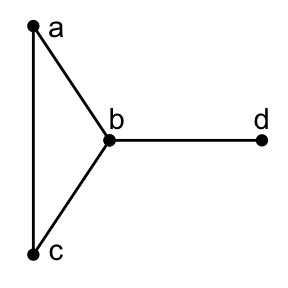
\includegraphics{t-algebra_files/figure-latex/four-vertex-group-1} \end{center}

\end{example}

Set \(n = |X|\), the order of \(\Gamma\).

Pick a field \(K\) (\(=\mathbb{R}\) or \(\mathbb{C}\)). Then \(\mathrm{Mat}_X(K)\) denotes the \(K\) algebra of all \(n\times n\) matrices with entries in \(K\). (rows and columns are indexed by \(X\))

\emph{Adjacency matrix} \(A\in \mathrm{Mat}_X(K)\) is defined by
\begin{align}
A_{xy} & = \left\{\begin{array}{cl} 1 & \textrm{ if } \; xy\in E,\\
0 & \textrm{ else.} \end{array}\right.
\end{align}

\begin{example}
\protect\hypertarget{exm:adjacency-matrix}{}\label{exm:adjacency-matrix}Let \(a, b, c, d\) be labels of rows and columns. Then
\[A = \begin{matrix} \\ a\\ b\\c\\d\end{matrix}\begin{matrix}\begin{matrix} a & b & c & d \end{matrix}\\\begin{pmatrix} 0 & 1 & 1 & 0 \\ 1 & 0 & 1 & 1 \\
1 & 1 & 0 & 0 \\ 0 & 1 & 0 & 0 \end{pmatrix}\end{matrix}\]
\end{example}

The subalgebra \(M\) of \(\mathrm{Mat}_X(K)\) generated by \(A\) is called the \emph{Bose-Mesner algebra} of \(\Gamma\).

Set \(V = K^n\), the set of \(n\)-dimensional column vectors, the coordinates are indexed by \(X\).

Let \(\langle\; , \;\rangle\) denote the Hermitean inner product:
\[\langle u, v\rangle = u^\top\cdot \bar{v} \quad (u, v\in V)\]
\(V\) with \(\langle\; , \;\rangle\) is the \emph{standard module} of \(\Gamma\).

\(M\) acts on \(V\): For every \(x\in X\), write
\[\hat{x} = \begin{pmatrix} 0 \\ \vdots \\ 0 \\ 1 \\ 0 \\ \vdots \\ 0 \end{pmatrix}\begin{matrix}  \\  \\  \leftarrow x \\  \\  \\ \end{matrix}\]
where \(1\) is at the \(x\) position.

Then
\[A\hat{x} = \sum_{y\in X, xy\in E}\hat{y}.\]
Since \(A\) is a real symmetrix matrix,
\[V = V_0 + V_1 + \cdots + V_r \quad \textrm{ some } r\in \mathbb{Z}^{\geq0},\]
the orthogonal direct sum of maximal \(A\)-eigenspaces.

Let \(E_i\in\mathrm{Mat}_X(K)\) denote the orthogonal projection,
\[E_i: V \longrightarrow V_i.\]
Then \(E_0, \ldots, E_r\) are the primitive idempotents of \(M\).
\[M = \mathrm{Span}_K(E_0, \ldots, E_r),\]
\[E_iE_j = \delta_{ij}E_i \quad \textrm{for all }\; i, j, \quad E_0 + \cdots + E_r = I.\]
Let \(\theta_i\) denote the eigenvalue of \(A\) for \(V_i\) in \(\mathbb{R}\). Without loss of generality we may assume that
\[\theta_0 > \theta_1 > \cdots > \theta_r.\]
Let
\[m_i = \textrm{the multiplicity of }\: \theta_i = \mathrm{dim} V_i = \mathrm{rank} E_i.\]
Set
\[\mathrm{Spec}(\Gamma) = \begin{pmatrix} \theta_0, & \theta_1, & \ldots, & \theta_r\\m_0, & m_1, & \ldots, & m_r\end{pmatrix}.\]
\textbf{Problem. }
What can we say about \(\Gamma\) when \(\mathrm{Spec}(\Gamma)\) is given?

The following Lemma \ref{lem:largestev}, is an example of Problem.

For every \(x\in X\),
\[k(x) \equiv \textrm{ valency of }x \equiv \textrm{ degree of }x \equiv |\{y\mid y\in X, \: xy\in E\}|.\]

\begin{definition}
\protect\hypertarget{def:regular}{}\label{def:regular}The graph \(\Gamma\) is \emph{regular}\index{regular} of valency\index{valency} \(k\) if \(k = k(x)\) for every \(x\in X\).
\end{definition}

\begin{lemma}
\protect\hypertarget{lem:largestev}{}\label{lem:largestev}

With the above notation,

\((i)\) \(\theta_0\leq \max\{k(x) \mid x\in X\} = k^{\max}\).\\
\((ii)\) If \(\Gamma\) is regular of valency \(k\), then \(\theta_0 = k\).

\end{lemma}

\hfill\break

\begin{proof}

\((i)\) Without loss of generality we may assume that \(\theta_0>0\), else done. Let \(v:=\sum_{x\in X}\alpha_x\hat{x}\) denote the eivenvector for \(\theta_0\).

Pick \(x\in X\) with \(|\alpha_x|\) maximal. Then \(|\alpha_x|\neq 0\).

Since \(Av = \theta_0v\),
\[\theta_0\alpha_x = \sum_{y\in X, xy\in E}\alpha_y.\]
So,
\[\theta_0 |\alpha_x| = |\theta_0\alpha_x| \leq \sum_{y\in X, xy\in E}|\alpha_y| \leq k(x)|\alpha_x| \leq k^{\max}|\alpha_x|.\]

\((ii)\) All 1's vector \(v = \sum_{x\in X}\hat{x}\) satisfies \(Av = kv\).

\end{proof}

\hfill\break

Let \(x, y\in X\) and \(\ell \in \mathbb{Z}^{\geq 0}\).

\begin{definition}
\protect\hypertarget{def:path}{}\label{def:path}A \emph{path}\index{path} of length \(\ell\) connecting \(x, y\) is a sequence
\[x = x_0, x_1, \ldots, x_{\ell} = y, \quad x_i\in X \quad (0\leq i\leq \ell)\]
such that \(x_ix_{i+1}\in E\) for all \(i\) \((0\leq i \leq \ell-1)\).
\end{definition}

\begin{definition}
\protect\hypertarget{def:distance}{}\label{def:distance}The \emph{distance}\index{distance} \(\partial(x,y)\) is the length of a shortest path connecting \(x\) and \(y\).
\[\partial(x,y) \in \mathbb{Z}^{\geq 0} \cup \{\infty\}.\]
\end{definition}

\begin{definition}
\protect\hypertarget{def:connected}{}\label{def:connected}The graph \(\Gamma\) is \emph{connected}\index{connected} if and only if \(\partial(x,y) < \infty\) for all \(x, y\in X\).

From now on, assume that \(\Gamma\) is connected with \(|X|\geq 2\).

Set \index{diameter of $\Gamma$}
\[d_\Gamma = d = \max\{\partial(x,y)\mid x, y\in X\} \equiv \textit{the diameter of }\;\Gamma.\]
\end{definition}

\begin{definition}
\protect\hypertarget{def:diameter}{}\label{def:diameter}For each vertex \(x\in X\), \index{diameter wrt $x$}
\[d(x) = \textit{the diameter with respect to }\: x = \max\{\partial(x,y)\mid y\in X\} \leq d.\]
\end{definition}

Fix a `base' vertex \(x\in X\).

Observe that
\[V = V_0^* + V_1^* + \cdots + V_{d(x)}^* \quad \textrm{(orthogonal direct sum)},\]
where
\[V_i^* = \mathrm{Span}_K(\hat{y}\mid \partial(x,y) = i) \equiv V_i^*(x)\]
and \(V_i^* = V_i^*(x)\) is called the \(i\)-th subconstituent with respect to \(x\).

Let \(E_i^* = E_i^*(x)\) denote the orthogonal projection
\[E_i^*: V \longrightarrow V_i^*(x).\]
View \(E_i^*(x) \in \mathrm{Mat}_X(K)\). So, \(E_i^*(x)\) is diagonal with \(yy\) entry:
\[(E_i^*(x))_{yy} = \begin{cases} 1 & \textrm{if } \: \partial(x,y) = i,\\ 0 & \textrm{else,}\end{cases} \quad \textrm{ for } y\in X.\]
Set
\[M^* = M^*(x) \equiv \textrm{Span}_K(E_0^*(x), \ldots, E_{d(x)}^*(x)).\]
Then \(M^*(x)\) is a commutative subalgebra of \(\mathrm{Mat}_X(K)\) and is called the \emph{dual Bose-Mesner algbara with respect to \(x\)}.

\begin{definition}[Subconstituent Algebra]
\protect\hypertarget{def:t-algebra}{}\label{def:t-algebra}Let \(\Gamma = (X, E)\), \(x\), \(M\), \(M^*(x)\) be as above. Let \(T = T(x)\) denote the subalgebra of \(\mathrm{Mat}_X(K)\) generated by \(M\) and \(M^*(x)\). \(T\) is the \emph{subconstituent algebra}\index{subconstituent algebra} of \(\Gamma\) with respect to \(x\).
\end{definition}

\begin{definition}
\protect\hypertarget{def:module}{}\label{def:module}A \(T\)-module \index{module} is any subspace \(W\subseteq V\) such that \(aw\in W\) for all \(a\in T\) and \(w\in W\).

\(T\)-module \(W\) is \emph{irreducible} \index{irreducible} if and only if \(W\neq 0\) and \(W\) does not properly contain a nonzero \(T\)-module.
\end{definition}

For any \(a\in \mathrm{Mat}_X(K)\), let \(a^*\) denbote the conjugate transpose of \(a\).

Observe that
\[\langle au, v\rangle = \langle u, a^*v\rangle \quad \textrm{for all }\; a\in \mathrm{Mat}_X(K), \textrm{ and for all } \; u,v\in V.\]

\begin{lemma}
\protect\hypertarget{lem:complete-reducibility}{}\label{lem:complete-reducibility}

Let \(\Gamma = (X,E)\), \(x\in X\) and \(T \equiv T(x)\) be as above.

\((i)\) If \(a\in T\), then \(a^*\in T\).

\((ii)\) For any \(T\)-module \(W\subset V\),

\[W^\bot := \{v\in V\mid \langle w, v\rangle = 0, \textrm{ for all }w\in W\}\]
is a \(T\)-module.

\((iii)\) \(V\) decomposes as an orthogonal direct sum of irreducible \(T\)-modules.

\end{lemma}

\hfill\break

\begin{proof}
\((i)\) It is becase \(T\) is generated by symmetric real matrices
\[A, E^*_0(x), E^*_1(x), \ldots, E^*_{d(x)}(x).\]

\((ii)\) Pick \(v\in W^\bot\) and \(a\in T\), it suffices to show that \(av\in W^\bot\). For all \(w\in W\),

\[\langle w, av\rangle = \langle a^*w, v\rangle = 0\]
as \(a^*\in T\).

\((iii)\) This is proved by the induction on the dimension of \(T\)-modules. If \(W\) is an irreducible \(T\)-module of \(V\), then

\[V = W + W^\bot \quad \textrm{(orthogonal direct sum)}.\]
\end{proof}

\textbf{Problem. }
What does the structure of the \(T(x)\)-module tell us about \(\Gamma\)?

Study those \(\Gamma\) whose modules take `simple' form. The \(\Gamma\)'s involved are highly regular.

\leavevmode\vadjust pre{\hypertarget{first-memo}{}}%
\textbf{HS MEMO}

\begin{enumerate}
\def\labelenumi{\arabic{enumi}.}
\tightlist
\item
  The subconstituent algebra \(T\) is semisimple as the left regular representation of \(T\) is completely reducible. See Curtis-Reiner 25.2 \citep{cr}.
\item
  The inner product \(\langle a, b\rangle_T = \mathrm{tr}(a^\top\bar{b})\) is nondegenerate on \(T\).
\item
  In general,
  \begin{align*}
  T\textrm{: Semisimple and Artinian} & \Leftrightarrow T\textrm{: Artinian with } J(T) = 0 \\
  & \Leftarrow T\textrm{: Artinian with nonzero nilpotent element} \\
  & \Leftarrow T \subset \mathrm{Mat}_X(K) \textrm{ such that for all } a\in T \textrm{ is normal.}
  \end{align*}
\end{enumerate}

\hypertarget{lec2}{%
\chapter{Perron-Frobenius Theorem}\label{lec2}}

\textbf{Friday, January 22, 1993}

In this lecture, we use the Perron Frobenius theory of non-negative matrices to obtain information on eigenvalues of a graph.

Let \(K = \mathbb{R}\). For \(n\in \mathbb{Z}^{> 0}\), pick a symmetric matrix \(C\in \mathrm{Mat}_n(\mathbb{R})\).

\begin{definition}
\protect\hypertarget{def:reducible}{}\label{def:reducible}The matrix \(C\) is \emph{reducible}\index{reducible} if and only if there is a bipartition \(\{1, 2, \ldots, n\} = X^+ \cup X^-\) (disjoint union of nonempty sets) such that \(C_{ij} = 0\) for all \(i\in X^+\), and for all \(j\in X^-\), and for all \(i\in X^-\), and for all \(j\in X^+\), i.e.,
\[ C \sim \begin{pmatrix} \ast & O \\ O & \ast \end{pmatrix}.\]
\end{definition}

\begin{definition}
\protect\hypertarget{def:bipartite-mat}{}\label{def:bipartite-mat}The matrix \(C\) is \emph{bipartite}\index{bipartite} if and only if there is a bipartition \(\{1, 2, \ldots, n\} = X^+ \cup X^-\) (disjoint union of nonempty sets) such that \(C_{ij} = 0\) for all \(i,j\in X^+\), and for all \(i,j\in X^-\), i.e.,
\[ C \sim \begin{pmatrix} O & \ast \\ \ast  & O \end{pmatrix}.\]
\end{definition}

\textbf{Note.}

\begin{enumerate}
\def\labelenumi{\arabic{enumi}.}
\tightlist
\item
  If \(C\) is bipartite, for every eigenvalue \(\theta\) of \(C\), \(-\theta\) is an eigenvalue of \(C\) such that \(\mathrm{mult}(\theta) = \mathrm{mult}(-\theta)\).
\end{enumerate}

Indeed, let \(C = \begin{pmatrix} O & A \\ B & O \end{pmatrix}\),
\[\begin{pmatrix} O & A \\ B & O \end{pmatrix} \begin{pmatrix}x\\y\end{pmatrix} = \theta \begin{pmatrix}x\\y\end{pmatrix}\Leftrightarrow \begin{pmatrix} O & A \\ B & O \end{pmatrix} \begin{pmatrix}x\\-y\end{pmatrix} = -\theta \begin{pmatrix}x\\-y\end{pmatrix}, \]
where \(Ay = \theta x\) and \(Bx = \theta y\).

\begin{enumerate}
\def\labelenumi{\arabic{enumi}.}
\setcounter{enumi}{1}
\item
  If \(C\) is bipartite, \(C^2\) is reducible.
\item
  The matrix \(C\) is irreducible and \(C^2\) is reducible, if \(C_{ij} \geq 0\) for all \(i,j\) and \(C\) is bipartite. (Exercise)
\end{enumerate}

\textbf{HS MEMO}

Note 1. Even if \(C\) is not symmetric
\[\begin{pmatrix} O & A \\ B & O \end{pmatrix} \begin{pmatrix}x\\y\end{pmatrix} = \theta \begin{pmatrix}x\\y\end{pmatrix}\Leftrightarrow \begin{pmatrix} O & A \\ B & O \end{pmatrix} \begin{pmatrix}x\\-y\end{pmatrix} = -\theta \begin{pmatrix}x\\-y\end{pmatrix}\]
holds. So the geometric multiplicities of \(\theta\) and \(-\theta\) coincide. How about the algebraic multiplicities?

Note 3. Set \(x \sim y\) if and only if \(C_{xy}>0\). So the graph may have loops. Then
\[(C^2)_{xy} > 0 \Leftrightarrow \textrm{ if there exists } z\in X \textrm{ such that } x\sim z \sim y.\]
Note that \(C\) is irreducible if and only if \(\Gamma(C)\) is connected. Let
\begin{align}
X^+ & = \{y\mid \textrm{there is a path of even length from }x \textrm{ to }y\}\\
X^- & = \{y\mid \textrm{there is no path of even length from }x \textrm{ to }y\} \neq \emptyset.
\end{align}
If there is an edge \(y\sim z\) in \(X^+\) and \(w\in X^-\). Then there would be a path from \(x\) to \(y\) of even length.
So \(\mathrm{e}(X^+, X^+) = \mathrm{e}(X^-, X^-) = 0.\).

\hfill\break

\begin{theorem}[Perron-Frobenius]
\protect\hypertarget{thm:pf}{}\label{thm:pf}

Given a matrix \(C\) in \(\mathrm{Mat}_n(\mathbb{R})\) such that

\((a)\) \(C\) is symmetric.

\((b)\) \(C\) is irreducible.

\((c)\) \(C_{ij} \geq 0\) for all \(i,j\).

Let \(\theta_0\) be the maximal eigenvalue of \(C\) with eigenspace \(V_0 \subseteq \mathbb{R}^n\), and let \(\theta_r\) be the minimal eigenvalue of \(C\) with eigenspace \(V_r \subseteq \mathbb{R}^n\). Then the following hold.

\((i)\) Suppose \(0\neq v = \begin{pmatrix}\alpha_1\\\alpha_2\\\vdots\\\alpha_n\end{pmatrix} \in V_0\). Then \(\alpha_i > 0\) for all \(i\), or \(\alpha_i < 0\) for all \(i\).

\((ii)\) \(\mathrm{dim}V_0 = 1\).

\((iii)\) \(\theta_r \geq -\theta_0\).

\((iv)\) \(\theta_r = \theta_0\) if and only if \(C\) is bipartite.

\end{theorem}

\hfill\break

First, we prove the following lemma.

\begin{lemma}
\protect\hypertarget{lem:pfl}{}\label{lem:pfl}Let \(\langle \;,\; \rangle\) be the dot product in \(V = \mathbb{R}^n\). Pick a symmetric matrix \(B \in \mathrm{Mat}_n(\mathbb{R})\). Suppose all eigenvalues of \(B\) are nonnegative. (i.e., \(B\) is positive semidefinite.) Then there exist vectors \(v_1, v_2, \ldots, v_n\in V\) such that \(B_{ij} = \langle v_i, v_j\rangle\) for all \(i,j\) \((1\leq i, j \leq n)\).
\end{lemma}

\begin{proof}
By elementary linear algebra, there exists an orthonormal basis \(w_1, w_2, \ldots, w_n\) of \(V\) consisting of eigenvectors of \(B\). Set the \(i\)-th column of \(P\) is \(w_i\) and \(D = \mathrm{diag}(\theta_1,\ldots, \theta_n)\). Then \(P^\top P = I\) and \(BP = PD\).

Hence,
\[B = PDP^{-1} = PDP^\top = QQ^\top,\]
where
\[Q = P\cdot \mathrm{diag}(\sqrt{\theta_1}, \sqrt{\theta_2}, \ldots, \sqrt{\theta_n}) \in \mathrm{Mat}_n(\mathbb{R}).\]
Now, let \(v_i\) be the \(i\)-th column of \(Q^\top\). Then
\[B_{ij} = v_i^\top\cdot v_j = \langle v_i, v_j\rangle.\]
This proves the lemma.
\end{proof}

Now we start the proof of Theorem \ref{thm:pf}.

\begin{proof}
\((i)\) Let \(\langle \text{ }, \text{ }\rangle\) denote the dot product on \(V = \mathbb{R}^n\). Set
\begin{align}
B & = \theta I - C\\
  & = \textrm{symmetric matrix with eigenvalues }\theta_0 - \theta_i \geq 0\\
  & = (\langle v_i, v_j\rangle)_{1\leq i,j\leq n}
\end{align}
with the same \(v_1, \ldots, v_n \in V\) by Lemma \ref{lem:pfl}.

Observe:
\[\sum_{i = 1}^n \alpha_iv_i = 0.\]

\emph{Pf.}
\begin{align}
\left\|\sum_{i = 1}^n \alpha_iv_i\right\|^2 & = \left\langle \sum_{i=1}^n\alpha_iv_i, \sum_{i=1}^n\alpha_iv_i\right\rangle\\
& = \begin{pmatrix} \alpha_1 &\ldots &\alpha_n\end{pmatrix}B\begin{pmatrix} \alpha_1\\\vdots\\\alpha_n\end{pmatrix}\\
& = v^\top Bv\\
& = 0,
\end{align}
since \(Bv = (\theta_0 I - C)v = 0\).

Now set
\[s = \textrm{the number of indices} \; i, \textrm{ where } \alpha_i >0.\]
Replacing \(v\) by \(-v\) if necessary, without loss of generality we may assume that \(s\geq 1\). We want to show \(s = n\).

Assume \(s < n\). Without loss of generality, we may assume that \(\alpha_i >0\) for \(1\leq i\leq s\) and \(\alpha_i \leq 0\) for \(s+1 \leq i \leq n\).
Set
\[ \rho = \alpha_1v_1 + \cdots + \alpha_sv_s = -\alpha_{s+1}v_{s+1} - \cdots - \alpha_nv_n.\]
Then, for \(i = 1,\ldots, s\),
\begin{align}
\langle v_i, \rho \rangle & = \sum_{j = s+1}^n -\alpha_j\langle v_i, v_j\rangle \quad (\langle v_i, v_j\rangle = B_{ij}, B = \theta_0I - C)\\
  & = \sum_{j = s+1}^n (-\alpha_{ij})(-C_{ij})\\
  & \leq 0.
\end{align}
Hence
\[0\leq \langle \rho, \rho\rangle = \sum_{i=1}^s \alpha_i \langle v_i, \rho\rangle \leq 0,\]
as \(\alpha_i > 0\) and \(\langle v_i, \rho\rangle \leq 0\). Thus, we have
\(\langle \rho, \rho \rangle = 0\) and \(\rho = 0\).
For \(j = s+1, \ldots, n\),
\[0 = \langle \rho, v_j\rangle = \sum_{i=1}^s \alpha_i\langle v_i, v_j\rangle \leq 0,\]
as \(\langle v_i, v_j\rangle = -C_{ij}\).

Therefore,
\[0 = \langle v_i, v_j \rangle = -C_{ij} \textrm{ for } 1\leq i \leq s, \: s+1 \leq j \leq n.\]
Since \(C\) is symmetric,
\[C = \begin{pmatrix} \ast & O \\ O & \ast\end{pmatrix}\]
Thus \(C\) is reducible, which is not the case. Hence \(s = n\).

\hfill\break

\((ii)\)
Suppose \(\dim V_0 \geq 2\). Then,
\[\dim\left(V_0 \cap \begin{pmatrix}1\\0\\\vdots\\0\end{pmatrix}^\bot\right) \geq 1.\]
So, there is a vector
\[0\neq v = \begin{pmatrix}\alpha_1\\\vdots\\\alpha_n\end{pmatrix} \in V_0\]
with \(\alpha_1 = 0\). This contradicts \((i)\).

Now pick
\[0\neq w = \begin{pmatrix}\beta_1\\\vdots\\\beta_n\end{pmatrix} \in V_r.\]

\((iii)\)
Suppose \(\theta_r < -\theta_0\). Since the eigenvalues of \(C^2\) are the squares of those of \(C\), \(\theta_r^2\) is the maximal eigenvalue of \(C^2\).

Also we have \(C^2w = \theta_r^2w\).

Observe that \(C^2\) is irreducible. (As otherwise, \(C\) is bipartite by Note 3, and we must have \(\theta_r = -\theta_0\).)
Therefore, \(\beta_i > 0\) for all \(i\) or \(\beta_i < 0\) for all \(i\). We have
\[\langle v, w\rangle = \sum_{i=1}^n\alpha_i\beta_j \neq 0.\]
This is a contradiction, as \(V_0 \bot V_r\).

\((iv)\)
\(\Rightarrow\): Let \(\theta_r = -\theta_0\). Then \(\theta = \theta_1^2 = \theta_0^2\) is the maximal eigenvalue of \(C^2\), and \(v\) and \(w\) are linearly independent eigenvalues for \(\theta\) for \(C^2\). Hence, for \(C^2\), \(\mathrm{mult}(\theta) \geq 2\).

Thus by \((ii)\), \(C^2\) must be reducible. Therefore, \(C\) is bipartite by Note 3.

\(\Leftarrow\): This is Note 1.
\end{proof}

Let \(\Gamma = (X, E)\) be any graph.

\begin{definition}
\protect\hypertarget{def:bipartite}{}\label{def:bipartite}\(\Gamma\) is said to be \emph{bipartite}\index{bipartite graph} if the adjacency matrix \(A\) is bipartite. That is, \(X\) can be written as a disjoint union of \(X^+\) and \(X^-\) such that \(X^+, X^-\) contain no edges of \(\Gamma\).
\end{definition}

\begin{corollary}
\protect\hypertarget{cor:spec}{}\label{cor:spec}

For any (connected) graph \(\Gamma\) with
\[\mathrm{Spec}(\Gamma) = \begin{pmatrix}\theta_0 & \theta_1 &\cdots & \theta_r\\m_1 & m_1 & \cdots & m_r\end{pmatrix} \:\textrm{ with }\: \theta_0 > \theta_1 > \cdots > \theta_r.\]
Let \(V_i\) be the eigenspace of \(\theta_i\). Then the following holds.

\begin{enumerate}
\def\labelenumi{\arabic{enumi}.}
\item
  Supppose \(0\neq v = \begin{pmatrix} \alpha_1\\\vdots \\\alpha_n \end{pmatrix} \in V_0\in \mathbb{R}^n\). Then \(\alpha_i > 0\) for all \(i\), or \(\alpha_i < 0\) for all \(i\).
\item
  \(m_0 = 1\).
\item
  \(\theta_r \geq -\theta_0\) if and only if \(\Gamma\) is bipartite. In this case,
  \[-\theta_i = \theta_{r-i} \; \textrm{and} \; m_i = m_{r-i} \quad (0\leq i\leq r).\]
\end{enumerate}

\end{corollary}

\begin{proof}
This is a direct consequences of Theorem \ref{thm:pf} and Note 3.
\end{proof}

\hypertarget{lec3}{%
\chapter{Cayley Graphs}\label{lec3}}

\textbf{Monday, January 25, 1993}

Given graphs \(\Gamma = (X, E)\) and \(\Gamma' = (X', E')\).

\begin{definition}
\protect\hypertarget{def:isom}{}\label{def:isom}

A map \(\sigma: X \to X'\) is an \emph{isomorphism}\index{isomorophism} of graphs whenever;

\begin{enumerate}
\def\labelenumi{\roman{enumi}.}
\tightlist
\item
  \(\sigma\) is one-to-one and onto,
\item
  \(xy\in E\) if and only if \(\sigma x \sigma y \in E'\) for all \(x, y\in X\).
\end{enumerate}

\end{definition}

We do not distinguish between isomorphic graphs.

\begin{definition}
\protect\hypertarget{def:auto}{}\label{def:auto}Suppose \(\Gamma = \Gamma'\). Above isomorphism \(\sigma\) is called an \emph{automorphism}\index{automorphism} of \(\Gamma\). Then set \(\mathrm{Aut}(\Gamma)\) of all automorphisms of \(\Gamma\) becomes a finite group under composition.
\end{definition}

\begin{definition}
\protect\hypertarget{def:transitive}{}\label{def:transitive}If \(\mathrm{Aut}(\Gamma)\) acts transitive on \(X\), \(\Gamma\) is called \emph{vertex transitive}\index{vertex transitive}.
\end{definition}

\begin{definition}[Cayley Graphs]
\protect\hypertarget{def:cayley}{}\label{def:cayley}Let \(G\) be any finite group, and \(\Delta\) any generating set for \(G\) such that \(1_G \not\in \Delta\) and \(g\in \Delta \to g^{-1}\in \Delta\).
Then Cayley graph \(\Gamma = \Gamma(G, \Delta)\) is defined on the vetex set \(X = G\) with the edge set \(E\) define by the following. \index{Cayley graph}

\[E = \{(h_1,h_2)\mid h_1, h_2\in G, h_1^{-1}h_2\in \Delta\} = \{(h, hg) \mid h\in G, g\in \Delta\}.\]
\end{definition}

\begin{example}
\protect\hypertarget{exm:cyclic6}{}\label{exm:cyclic6}

\(G = \langle a \mid a^6 = 1\rangle\), \(\Delta = \{a, a^{-1}\}\).

\begin{center}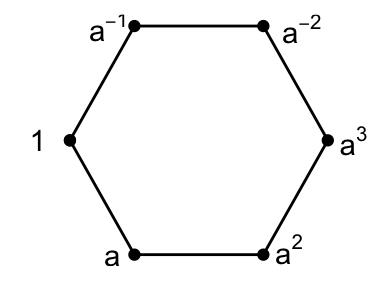
\includegraphics{t-algebra_files/figure-latex/unnamed-chunk-1-1} \end{center}

\end{example}

\begin{example}
\protect\hypertarget{exm:k6minus1}{}\label{exm:k6minus1}

\(G = \langle a \mid a^6 = 1\rangle\), \(\Delta = \{a, a^{-1}, a^2, a^{-2}\}\).

\begin{center}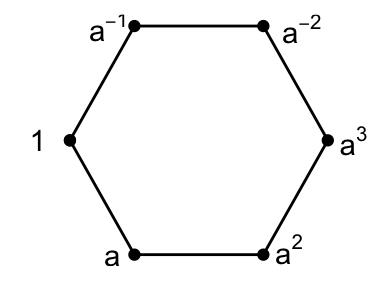
\includegraphics{t-algebra_files/figure-latex/unnamed-chunk-2-1} \end{center}

\end{example}

\begin{example}
\protect\hypertarget{exm:d6}{}\label{exm:d6}

\(G = \langle a, b \mid a^6 = 1 = b^2, ab = ba\rangle\), \(\Delta = \{a, a^{-1}, b\}\).

\begin{center}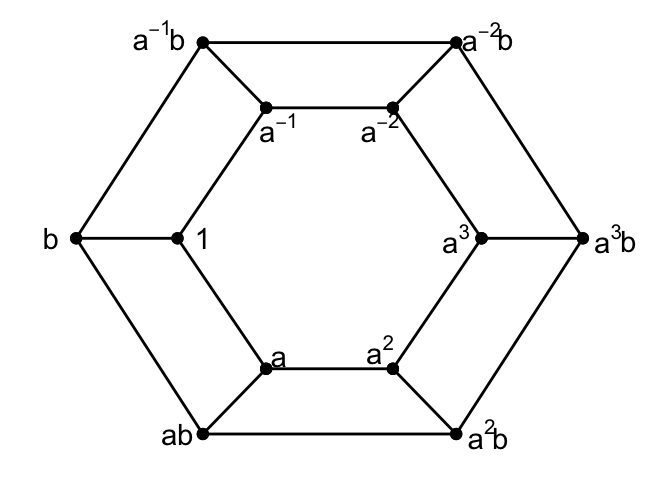
\includegraphics{t-algebra_files/figure-latex/unnamed-chunk-3-1} \end{center}

\end{example}

\textbf{HS MEMO}

\(\mathrm{Aut}(\Gamma) \simeq D_6\times \mathbb{Z}_2\) contains two regular subgroups isomorphic to \(D_6\) and \(\mathbb{Z}_6 \times \mathbb{Z}_2\) and \(\Gamma\) is obtained as Cayley graphs in two ways.

Cayley graphs are vertex transitive, indeed.

\begin{theorem}
\protect\hypertarget{thm:cayley-graph}{}\label{thm:cayley-graph}The following hold.

\((i)\) For any Cayley graph \(\Gamma = \Gamma(G, \Delta)\), the map

\[G \to \mathrm{Aut}(\Gamma) \; (g\mapsto \hat{g})\]
is an injective homomorphism of groups, where
\[\hat{g}(x) = gx \quad \textrm{for all }\: g\in G \textrm{ and for all } x\in X (= G).\]
Also, the image \(\hat{G}\) is regular on \(X\). i.e., the image \(\hat{G}\) acts transitively on \(X\) with trivial vertex stabilizers.

\((ii)\) For any graph \(\Gamma = (X, E)\), suppose there exists a subgroup \(G \subseteq \mathrm{Aut}(\Gamma)\) that is regular on \(X\). Pick \(x\in X\), and let

\[\Delta = \{g\in G\mid \langle x, g(x)\in E\}.\]
Then \(1\not\in \Delta\), \(g\in \Delta \to g^{-1}\in \Delta\), and \(\Delta\) generates \(G\). Moreover, \(\Gamma \simeq \Gamma(G, \Delta)\).
\end{theorem}

\begin{proof}
\((i)\) Let \(g\in G\). We want to show that \(\hat{g}\in \mathrm{Aut}(\Gamma)\). Let \(h_1, h_2\in X = G\). Then,
\begin{align}
(h_1, h_2)\in E & \to h_1^{-1}h_2\in \Delta\\
  & \to (gh_1)^{-1}(gh_2)\in \Delta \\
  & \to (gh_1, gh_2)\in E\\
  & \to (\hat{g}(h_1), \hat{g}(h_2)) \in E.
\end{align}
Hence, \(\hat{g}\in \mathrm{Aut}(\Gamma)\).

Observe: \(g \mapsto \hat{g}\) is a homomorphism of groups:
\[\hat{1}_G = 1, \; \widehat{g_1g_2} = \widehat{g_1}\widehat{g_2}.\]

Observe: \(g \mapsto \hat{g}\) is one-to-one:
\[\widehat{g_1} = \widehat{g_2} \to g_1 = \widehat{g_1}(1_G) = \widehat{g_2}(1_G) = g_2.\]

Observe: \(\hat{G}\) is regular on \(X\): Clear by construction.

\((ii)\) \(1_G\not\in \Delta\): Since \(\Gamma\) has not loops, \((x, 1_Gx) \not\in E\).

\(g\in \Delta \to g^{-1}\in \Delta\):
\[g\in \Delta \to (x, g(x))\in E \to E \ni (g^{-1}(x), g^{-1}(g(x))) = (g^{-1}(x), x).\]

\(\Delta\) generates \(G\): Suppose \(\langle \Delta \rangle \subsetneq G\). Let \(\hat{X} = \{g(x)\mid g\in \langle \Delta\rangle\} \subsetneq X\). (\(\hat{X} \subsetneq X\) as \(G\) acts regularly on \(X\).)

Since \(\Gamma\) is connected, there exists \(y\in \hat{X}\) and \(z\in X\setminus \hat{X}\) with \(yz\in E\).

Let \(y = g(x)\), \(g\in \langle \Delta\rangle\), \(z\in h(x)\), \(h\in G\setminus \langle \Delta\rangle\). Then
\[(y,z)=(g(x),h(x))\in E \to (x,g^{-1}h(x))\in E \to g^{-1}h\in \langle \Delta \rangle \to h\in \langle \Delta \rangle. \]
This is a contradition. Therefore, \(\Delta\) generates \(G\).

Let \(\Gamma' = (X', E')\) denote \(\Gamma(G, \Delta)\). We shall show that
\[\theta: X' \to X \; (g\mapsto g(x))\]
is an isomorphism of graphs.

\(\theta\) is one-to-one: For \(h_1, h_2\in X' = G\),
\[\theta(h_1)=\theta(h_2) \to h_1(x) = h_2(x) \to h_2^{-1}h_1(x)=x \to h_2^{-1}h_1\in \mathrm{Stab}_G(x) = \{1_G\} \to h_1 = h_2.\]
(\(\mathrm{Stab}_G(x) = \{g\in G\mid g(x) = x\}\).)

\(\theta\) is onto: Since \(G\) is transitive,
\[X = \{g(x)\mid g\in G\} = \theta(X') = \theta(G).\]

\(\theta\) respects adjacency: For \(h_1, h_2\in X' = G\),
\[(h_1,h_2)\in E' \leftrightarrow h_1^{-1}h_2\in \Delta \leftrightarrow (x, h_1^{-1}h_2(x))\in E \leftrightarrow (h_1(x),h_2(x))\in E \leftrightarrow (\theta(h_1), \theta(h_2))\in E.\]
Therefore \(\theta\) is an isomorphism between graphs \(\Gamma(G, \Delta)\) and \(\Gamma(X, E)\).
\end{proof}

How to compute the eigenvalues of the Cayley graph of and abelian group.

Let \(G\) be any finite abelian group. Let \(\mathbb{C}^*\) be the multiplicative group on \(\mathbb{C}\setminus \{0\}\).

\begin{definition}
\protect\hypertarget{def:character}{}\label{def:character}A (linear) \(G\)-character\index{character} is any group homomorphism \(\theta: G \to \mathbb{C}^*\).
\end{definition}

\begin{example}
\protect\hypertarget{exm:cyclic3}{}\label{exm:cyclic3}\(G = \langle a\mid a^3 =1\rangle\) has three characters, \(\theta_0, \theta_1, \theta_2\).
\[
\begin{array}{c|ccc}
\theta_i(a^j) & 1 & a & a^2 \\
\hline
\theta_0 & 1 & 1 & 1\\
\theta_1 & 1 & \omega & \omega^2\\
\theta_2 & 1 & \omega^2 & \omega
\end{array}, \quad \textrm{with }\; \omega = \frac{-1+\sqrt{-3}}{2}.
\]
Here \(\omega\) is a primitive cube root of \(q\) in \(\mathbb{C}^*\), i.e., \(1+\omega + \omega^2 = 0\).
\end{example}

For arbitraty group \(G\), let \(X(G)\) be the set of all characters of \(G\).

Observe: For \(\theta_1, \theta_2\in X(G)\), one can define product \(\theta_1\theta_2\):
\[\theta_1\theta_2(g) = \theta_1(g)\theta_2(g) \quad \textrm{for all }\; g\in G.\]
Then \(\theta_1\theta_2\in X(G)\).

Observe: \(X(G)\) with this product is an (abelian) group.

\begin{lemma}
\protect\hypertarget{lem:charactergroup}{}\label{lem:charactergroup}The groups \(G\) and \(X(G)\) are isomorphic for all finite abelian groups \(G\).
\end{lemma}

\begin{proof}
\(G\) is a direct sum of cyclic groups;
\[G = G_1\oplus G_2 \oplus \cdots \oplus G_m, \quad \textrm{where } \; G_i = \langle a_i\mid a_i^{d_i} = 1\rangle \quad (1\leq i\leq m).\]
Pick any element \(\omega_i\) of order \(d_i\) in \(\mathbb{C}^*\), i.e., a primitive \(d_i\)-the root of \(1\). Define
\[\theta_i: G \to \mathbb{C}^* \quad (a_1^{\varepsilon_1}\cdots a_m^{\varepsilon_m} \mapsto \omega_i^{\varepsilon_i} \quad \textrm{where }\; 0\leq \varepsilon_i < d_i, 1\leq i\leq m).\]
Then \(\theta_i\in X(G)\). (Exercise)

Claim: There exists an isomorphism of groups \(G \to X(G)\) that sends \(a_i\) to \(\theta_i\).

Observe: \(\theta_i^{d_i} = 1\). For every \(g = a_1^{\varepsilon_1}\cdots a_m^{\varepsilon_m} \in G\),
\[\theta_i^{d_i}(g) = (\theta_i(g))^{d_i} = (\omega_i^{\varepsilon_i})^{d_i} = (\omega_i^{d_i})^{\varepsilon_i} = 1.\]
Observe: If \(\theta_1^{\varepsilon_1}\theta_2^{\varepsilon_2}\cdots \theta_m^{\varepsilon_m} = 1\) for some \(0\leq \varepsilon_i < d_i, 1\leq i\leq m\). Then \(\varepsilon_1 = \varepsilon_2 = \cdots = \varepsilon_m = 0\).

\emph{Pf.} \(1 = \theta_1^{\varepsilon_1}\theta_2^{\varepsilon_2}\cdots \theta_m^{\varepsilon_m}(a_i) = \omega_i^{\varepsilon_i}\), Since \(\omega_i\) is a primitive \(d_i\)-th root of \(1\), \(\varepsilon_i = 0\) for \(1\leq i\leq m\).

Observe: \(\theta_1, \ldots, \theta_m\) generate \(X(G)\). Pick \(\theta\in X(G)\). Since
\(a_i^{d_i} = 1\), \(1 = \theta(a_i^{d_i}) = \theta(a_i)^{d_i}\).

Hence \(\theta(a_i) = \omega^{\varepsilon_i}\) for some \(\varepsilon_i\) with \(0\leq \varepsilon_i < d_i\).

Now \(\theta = \theta_1^{\varepsilon_1}\cdots \theta_m^{\varepsilon_m}\), since these are both equal to \(\omega_i^{\varepsilon_i}\) at \(a_i\) for \(1\leq i \leq m\).

Therefore,
\[G \to X(G) \quad (a_i \mapsto \theta_i)\]
is an isomorphism of groups.
\end{proof}

\textbf{Note.} The correspondence above is clearly a group homomorphism.

\hypertarget{lec4}{%
\chapter{Examples}\label{lec4}}

\textbf{Wednesday, January 27, 1993}

\begin{theorem}
\protect\hypertarget{thm:charcter-group}{}\label{thm:charcter-group}Given a Cayley graph \(\Gamma = \Gamma(G, \Delta)\). View the standard module \(V \equiv \mathbb{C}G\) (the group algebra), so
\[\left\langle \sum_{g\in G}\alpha_g g, \;\sum_{g\in G}\beta_g g\right\rangle = \sum_{g\in G}\alpha_g\overline{\beta_g}, \quad \textrm{with}\; \alpha_g, \beta_g\in \mathbb{C}.\]
For any \(\theta\in X(G)\), write
\[\hat{\theta} = \sum_{g\in G}\theta(g^{-1})g.\]
Then the following hold.

~~\((i)\) \(\langle \hat{\theta_1}, \hat{\theta_2}\rangle = |G|\) if \(\theta_1 = \theta_2\) and \(0\) othewise for \(\theta_1, \theta_2\in X(G)\). In particular, \(\{\hat{\theta}\mid \theta\in X(G)\}\) forms a basis for \(V\).

~~\((ii)\) \(A\hat{\theta} = \Delta_\theta \hat{\theta}\) for \(\theta \in X(G)\), where \(A\) is the adjacency matrix and

\[\Delta_\theta = \sum_{g\in \Delta}\theta(g).\]
In particular, the eigenvalues of \(\Gamma\) are precisely
\[\{\Delta_\theta \mid \theta\in X(G)\}.\]
\end{theorem}

\begin{proof}
\leavevmode

\((i)\) Claim: For every \(\theta \in X(G)\), let

\[s:= \sum_{g\in G}\theta(g^{-1}) = \begin{cases} |G| & \text{if }\;\theta = 1\\
0 & \text{if } \;\theta \neq 1. 
\end{cases}\]
\emph{Pf.} Clear if \(\theta =1\).

Let \(\theta \neq 1\). Then \(\theta(h)\neq 1\) for some \(h\in G\).
\[s\cdot \theta(h) = \left(\sum_{g\in G}\theta(g^{-1})\right)\theta(h) = \sum_{g\in G}\theta(g^{-1}h) = \sum_{g'\in G}\theta(g'^{-1}) = s.\]
Since \(\theta(h)\neq 1\), \(s = 0\).

Claim. \(\theta(g^{-1}) = \overline{\theta(g)}\) for every \(\theta\in X(G)\) and every \(g\in G\).

Since \(\theta(g)\in \mathbb{C}\) is a root of \(1\),
\[|\theta(g)|^2 = \theta(g)\overline{\theta(g)} = 1.\]
On the other hand, since \(\theta\) is a homomorphism,
\[\theta(g)\theta(g^{-1}) = \theta(1) = 1.\]
Hence \(\theta(g^{1}) = \overline{\theta(g)}\).

Now
\begin{align}
\langle \widehat{\theta_1}, \widehat{\theta_2}\rangle & = \sum_{g\in G}\theta_1(g^{-1})\overline{\theta_2(g^{-1})}\\
& = \sum_{g\in G}\theta_1(g^{-1})\theta_2(g)\\
& = \sum_{g\in G}\theta_1\theta_2^{-1}(g^{-1})\\
& = \begin{cases} |G| & \text{if}\quad \theta_1\theta_2^{-1} = 1\\
0 & \text{if} \quad \theta_1\theta_2^{-1}\neq 1.
\end{cases}
\end{align}
Since \(|G| = |X(G)|\) by Lemma \ref{lem:charactergroup}, and \(\widehat{\theta_i}\)'s are orthogonal nonzero elements in \(V\), that form a basis of \(V\).

~\((ii)\) Let \(\Delta = \{g_1, \ldots, g_r\}\). Then

\begin{align}
A\hat{\theta} & = A\left(\sum_{g\in G}\theta(g^{-1}g)\right)\\
& = \sum_{g\in G}\theta(g^{-1})(gg_1 + \cdots + gg_r) \quad (\Gamma(g) = \{gg_1, \ldots, gg_r\})\\
& = \sum_{i = 1}^r \left(\sum_{g\in G}\theta(g^{-1})(gg_i)\right)\\
& = \sum_{i=1}^r\left(\sum_{g\in G}\theta(g_ig_i^{-1}g^{-1})(gg_i)\right)\\
& = \sum_{i = 1}^r\left(\sum_{g\in G}\theta(g_i)\theta((gg_i)^{-1})gg_i\right)\\
& = \sum_{i = 1}^r\theta(g_i)\sum_{h\in G}\theta(h^{-1})h \\
& = \Delta_\theta\cdot \hat{\theta}.
\end{align}
Since \(\{\hat{\theta}\mid \theta\in X(G)\}\) forms a basis, the eigenvalues of \(\Gamma\) are precisely,
\[\{\Delta_\theta\mid \theta\in X(G)\}.\]

This completes the proof.

\end{proof}

\begin{example}
\protect\hypertarget{exm:character-cyclic6}{}\label{exm:character-cyclic6}Let \(G = \langle a\mid a^6 = 1\rangle\), and \(\Delta = \{a, a^{-1}\}\). Pick a primitive 6-th root of 1, \(\omega\). Then
\[X(G) = \{\theta^i\mid 0\leq i\leq 5\} \quad \text{such that }\quad \theta(a) = \omega, \; \omega + \omega^{-1} = 1.\]

\begin{center}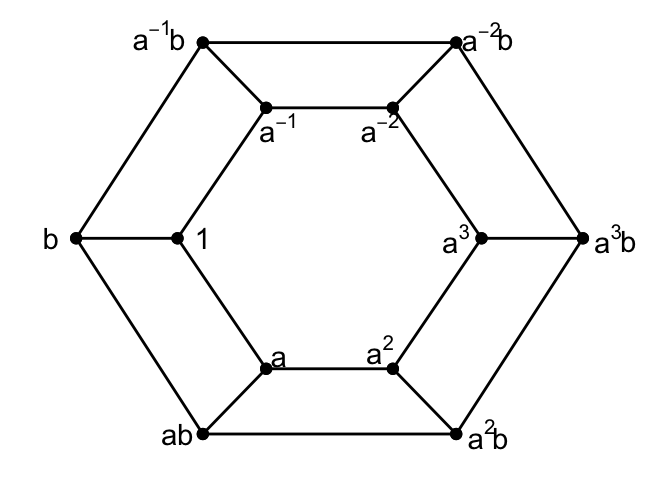
\includegraphics{t-algebra_files/figure-latex/unnamed-chunk-4-1} \end{center}

\[\begin{array}{c | c | c}
\varphi\in X(G) & \varphi(a) & \Delta_\varphi = \theta(a) + \theta(a)^{-1}\\
\hline
1 & 1 & 2\\
\theta & \omega & \omega+\omega^{-1} = 1\\
\theta^2 & \omega^2 & -1\\
\theta^3 & \omega^3 = -1 & -2\\
\theta^4 & \omega^4 & -1\\
\theta^5 & \omega^5 & 1
\end{array}\]
\[\text{Spec}(\Gamma) = \begin{pmatrix} 2 & 1 & -1 & -2\\ 1 & 2 & 2 & 1\end{pmatrix}.\]
\end{example}

\begin{example}
\protect\hypertarget{exm:hd2}{}\label{exm:hd2}\(D\)-cube, \(H(D,2)\). Let
\[X = \{(a_1, \ldots, a_D)\mid a_i\in \{1,-1\}, \; 1\leq i\leq D\},\]
\[E = \{xy\mid x, y\in X, \; x, y \text{: different in exactly one coordinate}\}.\]
Also \(H(D,2)\) is a Cayley graph \(\Gamma(G, \Delta)\), where
\[G = G_1\oplus G_2 \oplus \cdots \oplus G_D, \]
\[G_i = \langle a_i\mid a_i^2  = 1\rangle,\quad \Delta = \{a_1, \ldots, a_D\}.\]
\end{example}

\textbf{Homework}: The spectrum of \(H(D,2)\) is
\[\begin{pmatrix} \theta_0 & \theta_1 & \cdots & \theta_D\\
m_0 & m_1 & \cdots & m_D\end{pmatrix},\]
where
\[\theta_i = D-2i \quad (0\leq i\leq D), \quad m_i = \binom{D}{i}.\]

\textbf{HS MEMO}

Let \(\theta \in X(G)\). Then \(\theta: X \to \{\pm 1\}\). If
\[\nu(\theta) = |\{i\mid \theta(a_i) = -1\}|, \]
then \(\Delta_\theta = D-2i\). Since there are \(\binom{D}{i}\) such \(\theta\), we have te assertion.

We want to compute the subconstituent algebra for \(H(D,2)\). First, we make a few observations about arbitrary graphs.

Let \(\Gamma = (X,E)\) be any graph, \(A\), the adjacemcy matrix of \(\Gamma\), and \(V\), the standard module over \(K = \mathbb{C}\).

Fix a base \(x\in X\). Write \(E_i^* = E_i^*(x)\), and
\[T \equiv T(x) = \text{the algebra generated by}\; A, E_0^*, E_1^*, \ldots .\]

\begin{definition}
\protect\hypertarget{def:rd}{}\label{def:rd}Let \(W\) be any irreducible \(T\)-module (\(\subseteq V\)). Then the endpoint\index{endpoint} \(r \equiv r(W)\) satisfied
\[r = \min\{i\mid E_i^*W \neq 0\}.\]
The diameter\index{diameter} \(d = d(W)\) satisfied
\[d = |\{i\mid E_i^*W \neq 0\}| - 1.\]
\end{definition}

\begin{lemma}
\protect\hypertarget{lem:irreducible}{}\label{lem:irreducible}

With the above notation, let \(W\) be an irreducible \(T\)-module. Then

\((i)\) \(E_i^*AE_j^* = 0 \; \text{ if }\; |i-j|>1, \; E_i^*AE_j^*\neq 0 \; \text{ if }\; |i-j| = 1, \quad 0\leq i,j\leq d(x)\).\\
\((ii)\) \(AE_j^*W \subseteq E_{j-1}^*W + E_j^*W + E^*_{j+1}W\), \(0\leq j \leq d(x)\). \((E_i^*W = 0 \; \text{ if } i<j\) or \(i > d(x)\).)\\
\((iii)\) \(E^*_jW \neq 0\) if \(r\leq j \leq r+d\), \(=0\) if \(0\leq j\leq r\) or \(r+d < j \leq d(x)\).\\
\((iv)\) \(E_i^*AE^*_jW \neq 0\), if \(|i-j| = 1\) \((r \leq i,j \leq r+d)\).

\end{lemma}

\begin{proof}
\leavevmode

\((i)\) Pick \(y\in X\) with \(\partial(x,y) = j\). We want to find \(E_i^*AE^*_j \hat{y}\). Note,

\[E_j^*\hat{y} = \begin{cases} 0 & \text{if }\; \partial(x.y)\neq j\\
\hat{y} & \text{if }\; \partial(x,y) = j.\end{cases}.\]
\begin{align}
E_i^*AE_j^*\hat{y} &= E_i^*A\hat{y} \\
& = E_i^*\sum_{z\in X, yz\in E}\hat{z}\\
& = \sum_{z\in X, yz\in E, \partial(x, z) = i}\hat{z}  \label{eq:eiaeejy}\\
& = 0 \; \text{ if }\; |i-j|>1 && \text{by triangle inequality.}
\end{align}
If \(|i-j| = 1\), there exist \(y, y'\in X\) such that \(\partial(x,y) = j\), \(\partial(x,y') = i\), \(yy'\in E\) by connectivity of \(\Gamma\). Hence
\eqref{eq:eiaeejy} contains \(\widehat{y'}\) and \eqref{eq:eiaeejy} is not equal to zero.

\((ii)\) We have

\begin{align}
AE_j^*W & = \left(\sum_{i=0}^{d(x)}E_i^*\right)AE_j^*W\\
& = E_{j-1}^*AE^*_jW + E^*_jAE_j^*W + E^*_{j+1}AE_j^*W\\
& \subseteq E^*_{j-1}W + E^*_jW + E^*_{j+1}W.
\end{align}

\((iii)\) Suppose \(E_j^*W = 0\) for some \(j\) \((r\leq j \leq r+d)\). Then \(r < j\) by the definition of \(r\). Set

\[\widetilde{W} = E^*_rW + E^*_{r+1}W + \cdots + E^*_{j-1}W.\]
Observe \(0\subsetneq \widetilde{W} \subsetneq W\).
Also \(A\widetilde{W} \subseteq \widetilde{W}\) by \((ii)\), and \(E_i^*\widetilde{W} \subseteq \widetilde{W}\) for every \(i\) by construction.

Thus, \(T\widetilde{W} \subseteq \widetilde{W}\), contradicting \(W\) being irreducible.

\end{proof}

\hypertarget{lec5}{%
\chapter{\texorpdfstring{\(T\)-Modules of \(H(D,2)\), I}{T-Modules of H(D,2), I}}\label{lec5}}

\textbf{Friday, January 29, 1993}

Let \(\Gamma = (X, E)\) be a graph, \(A\) the adjacency matrix, and \(V\) the standard module over \(K = \mathbb{C}\).

Fix a base \(x\in X\) and write \(E_i^* \equiv E_i^*(x)\), and \(T \equiv T(x)\).

Let \(W\) be an irreducible \(T\)-module with endpoint \(r:= \min\{i\mid E_i^*W \neq 0\}\) and diameter \(d:=|\{i\mid E_i^*W\neq 0\}|-1\).

We have
\begin{align}
{E^*_i}W & \neq 0 & r\leq i \leq r+d\\
& = 0 & 0 \leq i < r \;\text{ or }\; r+d < i \leq d(x).
\end{align}

Claim: \(E_i^*AE_j^*W \neq 0\) if \(|i-j| = 1\) for \(r\leq i,j\leq r+d\). (See Lemma \ref{lem:irreducible}.)

Suppose \(E_{j+1}^*AE_j^*W = 0\) for some \(j\) with \(r \leq j < r+d\).
Observe that
\[\tilde{W} = E^*_rW + \cdots + E^*_jW\]
is \(T\)-invariant with
\[0 \subsetneq \tilde{W} \subsetneq W.\]
Becase \(A\tilde{W} \subseteq \tilde{W}\) since \(AE_j^*W \subseteq E^*_{j-1}W + E^*_jW\),
\[E_k^*\tilde{W} \subseteq \tilde{W} \quad\text{for all }\; k,\]
we have \(T\tilde{W} \subseteq{W}\).

Suppose \(E_{i-1}^*AE_i^*W = 0\) for some \(i\) with \(r \leq i < r+d\).

Similarly,
\[\tilde{W} = E^*_iW + \cdots + E^*_{r+d}W\]
is a \(T\)-module with \(0\subsetneq \tilde{W} \subsetneq W\).

\begin{definition}
\protect\hypertarget{def:isomorphic-modules}{}\label{def:isomorphic-modules}Let \(\Gamma\), \(E^*_i\), and \(T\) be as above. Irreducible \(T\)-modules \(W\) and \(W'\) are isomorphic\index{isomorphic} whenever there is an isomorphism \(\sigma: W \to W'\) of vector spaces such that \(a\sigma = \sigma a\) for all \(a\in T\).
\end{definition}

Recall that the standard module \(V\) is an orthogonal direct sum of irreducible \(T\)-modules
\[W_1 \oplus W_2 \oplus \cdots \oplus W_{\ell}, \; \text{for some }\ell.\]
Given \(W\) in this list, the multiplicity\index{multiplicity} of \(W\) in \(V\) is
\[|\{j \mid W_j \simeq W\}|.\]

\textbf{HS MEMO}

It is known that the multiplicity does not depend on the decomposition.

Now assume that \(\Gamma\) is the \(D\)-cube, \(H(D,2)\) with \(D\geq 1\). View
\begin{align}
X & = \{a_1\cdots a_D\mid a_i\in \{1, -1\}, 1\leq i\leq D\},\\
E & = \{xy\mid x, y\in X, \; x, y \;\text{ differ in exactly 1 coordinate}\}.
\end{align}
Find \(T\)-modules.

Claim: \(H(D,2)\) is bipartite with a partition \(X = X^+ \cup X^-\), where
\begin{align}
X^+ & = \{a_1\cdots a_D\in X\mid \prod a_i > 0\}\\
X^- & = \{a_1\cdots a_D \in X \mid \prod a_i < 0\}
\end{align}

Observe: for all \(y, z\in X\),
\[\partial(y,z) = i \Leftrightarrow y, z \; \text{ differ in exactly in }\; i\; \text{ coorinates with }\; 0\leq i\leq D.\]
Here, the diameter of \(H(D, 2) = D = d\) for all \(x\in X\).

\begin{theorem}
\protect\hypertarget{thm:hd2-modules}{}\label{thm:hd2-modules}Let \(\Gamma = H(D,2)\) be as above. Fix \(x\in X\), and write \(E_i^* = E^*_i(x)\), and \(T = T(x)\).

Let \(W\) be an irreducible \(T\)-module with endpoint \(r\), and diameter \(d\) with \(0\leq r \leq r+d\leq D\).

\((i)\) \(W\) has a basis \(w_0, w_1, \ldots, w_d\) with \(w_i\in E^*_{i+r}W\) for \(0\leq i\leq d\). With respect to which the matrix representing \(A\) is

\[
\begin{pmatrix}
0 & d & 0 & \cdots & 0 & 0 & 0\\
1 & 0 & d-1 & \cdots & 0 & 0 & 0\\
0 & 2 & 0 & \cdots & 0 & 0 & 0\\
0 & 0 & 3 & \cdots & 0 & 0 & 0\\
\cdots & \cdots & \cdots & \ddots & \ddots & \cdots & \cdots \\
0 & 0 & 0 & \ddots & 0 & 2 & 0\\
0 & 0 & 0 & \cdots & d-1 & 0 & 1\\
0 & 0 & 0 & \cdots & 0 & d & 0
\end{pmatrix}
\]

\((ii)\) \(d= D-2r\). In particular, \(0\leq r\leq D/2\).

\((iii)\) Let \(W'\) denote an irreducible \(T\)-module with endpoint \(r'\). Then \(W\) and \(W'\) are isormorphic as \(T\)-modules if and only if \(r = r'\).

\((iv)\) The multiplicity of the irreducible \(T\)-module with endpoint \(r\) is

\[\binom{D}{r} - \binom{D}{r-1} \quad \text{if } 1\leq r \leq R/2,\]
and \(1\) if \(r = 0\).
\end{theorem}

\begin{proof}
Recall that \(\Gamma\) is vertex transitive. It is a Cayley graph.

Hence without loss of generality, we may assume that
\(x = \overbrace{11\cdots 1}^{D}\).

Notation: Set \(\Omega = \{1, 2, \ldots, D\}\). For every subset \(S \subseteq \Omega\), let
\[\hat{S} = a_1\cdots a_d \in X \quad a_i = \begin{cases} -1 & \text{if }\; i\in S\\ 1 & \text{if } i\not\in S.\end{cases}\]
In particular, \(\hat{\emptyset} = x\) and
\[|S| = i \Leftrightarrow \partial(x, \hat{S}) = i \Leftrightarrow \hat{S}\in E^*_iV.\]
For all \(S, T\subseteq \Omega\), we say \(S\) covers \(T\) if and only if \(S\supseteq T\) and \(|S| = |T| +1\).

Observe that \(\hat{S}, \hat{T}\) are adjacent in \(\Gamma\) if and only if either \(T\) coverse \(S\) or \(S\) coverr \(T\).

Define the `raising matrix'
\[R = \sum_{i=0}^D E^*_{i+1}AE^*_i.\]

Observe that
\[RE_i^*V \subseteq E^*_{i+1} V \; \text{ for }\; 0\leq i \leq D, \; \text{ and }E^*_{D+1}V = 0.\]
Indeed for any \(S\subseteq \Omega\) with \(|S| = i\),
\begin{align}
R\hat{S} & = RE^*_i\hat{S} \\
& = E^*_{i+1}A\hat{S} \\
& = \sum_{T_1 \subseteq \Omega, S \text{ covers }T_1} E^*_{i+1}\widehat{T_1} + \sum_{T \subseteq \Omega, T \text{ covers }S} E^*_{i+1}\hat{T}\\
& = \sum_{T \subseteq \Omega, T \text{ covers }S} E^*_{i+1}\hat{T}.
\end{align}

Define the `lowering matrix'
\[L = \sum_{i=0}^D E^*_{i-1}AE^*_i.\]

Observe that
\[LE_i^*V \subseteq E^*_{i-1}V \; \text{ for }\; 0\leq i \leq D, \; \text{ and }E^*_{-1}V = 0.\]
Indeed for any \(S\subseteq \Omega\),
\[L\hat{S} = \sum_{T\subseteq \Omega, S \text{ covers }T} \hat{T}.\]

Observe that \(A = L + R\).

For convenience, set
\[A^* = \sum_{i=0}^D (D-2i)E_i^*.\]

Claim: The following hold.

\((a)\) \(LR - RL = A^*\).\\
\((b)\) \(A^*L - LA^* = 2L\).\\
\((c)\) \(A^*R - RA^* = -2R\).

In particular \(\mathrm{Span}(R,L, A^*)\) is a 'representation of Lie algebra \(\mathrm{sl}_2(\mathbb{C})\).

\textbf{HS MEMO}

\[\mathrm{sl}_2(\mathbb{C}) = \{X\mid \mathrm{Mat}(\mathbb{C} \mid \mathrm{tr}(X) = 0\}.\]
For \(X, Y\in \mathrm{sl}_2(\mathbb{C})\), define a binary operation \([X, Y] = XY - YX\).
\[A^*\sim \begin{pmatrix} 1 & 0 \\ 0 & -1\end{pmatrix}, \quad L\sim \begin{pmatrix} 0 & 1 \\ 0 & 0\end{pmatrix}, \quad R\sim \begin{pmatrix} 0 & 0 \\ 1 & 0\end{pmatrix}.\]
Then these satisfy the relations \((a)\) - \((c)\) above.

\emph{Proof of Claim.}
Apply both sides to \(\hat{S}\) \quad \((S\subseteq \Omega)\). Say \(|S| = i\).

\emph{Proof of \((a)\):}
\begin{align} 
(LR - RL)\hat{S} & = L\left(\sum_{\substack{T \subseteq \Omega, T \text{ covers }S\\(D-i \text{ of them})}}\hat{T}\right) - R \left(\sum_{\substack{U \subseteq \Omega, S \text{ covers }U\\(i \text{ of them})}}\hat{U}\right)\\
& = (D-i)\hat{S} + \sum_{V \subseteq \Omega, |V| = i, |S\cap V| = i-1}\hat{V}\\
& \qquad - \left(i\hat{S} + \sum_{V \subseteq \Omega, |V| = i, |S\cap V| = i-1}\hat{V}\right)\\
& = (D-2i)\hat{S}\\
& = A^*\hat{S}.
\end{align}

\emph{Proof of \((b)\):}
\begin{align} 
(A^*L - LA^*)\hat{S} & = (D-2(i-1))L\hat{S} - (D-2i)L\hat{S} \quad (\text{since} \; L\hat{S}\in E^*_{i-1}V)\\
& = 2L\hat{S}.
\end{align}

\emph{Proof of \((c)\):}
\begin{align} 
(A^*R - RA^*)\hat{S} & = (D-2(i+1))R\hat{S} - (D-2i)R\hat{S} \quad (\text{since} \; R\hat{S}\in E^*_{i+1}V)\\
& = -2R\hat{S}.
\end{align}

Let \(W\) be an irreducible \(T\)-module with endpoint \(r\) and diameter \(d\) \((0\leq r \leq r+d \leq D)\).

\emph{Proof of \((i)\) and \((ii)\):}

Pick \(0\neq w \in E^*_rW\).

Claim: \(LRw = (D-2r)w\).

\emph{Pf.}
\begin{align} 
LRw & = (A^*+RL)w \quad (\text{by Claim }(a))\\
& = A^*w \quad (Lw \in E^*_{r-1}W = 0)\\
& = (D-2r)w.
\end{align}
Define
\[w_i = \frac{1}{i!}R^iw \in E^*_{r+i}W \quad (0\leq i \leq d).\]
Then,
\begin{align}
Rw_i & = (i+1)w_{i+1}\quad (0\leq i \leq d)\\
Rw_d & = 0 \quad (\text{by definition of }d)
\end{align}

Claim: \(Lw_0 = 0\) and
\[Lw_i = (D-2r-i+1)w_{i-1} \quad (1\leq i\leq d).\]

\emph{Pf.} We prove by induction on \(i\).
The case \(i=0\) is trivial, and the case \(i=1\) follows from above claim.
Let \(i\geq 2\),
\begin{align}
Lw_i & = \frac{1}{i}LRw_{i-1} = \frac{1}{i}(A^*+RL)w_{i-1} \quad (\text{by Claim (a)})\\
& \quad \text{(by induction hypothesis)}\\
& = \frac{1}{i}((D-2(r+i-1))w_{i-1} + (D-2r-(i-1)+1)Rw_{i-2} \quad (Rw_{i-2} = (i-1)w_{i-1})\\
& = \frac{1}{i}i(D-2r-i+1)w_{i-1}\\
& = (D-2r-i+1)w_{i-1}.
\end{align}

Claim: \(w_0, \ldots, w_d\) is a basis for \(W\).

\emph{Pf.}
Let \(W' = \mathrm{Span}\{w_0, \ldots, w_d\}\). Then \(W'\) is \(R\) and \(L\) invariant. So it is \(A = R+L\) invariant.

Also it is \(E^*_i\)-invariant for every \(i\).

Hence \(W'\) is a \(T\)-module.

Since \(W\) is irreducible, \(W' = W\).

As \(w_i\)'s are orthogonal, they are linearly independent. Note that \(w_i\neq 0\) by the definition of \(d\) and Lemma \ref{lem:irreducible} \((iv)\).

Claim: \(d = D-2r\).

\emph{Pf.}
By \((a)\),
\begin{align}
0 & = (LR - RL - A^*)w_d \\
& = 0 - (D-2r-d+1)Rw_{d-1} - (D-2(r+d))w_d\\
& = -d(D-2r-d+1)w_d - (D-2(r+d))w_d\\
& = (-dD + 2rd + d^2 - d - D + 2r + 2d)w_d\\
& = (d^2 + (2r-D+1)d + 2r - D)w_d\\
& = (d+2r-D)(d+1)w_d.
\end{align}
Hence \(d = D-2r\).

Therefore, with respect to a bais \(w_0, w_1, \ldots, w_d\),
\(A = L+R\), \(w_{-1} = w_{d+1} = 0\),
\[Lw_i = (d-i+1)w_{i-1}, \quad Rw_i = (i+1)w_{i+1}.\]
\[L = \begin{pmatrix} 0 & d & 0 & \cdots & 0 & 0\\
0 & 0 & d-1 & \cdots & 0 & 0\\
\vdots & \vdots & \ddots & \ddots & \vdots & \vdots \\
\vdots & \vdots & \cdots & \cdots & 0 & 1\\
0 & 0 & 0 & \cdots & 0 & 0
\end{pmatrix}, \qquad 
R = \begin{pmatrix} 0 & 0 & 0 & \cdots & 0 & 0\\
1 & 0 & 0 & \cdots & 0 & 0\\
0 & 2 & 0 & \cdots & \vdots & \vdots\\
\vdots & \vdots & \ddots  & \ddots & 0 & 1\\
0 & 0 & 0 & \cdots & d & 0
\end{pmatrix}.\]
This completes the proof of \((i)\) and \((ii)\).
\end{proof}

\hypertarget{lec6}{%
\chapter{\texorpdfstring{\(T\)-Modules of \(H(D,2)\), II}{T-Modules of H(D,2), II}}\label{lec6}}

\textbf{Monday, February 1, 1993}

\begin{proof}[Proof of Theorem \ref{thm:hd2-modules} Continued]
\leavevmode

\((iii)\) Let \(r = r'\),

\(w_0,\ldots, w_d\): a basis for \(W\) with \(w_i\in E^*_iW\), and

\(w_0', \ldots, w_d'\): a basis for \(W'\) with \(w_i'\in E^*_iW'\).

Then \(d = D-2r = D-2r' = d'\), and
\[\sigma: W \to W' \quad (w_i\mapsto w_i')\]
is an isomorsphism of \(T\)-modules by \((i)\).

If \(r\neq r'\), then
\[d = D-2r \neq D-2r' = d',\]
hence, \(\dim W \neq \dim W'\).

\((iv)\) Let \(W_i\) be an irreducible \(T\)-module with endpoint \(i\). Then

\[\dim E_r^*V = \binom{D}{r} = \sum_{i=0}^r \mathrm{mult}(W_i).\]
Hence, we have that
\[\mathrm{mult}(W_r) = \binom{D}{r} - \binom{D}{r-1}\]
by induction on \(r\).

\end{proof}

\begin{theorem}
\protect\hypertarget{thm:hd2-modules2}{}\label{thm:hd2-modules2}

Let \(\Gamma = H(D,2)\) with \(D\geq 1\). Fix a vertex \(x\in X\) and write
\[E^*_i \equiv E^*_i(x), \quad T = T(x), \text{ and } A^* \equiv \sum_{i=0}^D(D-2i)E^*_i.\]
Let \(W\) be an irreducible \(T\)-module with endpoint \(r\) with \(0\leq r\leq D/2\). Then,

\((i)\) \(W\) has a basis

\[w_0^*, w_1^*, \ldots, w_d^* \quad(d = D-2r), \; \text{ such that }\; w_i^*\in E_{i+r}W\; (0\leq i \leq d)\]
with respect to which the matrix corresponding to \(A^*\) is
\[\begin{pmatrix} 
0 & d & 0   &  & & &  \\
1 & 0 & d-1 &  & & & \\
0 & 2 & 0   &  & & & \\
  &   & \ddots    & \ddots & \ddots &  & \\
  &   &                   & & 0 & 2 & 0 \\
  &   &      & & d-1 & 0 & 1\\
  &   &      & & 0 & d & 0
\end{pmatrix}.\]
In particular,

\((ii)\) \(E_iA^*E_j = 0\) if \(|i-j|\neq 1\) for \(0 \leq i, j\leq D\).

\end{theorem}

\begin{proof}
We use the notation,
\[[\alpha, \beta] = \alpha\beta - \beta\alpha \; (=-[\beta, \alpha]).\]

Recall that

\((a)\) \([L, R] = A^*\),

\((b)\) \([A^*, L] = wL\),

\((c)\) \([A^*, R] = -2R\),

and \(A = L + R\).

Write \((a) - (c)\) in terms of \(A\) and \(A^*\), we have,
\[[A, A^*] = [L, A^*]+ [R, A^*] = 2(R-L).\]
\[\begin{cases} R + L & = A\\
R-L & = [A,A^*]/2. \end{cases}.\]
Hence,
\begin{align}
R & = \frac{1}{4}(2A + [A, A^*]) \quad \text{ and }\\
L & = \frac{1}{4}(2A - [A, A^*]).
\end{align}

Now \((a)\), \((b)\) become
\begin{align}
A^2A^* - 2AA^*A + A^*A^2 - 4A^*  & = 0  \label{eq:6-1}\\
{A^*}^2A - 2A^*AA^* + A{A^*}^2 - 4A  & = 0 \label{eq:6-2}
\end{align}
\emph{Pf.} \quad By \((b)\),
\begin{align}
2A - AA^* + A^*A & = 4L\\
& = 2[A^*, L]\\
& = A^* \frac{2A - [A,A^*]}{2} - \frac{2A - [A, A^*]}{2}A^*\\
& = A^*A-AA^* + \frac12(-A^*AA^* + {A^*}^2A + A{A^*}^2 - A^*AA^*)
\end{align}
So we have \eqref{eq:6-2}
\[
{A^*}^2A - 2A^*AA^* + A{A^*}^2 - 4A   = 0.
\]

By \((a)\),
\begin{align}
-16A^* & = [2A + [A, A^*], 2A - [A, A^*]]\\
& = (2A + [A, A^*])(2A - [A, A^*]) - (2A - [A,A^*])(2A + [A, A^*])\\
& = [4A^2 - 2A[A, A^*] + [A, A^*](2A) - [A,A^*]^2\\
& \quad - 4A^2 - 2A[A, A^*] + [A, A^*](2A) + [A, A^*]^2\\
& = -4A^2A^* + 4AA^*A + 4AA^*A - 4A^*A^2.
\end{align}
So,
\[A^2A^* - 2AA^*A + A^*A^2 - 4A^* = 0.\]

Claim: \(E_i^*A^*E_j = 0\) if \(|i-j| \neq 1\) for \(0\leq i, j\leq D\).

\emph{Pf.} We have,
\begin{align}
0 & = E_i(A^2A^* - 2AA^*A + A^*A^2 - 4A^*)E_j\\
& = E_iA^*E_j(\theta_i^2 - 2\theta_i\theta_j + \theta_j^2 - 4)\\
& \quad (AE_j = \theta_jE_j, \; E_iA = (AE_j)^\top = (\theta_iE_i)^\top = \theta_iE_i)\\
& = E_iA^*E_j(\theta_i - \theta_j -2)(\theta_i - \theta_j + 2)\\
& = E_iA^*E_j(D-2i - (D-2j)-2)(D-2i - (D-2j) + 2)\\
& \quad (\theta_k = D-2k)\\
& = E_iA^*E_j \cdot 4(i-j+1)(i-j-1)
\end{align}
and \(i-j+1 \neq 0\), \(i-j-1\neq 0\).
Hence, \(E_i^*A^*E_j = 0\).

Now define ``dual raising matrix'',
\[R^* = \sum_{i=0}^D E_{i+1}A^*E_i.\]
So,
\[R^*E_iV \subseteq E_{i+1}V, \quad (0\leq i\leq D, \; E_{D+1}V = 0).\]
Define ``dual lowering matrix''
\[L^* = \sum_{i=0}^D E_{i-1}A^*E_i.\]
Then
\[L^*E_iV \subseteq E_{i-1}V \quad (0\leq i\leq D, \; E_{-1}V = 0).\]
Observe that
\[A^* = \left(\sum_{i=0}^DE_i\right)A^*\left(\sum_{j=0}^DE_j\right) = L^* + R^*\]
by Claim 1.

Claim 2. We have

\((a)\) \([L^*, R^*] = A\),

\((b)\) \([A, L^*] = 2L^*\),

\((c)\) \([A, R^*] = -2R^*\).

\emph{Pf.}
\((b)\)
\begin{align}
AL^* - L^*A & = \sum_{i=0}^D(AE_{i-1}A^*E_i - E_{i-1}A^*E_iA)\\
& = \sum_{i=0}^D E_{i-1}A^*E_i (\theta_{i-1} - \theta_i)\\
& \quad (\theta_k = D-2k, \quad \theta_{i-1}- \theta_i = 2I - 2(i-1) = 2\\
& = 2L^*.
\end{align}

\((c)\) Similar.

\textbf{HS MEMO}

\begin{align}
AR^* - R^*A & = \sum_{i=0}^D (AE_{i+1}A^*E_i - E_{i+1}A^*E_iA)\\
& = \sum_{i=0}^D E_{i+1}A^*E_i (\theta_{i+1} - \theta_i)\\
& = -2R^*.
\end{align}

\((a)\) We have, by \((b)\), \((c)\)
\begin{equation}
[A, A^*] = [A, L^*] + [A, R^*] = 2(L^* - R^*).
\end{equation}
Since \(A^* = L^* + R^*\),
\[R^* = \frac{2A^* + [A^*, A]}{4}, \quad L^* = \frac{2A^* - [A^* - A]}{4}.\]
Now \((a)\) is seen to be equivalent to \eqref{eq:6-2} upon evaluation.
This proves Claim 2.

\textbf{HS MEMO}

\begin{align}
[L^*,R^*] & = \frac{1}{16}((2A^*-[A^*,A])(2A^*+[A^*,A]) - (2A^*+[A^*,A])(2A^*- [A,A^*]))\\
& = \frac{1}{16}(4{A^*}^2 + 2A^*[A^*,A] - [A^*,A]2A^* - [A^*,A]^2 - 4{A^*}^2\\
& \qquad + 2A^*[A^*,A] - [A^*,A]2A^* + [A^*,A]^2)\\
& = \frac{1}{4}({A^*}^2A - 2A^*AA^* + A{A^*}^2)\\
& = A,
\end{align}
by \eqref{eq:6-2}.

Now apply same argument as for \eqref{eq:6-1}, \eqref{eq:6-2} of Theorem \ref{thm:hd2-modules} and observe \(A^*\) has \(D+1\) distinct eigenvalues. So,
\[A^* = \sum_{i=0}^D(D-2i)E^*_i\]
generates
\[M^* = \mathrm{Span}(E^*_0, \ldots, E^*_D).\]
Hence, \(E_0, \ldots, E_D, \; A^*\) generates \(T\).

Take an irreducible \(T\)-module \(W\) with endpoint \(r\) with \(0\leq r \leq D/2\). Set
\(t = \min\{i\mid E_iW\}\).

Pick \(0\neq w_0^*\in E_tW\). Set
\[w_i^* = \frac{1}{i!}{R^*}^i w_0^* \in E_{t+i}W \quad \text{for all }i.\]
Then,
\[R^*w_i^* = (i+1)w_{i+1}^* \quad \text{for all }i.\]
By \((a)\), we get by induction, \(L^*w_i^* = (D-2t-i+1)w^*_{i-1}\),
\begin{align}
L^*w_i^* & = \frac{1}{i}L^*R^*w_{i-1}^* \\
& = \frac{1}{i}(A + R^*L^*)w_{i-1}^* \\
& = \frac{1}{i}((D-2(t+i-1))w^*_{i-1} + (i-1)(D-2t-i+2)w_{i-1}^*)\\
& = (D-2t - i + 1)w_{i-1}^*.
\end{align}

So \(\mathrm{Span}(w_0^*, w_1^*, \ldots )\) is \(L^*\), \(R^*\), \(A^*\)-invariant. Hence,
\(W = \mathrm{Span}(w_0^*, w_1^*, \ldots, w_d^*)\), \(w_0^*, w_1^*, \ldots, w_d^* \neq 0\), \(w^*_i = 0\) for every \(i>d\) by dimension.

Thus \(d = D-2t\).

\emph{Pf.}
\begin{align}
(D -2(t+d))w^*_d & = Aw_d^* \\
& = (L^*R^* - R^*L^*)w_d^*\\
& = -(D-2t - d + 1)R^*w_{d-1}^*\\
& = -(D-2t - d +1)dw^*_d.
\end{align}
Hence,
\[0 = d^2 + (2t - D - 1 + 2)d - (D-2t) = (d-D+2t)(d+1)\]
So \(d = D-2t\).
\end{proof}

\begin{definition}
\protect\hypertarget{def:thin-dualthin}{}\label{def:thin-dualthin}

For any graph \(\Gamma = (X, E)\), pick a vertex \(x\in X\), and set \(E^*_i \equiv E^*_i(x)\) and \(T \equiv T(x)\).

\((i)\) An irreducible \(T\)-module \(W\) is thin \index{thin} if \(\dim E_i^*W \leq 1\) for every \(i\).

\((ii)\) \(\Gamma\) is thin with respet to \(x\), if every irreducible \(T(x)\)-module is thin,

\((iii)\) An irreducible \(T\)-module \(W\) is dual thin \index{dual thin} if \(\dim E_iW \leq 1\) for every \(i\).

\((iv)\) \(\Gamma\) is dual thin with respect to \(x\), if every irreducible \(T(x)\)-module is dual thin.

\end{definition}

\hfill\break
Observe: \(H(D,2)\) is thin, dual thin with respect to each \(x\in X\).

\hfill\break

\begin{definition}
\protect\hypertarget{def:q-polynomial-graph}{}\label{def:q-polynomial-graph}

With above notation, write \(D \equiv D(x)\).

\((i)\) An ordering \(E_0, E_1, \ldots, E_R\) of primitive idempotents of \(\Gamma\) is restricted \index{restricted} if \(E_0\) corresponds to the maximal eigenvalue.

Fix a restricted ordering,

\((ii)\) \(\Gamma\) is \(Q\)-polynomial with respect to \(x\), above ordering if there exists \(A^* \equiv A^*(x)\) such that

\(\quad (a)\) \(E_0^*V, \ldots, E_D^*V\) are the maximal eigenspaces for \(A^*\).

\(\quad (b)\) \(E_iA^*E_j = 0\) if \(|i-j| > 1\) for \(0\leq i,j\leq R\).

\end{definition}

\hfill\break
Observe \(H(D,2)\) is \(Q\)-polynomial with respect to the natural ordering of the idempotents and every vetex.\\
\strut \\

\textbf{Program.} Study graphs that are thin and \(Q\)-polynomial with respect to each vertex.

(In fact, thin with respect to \(x\) implies dual thin with respect to \(x\).)

Get a situation like \(H(D,2)\), where \(T\) is generated by \(A\), \(A^*\). Except \(\mathrm{sl}_2(\mathbb{C})\) is replaced by a quantum Lie algebra.

\hypertarget{lec7}{%
\chapter{\texorpdfstring{The Johnson Graph \(J(D,N)\)}{The Johnson Graph J(D,N)}}\label{lec7}}

\textbf{Wednesday, February 3, 1993}

\begin{definition}
\protect\hypertarget{def:johnson}{}\label{def:johnson}The Johnson graph, \(\Gamma = J(D,N)\) \((1\leq D\leq N-1)\) satisfies
\begin{align}
X & = \{S\mid S\subset \Omega, \; |S| = D\} \quad\text{where }\; \Omega = \{1, 2, \ldots, N\}\\
E & = \{ST\mid S, T\in X, \quad |S\cap T| = D-1\}.
\end{align}
\end{definition}

\begin{example}
\protect\hypertarget{exm:j42}{}\label{exm:j42}

\(J(2,4)\)

\begin{center}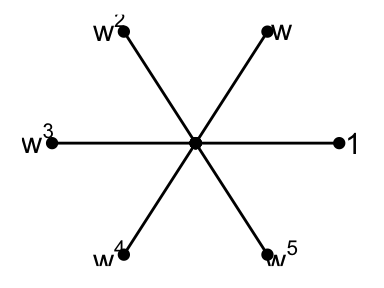
\includegraphics{t-algebra_files/figure-latex/unnamed-chunk-5-1} \end{center}

\end{example}

\textbf{Note 1.}
The symmetric group \(S_N\) acts on \(\Omega\). \(S_N \subseteq \mathrm{Aut}(\Gamma)\) acts vertex transitively on \(\Gamma\).

\textbf{Note 2.}
\(\Gamma = J(D,N)\) is isomorphic to \(\Gamma' = J(N-D,N)\).
\begin{align}
\Gamma = (X, E) & \qquad \longrightarrow & \Gamma' = (X', E')\\
X\ni S & \qquad \longmapsto & \bar{S} = \Omega\setminus S \in X'
\end{align}
This correspondence induces an isomorphism of graphs.

\emph{Pf.}
\begin{align}
ST\in E & \Leftrightarrow  |S\cap T| = D-1\\
  & \Leftrightarrow  |\Omega - (S\cup T)| = N-D-1\\
  & \Leftrightarrow  |\bar{S} \cap \bar{T}| = N-D-1\\
  & \Leftrightarrow  \bar{S}\bar{T} \in E'
\end{align}

Hence, without loss of generality, assume
\[D\leq N/2 \quad \text{for} \quad J(D,N).\]

We will need the eigenvalues of \(J(D,N)\) for certain problem later in the course. We can get these eigenvalues from our study of \(H(D,2)\).

\begin{lemma}
\protect\hypertarget{lem:ev-johnson}{}\label{lem:ev-johnson}The eigenvalues for \(J(D,N)\) with \(1\leq D \leq N/2\) are give by
\begin{align}
\theta_i & = (N-D-i)(D-i) - i \quad (0\leq i\leq D),\\
m_i & = \binom{N}{i} - \binom{N}{i-1}.
\end{align}
\end{lemma}

\begin{proof}
Let
\begin{align}
\Gamma_J & \equiv J(D,N) = (X_J, E_J)\\
\Gamma_H & \equiv H(N,2) = (X_H, E_H).
\end{align}
Set \(x \equiv 11\cdots 1 \in X_H\).

Define \(\tilde{\Gamma} \equiv (\tilde{X}, \tilde{E})\), where
\begin{align}
\tilde{X} & = \{y\in X_H \mid \partial_H(x,y) = D\} \quad \partial_H:\text{distance in }\Gamma_H\\
\tilde{E} & = \{yz\in X_H \mid \partial_H(y,z) = 2\}.
\end{align}
Observe
\begin{align}
X_J & \quad \to & \tilde{X}\\
S & \quad \mapsto & \hat{S},
\end{align}
where
\[\hat{S} = a_1\cdots a_N, \quad a_i = \begin{cases} -1 & \text{if }i\in S\\ 1 & \text{if }i\not\in S \end{cases}\]
induces an isomorphism of graphs \(\Gamma_J \to \tilde{\Gamma}\).

\emph{Pf.}
\begin{align}
ST \in E_J &\Leftrightarrow |S\cap T| = D-1\\
& \Leftrightarrow \partial_H(\hat{S}, \hat{T}) = 2\\
& \Leftrightarrow (\hat{S}, \hat{T})\in \tilde{E}.
\end{align}

Identify, \(\Gamma_J\) with \(\tilde{\Gamma}\). Then the standard module \(V_J\) of \(\Gamma_J\) becomes \(\tilde{V} = E^*_DV_H\), where \(V_H\) is the standard module of \(\Gamma_H\), and \(E^*_D \equiv E^*_D(x)\).

Let \(R\) be the raising matrix with respect to \(x\) in \(\Gamma_H\), and

let \(L\) be the lowering matrix with respect to \(x\) in \(\Gamma_H\).

Recall
\[(RL - DE^*_D) |_{\tilde{V}}\]
is the adjacency map in \(\tilde{\Gamma}\).

To find eigenvalues of \(\tilde{A}\), pick any irreducible \(T(x)\)-module \(W\) with the endpoint \(r\leq D\). Then by Theorem \ref{thm:hd2-modules}
\[\text{diam}(W) = N-2r.\]
Let \(w_0, w_1, \ldots, w_{N-2r}\) denote a basis for \(W\) as in Theorem \ref{thm:hd2-modules}. Then,
\[w_{D-r} \in E^*_DW \subseteq \tilde{V}.\]

Observe:
\begin{align}
\tilde{A}w_{D-r} & = RLw_{D-r} - DE_D^*w_{D-r}\\
& = R(N-2r-D+r+1)w_{D-r-1} - Dw_{D-r}\\
& = ((N-D-r+1)(D-r) - D)w_{D-r}.
\end{align}
Note that this is valid for \(D = r\) as well.

Hence,
\[\tilde{A}w_{D-r}  = ((N-D-r)(D-r)-r)w_{D-r}.\]
Let
\[V_H = \sum W \quad (\text{direct sum of irreducible }T(x)\text{-modules}).\]
Then,
\begin{align}
V_J & = E_D^*V_H\\
& = \sum_{W:r(W)\leq D} E_D^*W\\
& = \text{a direct sum of 1 dimensional eigenspaces for }\tilde{A}.
\end{align}
The eigenspace for eigenvalue
\[(N-D-r)(D-r)-r \quad (\text{monotonously decreasing with respec to }r)\]
appears with multiplicity
\[\binom{N}{r} - \binom{N}{r-1}\]
in this sum by Theorem \ref{thm:hd2-modules} \((iv)\).
\end{proof}

\begin{theorem}
\protect\hypertarget{thm:thin-condition}{}\label{thm:thin-condition}Let \(\Gamma = (X, E)\) be any graph. For a fixed vertex \(x\in X\), let
\[E_i^*\equiv E_i^*(x), \quad T\equiv T(x), \quad D \equiv D(x), \text{ and } K = \mathbb{C}.\]
Then we have the following implications of conditions:
\[\text{TH} \Leftrightarrow \text{C} \Leftarrow \text{S} \Leftarrow \text{G},\]
where

(TH) \(\Gamma\) is thin with respect to \(x\).

(C) \(E^*_iTE^*_i\) is commutative for every \(i\), \((0\leq i \leq D)\).

(S) \(E^*_iTE^*_i\) is symmetric for every \(i\), \((0\leq i \leq D)\).

(G) For every \(y, z\in X\) with \(\partial(x,y) = \partial(x,z)\), there exists \(g\in \mathrm{Aut}(\Gamma)\) such that

\[gx = x, \; gy = z, \; gz = y.\]
\end{theorem}

\begin{proof}
\leavevmode

(TH) \(\Rightarrow\) (C)

Fix \(i\) with \(0\leq i\leq D\). Let
\[V = \sum W. \; \text{The standard module written as a direct sum of irreducible $T$-modules}.\]
Then,
\[E_i^*V = \sum E_i^*W. \; \text{The direct sum of 1-dimensional $E_i^*TE_i^*$-modules}.\]
Since \(\dim E_i^*W = 1\), for \(a, b\in E_i^*TE_i^*\), \({ab - ba}_{| E_i^*W} = 0\). Hence \(ab - ba = 0\).

(C) \(\Rightarrow\) (TH)

Suppose \(\dim E_i^*W \geq 2\) for some irreducible \(T\)-module \(W\) with some \(i\) with \(1\leq i\leq D\).

Claim 1. \(E_i^*W\) is an irreducible \(E_i^*TE_i^*\)-module.

\emph{Proof of Claim 1.}
Suppose
\[0 \subsetneq U \subsetneq E_i^*W,\]
where \(U\) is an \(E_i^*TE_i^*\)-module. Then by the irreducibility,
\[TU = W.\]
So,
\[U \supseteq E_i^*TE_i^*U = E_i^*TU = E^*_iW.\]
This is a contradiction.

Claim 2. Each irreducible \(S = E_i^*TE_i^*\)-module \(U\) has dimension \(1\). In particular, \(\Gamma\) is thin with respect to \(x\).

\emph{Proof of Claim 2.}
Pick
\[0\neq a \in E_i^*TE_i^*.\]
Since \(\mathbb{C}\) is algebraicallt closed, \(a\) has an eigenvector \(w\in U\) with eigenvalue \(\theta\). Then,
\begin{align}
(a- \theta I)U & = (a-\theta I)Sw\\
& = S(a-\theta I)w\\
& = 0.
\end{align}
Hence,
\[a_{|U} = \theta I_{|U} \quad \text{for all }\; a\in S.\]
Thus each \(1\) dimensional subspace of \(U\) is an \(S\)-module. We have
\[\dim U = 1.\]
By Claim 1 and Claim 2, we have (TH).

\end{proof}

\textbf{HS MEMO}

Claim 1 shows the following: \emph{If \(W\) is an irreducible \(T\)-module, then \(E^*_iW\) is either \(0\) or an irreducible \(E^*_iTE^*_i\)-module.}

\hypertarget{lec8}{%
\chapter{Thin Graphs}\label{lec8}}

\textbf{Friday, February 5, 1993}

\begin{proof}[Proof of Theorem \ref{thm:thin-condition} continued]
\leavevmode

(S) \(\Rightarrow\) (C)

Fix \(i\) and pick \(a, b\in E_i^*TE_i^*\).

Since \(a\), \(b\) and \(ab\) are symmetric,
\[ab = (ab)^\top = b^\top a^\top = ba.\]
Hence \(E_i^*TE_i^*\) is commutative.

(G) \(\Rightarrow\) (S)

Fix \(i\) and pick \(a \in E_i^*TE_i^*\). Pick vertices \(y, z\in X\).

We want to show that
\[a_{yz} = a_{zy}.\]
We may assume that
\[\partial(x, y) = \partial(x,z) = i,\]
otherwise
\[a_{yz} = a_{zy} = 0.\]
By our assumption, there exists \(g\in G\) such that
\[g(y) = z, \quad g(z) = y, \quad g(x) = x.\]
Let \(\hat{g}\) denote the permutation matrix representing \(g\), i.e.,
\[\hat{g}\hat{y} =\widehat{g(y)} \quad \text{for all }\ y\in X, \quad \hat{y} = \begin{pmatrix}0\\\vdots \\ 1 \\\vdots \\0\end{pmatrix}\begin{matrix} \\ \\ \leftarrow y \\ \\ \text{ } \end{matrix}.\]
If \(g\in \mathrm{Aut}(\Gamma)\), then
\[\hat{g}A = A\hat{g} \quad \text{(Exercise)}.\]
Also, we have
\[\hat{g}E_j^* = E^*_j\hat{g} \quad (0\leq j\leq D),\]
since
\[\partial(x,y) = \partial(g(x), g(y)) = \partial(x, g(y)).\]
Hence, \(\hat{g}\) commutes with each element of \(T\). We have
\begin{align}
a_{yz} & = (\hat{g}^{-1}a\hat{g})_{yz}, \quad (\hat{g})_{yz} = \begin{cases} 1 & g(z) = y\\ 0 & \text{else.}\end{cases}\\
& = \sum_{y', z'}(\hat{g}^{-1})_{yy'}a_{y'z'}\hat{g}_{z'z}\\
& \quad (\text{zero except for $g^{-1}(y') = y, \; g(z) = z'$}.)\\
& = a_{g(y)g(z)}\\
& = a_{zy}.
\end{align}
This proves Theorem \ref{thm:thin-condition}.

\end{proof}

\textbf{Open Problem:}
Find all the graphs that satisfy the condition (G) for every vertex \(x\).

\(H(N, 2)\) is one example, because
\[\mathrm{Aut}\Gamma_{1\cdots 1} \simeq S_\Omega, \quad x = (1\cdots 1), \quad \Gamma_i(x) = \{\hat{S} \mid |S| = i\}.\]

Property (G) is clearly related to the distance-transitive property.

\begin{definition}
Let \(\Gamma = (X, E)\) be any graph. \(\Gamma\) with \(G\subseteq \mathrm{Aut}(\Gamma)\) is said to be distance-transitive \index{distance-transitive} (or two-point homogeneous), whenever
\[\text{for all } x, x', y, y'\in X \; \text{ with } \partial(x,y) = \partial(x',y'),\]
there exists \(g\in G\) such that
\[g(x) = x',\quad g(y) = y'.\]
(This means \(G\) is as close to being doubly transitive as possible.)
\end{definition}

\begin{lemma}
\protect\hypertarget{lem:property-g}{}\label{lem:property-g}

Suppose a graph \(\Gamma = (X, E)\) satisfies the property \textrm{(G) = (G($x$))} for every \(x\in X\). Then,

\((i)\) either\\
\(\quad (ia)\) \(\Gamma\) is vertex transitive; or\\
\(\quad (iia)\) \(\Gamma\) is bipartite \((X = X^+ \cup X^-)\) with \(X^+\), \(X^-\) each an orbit of \(\mathrm{Aut}(\Gamma)\).

\((ii)\) if \((ia)\) holds, then \(\Gamma\) is distance-transitive.

\end{lemma}

\begin{proof}
\((i)\)
Claim. Suppose \(y, z\in X\) are conneced by a path of even length. Then \(y, z\) are in the same orbit of \(\mathrm{Aut}(\Gamma)\).

\emph{Pf of Claim.}
It suffices to assume that the path has lenght \(2\), \(y \sim w\sim z\).

Now \(\partial(y,w) = \partial(w,z) = 1\). So there exits \(g\in \mathrm{Aut}(\Gamma)\) such that
\[gw = w, \quad gy = z, \quad gz = y.\]
This proves Claim.

Fix \(x\in X\). Now suppose that \(\Gamma\) is not vertex transitive, and we shall show \((ib)\).

Observe that \(X = X^+ \cup X^-\), where
\begin{align}
X^+ & = \{y\in X\mid \text{there exists a path of even length connecting $x$ and $y$}\},\\
X^- & = \{y\in X\mid \text{there exists a path of odd length connecting $x$ and $y$}\}.
\end{align}
Also, \(X^+\) is contained in an orbit \(O^+\) of \(\mathrm{Aut}(\Gamma)\), and \(X^-\) is contained in an orbit \(O^-\) of \(\mathrm{Aut}(\Gamma)\).

Now \(O^+\cap O^- = \emptyset\) (else \(O^+ = O^- = X\) and vertex transitive).
So,
\(X = O^+\), and \(X^- = O^-\).

Also \(X^+ \cup X^- = X\) is a bipartition by construction.

\((ii)\) Fix \(x, y, x', y'\) with \(\partial(x,y) = \partial(x',y')\).

By vertex transitivity, there exists an element
\[g_1\in G \text{ such that } g_1x = x'.\]
Observe that
\[\partial(x', y') = \partial(x,y) = \partial(g_1x, g_1y) = \partial(x', g_1y).\]
Hence, there exisits an element
\[g_2\in G \text{ such that } g_1x' = x', g_2y' = g_1y', g_2g_1y = y'\]
by (G(\(x'\))) property.

Set \(g = g_2g_1\). Then
\[gx = x', gy = y'\]
by construction.
\end{proof}

The following graphs \(\Gamma = (X, E)\) are vertex transitive, and satisfy the property (G(\(x\))) for all \(x\in X\).
\[J(D, N), \quad H(D, r), \quad J_q(D,N),\]
where

\(H(D,r)\):

\begin{align}
X & = \{a_1\cdots a_D\mid a_i\in F, 1\leq i\leq D\}\\
& \quad F: \text{ any set of cardinality $r$}\\
E & = \{xy\mid y, x\in X, \; \text{$x$ and $y$ differ in exactly one coordiate}\}.
\end{align}

\(J_q(D, N)\):

\begin{align}
X & = \text{the set of all $D$-dimensional subspaces of $N$-dimensional vector space over $GF(q)$.}\\
& \quad F: \text{ any set of cardinality $r$}\\
E & = \{xy\mid y, x\in X, \; \dim (x\cap y) = D-1\}.
\end{align}

The following graph is distance-transitive but does not satisify (G(\(x\))) for any \(x\in G\).

\(H_q(D,N)\):

\begin{align}
X & = \text{the set of all $D\times N$ matrices with entries in $GF(q)$}.\\
E & = \{xy\mid y, x\in X, \; \mathrm{rank}(x-y) = 1\}.
\end{align}

\textbf{HS MEMO}

\(H(D,r)\): \(G = S_r \mathrm{wr} S_D\), \(G_x = S_{r-1} \mathrm{wr} S_D\),

For \(x, y\in X\) with \(\partial(x, y) = \partial(x,z) = i\),
\begin{align}
Y = \{j\in \Omega \mid x_j\neq y_j\} & \leftrightarrow Z = \{j\in \Omega \mid x_j\neq z_j\}\\
(y_{j_1}, \ldots, y_{j_i}) & \leftrightarrow (z_{\ell_1}, \ldots, z_{\ell_i})
\end{align}

\(J(D, N)\): \(G = S_N\), \(G_x = S_D \times S_{N-D}\).

\begin{align}
X\cap Y & \leftrightarrow X \cap Z\\
(\Omega \setminus X)\cap Y & \leftrightarrow (\Omega \setminus X)\cap Z.
\end{align}

The following graph is distance-transitive but does not satisify (G(\(x\))) for any \(x\in G\).

\(J_q(D,N)\):

\[X\cap Y  \leftrightarrow X \cap Z.\]

The theory of a single thin irreducible \(T\)-module.

Let \(\Gamma = (X, E)\) be any graph.
\begin{align}
M & = \text{Bose-Mesner algebra over $K/\mathbb{C}$ generated by the adjacency matrix $A$.}\\
& = \mathrm{Span}(E_0, \ldots, E_R).
\end{align}

\(M\) acts on the standard module \(V = \mathbb{C}^{|X|}\).

Fix \(x\in X\), let
\(D \equiv D(x)\) be the \(x\)-diameter, and \(k = k(x)\) be the valency of \(x\).

\hypertarget{lec9}{%
\chapter{\texorpdfstring{Thin \(T\)-Module, I}{Thin T-Module, I}}\label{lec9}}

\textbf{Monday, February 8, 1993}

Let \(\Gamma = (X, E)\) be any graph.

\(M\): Bose-Mesner algebra over \(K/\mathbb{C}\) generated by the adjacency matrix \(A\).

\(\quad M = \mathrm{Span}(E_0, \ldots, E_R)\).

\(M\) acts on the standard module \(V = \mathbb{C}^{|X|}\).

Fix \(x\in X\), let
\(D \equiv D(x)\) be the \(x\)-diameter, and \(k = k(x)\) be the valency of \(x\).

\begin{definition}
Pick \(x\in X\) and write \(E_i^* \equiv E_i^*(x)\) and \(T \equiv T(x)\).

Let \(W\) be an irreducible thin \(T\)-module with endpoint \(r\), diameter \(d\).

Let \(a_i = a_i(W)\in \mathbb{C}\) satisfying
\[E_{r+i}^*A{E^*_{r+i}|}_{E_{r+i}^*W} = a_i1|_{E_{r+i}^*} \quad (0\leq i\leq d).\]
Let \(x_i = x_i(W)\in \mathbb{C}\) satisfying
\[E_{r+i-1}^*A{E^*_{r+i}AE^*_{r+i-1}|}_{E_{r+i-1}^*W} = x_i1|_{E_{r+i-1}^*} \quad (0\leq i\leq d).\]
\end{definition}

\begin{lemma}
\protect\hypertarget{lem:thin-module-structure}{}\label{lem:thin-module-structure}With above notation, the following hold.

\((i)\) \(a_i\in \mathbb{R} \quad (0\leq i\leq d)\).

\((ii)\) \(x_i\in \mathbb{R}^{>0} \quad (0\leq i\leq d)\).

\((iii)\) Pick \(0\neq w_0\in E^*_rW\). Set \(w_i = E^*_{r+i}A^iw_0\) for all \(i\). Then

\(\quad (iiia)\) \(w_0, w_1, \ldots, w_d\) is a basis for \(W\), \(w_{-1} = w_{d+1} = 0\).\\
\(\quad (iiib)\) \(Aw_i = w_{i+1} + a_iw_{i} + x_iw_{i-1} \quad (0\leq i\leq d)\).

\((iv)\) Define \(p_0, p_1, \ldots, p_{d+1}\in \mathbb{R}[\lambda]\) by

\[p_0 = 1, \quad \lambda p_i = p_{i+1} + a_i p_i + x_i p_{i-1} \quad (0\leq i\leq d),\quad p_{-1} = 0.\]

\(\quad (iva)\) \(p_i(A)w_0 = w_i, \quad (0\leq i\leq d+1)\).\\
\(\quad (ivb)\) \(p_{d+1}\) is the minimal polynomial of \(A|_W\).
\end{lemma}

\begin{proof}
\((i)\) \(a_i\) is an eigenvalue of a real symmetric matrix \(E_{r+i}^*AE^*_{r+i}\).

\((ii)\) \(x_i\) is an eigenvalue of a real symmetrix matrix \(B^\top B\), where
\[B = E^*_{r+i}AE^*_{r+i-1}.\]
Hence, \(x_i\in \mathbb{R}\).

Since \(B^\top B\) is positive semidefinite,
\[x_i \geq 0.\]
\emph{Pf.} If \(B^\top Bv = \sigma v\) for some \(\sigma \in \mathbb{R}\), \(v\in \mathbb{R}^m \setminus \{0\}\), then
\[0\leq \|Bv\|^2 = v^\top B^\top Bv = \sigma v^\top v = \sigma \|v\|^2, \quad \|v\|^2 >0.\]
Hence, \(\sigma \geq 0\).

Moreover, \(x_i\neq 0\) by Lemma \ref{lem:irreducible} \((iv)\).

\((iiia)\) Observe
\[w_i = E^*_{r+i}AE^*_{r+i-1}w_{i-1} \quad (1\leq i \leq d).\]
So \(w_i \neq 0 \quad (0\leq i \leq d)\) by Lemma \ref{lem:irreducible} \((iv)\).

Hence,
\[W = \mathrm{Span}(w_0, \ldots, w_d)\]
by Lemma \ref{lem:irreducible}. \((iii)\).

\((iiib)\) We have that
\begin{align}
Aw_i & = E^*_{r+i+1}Aw_i + E_{r+i}^*Aw_i + E^*_{r+i-1}Aw_i\\
& = w_{i+1} + E^*_{r+i}AE^*_{r+i}w_i + E^*_{r+i-1}AE^*_{r+i}AE^*_{r+i-1}w_{i-1}\\
& = w_{i+1} + a_iw_{i} + x_iw_{i-1}.
\end{align}

\((iva)\) Clear for \(i=0\). Assume it is valid for \(0, \ldots, i\).
\[p_{i+1}(A)w_0 = (A-a_iI)w_i - x_iw_{i-1} = w_{i+1}.\]

\((ivb)\) By definition,
\[p_{d+1}(A)w_0 = 0.\]
Moreover, \(p_{d+1}(A)W = 0\) because of the following.

For every \(w\in W\), write
\begin{align}
w & = \sum_{i=0}^d \alpha_i w_i \\
& = \sum_{i=0}^d \alpha_i p_i(A)w_0 && \text{for some }\alpha_i\in\mathbb{C}\\
& = p(A)w_0 && \text{for some }p\in \mathbb{C}[\lambda].
\end{align}
Hence,
\begin{align}
p_{d+1}(A)w & = p_{d+1}(A)p(A)w_0\\
& = p(A)p_{d+1}(A)w_0\\
& = 0.
\end{align}

Note that \(p_{d+1}\) is the minimal polynomial.

\emph{Pf.}
Suppose \(q(A)W = 0\) for some \(0\neq q\in \mathbb{C}[\lambda]\) with \(\deg q < \deg p_{d+1} = d+1\).
Then,
\[q = \sum_{i=0}^d\beta_ip_i \quad \text{for some }\beta_i\in \mathbb{C}.\]
We have,
\[0  = q(A)w_0  = \sum_{i=0}^d \beta_iw_i.\]
Hence \(\beta_0 = \cdots = \beta_d = 0\) by \((iiia)\). Thus \(q = 0\), and a contradiction.
\end{proof}

\begin{corollary}
\protect\hypertarget{cor:thin-is-dualthin}{}\label{cor:thin-is-dualthin}

Let \(\Gamma\), \(W\), \(r\), \(d\) be as above. Then

\((i)\) \(W\) is dual thin, that is,

\[\dim E_iW \leq 1 \quad (1\leq i \leq d).\]

\((ii)\) \(d = |\{i \mid E_iW \neq 0\}| - 1.\)

\end{corollary}

\begin{proof}
\((i)\) Set as in Lemma \ref{lem:thin-module-structure},
\[w_i = p_i(A)w_0\in E^*_{r+i}W.\]
Then \(w_0, w_1, \ldots, w_d\) is a basis for \(W\). We have
\[W = Mw_0.\]
So,
\[E_iW = E_iMw_0 = \mathrm{Span}(E_iw_0).\]
Thus,
\[\dim E_iW = \begin{cases}1 & \text{if } E_iw_0\neq 0,\\ 0 & \text{if }E_iw_0 = 0.\end{cases}\]
In particular,
\[\dim E^*_iW \leq 1.\]

\((ii)\) Immediate as
\[\dim W = d+1.\]
This proves the lemma.
\end{proof}

\begin{lemma}
\protect\hypertarget{lem:measure-wi}{}\label{lem:measure-wi}Given an irreducible \(T(x)\)-module \(W\) with endpoint \(r = r(W)\), diameter \(d = d(W)\). Write
\[x_i = x_i(W) \; (0\leq i\leq d), \quad w_i = p_i(A)w_0\in E^*_{r+i}W \; (0\leq i\leq d), \quad 0\neq w_0 \in E^*_rW.\]
Then,
\[\frac{\|w_i\|^2}{\|w_0\|^2} = x_1x_2\cdots x_i \quad (1\leq i\leq d).\]
\end{lemma}

\begin{proof}
It suffices to show that
\[\|w_i\|^2 = x_i\|w_i\|^2 \quad (1\leq i\leq d).\]
Recall by Lemma \ref{lem:thin-module-structure} \((iiib)\) that
\[Aw_j = w_{j+1} + a_jw_j + x_jw_{j-1} \quad (0\leq j\leq d), \quad w_{-1} = w_{d+1} = 0.\]
Now observe,
\begin{align}
\langle w_{i-1}, Aw_i\rangle & = \langle w_{i-1}, w_{i+1}+ a_iw_i + x_iw_{i-1}\rangle\\
& = \overline{x_i}\|w_{i-1}\|^2\\
& = x_i\|w_{i-1}\|^2.
\end{align}
by Lemma \ref{lem:thin-module-structure} \((ii)\).
Also,
\begin{align}
\langle w_{i-1}, Aw_i\rangle & = \langle Aw_{i-1}, w_i\rangle \quad (\text{since}\; \bar{A}^\top = A)\\
& = \langle x_i + a_{i-1}w_{i-1} + x_{i-1}x_{i-2}, w_i\rangle\\
& = \|w_i\|^2.
\end{align}
This proves the lemma.
\end{proof}

\begin{definition}
\protect\hypertarget{def:measure}{}\label{def:measure}Let \(W\) be an irreducible thin \(T(x)\) module with endpoint \(r\), \(E^*_i \equiv E_i^*(x)\).

The measure \index{measure} \(m = m_W\) is the function
\[m: \mathbb{R} \to \mathbb{R}\]
such that
\[
m(\theta) = \begin{cases}\frac{\|E_iw\|^2}{\|w\|^2} & \text{where } 0\neq w \in E^*_rW\\
& \text{ if $\theta = \theta_i$ is an eigenvalue for $\Gamma$,}\\
0 & \text{if $\theta$ is not an eigenvalue for $\Gamma$.}
\end{cases}\]
\end{definition}

\hypertarget{lec10}{%
\chapter{\texorpdfstring{Thin \(T\)-Module, II}{Thin T-Module, II}}\label{lec10}}

\textbf{Wednesday, February 10, 1993}

Let \(\Gamma = (X, E)\) be any graph.

Fix a vertex \(x\in X\). Let \(E^*_i \equiv E^*_i(x)\), \(T\equiv T(x)\), the subconstituent algebra over \(\mathbb{C}\), and \(V = \mathbb{C}^{|X|}\) the standard module.

\begin{lemma}
\protect\hypertarget{lem:orthogonality}{}\label{lem:orthogonality}

With above notation, let \(W\) denote a thin irreducible \(T(x)\)-module with endpoint \(r\) and diameter \(d\). Let
\begin{align}
a_i & = a_i(W) \quad (0\leq i \leq d)\\
x_i & = x_i(W) \quad (1\leq i \leq d)\\
p_i & = p_i(W) \quad (0\leq i \leq d+1)
\end{align}
be from Lemma \ref{lem:thin-module-structure}, and measure \(m = m_W\).
Then,

\((i)\) \(p_0, \ldots, p_{d+1}\) are orthogonal with respect to \(m\), i.e.,

\[\sum_{\theta\in \mathbb{R}}p_i(\theta)p_j(\theta)m(\theta) = \delta_{ij}x_1x_2\cdots x_i \quad (0\leq i,j\leq d+1) \text{ with }\; x_{d+1}=0.\]

\(\quad (ia)\) \({\displaystyle \sum_{\theta\in \mathbb{R}}p_i(\theta)^2m(\theta) = x_1\cdots x_i \quad (0\leq i\leq d)}\).

\(\quad (iia)\) \({\displaystyle \sum_{\theta\in \mathbb{R}}m(\theta) = 1}\).

\(\quad (iiia)\) \({\displaystyle \sum_{\theta\in \mathbb{R}}p_i(\theta)^2\theta m(\theta) = x_1\cdots x_ia_i \quad (0\leq i\leq d)}\).

\end{lemma}

\begin{proof}
Pick \(0\neq w_0\in E^*_rW\). Set
\[w_i = p_i(A)w_0 \in E^*_{r+i}W.\]
Since \(E^*_iW\) and \(E^*_jW\) are orthogonal if \(i\neq j\),

\begin{align}
\delta_{ij}\|w_i\|^2 & = \langle w_i, w_j\rangle\\
& = \langle p_i(A)w_0, p_j(A)w_0\rangle\\
& = \left\langle p_i(A)\left(\sum_{\ell=0}^R E_\ell\right)w_0, p_j(A)\left(\sum_{\ell=0}^R E_\ell\right)w_0\right\rangle\\
& = \left\langle \sum_{\ell=0}^R p_i(\theta_\ell)E_\ell w_0, \sum_{\ell=0}^R p_j(\theta_\ell)E_\ell w_0\right\rangle && (\text{as } AE_j = \theta_jE_j)\\
& = \sum_{\ell=0}^R p_i(\theta_\ell)\overline{p_j(\theta_\ell)}\|E_\ell w_0\|^2\\
& \qquad\qquad (\text{as } \; p_j\in \mathbb{R}[\lambda], \quad
\theta_\ell\in \mathbb{R}, \quad m(\theta_i)\|w_0\|^2 = \|E_iw_0\|^2)\\
& = \sum_{\theta\in \mathbb{R}} p_i(\theta)p_j(\theta)m(\theta)\|w_0\|^2.
\end{align}
Now we are done by Lemma \ref{lem:measure-wi} as
\[\|w_i\|^2 = \|w_0\|^2 x_1x_2\ldots x_i.\]
For \((ia)\), set \(i = j\), and for \((ib)\), set \(i=j=0\).

\((ii)\) We have
\begin{align}
\langle w_i,Aw_i\rangle & = \langle w_i, w_{i+1} + a_iw_i + x_i w_{i-1}\rangle\\
& = \overline{a_i}\|w_i\|^2\\
& = a_i x_1\cdots x_i\|w_0\|^2, 
\end{align}
as \(a_i\in \mathbb{R}\) by Lemma \ref{lem:thin-module-structure}.

Also,
\begin{align}
\langle w_i, Aw_i\rangle & = \langle p_i(A)w_0, Ap_i(A)w_0\rangle \\
& = \left\langle p_i(A)\left(\sum_{\ell=0}^R E_\ell\right)w_0, A p_i(A)\left(\sum_{\ell=0}^R E_\ell\right)w_0\right\rangle && (\text{ as in $(i)$})\\
& = \sum_{\ell = 0}^D p_i(\theta_\ell)^2 \theta_\ell \|E_\ell w_0\|^2\\
& = \sum_{\theta\in \mathbb{R}}p_i(\theta)^2\theta m(\theta)\|w_0\|^2.
\end{align}
Thus, we have \((ii)\).
\end{proof}

\begin{lemma}
\protect\hypertarget{lem:determined-by-m}{}\label{lem:determined-by-m}With above notation, let
\(W\) be a thin irreducible \(T(x)\)-module with measure \(m\). Then \(m\) determines diameter \(d(W)\),
\begin{align}
a_i & = a_i(W) \quad (0\leq i\leq d)\\
x_i & = x_i(W) \quad (1\leq i\leq d)\\
p_i & = p_i(W) \quad (0\leq i\leq d+1).
\end{align}
\end{lemma}

\begin{proof}
Note that \(d+1\) is the number of \(\theta\in \mathbb{R}\) such that \(m(\theta)\neq 0\).
Hence \(m\) determines \(d\).

Apply \((ia)\), \((ii)\) of Lemma \ref{lem:orthogonality}.
\begin{align}
& \sum_{\theta\in\mathbb{R}}m(\theta) = 1 && p_0 =1.\\
& \sum_{\theta\in\mathbb{R}}\theta m(\theta) = a_0 && p_1 = \lambda - a_0\\
& \sum_{\theta\in\mathbb{R}}p_1(\theta)^2 m(\theta) = x_1 \\
& \sum_{\theta\in\mathbb{R}}p_1(\theta)^2\theta m(\theta) = x_1a && \to a_1\\
& \qquad p_2 = (\lambda - a_1)p_1 - x_1p_0\\
& \sum_{\theta\in\mathbb{R}}p_2(\theta)^2 m(\theta) = x_1x_2 && \to x_2\\
& \sum_{\theta\in\mathbb{R}}p_2(\theta)^2\theta m(\theta) = x_1x_2a_2 && \to a_2\\
& \qquad p_3 = (\lambda-a_2)p_2 - x_2p_1\\
& \qquad\qquad \vdots\\
& \sum_{\theta\in\mathbb{R}}p_d(\theta)^2 m(\theta) = x_1x_2\cdots x_d && \to x_d\\
& \sum_{\theta\in\mathbb{R}}p_d(\theta)^2\theta m(\theta) = x_1x_2\cdots x_da_d && \to a_d\\
& \qquad p_{d+1} = (\lambda-a_d)p_d - x_dp_{d-1}.\\
\end{align}
This proves the assertions.
\end{proof}

\begin{corollary}
\protect\hypertarget{cor:isomorphic}{}\label{cor:isomorphic}

With above notation, let
\(W\), \(W'\) denote thin irreducible \(T(x)\)-modules. The following are equivalent.

\((i)\) \(W\), \(W'\) are isomorphic as \(T\)-modules.

\((ii)\) \(r(W) = r(W')\) and \(m_W = m_{W'}\).

\((iii)\) \(r(W) = r(W')\), \(d(W) = d(W')\), \(a_i(W) = a_i(W')\) and \(x_i(W) = x_i(W')\) \(\quad (0\leq i\leq d)\).

\end{corollary}

\begin{proof}
\((i)\Rightarrow (iii)\)
Write \(r\equiv r(W)\), \(r' \equiv r(W')\), \(d \equiv d(W)\), \(d' \equiv d(W')\), \(a_i \equiv a_i(W)\), \(a_i' \equiv a_i(W')\), \(x_i \equiv x_i(W)\) and \(x_i' \equiv x_i(W')\).

Let \(\sigma: W\to W'\) denote an isomorphism of \(T\)-modules. (See Definition \ref{def:isomorphic-modules}.)

For every \(i\),
\[\sigma E^*_iW = E^*_i\sigma W = E^*_iW'.\]
So, \(r = r'\) and \(d = d'\).

To show \(a_i = a_i'\), pick \(w\in E^*_{r+i}W \setminus \{0\}\). Then,
\[E^*_{r+i}AE^*_{r+i}\sigma (W) = \sigma(E^*_{r+i}AE^*_{r+i}w) = \sigma(a_iw) = a_i\sigma(w), \]
and \(\sigma w\neq 0\). So,
\begin{align}
a_i & = \text{eigenvalue of $E^*_{r+i}AE^*_{r+i}$ on $E^*_{r+i}W$}\\
& = a_i'.
\end{align}
It is similar to show \(x = x'\).

\textbf{HS MEMO}

Pick \(w\in E^*_{r+i-1}W \setminus \{0\}\), then
\[E^*_{r+i-1}AE^*_{r+i}AE^*_{r+i-1}\sigma(W) = \sigma(E^*_{r+i-1}AE^*_{r+i}AE^*_{r+i-1}w) = x_i\sigma(w).\]
Hence, \(x_i\) is the eigenvalue of \(E^*_{r+i-1}AE^*_{r+i}AE^*_{r+i-1}\) on \(E^*_{r+i-1}W = x_i'\).

\((iii)\Rightarrow (i)\)

Pick \(0\neq w_0\in E^*_rW\), \(0\neq w_0'\in E^*_rW'\). Let \(p_i\) be in Lemma \ref{lem:thin-module-structure}, and set
\begin{align}
w_i & = p_i(A)w_0\in E^*_{r+i}W \quad (0\leq i\leq d), \\
w_i' & = p_i'(A)w_0' \in E^*_{r+i}W \quad (0\leq i\leq d).
\end{align}

Define a linear transformation,
\[\sigma: W \to W' \quad (w_i \mapsto w_i').\]
Since \(\{w_i\}\) and \(\{w_i'\}\) are bases with \(d = d'\), \(\sigma\) is an isomorphism of vector spaces.

We need to show
\[a\sigma = \sigma a \quad (\text{for all }\; a\in T).\]
Take \(a = E^*_j\) for some \(j\) \((0\leq j\leq d(x))\). Then for all \(i\), we have
\[E^*_j \sigma w_i = E^*_jw_i' = \delta_{ij}w_i',\]
\[\sigma E^*_jw_i = \delta_{ij}\sigma(w_i) = \delta_{ij}w_i'.\]
\[E^*_j \sigma w_i = \sigma E^*_jw_i?\]
Take an adjacency matrix \(A\) of \(a\). Then,
\[A\sigma w_i = Aw_i' = w_{i+1}' + a_i'w_i' + x_i'w_{i-1}' = \sigma(w_{i+1} + a_iw_i + x_iw_{i-1}) = \sigma Aw_i.\]

\((ii)\Rightarrow (iii)\) Lemma \ref{lem:determined-by-m}.

\((iii)\Rightarrow (ii)\)
Given \(d\), \(a_i\), \(x_i\), we can compute the polynomial sequence
\[p_0, p_1, \ldots, p_{d+1}\]
for \(W\).

Show \(p_0, p_1, \ldots, p_{d+1}\) determines \(m = m_W\). Set
\[\Delta = \{\theta\in \mathbb{R}\mid p_{d+1}(\theta) = 0\}.\]

Observe: \(|\Delta| = d+1\). See `An Introcuction to Interlacing'.

\(m(\theta) = 0\) if \(\theta\not\in\Delta\quad (\theta\in \mathbb{R})\). So it suffices to find \(m(\theta)\), \(\theta\in \Delta\).

By Lemma \ref{lem:orthogonality} \((i)\),
\[
\begin{cases}
\sum_{\theta\in\Delta} m(\theta)p_0(\theta) & = 1,\\
\sum_{\theta\in\Delta} m(\theta)p_1(\theta) & = 0,\\
\qquad \vdots & \\
\sum_{\theta\in\Delta} m(\theta)p_d(\theta) & = 0.
\end{cases}
\]
\(d+1\) linear equation with \(d+1\) unknowns \(m(\theta)\) (\(\theta\in \Delta\)).

But the coefficient matrix is essentially Vander Monde (since \(\deg p_i = i\)).
Hence the system is nonsingular and there are unique values for \(m(\theta)\) \((\theta\in \Delta)\).
\end{proof}

\textbf{HS MEMO}

\[\begin{pmatrix}
\theta-a_0 & -1 & \cdots & 0 & 0 \\
-x_1 & \theta - a_1  & \cdots & 0 & 0 \\
\vdots & \ddots  & \ddots & \ddots & \vdots \\
0 & 0 & \cdots & \theta-a_{d-1}  & -1\\
0 & 0 & \cdots & -x_d & \theta - a_d
\end{pmatrix}
\begin{pmatrix}
p_0(\theta)\\
\vdots\\
\vdots\\
\vdots\\
p_d(\theta)
\end{pmatrix} = 0,\]
where \(\theta\) is an eigenvalue of a diagonalizable matrix
\[
L = 
\begin{pmatrix}
a_0 & 1 & \cdots & 0 & 0 \\
x_1 & a_1  & \cdots & 0 & 0 \\
\vdots & \ddots  & \ddots & \ddots & \vdots \\
0 & 0 & \cdots & a_{d-1}  & 1\\
0 & 0 & \cdots & x_d & \theta a_d
\end{pmatrix}
\]
with multiplicity \(\dim (\mathrm{Ker}(\theta I - L) = 1)\).

\hypertarget{lec11}{%
\chapter{\texorpdfstring{Examples of \(T\)-Module}{Examples of T-Module}}\label{lec11}}

\textbf{Friday, February 12, 1993}

Let \(\Gamma = (X, E)\) be a connected graph.

Let \(\theta_0\) be the maximal eigenvalue of \(\Gamma\), and \(\delta\) its corresponding eigenvector.
\[\delta = \sum_{y\in X}\delta_y \hat{y}.\]
Without loss of generality, we may assume that \(\delta_y\in \mathbb{R}^*\) for all \(y\in X\).

\begin{lemma}
\protect\hypertarget{lem:principal-module}{}\label{lem:principal-module}

Fix a vertex \(x\in X\). Write \(T \equiv T(x)\), \(E^*_i\equiv E^*_i(x)\).

\((i)\) \(T\delta = T\hat{x}\) is an irreducible \(T\)-module.

\((ii)\) Given any irreducible \(T\)-module \(W\), the following are equivalent:\\
\(\quad (iia)\) \(W = T\delta\).\\
\(\quad (iib)\) The diameter \(d(W) = d(x)\).\\
\(\quad (iic)\) The endpoint \(r(W) = 0\).

\end{lemma}

\begin{proof}
\((i)\) Observe: there exists an irreducible \(T\)-module \(W\) that contains \(\delta\).

Let \(V = \sum_{i}W_i\) be a direct sum decomposition of the standard module. Then
\[\mathrm{Span}(\delta) = E_0V = \sum_{i}E_0W_i.\]
So, \(E_0W_i \neq 0\) for some \(i\). Then,
\[\delta \in E_0W_i \subseteq W_i.\]
Observe: \(T\delta\) is an irreducible \(T\)-module.

Since \(\delta\in W\), where \(W\) is a \(T\)-module. As \(T\delta \subseteq W\) and \(W\) is irreducible, \(T\delta = W\).

Observe: \(T\delta = T\hat{x}\).

Since \(\hat{x} = \delta_x^{-1}E^*_0\delta \in T\delta\), \(T\hat{x} \subseteq T\delta\). Since \(T\delta\) is irreducible, \(T\hat{x} = T\delta\).

\((ii)\) \((a)\to (b)\):
\[E^*_i\delta = \sum_{y\in X, \partial(x,y) = i}\delta_y\hat{y} \neq 0, \quad (0\leq i\leq d(x)), \]
because \(\delta_y >0\) for every \(y\in X\).

Hence,
\[E^*_iT\delta \neq 0, \quad (0\leq i\leq d(x)).\]
Thus, \(d(x) = d(W)\).

\((b)\to (c)\): Immediate.

\((c)\to (a)\):
Since \(r(W) = 0\), \(E^*_0W \neq 0\).
Hence, \(\hat{x}\in W\) and \(T\hat{x} \subseteq W\).

By the irreduciblity, we have \(T\hat{x} = W\).
\end{proof}

\begin{lemma}
\protect\hypertarget{lem:baiparite-principal}{}\label{lem:baiparite-principal}Assume \(\Gamma\) is bipartite \((X = X^+ \cup X^-)\) (\(X^+\) and \(X^-\) are nonempty). Then the following are equivalent.

\((i)\) There exist \(\alpha^+\) and \(\alpha^-\in \mathbb{R}\) such that

\[\delta_x = \begin{cases} \alpha^+ & \text{if }\: x\in X^+\\
\alpha^- & \text{if } x\in X^-.
\end{cases}\]

\((ii)\) There exist \(k^+\) and \(k^-\in \mathbb{Z}^{>0}\) such that

\[k(x) = \begin{cases} k^+ & \text{if }\: x\in X^+\\
k^- & \text{if } x\in X^-.
\end{cases}\]
In this xase, \(k^+k^- = \theta_0^2\), and \(\Gamma\) is called bi-regular.
\end{lemma}

\begin{proof}
\((i)\to(ii)\)

\begin{center}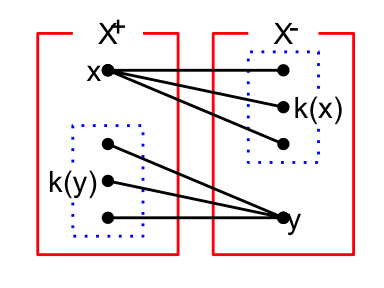
\includegraphics{t-algebra_files/figure-latex/bipartite-1} \end{center}

\begin{align}
A\delta & = A\left(\alpha^+\sum_{x\in X^+}\hat{x} + \alpha^-\sum_{y\in X^-}\hat{y}\right)\\
& = \alpha^+\sum_{y\in X^-}k(y)\hat{y} + \alpha^-\sum_{x\in X^+}k(x)\hat{x}\\
& = \theta_0\delta.
\end{align}
So,
\[k(x)\alpha^- = \theta_0\alpha^+, \quad k(y)\alpha^+ = \theta_0\alpha^-.\]
As \(\alpha^+\neq 0\) and \(\alpha^- \neq 0\),
\begin{align}
k^+ & := k(x) \; \text{ is independent of the choice of $x\in X^+$, and}\\
k^- & := k(y) \; \text{ is independent of the choice of $y\in X^-$.}
\end{align}
Moreover, \(k^+k^- = \theta_0^2\).

\((ii)\to(i)\)
Set
\[\delta' = \sum_{y\in X}\alpha_y\hat{y} \quad \text{where}\; \alpha = \begin{cases} 1/\sqrt{k^-} & \text{if }\; y\in X^+\\ 1/\sqrt{k^+} & \text{if }\; y\in X^-.\end{cases}\]
Then one checks
\begin{align}
A\delta' & = A\left(\frac{1}{\sqrt{k^-}}\sum_{y\in X^+}\hat{y} + \frac{1}{\sqrt{k^+}}\sum_{y\in X^-}\hat{y}\right)\\
& =  \frac{k^-}{\sqrt{k^-}}\sum_{y\in X^-}\hat{y} + \frac{k^+}{\sqrt{k^+}}\sum_{y\in X^+}\hat{y}\\
& = \sqrt{k^+k^-}\delta'
\end{align}
Since \(\delta' >0\), \(\delta'\in \mathrm{Span}(\delta)\), and \(\theta_0 = \sqrt{k^+k^-}\).
\end{proof}

\begin{definition}
\protect\hypertarget{def:distance-regular}{}\label{def:distance-regular}For any graph \(\Gamma = (X, E)\), fix a vertex \(x\in X\). Set \(d = d(x)\).

\(\Gamma\) is distance-regular \index{distance-regular} with respect to \(x\), if for all \(i\) : \((0\leq i\leq d)\), and all \(y\in X\) such that \(\partial(x,y) = i\):
\begin{align}
c_i(x) & := |\{z\in X \mid \partial(x,z) = i-1, \; \partial(y,z) = 1\}|,\\
a_i(x) & := |\{z\in X \mid \partial(x,z) = i, \; \partial(y,z) = 1\}|,\\
b_i(x) & := |\{z\in X \mid \partial(x,z) = i+1, \; \partial(y,z) = 1\}|
\end{align}
depends only on \(i\), \(x\), and not on \(y\).

(In this case, \(c_0(x) = a_0(x) = b_d(x) = 0\), \(c_1(x) = 1\), \(b_0(x) = k(x)\) is the valency of \(x\).)

We call \(c_i(x)\), \(a_i(x)\) and \(b_i(x)\) the intersection numbers with respect to \(x\).
\end{definition}

\begin{example}
\leavevmode

\begin{center}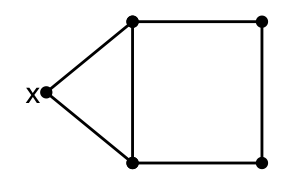
\includegraphics{t-algebra_files/figure-latex/unnamed-chunk-6-1} \end{center}

\begin{align}
c_0 &= 1, & c_1 &= 1, & c_2 &= 1,\\
a_0 &= 0, & a_1 &= 1, & a_2 &= 1,\\
b_0 &= 2, & b_1 &= 1, & b_2 &= 0.
\end{align}

\end{example}

\hypertarget{lec12}{%
\chapter{Distance-Regular}\label{lec12}}

\textbf{Monday, February 15, 1993}

\begin{lemma}
\protect\hypertarget{lem:distance-reguarity}{}\label{lem:distance-reguarity}

For any connected graph \(\Gamma = (X, E)\), the following are equivalent.

\((i)\) The trivial \(T(x)\)-module is thin for all \(x\in X\).

\((ii)\) \(\displaystyle{\left\{\sum_{y\in X, \partial(x,y) = i}\hat{y} \left| 0\leq i\leq d(x)\right.\right\}}\) is a basis for the trivial \(T(x)\)-module for every \(x\in X\).

\((iii)\) \(\Gamma\) is distance-regular with respect to \(x\) for all \(x\in X\).

\end{lemma}

\textbf{Note.}
Let \(\Gamma = (X, E)\) be a graph, with \(X = \{x, y_1, y_2, y_3, z_1, z_2, z_3\}\), \(E = \{xy_1, xy_2, xy_3, y_1z_1, y_1z_2, y_2z_3, y_3z_3\}\).

\begin{center}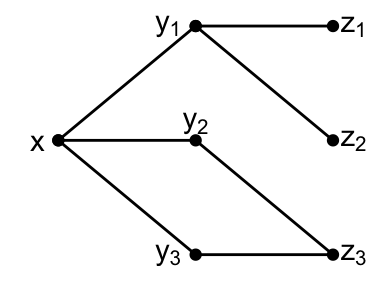
\includegraphics{t-algebra_files/figure-latex/nondr-1} \end{center}

Then \((i)\), \((ii)\) are not equivalent for a single vertex \(x\).
\begin{align}
E^*_0T\hat{x} & = \langle \hat{x}\rangle, \\
E^*_1T\hat{x} & = \langle \hat{y}_1 + \hat{y}_2 + \hat{y}_3\rangle, \\
E^*_2T\hat{x} & = \langle \hat{z}_1 + \hat{z}_2 + 2\hat{z}_3\rangle.
\end{align}

\begin{proof}[Proof of Lemma \ref{lem:distance-reguarity}]
\((i)\to (ii)\)
Let \(\delta = \sum_{y\in X}\delta_y\hat{y}\) be an eigenvector for the maximal eigenvalue \(\theta_0\). Then,
\begin{align}
\sum_{y\in X, \partial(x,y) = 1}\hat{y} & = A\hat{x} \in T(x)\hat{x} = T(x)\delta \ni E^*_1\delta\\
& = \sum_{y\in X, \partial(x,y)=1}\delta_h\hat{y}
\end{align}
If the trivial \(T(x)\)-module is thin,
\[\delta_y = \delta_z \; \text{ for }\; y, z\in X, \; \partial(x,y) = \partial(x,z) = 1.\]
Hence, \(\delta_y = \delta_z\) if \(y\) and \(z\) in \(X\) are connected by a path of even length.

So, \(\Gamma\) is regular or bipartite biregular by Lemma \ref{lem:baiparite-principal}.

In particular, \(\delta_y = \delta_z\) if \(\partial(x,y) = \partial(x,z)\), as there is a path of length \(2\cdot \partial(x,y)\);
\[y\sim \cdots \sim x \sim \cdots \sim z.\]
Hence,
\[E^*_i\delta \in \mathrm{Span}\left(\sum_{y\in X, \partial(x,y) = i}\hat{y}\right).\]
Since \(E^*_0\delta, E^*_1\delta, \ldots, E^*_d\delta\) form a basis for \(T(x)\delta\), we have \((ii)\).

\((ii)\to (iii)\)
Fix \(x\in X\), and let \(T \equiv T(x)\), \(E^*_i\equiv E^*_i(x)\), and \(d \equiv d(x)\).

\begin{align}
A\sum_{y\in X, \partial(x.y)=i}\hat{y} & = \sum_{z\in X} |\{y\in X \mid \partial(y,z) = 1, \; \partial(x,y) = i\}|\hat{z}\\
& = \sum_{z\in X, \partial(x,z) = i-1}b_{i-1}(x,z)\hat{z} \\
& \qquad + \sum_{z\in X, \partial(x,z) = i} a_{i}(x,z)\hat{z} \\
& \qquad + \sum_{z\in X, \partial(x,z) = i+1} c_{i+1}(x,z)\hat{z}\\
& \in \mathrm{Span}\left\{\left.\sum_{z\in X, \partial(x,z) = j}\hat{z} \; \right| \; j = 0, 1, \ldots, d \right\}.
\end{align}

Hence, \(b_{i-1}(x,z)\), \(a_i(x,z)\) and \(c_{i+1}(x,z)\) depend only on \(i\) and \(x\), and not on \(z\).
Therefore, \(\Gamma\) is distance-regular with respect to \(x\).

\((iii)\to (i)\)
Fix \(x\in X\), and let \(T \equiv T(x)\), \(E^*_i\equiv E^*_i(x)\), and \(d \equiv d(x)\).
By defintion of distance-regularity, for every \(i\) \((0\leq i\leq d)\),
\begin{align}
A\left(\sum_{y\in X, \partial(x,y)=i}\hat{y}\right) & = 
b_{i-1}(x)\sum_{y\in X, \partial(x,y) = i-1}\hat{y} \\
& \qquad + a_{i}(x)\sum_{y\in X, \partial(x,y) = i}\hat{y}\\
& \qquad + c_{i+1}(x)\sum_{y\in X, \partial(x,y) = i+1}\hat{y}.
\end{align}
Hence,
\[W = \mathrm{Span}\left\{\left.\sum_{y\in X, \partial(x,y)=i}\hat{y} \; \right| \; 0\leq i\leq d\; \right\}\]
is \(A\)-invariant and so \(T\)-invariant. Since \(\hat{x}\in W\), \(T\hat{x} = W\) is the trivial module and \(T\hat{x}\) is thin.
\end{proof}

Next, we show more is true if \((i)-(iii)\) hold in Lemma \ref{lem:distance-reguarity}.

In fact, \(d(x)\), \(a_i(x)\), \(c_i(x)\), and \(b_i(x)\) are
\[\begin{cases} 
\text{independent of $X$} & \text{if $\Gamma$ is regular; or}\\
\text{constant over $X^+$ and $X^-$} & \text{if $\Gamma$ is biregular.}
\end{cases}\]

Let \(\Gamma = (X, E)\) be any (connected) graph. Pick vertices \(x, y\in X\).

Let \(W\) be a thin, irreducible \(T(x)\)-module, and
measure \(m: \mathbb{R} \to \mathbb{R}\) determined by \(W\).

Let \(W'\) be a thin, irreducible \(T(y)\)-module, and
measure \(m: \mathbb{R} \to \mathbb{R}\) determined by \(W'\).

Recall \(W\), \(W'\) are orthogonal if
\[\langle w, w'\rangle = 0 \quad \text{for all }w\in W, w'\in W'.\]

We shall show if \(W\) and \(W'\) are note orthogonal, then \(m\) and \(m'\) are related:
\[m\cdot \mathrm{poly}_1 = m'\cdot \mathrm{poly}_2\]
for some polynomials with
\[\deg \mathrm{poly}_1 + \deg \mathrm{poly}_2 \leq 2\cdot \partial(x,y).\]

\textbf{Notation.}
\(V\): standard module of \(\Gamma\).

\(H\): any subspace of \(V\).

\[V = H + H^\bot \quad \text{orthogonal direct sum},\]
and for \(v = v_1 + v_2\) \(\mathrm{proj}_H: V\to H \; (v\mapsto v_1)\): linear transformation.

Observe:
For every \(v\in V\),
\[v - \mathrm{proj}_H v \in H^\bot.\]
So,
\[\langle v - \mathrm{proj}_H v, h\rangle = 0 \quad \text{for all }\;h\in H \text{ or},\]
\[\langle v, h\rangle = \langle \mathrm{proj}_H v, h\rangle \quad \text{for all }\;v\in V, \;\text{ and for all }\: h\in H.\]

\begin{theorem}
\protect\hypertarget{thm:two-thin-modules}{}\label{thm:two-thin-modules}Let \(\Gamma = (X,E)\) be any graph. Pick vertices \(x,y\in X\) and set \(\Delta = \partial(x,y)\). Assume

\(W\): thin irreducible \(T(x)\)-module with endpoint \(r\), diameter \(d\), and measure \(m\).

\(W'\): thin irreducible \(T(y)\)-module with endpoint \(r'\), diameter \(d'\), and measure \(m'\).

\(W\) and \(W'\) are not orghotonal.

Now pick
\[0\neq w\in E^*_r(x)W, \quad 0\neq w\in E^*_{r'}(x)W'.\]
Then,

\((i)\) \({\displaystyle \mathrm{proj}_{W'}w = p(A)\frac{\|w\|}{\|w'\|}w'}\)

for some \(0\neq p\in \mathbb{C}[\lambda]\) with \(\deg p \leq \Delta - r' + r, d'\),

\({\displaystyle \mathrm{proj}_{W}w' = p'(A)\frac{\|w'\|}{\|w\|}w}\)

for some \(0\neq p'\in \mathbb{C}[\lambda]\) with \(\deg p \leq \Delta - r + r', d\).

\((ii)\) For all eigenvalues \(\theta_i\) of \(\Gamma\),

\[\frac{\langle E_iw, E_iw'\rangle}{\|w\|\|w'\|} = m(\theta_i)\overline{p'(\theta_i)}.\]

\((iii)\) For all eigenvalues \(\theta_i\) of \(\Gamma\),

\[p(\theta_i)p'(\theta_i)\]
is in a real number in interval \([0,1]\).
\end{theorem}

\begin{proof}
\((i)\) Since \(W\), \(W'\) are not orthogonal, there exist
\[v\in W, \; v'\in W' \; \text{ sich that }\; \langle v, v'\rangle \neq 0.\]
Then there exists \(a\in M\) such that
\[v' = aw'.\]
(This is becase \(w'_i = p'_i(A)w_0'\) and hence for every \(v'\in W'\), there is a polynomial \(q\in \mathbb{C}[\lambda]\), \(q(A)w_0' = v\).)

We have
\[0\neq \langle v', v\rangle = \langle aw', v\rangle = \langle w', a^*v\rangle\]
and \(a^*v\in W\).

Hence, \(\mathrm{proj}_{W} w' \neq 0\).

Let \(p_0, \ldots, p_d\in \mathbb{C}[\lambda]\) be from Lemma \ref{lem:thin-module-structure}.

Then, \(w_i = p_i(A)w\) is a basis for \(E^*_{r+i}(x)W \quad (0\leq i\leq d)\).

Hence,
\[\mathrm{proj}_{W}w' = \alpha_0w_0 + \cdots + \alpha_dw_d \quad \text{for some }\; \alpha_j\in \mathbb{C}.\]
Set
\[p' := \frac{\|w\|}{\|w'\|}\sum_{i=0}^d \alpha_ip_i.\]
Then \(0\neq p'\in \mathbb{C}[\lambda]\) and \(\deg p' \leq d\).

Claim: \(\alpha_i = 0\) \((\Delta - r + r' < i\leq d)\).

In particular, \(\deg p' \leq \Delta - r + r'\).

\emph{Pf.} Obseve:
\[w'\in E^*_{r'}(y)V, \quad w \in E^*_r(x)V,\]
for \(\partial(x,y) = \Delta\).
\[E^*_{r'}(y)V \cap E^*_{r+i}(x)V = 0\]
by triangle inequality.

(\(\Delta = \partial(x,y) < r+i - r'\) or \(\Delta + r' < r + i\) by our choice of \(i\).)

\begin{center}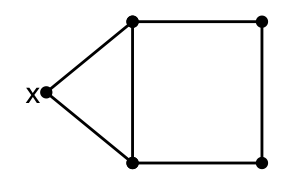
\includegraphics{t-algebra_files/figure-latex/unnamed-chunk-7-1} \end{center}

Hence,
\[E^*_{r'}(y)V \bot E^*_{r+i}(x)V,\]
or
\begin{align}
0 & = \langle w', w_i\rangle \\
& = \langle \mathrm{proj}_{W}w', w_i\rangle\\
& = \sum_{j=0}^d\alpha_j\langle w_j, w_i\rangle\\
& = \alpha_i\|w_i\|^2.
\end{align}
Hence, \(\alpha_i = 0\).
Thus,
\begin{align}
\mathrm{proj}_{W}w' & = \sum_{i=0}^{\Delta + r' - r}\alpha_iw_i\\
& = \sum_{i=0}^{\Delta + r' - r}\alpha_ip_i(A)w_0\\
& = p'(A)\frac{\|w'\|}{\|w\|}w.
\end{align}

\((ii)\) We have
\begin{align}
\frac{\langle E_iw, E_iw'\rangle}{\|w\|\|w'\|}
& = \frac{\langle E_iw, w'\rangle}{\|w\|\|w'\|}\\
& = \frac{\langle E_iw, \mathrm{proj}_W w'\rangle}{\|w\|\|w'\|} && \text{as }\; \mathrm{proj}_Ww' = p'(A)\frac{\|w\|}{\|w'\|}w\\
& = \frac{\langle E_iw, p'(A) w\rangle}{\|w\|^2}\\
& = \frac{\langle E_iw, E_ip'(A) w\rangle}{\|w\|^2}\\
& = \overline{p'(\theta_i)}\frac{\|E_iW\|^2}{\|w\|^2}\\
& = \overline{p'(\theta_i)}m(\theta_i).
\end{align}
Moreover, as \(m(\theta_i)\), \(m'(\theta_i)\in \mathbb{R}\),
\[\frac{\langle E_iw, E_iw'\rangle}{\|w\|\|w'\|}  = \frac{\overline{\langle E_iw, E_iw'\rangle}}{\|w'\|\|w\|}
 = \overline{\overline{p(\theta_i)}m'(\theta_i)} 
 = p(\theta_i)m'(\theta_i).\]

\((iii)\) Sicne,
\[\frac{|\langle E_iw, E_iw'\rangle\|^2}{\|w\|^2\|w'\|^2} = p(\theta_i)p'(\theta_i)m(\theta_i)m'(\theta_i),\]
\begin{align}
p(\theta_i)p'(\theta_i) & = \frac{|\langle E_iw, E_iw'\rangle\|^2}{m(\theta_i)m'(\theta_i)\|w\|^2\|w'\|^2} \in \mathbb{R}\\
& = \frac{|\langle E_iw, E_iw'\rangle\|^2}{\frac{\|E_iw\|^2}{\|w\|^2}\frac{\|E_iw'\|^2}{\|w'\|^2}\|w\|^2\|w'\|^2}.
\end{align}

By Cauchy-Schwartz inequality,
\[(|\langle a, b\rangle | \leq \|a\|\|b\|,)\]
\[\frac{|\langle E_iw, E_iw'\rangle\|^2}{\|E_iw\|^2\|E_iw'\|^2} \leq 1.\]
Hence, we have the assertion.
\end{proof}

\hypertarget{lec13}{%
\chapter{Modules of a DRG}\label{lec13}}

\textbf{Wednesday, February 17, 1993}

\begin{lemma}
\protect\hypertarget{lem:two-principal-modules}{}\label{lem:two-principal-modules}Let \(\Gamma = (X, E)\) be any graph. Pick an edge \(xy\in E\).

Assume the trivial \(T(x)\)-module \(T(x)\delta\) is thin with measure \(m_x\),

and the trivial \(T(y)\)-module \(T(y)\delta\) is thin with measure \(m_y\).

Then,

\((ia)\) \({\displaystyle \frac{m_x(\theta)}{k_x} = \frac{m_y(\theta)}{k_y} \text{ for all } \theta\in \mathbb{R}\setminus \{0\}}\).

\((ib)\) \({\displaystyle \frac{m_x(0) -1}{k_x} = \frac{m_y(0)-1}{k_y} \text{ for all } \theta\in \mathbb{R}\setminus \{0\}}\).

\[(\delta = \sum_{y\in X}\delta_y \hat{y} \quad \text{eigenvector corresponding to the maximal eigenvalue})\]
\end{lemma}

\begin{proof}
Apply Theorem \ref{thm:two-thin-modules},
\begin{align}
W & = T(x)\delta \quad r = 0, \quad d = d(x)\\
W' & = T(y)\delta \quad r' = 0, \quad d' = d(y).
\end{align}
Take \(w = \hat{x}\), \(w' = \hat{y}\).

Claim. \(\mathrm{proj}_{T(y)\delta}\hat{x} = k^{-1}_yA\hat{y}\).

\emph{Pf.}
Since
\[\hat{y}\in T(y)\delta, \quad A\hat{y}\in T(y)\delta.\]
Show
\[(\hat{x} - {k_y}^{-1} A\hat{y}) \bot (T(y)\delta).\]
Recall
\[A\hat{y} = \sum_{z\in X, yz\in E}\hat{z}.\]
\[\hat{x} - {k_y}^{-1}Ay \in E^*_1(y)V.\]
So,
\[\hat{x} - \frac{1}{k_y}A\hat{y} \; \bot \; E^*_j(y)T(y)\delta \quad \text{if $j\neq 1$}\; (0\leq j\leq k(y)).\]
And we have,
\begin{align}
\left\langle \hat{x} - \frac{1}{k_y}A\hat{y}, A\hat{y}\right\rangle
& = \left\langle \hat{x}, \sum_{z\in X, yz\in E}\hat{z}\right\rangle - \frac{1}{k_y}\left\|\sum_{z\in X, yz\in E}\hat{z}\right\|^2\\
& =  1 - 1\\
& = 0
\end{align}
This proves Claim.

Similarly,
\[\mathrm{proj}_{T(x)\delta}\hat{y} = {k_x}^{-1}A\hat{x}.\]
Hence, the polynomials \(p, p'\in \mathbb{C}[\lambda]\) from Theorem \ref{thm:two-thin-modules} equal
\[\frac{\lambda}{k_y} \quad \text{ and }\quad \frac{\lambda}{k_x}\]
respectively.

By Theorem \ref{thm:two-thin-modules},
\[\frac{m_x(\theta)\theta}{k_x} = m_x(\theta)\overline{p'(\theta)} = m_y(\theta)\overline{p(\theta)} = \frac{m_y(\theta)\theta}{k_y}.\]
If \(\theta\neq 0\), we have \((ia)\).

Also,
\begin{align}
\frac{1-m_x(0)}{k_x} & = \left(\sum_{\theta\in \mathbb{R}\setminus \{0\}}m_x(0)\right)\frac{1}{k_x} && \text{by $(ia)$}\\
& = \left(\sum_{\theta\in \mathbb{R}\setminus \{0\}}m_y(0)\right)\frac{1}{k_y}\\
& = \frac{1 - m_y(0)}{k_y}
\end{align}
Hence, we have \((ib)\).
\end{proof}

\begin{theorem}
\protect\hypertarget{thm:distance-regular-x}{}\label{thm:distance-regular-x}Suppose any graph \(\Gamma = (X, E)\) is distance-regular with respect to every vertex \(x\in X\).
(So \(\Gamma\) is regular or biregular by Lemma \ref{lem:distance-reguarity}.)

Then,

Case \(\Gamma\) is regular: the diameter \(d(x)\) and the intersection numbers \(a_i(x)\), \(b_i(x)\), \(c_i(x)\) \((0\leq i\leq d(x))\) are independent of \(x\in X\).

(And \(\Gamma\) is called distance-regular.)

Case \(\Gamma\) is biregular: \((X = X^+\cup X^-)\)

\(d(x)\) and \(a_i(x)\), \(b_i(x)\), \(c_i(x)\) \((0\leq i\leq d(x))\) are constant over \(X^+\) and \(X^-\).
(And \(\Gamma\) is called distance-biregular.)
\end{theorem}

\begin{proof}
We apply Lemma \ref{lem:two-principal-modules}.

Case \(\Gamma\): regular.

Then \(m_x = m_y\) for all \(xy\in E\). Hence, the measure of the trivial \(T(x)\)-module is independent of \(x\in X\).

Case \(\Gamma\) is biregular.

Then \(m_x = m_{x'}\) for all \(x, x'\in X\) with \(\partial(x,x') = 2\).

Hence, the measure of the trivial \(T(x)\)-module is constant over \(x\in X^+\), \(X^-\).

Fix \(x\in X\). Write \(T\equiv T(x)\), \(E^*_i \equiv E^*_i(x)\), \(W = T\delta\) with measure \(m\), diameter \(d = d(x)\).

We know by Corollary \ref{cor:isomorphic} that \(m\) determines
\[d, \quad a_i(W) \; (0\leq i\leq d), \quad x_i(W) \; (1\leq i\leq d)\]
(as \(d = D(x) = d(W)\) by Lemma \ref{lem:principal-module}.)

We shall show that \(m\) determines
\[a_i(x), \;  c_i(x), \; b_i(x) \quad (0\leq i\leq d).\]
Observe:
\begin{align}
a_i(W) & = a_i(x) \quad (0\leq i\leq d)\\
x_i(W) & = b_{i-1}(x)c_i(x) \quad (1\leq i\leq d)
\end{align}

\textbf{HS MEMO}

\(a_i = a_i(W)\) is an eigenvalue of
\[E^*_iAE^*_i \text{ on } E^*_iW = \langle \sum_{y\in \Gamma_i(x)}\hat{y}\rangle. \]
(See Lemma \ref{lem:distance-reguarity}.)

\(x_i = x_i(W)\) is an eigenvalue of
\[E^*_{i-1}AE^*_iAE^*_{i-1} \text{ on } E^*_{i-1}W,\]
and
\begin{align}
A\sum_{y\in X,\partial(x,y)}\hat{y} & = b_{i-1}(x)\sum_{y\in X, \partial(x,y)=i-1}\hat{y} \\
& \quad + a_i(x)\sum_{y\in X, \partial(x,y)=i}\hat{y} \\
& \quad + c_{i+1}(x)\sum_{y\in X, \partial(x,y)=i+1}\hat{y}
\end{align}
So \(x_i = b_{i-1}(x)c_i(x)\).

Set \(k^+ = k_x\). Define
\[k^- = \frac{{\theta_0}^2}{k^+},\]
where \(\theta_0\) is the maximal eigenvalue. (See Lemma \ref{lem:principal-module}.)

(So, \(k^+ = k^-\) is the valency, if \(\Gamma\) is regular.)

For every \(i \; (0\leq i\leq d)\) and for every \(z\in X\) with \(\partial(x,z) = i\),
\begin{align}
k_z & = c_i(x) + a_i(x) + b_i(x)\\
& = \begin{cases} k^+ & \text{if $i$ is even,}\\
k^- & \text{ if $i$ is odd.}
\end{cases}
\end{align}

Now \(m\) determines
\[c_0(x) = a_0(x) = 0,\quad c_1(x) = 1,\]
\[b_0(x) = b_0(x)c_1(x) = x_1(W).\]
\begin{align}
k^+ & = b_0(x)\\
k^- & = {\theta_0}^2/k^+\\
c_i(x) & = x_i(W)/b_{i-1}(x) \quad (1\leq i\leq d)\\
b_i(x) & = \begin{cases} k^+ - a_i(x) - c_i(x) \quad \text{$i$; even,}\\
k^--a_i(x)-c_i(x) \quad \text{$i$: odd}.
\end{cases}
\end{align}
This proves the assertions.
\end{proof}

\begin{proposition}
\protect\hypertarget{prp:dim-diameter}{}\label{prp:dim-diameter}

Under the assumption of Theorem \ref{thm:distance-regular-x}, the following hold.

Case \(\Gamma\): regular.

\((i)\) \(\dim E_iV = |X|m(\theta_i)\).\\
\((ii)\) \(\Gamma\) has exactly \(d+1\) distinct eigenvalues

(\(d = \mathrm{diam}\Gamma = d(x), \; \text{ for all }\; x\in X\)).

Case \(\Gamma\): biregular.

\((i)\) \(\dim E_iV = |X^+| m^+(\theta_i) + |X^-|m^-(\theta_i)\).\\
\((ii)\) \(\Gamma\) has exactly \(d^++1\) distinct eigenvalues \((d^+\geq d^-)\).\\
\((iii)\) If \(d^+\) is odd, the \(\Gamma\) is regular.\\
\((iv)\) \(d^+ = d^-\), or \(d^+ = d^-+1\) is even.\\
\((v)\) \(a_i(x) = 0\) for all \(i\) and for all \(x\).

\end{proposition}

\begin{proof}

\((i)\) Suppose \(\Gamma\) is regular.

Let \(m_x\) be the measure of the trivial \(T(x)\)-module,
\[m_x(\theta_i) = \|E_i\hat{x}\|^2, \quad \text{as}\; \|\hat{x}\| = 1.\]
Now,
\begin{align}
|X|m_x(\theta_i) & = \sum_{x\in X}m_x(\theta_i)\\
& = \sum_{x\in X}\|E_i\hat{x}\|^2\\
& = \sum_{y,z\in X}|(E_i)_{yz}|^2\\
& = \mathrm{trace} E_i\overline{E_i}^\top.
\end{align}
Since \(A\) is real symmetric and
\[E_i\overline{E_i}^\top = E_i^2 = E_i\]
with \(E_i\) symmetric
\[E_i \sim \begin{pmatrix} I & O \\ O & O\end{pmatrix}.\]
\[\mathrm{trace} E_i = \mathrm{rank} E_i = \dim E_iV.\]
Thus, we have the assertion in this case.

Suppose \(\Gamma\) is biregular.

Then, same except,
\[\sum_{x\in X} m_x(\theta_i) = |X^+|m^+(\theta_i) + |X^-|m^-(\theta_i).\]

\((ii)\)
\(\Gamma\): regular. Immediately, if \(\theta\) is an eigenvalue of \(\Gamma\), then \(m(\theta) \neq 0\).

\(\Gamma\): biregular. For each \(\theta = \theta_i \in \mathbb{R}\setminus\{0\}\),
\begin{align}
m^-(\theta) \neq 0 &\Leftrightarrow m^+(\theta) \neq 0\\
& \Leftrightarrow \theta \; \text{ is an eigenvalue of $\Gamma$}\\
& \quad\quad \left(\frac{m^+(\theta)}{k^+} = \frac{m^-(\theta)}{k^-} \right)
\end{align}

\((iv)\) and \((v)\) are clear.

\textbf{HS MEMO}

\((iii)\) If \(d^+\) is odd, \(d^+ = d^-\) and \(\Gamma\) has even number of eigenvalues, i.e., \(0\) is not an eigenvalue.
So \(A\) is nonsingular, and \(\Gamma\) is regular.

\end{proof}

\hypertarget{lec14}{%
\chapter{Parameters of Thin Modules, I}\label{lec14}}

\textbf{Friday, February 19, 1993}

Summary.

\begin{definition}
Assume \(\Gamma = (X, E)\) is distance-regular with respect to every vertex \(x\in X\).

Notation: Let \(x\in X\). The data of the trivial \(T(x)\)-module.

\[\begin{array}{|c|c|c|}
\hline
& \text{Case DR}  & \text{Case DBR} \\
\hline
\text{valency} k_x & k & \begin{cases} k^+ & \text{ if } x\in X^+\\
k^- & \text{ if } x\in X^-\end{cases}\\
x\text{-diameter } D_x & D & \begin{cases} D^+ & \text{ if } x\in X^+\\
D^- & \text{ if } x\in X^-\end{cases}\\
\text{measure $m_x$} & m & \begin{cases} m^+ & \text{ if } x\in X^+\\
m^- & \text{ if } x\in X^-\end{cases}\\
\text{int. number }c_i(x) & c_i & \begin{cases} c_i^+ & \text{ if } x\in X^+\\
c_i^- & \text{ if } x\in X^-\end{cases}\\ 
\text{int. number }b_i(x) & b_i & \begin{cases} b_i^+ & \text{ if } x\in X^+\\
b_i^- & \text{ if } x\in X^-\end{cases}\\ 
\text{int. number }a_i(x) & a_i & 0\\ 
\hline
\end{array}\]

Call \(m\), \(m^{\pm 1}\) the measure of \(\Gamma\).
\end{definition}

Assume \(\Gamma = (X, E)\) is distance-regular.

To what extent do \(a_i\)'s, \(b_i\)'s and \(c_i\)'s determine the structure of irreducible \(T(x)\)-modules? In general, the following hold.

\begin{lemma}
\protect\hypertarget{lem:basic-data}{}\label{lem:basic-data}Assume \(\Gamma = (X, E)\) is distance-regular. Pick \(x\in X\). Let \(W\) be a thin irreducible \(T(x)\)-module with endpoint \(r\), diameter \(d\) and measure \(m_W\).

\((i)\) There is a unique polynomial \(f_W \in \mathbb{C}[\lambda]\) with the following properties.

\(\quad (ia)\) \(\deg f_W \leq D\) (diameter of \(\Gamma\)).

\(\quad (ib)\) \(m_W(\theta) = m(\theta)f_W(\theta)\) for every \(\theta\in \mathbb{R}\), where \(m\) is the measure of \(\Gamma\).

Moreover, \(f_W\in \mathbb{R}[\lambda]\), and

\((ii)\) \(\deg f_W \leq 2r\).\\
\((iii)\) For all eigenvalues \(\theta_i\) of \(\Gamma\), \(\lambda - \theta_i\) is a factor of \(f_W\) whenever, \(E_iW = 0\).

In particular, \(2r-D+d\geq 0\).
\end{lemma}

\begin{proof}
Let \(\theta_0, \ldots, \theta_D\) denote distinct eigenvalues of \(\Gamma\). Then \(m(\theta_i) \neq 0\) \((0\leq i\leq D)\) by Proposition \ref{prp:dim-diameter}.

There exists a unique \(f_W\in \mathbb{C}[\lambda]\) with \(\deg f_W\leq D\) such that
\[f_W(\theta_i) = \frac{m_W(\theta_i)}{m(\theta_i)} \quad (0\leq i\leq D)\]
by polynomial interpolation.

\(f_W\in \mathbb{R}[\lambda]\) since
\[\theta_0, \ldots, \theta_D\in \mathbb{R} \quad \text{and}\quad f_W(\theta_0), \ldots, f_W(\theta_D) \in \mathbb{R}.\]

\((ii)\) Without loss of generality, we may assume \(r < D/2\), else trivial.

Pick \(0\neq w \in E^*_r(x)W\).
\[w = \sum_{y\in W, \partial(x,y) = r}\alpha_y\hat{y} \quad \text{ for some } \; \alpha_y\in \mathbb{C}.\]
Pick \(y\in X\) such that \(\alpha_y\neq 0\).

Set \(W'\) be the trivial \(T(y)\)-module. (\(\langle w, \hat{y}\rangle \neq 0, \text{ as } W\not\bot W'\).)
\[r' = 0, \quad m' = m, \quad \Delta = r.\]

Apply Theorem \ref{thm:two-thin-modules}, we have
\begin{align}
\deg p & \leq \Delta - r' + r = 2r, \quad p\neq 0\\
\deg p' & \leq \Delta - r + r' = 0 , \quad p'\neq 0.
\end{align}
\[m_W(\theta)\overline{p'(\theta)} = m(\theta)p(\theta) \quad (\text{ for all } \theta \in \mathbb{R}).\]
So,
\[\deg p/\bar{p}' \leq 2r,\]
and \(p/\bar{p}'\) satisfies the conditions of \(f_W\).
\[\left(\frac{p(\theta)}{\bar{p}'(\theta)} = \frac{m_W(\theta)}{m(\theta)}\right)\]

\((iii)\)
\[E_iW = 0 \Rightarrow m_W(\theta_i) = 0 \Rightarrow f_W(\theta_i) = 0.\]
that is, \(E_iW = 0\). Hence \(\theta_i\) is a root of \(f_W(\lambda) = 0\).
So,
\[2r \geq \deg f_W \geq |\{\theta_i\mid E_iW = 0\}| = D-d.\]
Hence,
\[2r-D + d \geq 0.\]
This proves the assertions.
\end{proof}

\begin{lemma}
\protect\hypertarget{lem:thin-endpoint1}{}\label{lem:thin-endpoint1}Let \(\Gamma = (X, E)\) be any distance-regular graph with valency \(k\), diameter \(D\) \((d\geq 2)\), measure \(m\), and eigenvalues
\[k = \theta_0 > \theta_1 > \cdots > \theta_D.\]
Pick \(x\in X\). Let
\(W\) be a thin irreducible \(T(x)\)-module with endpoint \(r = 1\), diameter \(d\) and measure \(m_W = mf_W\).
Then one fo the following cases \((i)-(iv)\) occurs.

\[\begin{array}{|c|c|c|c|}
\hline
\text{Case} & d  & f_W(\lambda) & a_0(W) \\
\hline
(i) & D-2 & \frac{(\lambda - k)(\lambda - \theta_1)}{k(\theta_1 + 1)} & -\frac{b_1}{\theta_1 + 1} -1\\
(ii) & D-2 & \frac{(\lambda - k)(\lambda - \theta_D)}{k(\theta_D + 1)} & -\frac{b_1}{\theta_1 + 1} -1\\
(iii) & D-1 & \frac{k - \lambda}{k} & -1\\
(iv) & D-1 & \frac{(\lambda - k)(\lambda - \beta)}{k(\beta + 1)} & -\frac{b_1}{\beta + 1} -1\\ 
\hline
\end{array}\]
for some \(\beta\in \mathbb{R}\) with \(\beta\in (-\infty, \theta_D) \cup (\theta_1, \infty)\).
Moreover, the isomorphism class of \(W\) is determined by \(a_0(W)\).
\end{lemma}

\textbf{Note.} By \((iii)\), the possible ``shapes'' of a thin irreducible \(T(x)\)-modules are:
\begin{align}
r = 0 & \quad d = D,\\
r = 1 & \quad d = D-1,\\
r = 1 & \quad d = D-2.
\end{align}

\hypertarget{lec15}{%
\chapter{Parameters of Thin Modules, II}\label{lec15}}

\textbf{Monday, February 22, 1993}

\begin{proof}[Proof of Lemma \ref{lem:thin-endpoint1} Continued]
\leavevmode

We have \(\deg f_W\leq 2\) by Lemma \ref{lem:basic-data} \((ii)\).

Also by Lemma \ref{lem:principal-module}, \(E_0W = 0\).

(As otherwise \(\langle \delta \rangle = E_0V \subseteq W\) and \(r(W) = 0\).)

Hence, \(\lambda - \theta_0 = \lambda - k\) is a factor of \(f_W\) by Lemma \ref{lem:basic-data} \((iii)\).

Let \(p_0, p_1, \ldots, p_D\) denote the polynomials for the trivial \(T(x)\)-module from Lemma \ref{lem:thin-module-structure}.

Recall,
\begin{align}
\sum_{\theta\in \mathbb{R}}m(\theta)p_i(\theta)p_j(\theta) & = \delta_{ij}x_1x_2\cdots x_i \quad (0\leq i,j\leq D)\\
& = \delta_{ij}b_0b_1\cdots b_{i-1}c_1c_2\cdots c_i.
\end{align}
Note that \(x_i = b_{i-1}c_i\) is in the proof of Theorem \ref{thm:thin-condition}.

By construction,
\begin{align}
p_0(\lambda) & = 1,\\
p_1(\lambda) & = \lambda,\\
p_2(\lambda) & = \lambda^2 - a_1\lambda - k.
\end{align}

Apparently,
\[f_W = \sigma_0 p_0 + \sigma p_1 + \sigma_2 p_2\]
for some \(\sigma_0, \sigma_1, \sigma_2\in \mathbb{C}\).

Claim:
\begin{align}
\sigma_0 & = 1,\\
\sigma_1 & = \frac{a_0(W)}{k},\\
\sigma_2 & = -\frac{1+a_0(W)}{kb_1}.
\end{align}

\emph{Pf of Claim.}
\begin{align}
1 & = \sum_{\theta\in \mathbb{R}}m_W(\theta)\\
& = \sum_{\theta\in \mathbb{R}}m(\theta)f_W(\theta)\\
& = \sum_{j=0}^2 \sigma_j\left(\sum_{\theta\in \mathbb{R}}m(\theta)p_j(\theta)\right)\\
& = \sigma_0.
\end{align}
We applied Lemma \ref{lem:orthogonality} \((ib)\), Lemma \ref{lem:basic-data} \((ib)\), and Lemma \ref{lem:orthogonality} \((i)\) in this order.

Next by Lemma \ref{lem:orthogonality} \((ii)\), and \(p_1(\theta) = \theta\),
\begin{align}
a_0(W) & = \sum_{\theta\in \mathbb{R}}m_W(\theta)\theta\\
& = \sum_{\theta\in \mathbb{R}}m(\theta)f_W(\theta)\theta\\
& = \sum_{j = 0}^2\sigma_j\sum_{\theta\in \mathbb{R}}m(\theta)p_j(\theta)p_1(\theta)\\
& = \sigma_1 x_1(T\delta)\\
& = \sigma_1b_0c_1\\
& = \sigma_1 k.
\end{align}
So far,
\[f_W(\lambda) = 1 + \frac{a_0(W)}{k}\lambda + \sigma_2(\lambda^2 - a_1\lambda-k).\]
But,
\begin{align}
0 & = f_W(k)\\
& = 1 + a_0(W) + \sigma_2k(k-a_1-1)\\
& = 1 + a_0(W) + \sigma_2kb_1.
\end{align}
Thus,
\[\sigma_2 = -\frac{1+a_0(W)}{kb_1}.\]
This proves Claim.

Case: \(a_0(W) = -1\).

Here, \(\sigma_2 = 0\) and
\[f_W(\lambda) = 1 + \frac{a_0(W)\lambda}{k} = 1-\frac{\lambda}{k}.\]
Also,
\[d+1 = |\{\theta \mid \theta \;\text{ is an eigenvalue of $\Gamma$}, \; f_W(\theta)\neq 0\}| = D.\]

Case: \(a_0(W) \neq -1\).

Here, \(\sigma_2\neq 0\), and \(\deg f_W = 2\). So,
\[f_W(\lambda) = (\lambda - k)(\lambda - \beta)\alpha\]
for some \(\alpha, \beta\in \mathbb{C}, \; \alpha \neq 0\).

Comparing the coefficients in
\[(\lambda-k)(\lambda - \beta)\alpha = 1 + \frac{a_0(W)}{k}\lambda - \frac{a_0(W)+1}{kb_1}(\lambda^2 - a_1\lambda -k),\]
we find
\begin{align}
\alpha & = -\frac{a_0(W) + 1}{kb_1},\\
-(k+\beta)\alpha & = \frac{a_0(W)}{k} + \frac{a_0(W)+1}{kb_1}a_1,\\
k\beta\alpha & = 1 + \frac{a_0(W)+1}{b_1}.
\end{align}
Hence,
\[-\beta(a_0(W) + 1) = b_1 + (a_0(W) + 1).\]
Thus, we have
\begin{equation}
(1+a_0(W))(1+\beta) = -b_1. \label{eq:a0W}
\end{equation}
In particular, \(\beta \neq -1\), and
\[\alpha = -\frac{1+a_0(W)}{kb_1} = \frac{1}{k(\beta+1)}.\]
Also, by Definition \ref{def:measure},
\begin{align}
0 &\leq m_W(\theta) \\
& = m(\theta)f_W(\theta) \quad (\text{for all} \; \theta\in \mathbb{R}).
\end{align}
But if \(\theta\) is an eigenvalue of \(\Gamma\),
\[0 < m(\theta).\]
So,
\begin{align}
0 & \leq f_W(\theta)\\
& = \frac{(\theta-k)(\theta-\beta)}{k(\beta+1)}.
\end{align}
Either
\[\beta+1 >0 \to \theta-\beta \leq 0 \;\text{ or }\; \beta \geq \theta_1,\]
or
\[\beta+1 < 0 \to \theta-\beta \geq 0 \;\text{ or }\; \beta \leq \theta_D.\]
If \(\beta = \theta_1\),
\begin{align}
a_0(W) & = - \frac{b_1}{\beta+1}-1 = -\frac{b_1}{\theta_1+1}-1\\
f_W(\lambda) & = \frac{(\lambda - k)(\lambda - \theta_1)}{k(\theta_1+1)},
\end{align}
and we have \((i)\).

If \(\beta = \theta_D\),
\begin{align}
a_0(W) & = -\frac{b_1}{\theta_D+1}-1\\
f_W(\lambda) & = \frac{(\lambda - k)(\lambda - \theta_D)}{k(\theta_D+1)},
\end{align}
and we have \((ii)\).

If \(\beta \not\in \{\theta_1, \theta_2\}\),
\[\theta \in (-\infty, \theta_D) \cup (\theta_1, \infty),\]
we have \((iv)\).

Note using \eqref{eq:a0W}, we have \((iv)\).

\end{proof}

\textbf{Note.}
Using \eqref{eq:a0W},
\[a_0(W) \to \beta \to f_W \to m_W \to \text{isomorphism class of $W$}.\]

\textbf{Note on Lemma \ref{lem:thin-endpoint1}.}
In fact, \(\theta_1 > -1\), \(\theta_D < -1\) if \(D\geq 2\).

\begin{definition}
\protect\hypertarget{def:complete-graph}{}\label{def:complete-graph}The complete graph \index{complete graph} \(K_n\) has \(n\) vertices and diameter \(D = 1\), i.e., \(xy\in E\) for all vertices \(x,t\).
\end{definition}

\(K_n\) is distance-regular with valency \(k = n-1\) and \(a_1 = n-2\), \(D = 1\).
Moreover, it has two distince eigenvalues \(\theta_0\), \(\theta_1\).

Recall, \(\theta_0, \ldots, \theta_D\) are roots of \(p_{D+1}\), i.e., \(D+1\) st polynomial for the trivial module.
\begin{align}
p_0 & = 1,\\
p_1 & = \lambda,\\
p_2 & = \lambda^2 - a_1\lambda - k\\
& = \lambda^2 - (n-2)\lambda - (n-1)\\
& = (\lambda - (n-1))(\lambda +1).
\end{align}
The roots are \(\theta_0 = n-1 = k\) and \(\theta_1 = -1\).

\begin{lemma}
\protect\hypertarget{lem:sedond-and-largest-ev}{}\label{lem:sedond-and-largest-ev}

Let \(\Gamma = (X, E)\) be distance-regular of diameter \(D\geq 1\) with distinct eigenvalues
\[k = \theta_0 > \theta_1 > \cdots > \theta_D.\]

\((i)\) \(\theta_D\leq -1\) with equality if and only if \(D = 1\).

\((ii)\) \(\theta_1 \geq -1\) with equality if and only if \(D=1\).

\end{lemma}

\begin{proof}
\((i)\) Suppose \(\theta_D \geq -1\).

Then \(I + A\) is positive semi-definite.

By Lemma \ref{lem:pfl}, there exists vectors \(\{v_x\mid x\in X\}\) in a Euclidean space such that
\begin{align}
\langle v_x,v_y\rangle & = (I+A)_{xy}\\
& = \begin{cases} 1 & \text{if $x = y$ or $xy\in E$,}\\0 & \text{othewise}.
\end{cases}
\end{align}
For every \(xy\in E\),
\[\langle v_x, v_y\rangle = \|v_x\|\|v_y\| = 1.\]
Hence, \(v_x = v_y\), and \(v_x\) is independent of \(x\in X\).

Thus \(\langle v_x,v_y\rangle = 1\) for all \(x,y\in X\).

We have \(I + A = J\), (all 1's matrix), and \(D = 1\).

\((ii)\) Let \(m\) be the trivial measure. Then,
\begin{align}
1 & = \sum_{\theta\in \mathbb{R}}m(\theta) + \sum_{\theta\in \mathbb{R}}m(\theta)\theta \\
& = \sum_{\theta\in \mathbb{R}}m(\theta)(\theta+1)\\
& = m(k)(k+1) + \sum_{\theta\neq k}m(\theta)(\theta+1)\\
& \leq (k+1)|X|^{-1}.
\end{align}
Note that \(m(k) = |X|^{-1}\dim d_0V = |X|^{-1}\).

So \(k+1 \geq |X|\) or \(k = |X|-1\). Thus,
\(xy\in E\) for every \(x,y\in X\), and \(D = 1\).
\end{proof}

\textbf{Note.}
Lemma \ref{lem:sedond-and-largest-ev} does not require distance-regular assumption.

\hypertarget{lec16}{%
\chapter{Thin Modoles of a DRG}\label{lec16}}

\textbf{Wednesday, February 24, 1993}

Let \(\Gamma = (X, E)\) denote any graph of diameter \(D\).

\begin{definition}
\protect\hypertarget{def:ith-incidence}{}\label{def:ith-incidence}For all integers \(i\), the \(i\)-th incidence matrix \(A_i\in \mathrm{Mat}_X(\mathbb{C})\) satisfies
\[(A_i)_{xy} = \begin{cases} 1 & \text{if $\partial(x,y) = i$,}\\
0 & \text{if $\partial(x,y)\neq i$,}
\end{cases} \quad (x,y\in X).\]
Observe,
\begin{align}
A_0 & = I && (\text{identity})\\
A_1 & = A && (\text{adjacency matrix})\\
A_0 + A_1 + \cdots + A_D & = J && (\text{all 1's matrix}).
\end{align}
In general, \(A_i\) may not belong to Bose-Mesner algebra.
\end{definition}

\begin{lemma}
\protect\hypertarget{lem:incidence-matrices}{}\label{lem:incidence-matrices}

Assume \(\Gamma = (X, E)\) is distance-regular with diameter \(D\geq 1\) and intersection numbers \(c_i, a_i, b_i\).

\((i)\) \[AA_i = c_{i+1}A_{i+1} + a_iA_i + b_{i-1}A_{i-1}, \quad (0\leq i\leq D, \; A_{-1} = A_{D+1} = O).\]

\((ii)\) \({\displaystyle A_i = \frac{p_i(A)}{c_1c_2\cdots c_i}, \quad (0\leq i\leq D)}\), where \(p_0, p_1, \ldots, p_D\) are polynomials for the trivial module from Lemma \ref{lem:thin-module-structure}.

\((iii)\) \(A_0, A_1, \ldots, A_D\) form a bais for Bose-Mesner algebra \(M\).

\((iv)\) For all distances \(h, i, j \quad (0\leq, i, j, h\leq D)\), and for all vertices \(x, y\in X\) with \(\partial(x,y) = h\), the constant

\[p^h_{i,j} = |\{z\in X\mid \partial(x,z) = i, \; \partial(y,z) = j\}|\]
depends only on \(h, i, j\) and not on \(x, y\).

\((v)\) \({\displaystyle E_0 = \frac{1}{|X|}J.}\)

\end{lemma}

\begin{proof}
\leavevmode

\((i)\) Pick \(x\in X\). Apply each side to \(\hat{x}\), we want to show that

\[AA_i \hat{x} = c_{i+1}A_{i+1}\hat{x} + a_iA_i\hat{x} + b_{i-1}A_{i-1}\hat{x}.\]
\begin{align}
\mathrm{LHS} & = A\left(\sum_{y\in X, \partial(x,y) = i}\hat{y}\right)\\
& = c_{i+1}\left(\sum_{z\in X, \partial(x,z) = i+1}\hat{z}\right) + a_i\left(\sum_{z\in X, \partial(x,z) = i}\hat{z}\right) + b_{i-1}\left(\sum_{z\in X, \partial(x,z) = i-1}\hat{z}\right)\\
& = \mathrm{RHS}.
\end{align}

\((ii)\) Recall (Lemma \ref{lem:thin-module-structure})

\[Ap_i(A) = p_{i+1}(A) + a_ip_i(A) + b_{i-1}c_ip_{i-1}(A) \quad (0\leq i\leq D).\]
Dividing by \(c_1c_2\cdots c_i\), we have
\[A\frac{p_i(A)}{c_1c_2\cdots c_i} = c_{i+1}\frac{p_{i+1}(A)}{c_1c_2\cdots c_{i+1}} + a_i\frac{p_i(A)}{c_1c_2\cdots c_i} + b_{i-1}\frac{p_{i-1}(A)}{c_1c_2\cdots c_i}.\]
So, \(A_i\), \(p_i(A)/(c_1c_2\cdots c_i)\) satisfy the same recurrence.

Also boundary condition,
\[A_0 = p_0(A) = I.\]
Hence,
\[A_i = \frac{p_i(A)}{c_1c_2\cdots c_i}\quad (0\leq i\leq D).\]

\((iii)\) Since \(E_0, E_1, \ldots, E_D\) form a basis for \(M\), \(\dim M = D+1\).

Observe \(A_0, A_1, \ldots, A_D\in M\) by \((ii)\),
\(A_0, A_1, \ldots, A_D\) are linearly independent, since \(p_0, p_1, \ldots, p_D\) are linearly independent.

Thus, \(A_0, A_1, \ldots, A_D\) form a basis for \(M\).

\((iv)\) \(A_0, A_1, \ldots, A_D\) form a basis for an algebra \(M\),

\begin{equation}
A_iA_j = \sum_{\ell = 0}^Dp^\ell_{ij}A_\ell \quad \text{for some }\; p^\ell_{ij}\in\mathbb{C}. \label{eq:plij}
\end{equation}
Fix \(h \quad (0\leq h\leq D)\). Pick \(x, y\in X\) with \(\partial(x,y) = h\).

Compute \(x, y\) entry in \eqref{eq:plij},
\begin{align}
(A_iA_j)_{xy} & = \sum_{z\in X}(A_i)_{xz}(A_j)_{zy}\\
& = \sum_{z\in X, \partial(x,z)=i, \partial(y,z)=j} 1\cdot 1\\
& = |\{z\in X\mid \partial(x,z)=i, \partial(y,z)=j\}|.
\end{align}
On the other hand,
\[\left(\sum_{\ell=0}^D p^\ell_{ij} A_\ell\right)_{xy} = p^h_{ij}(A_h)_{xy} = p^h_{ij}.\]

\((v)\) \(\frac{1}{|X|}J\) is the orthogonal projection onto \(\mathrm{Span}(\delta) = E_0V\). Hence,

\[\frac{1}{|X|} = E_0.\]
This proves the assertions.

\end{proof}

\begin{theorem}
\protect\hypertarget{thm:endpoint1}{}\label{thm:endpoint1}Let \(\Gamma = (X, E)\) be distance-regular with diameter \(D\geq 2\) and intersection numbers \(c_i, a_i, b_i\). Pick a vertex \(x\in X\). Let \(W\) be a thin irreducible \(T(x)\)-module with endpoint \(r = 1\) and diameter \(d\) (\(d = D-2\) or \(D-1\)). Set \(\gamma_0 = a_0(W) + 1\).

\((i)\) The scalars

\begin{equation}
\gamma_i := \frac{c_2c_3\cdots c_{i+1}b_2b_3\cdots b_{i+1}\gamma_0}{x_1(W)x_2(W)\cdots x_i(W)}   \quad (0\leq i\leq d)
\label{eq:gamma}
\end{equation}
\(a_i(W), x_i(W)\) are algebraic integers in \(\mathbb{Q}[\gamma_0]\). In particular, if \(\gamma_0\in \mathbb{Q}\), then \(\gamma_i\), \(a_i(W)\) and \(x_i(W)\) are integers for all \(i\).

\((ii)\) The numbers, \(\gamma_i, a_i(W), x_i(W)\) can all be determined from \(\gamma_0\) and the intersection numbers of \(\Gamma\) in order

\[x_1(W), \gamma_1, a_1(W), x_2(W), \gamma_2, a_2(W), \ldots \]
using \((i)\),
\begin{equation}
x_i(W) = c_ib_i + \gamma_{i-1}(a_i + c_i - c_{i+1} - a_{i-1}(W)) \quad (1\leq i\leq D-1), \label{eq:xi}
\end{equation}
and
\begin{equation}
a_i(W) = \gamma_i - \gamma_{i-1} + a_i + c_i - c_{i+1} \quad (1\leq i\leq D). \label{eq:ai}
\end{equation}
\end{theorem}

\textbf{Note.}
\[p_i = p_1^W + \gamma_{i-1}p^W_{i-1} - c_i(p_{i-1}^W + \gamma_{i-2}p_{i-2}^W), \; (\gamma_{-1} = -\gamma_{-2} = 0, \; 0\leq i\leq d+1).\]

\begin{proof}
Set
\[\tilde{A}_i = A_0 + A_1 + \cdots + A_i \quad (0\leq i\leq D).\]

Claim 1. \(A\tilde{A}_i = c_{i+1}\tilde{A}_{i+1}+(a_i-c_{i+1}+c_i)\tilde{A}_i + b_i\tilde{A}_{i-1} \quad (0\leq i\leq D-1).\)

\emph{Proof of Claim 1.}
\begin{align}
\text{LHS} & = \sum_{j=0}^i AA_j\\
& = \sum_{j=0}^i (c_{j+1}A_{j+1} + a_jA_j + b_{j-1}A_{j-1})\\
& = \sum_{j=0}^{i-1}A_j(c_j+a_j+b_j) + A_i(c_i+a_i) + A_{i+1}c_{i+1}\\
& = k(A_0 + \cdots + A_{i-1}) + (a_i+c_i)A_i + c_{i+1}A_{i+1}.
\end{align}
\begin{align}
\text{RHS} & = c_{i+1}(A_0 + A_1 + \cdots + A_{i-1} + A_i + A_{i+1})\\
& \qquad + (a_i - c_{i+1}+c_i)(A_0 + A_1 + \cdots + A_{i-1} + A_i)\\
& \qquad + b_i(A_0 + A_1 + \cdots + A_{i-1})\\
& = k(A_0 + \cdots + A_{i-1}) + A_i(a_i + c_i) + A_{i+1}c_{i+1}.
\end{align}
This proves Claim 1.

Now pick \(0\neq w \in E^*_1(x)W\) and let
\[w = \sum_{z\in X, \partial(x,z)=1}\alpha_z\hat{z}.\]
Pick \(y\), where \(\alpha_y\neq 0\).

For all \(i\) \((0\leq i\leq D)\), define
\begin{align}
B_i & = \tilde{A}_i(\hat{x}- \hat{y})\\
& = \sum_{z\in X, \partial(x,z)\leq i}\hat{z} - \sum_{z\in X, \partial(y,z)\leq i} \hat{z}\\
& = \sum_{z\in X, \partial(x,z)=i, \partial(y,z)=i+1}\hat{z} - \sum_{z\in X, \partial(y,z)=i+1, \partial(y,z)=i} \hat{z}.
\end{align}
Note that \(B_D = O\), \(B_0 = \hat{x}-\hat{y}\), and
\[\langle B_0, w_0\rangle = -\alpha_y \neq 0.\]

From Claim 1,
\[AB_i = c_{i+1}B_{i+1}+(a_i-c_{i+1}+c_i)B_i + b_iB_{i-1} \; (0\leq i\leq D), \; B_{-1} = O.\]
Let \(p_0^W, \ldots, p^W_d\) denote polynomials for \(W\) from Lemma \ref{lem:thin-module-structure}. So,
\[w_i = p_i^W(A)w \in E^*_{1+i}(x)W, \quad (0\leq i\leq d).\]

Claim 2. \(\langle w_i, B_j \rangle = 0\) if \(j\not\in \{i, i+1\}\), \((0\leq i\leq d, 0\leq j\leq D)\).

\emph{Proof of Claim 2.}
\[w_i\in E^*_{1+i}(x)W, \quad B_j\in E^*_j(x)W + E^*_{j+1}(x)W.\]

\begin{center}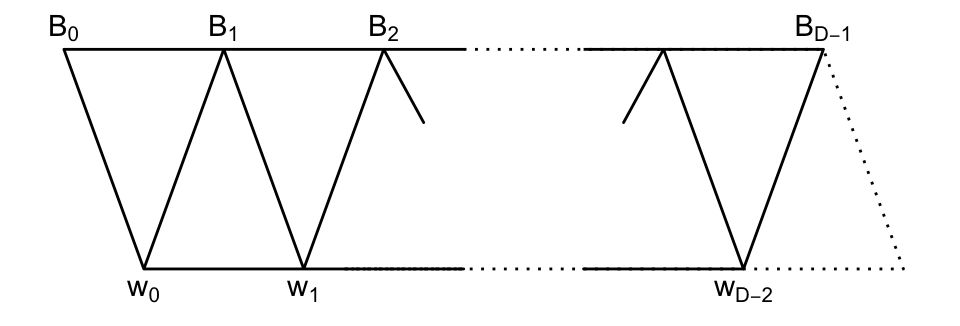
\includegraphics{t-algebra_files/figure-latex/unnamed-chunk-8-1} \end{center}

Vertical lines indicate possible non-orthogonality.

Compute
\begin{equation}
\langle Aw_i, B_j\rangle = \langle w_i, AB_j\rangle, \quad (0\leq i\leq D, \; 0\leq j\leq D-1).\label{eq:wibj}
\end{equation}
\begin{align}
\text{LHS} & = \langle w_{i+1},B_j\rangle + a_i(W)\langle w_i,B_j\rangle + x_i(W)\langle w_{i-1},B_j\rangle\\
\text{RHD}& = b_j\langle w_i, B_{j-1}\rangle + (a_j-c_{j+1}+c_j)\langle w_i, B_j\rangle + c_{j+1}\langle w_i, B_{j+1}\rangle.
\end{align}
Evaluate for \(i = j-2, j-1, j, j+1\).

Set \(i = j-2\).

\begin{center}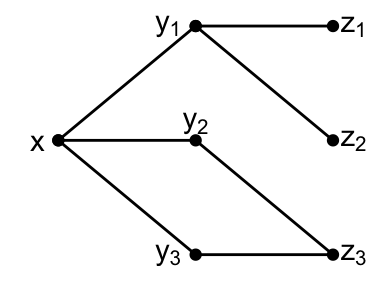
\includegraphics{t-algebra_files/figure-latex/unnamed-chunk-9-1} \end{center}

Then \eqref{eq:wibj} becomes
\[\langle w_{j-1}, B_j\rangle = b_j\langle w_{j-2},B_{j-1}\rangle \quad (2\leq j\leq D-1).\]
By induction,
\[\langle w_{j-1}, B_j\rangle = b_2b_3\cdots b_j\langle w_{0},B_{1}\rangle \quad (1\leq j\leq D-1).\]
Define
\[\gamma_0 = \frac{\langle w_0, B_1\rangle}{\langle w_0, B_0\rangle}.\]
(We will show \(\gamma_0 = 1+a_0(W)\).)

Then,
\begin{equation}
\langle w_{j-1},B_j\rangle = b_2b_3\cdots b_j\gamma_0\langle w_0, B_0\rangle. \label{eq:wj-1bj}
\end{equation}

Set \(i = j+1\).
Then \eqref{eq:wibj} becomes
\[x_{j+1}(W)\langle w_j, B_j\rangle = c_{j+1}\langle w_0, B_{j+1}\rangle \quad (0\leq j\leq d).\]
Hence,
\begin{equation}
\langle w_j, B_j\rangle = \frac{x_1(W)\cdots w_j(W)}{c_1c_2\cdots c_j}\langle w_0, B_0\rangle \quad (0\leq j\leq d). \label{eq:wjbj}
\end{equation}

Set \(i = j-1\).
Then \eqref{eq:wibj} becomes
\[
\langle w_j, B_j\rangle + a_{j-1}(W)\langle w_{j-1}, B_j\rangle
 = (a_j-c_{j+1}+c_j)\langle w_{j-1},B_j\rangle + b_j\langle w_{j-1},B_{j-1}\rangle.
\]
Evaluate this using \eqref{eq:wj-1bj} and \eqref{eq:wjbj}. \((\langle w_0, B_0\rangle \neq 0)\). Then we have
\[\frac{w_1(W)\cdots x_j(W)}{c_1\cdots c_j}+(a_{j-1}(W)-a_j+c_{j+1}-c_j)b_2\cdots b_j\gamma_0 = b_j\frac{x_1(W)\cdots x_{j-1}(W)}{c_1\cdots c_{j-1}},\]
\[\left(\gamma_i:=\frac{c_2c_3\cdots c_{i+1}b_2b_3\cdots b_{i+1}\gamma_0}{x_1(W)x_2(W)\cdots x_i(W)} \right).\]
\[\frac{x_j(W)}{c_j}  = b_j + \frac{c_1c_3\cdots c_{j-1}b_2b_3\cdots b_{j}\gamma_0}{x_1(W)x_2(W)\cdots x_{j-1}(W)}(a_j+c_j-c_{j+1}-a_{j-1}).\]
So,
\[x_j(W)  = c_jb_j + \gamma_{j-1}(a_j+c_j-c_{j+1}-a_{j-1}(W)).\]
This proves \eqref{eq:xi}.

Set \(i = j\).
Then \eqref{eq:wibj} becomes
\[
a_j(W)\langle w_j, B_j\rangle + x_{j}(W)\langle w_{j-1}, B_j\rangle
 = (a_j-c_{j+1}+c_j)\langle w_{j},B_j\rangle + c_{j+1}\langle w_{j},B_{j+1}\rangle.
\]
\[
(a_j(W) - (a_j-c_{j+1}+c_j))\frac{x_1(W)\cdots x_j(W)}{c_1\cdots c_j}
x_j(W)b_2\cdots b_j\gamma_0 - c_{j+1}b_2\cdots b_{j+1}\gamma_0 = 0.
\]
Thus,
\[a_j(W)-(a_j-c_{j+1}+c_{j}) + \frac{c_1\cdots c_jb_2\cdots b_j\gamma_0}{x_1(W)\cdots x_{j-1}(W)} - \frac{c_1\cdots c_jc_{j+1}b_2\cdots b_{j+1}\gamma_0}{x_1(W)\cdots x_j(W)} = 0,\]
or
\[a_j(W) = a_j + c_j - c_{j+1} - \gamma_{j-1} + \gamma_j.\]
This proves \eqref{eq:ai}.

Also by setting \(i = j = 0\), we have
\begin{align}
a_0(W)\langle w_0, B_0\rangle & = (a_0-c_1+c_0)\langle w_0, B_0\rangle + c_1\langle w_0, B_1\rangle\\
& = -\langle w_0, B_0\rangle + \gamma_0\langle w_0, B_0\rangle.
\end{align}
Hence,
\[\gamma_0 = 1 + a_0(W).\]
Both \(a_i(W)\) and \(x_i(W)\) are algebraic integers, since they are eigenvalues of matrices with integer entries, namely,
\[E^*_{i+1}(x)AE^*_{i+1}(x) \; \text{ and }\; E^*_i(x)AE^*_{i+1}(x)AE^*_i(x).\]

Also \(\gamma_0 = 1+a_0(W)\) is an algebraic integer, and \(\gamma_i - \gamma_{i-1}\) is an algebraic integer by \eqref{eq:xi}.

Hence, \(\gamma_i\) is an algebraic integer by induction.

This completes the proof of Theorem \ref{thm:endpoint1}.
\end{proof}

\begin{example}[D=2]
\[D = 2 \Leftrightarrow \text{strongly regular}.\]
Free parameters are \(k, a_1, c_2\).
Let \(W\) be an irreducible module of endpoint \(1\).
The matrix representation of \(A|_W\) is
\[\begin{pmatrix}
a_0(W) & x_1(W)\\ 1 & a_1(W)
\end{pmatrix}.\]
\(a_0(W)\): free.
\begin{align}
x_1(W) & = c_1b_1 + (a_0(W) + 1)(a_1 + c_1 - c_2 - a_0(W))\\
& = k - a_1 - 1 + a_1a_0(W) + a_0(W) - c_2a_0(W) - a_0(W)^2\\
& \qquad + a_1 + a - c_2 - a_0(W)\\
& = a_1a_0(W) - c_2a_0(W) + k - c_2 - a_0(W)^2,\\
\gamma_1 & = 0,\\
a_1(W) & = -(a_0(W)+1) + a_1 + c_1 - c_2\\
& = -a_0(W) + a_1 - c_2.
\end{align}

Then the matrix has eigenvalues \(\theta, \theta_1\).
There is one feasible condition: \(a_0(W)\) is an algebraic integer.
\end{example}

\begin{example}[D=3]
Free parameters \(c_2, c_3, k, a_1, a_2\). The matrix representation becomes
\[
A|_{W} = \begin{pmatrix} a_0(W) & x_1(W) & 0 \\ 1 & a_1(W) & x_2(W)\\ 0 & 1 & a_2(W) \end{pmatrix}.\]
Here, \(a_0(W)\) is free \((=\gamma - 1)\)
\begin{align}
x_1(W) & = k - 1 - a_1 + \gamma_0(a_1 + 1 - c_2 - a_0(W))\\
& = \gamma_0(a_1 - c_2 - a_0(W)) + k - a_1 + a_0(W).
\end{align}
Set
\[\gamma_1(W) = \frac{c_2b_2\gamma_0}{x_1(W)}.\]
\begin{align}
a_1(W) & = \gamma_1 - \gamma_0 + a_1 + 1 - c_2\\
x_2(W) & = \gamma_1(a_2 - c_3 - a_1(W)) + c_2(\gamma_0 + b_1 - a_2 + a_1(W))\\
a_2(W) & = -\gamma_1 + a_2 + c_2 - c_2.
\end{align}
The matrix has eigenvalues, \(\theta, \theta_2, \theta_3\).

There are two feasibility conditions; \(\gamma_0, \gamma_1\) are algebraic integers.

For arbitrary \(D\), there are \(D-1\) feasibility conditions;
\(\gamma_0, \gamma_1, \ldots, \gamma_{D-1}\) are algebraic integers.
\end{example}

\begin{lemma}
\protect\hypertarget{lem:aixigi}{}\label{lem:aixigi}With the notation of Theorem \ref{thm:endpoint1}, suppose
\[f_W = \frac{k-\lambda}{k} \quad (\text{so, }\; a_0(W) = -1).\]
Then,
\begin{align}
a_i(W) & = a_i + c_i - c_{i+1} \quad (0\leq i\leq D-1)\\
x_i(W) & = b_ic_i \quad (1\leq i\leq D-1)\\
\gamma_i(W) & = 0 \quad (0\leq i\leq D-1).
\end{align}
\end{lemma}

\begin{proof}
Since \(\gamma_0 = a_0(W) + 1\), \(\gamma_i = 0\).
\end{proof}

\hypertarget{lec17}{%
\chapter{Association Schemes}\label{lec17}}

\textbf{Monday, March 1, 1993}

\textbf{Review}

Let \(\Gamma = (X, E)\) be a distance-regular graph of diameter \(D\geq 2\). Pick a vertex \(x\in X\).

Let \(W\) be a thin irreducible \(T(x)\)-module with endpoint \(r = 1\), diameter \(d = D-1\) or \(D-2\), and \(r_0 = a_0(W) + 1\).

Show
\[\gamma_i = \frac{c_2c_2\cdots c_{i+1}b_2b_3\cdots b_{i+1}\gamma_0}{x_1(W)\cdots x_i(W)},\]
\(a_i(W)\) and \(x_i(W)\) are all algebraic integers in \(\mathbb{Q}[\gamma_0]\), where
\begin{align}
x_i(W) & = c_ib_i + \gamma_{i-1}(a_i + c_i - c_{i+1}-a_{i-1}(W)) && (1\leq i\leq d)\\
a_i(W) & = \gamma_i - \gamma_{i-1} + a_i + c_i - c_{i+1} && (1\leq i\leq d)
\end{align}

Certainly, \(x_i(W)\), \(\gamma_i\), and \(a_i(W)\) are in \(\mathbb{Q}[\gamma_0]\) by the above lines and so on.
\[\gamma_0 \to a_0(W) \to x_1(W) \to \gamma_1 \to a_1(W)\to x_1(W) \to \cdots .\]
Recall some \(B\in \mathrm{Mat}_n(\mathbb{C})\) is integral whenever
\[B\in \mathrm{Mat}_n(\mathbb{Z}).\]
In this case, the characteristic polynomial
\[\det(\lambda I - B) = \lambda^n + \alpha_{n-1}\lambda^{n-1} + \cdots + \alpha_0, \; \text{ for some }\; \alpha_0, \ldots, \alpha_{n-1}\in \mathbb{Z}.\]
Hence, eigenvalues of \(B\) are algebraic integers.
But \(a_i(W)\) is an eigenvalue of an integral matrices,
\[B = E^*_{i+1}(x)AE^*_{i+1}(x).\]
Hence, \(a_i(W)\) is an algebraic integer.

Also, \(x_i(W)\) is an eigenvalue of an integral matrix
\[B = E^*_i(x)AE^*_{i+1}(x)AE^*_i(x).\]
So \(x_i(W)\) is an algebraic integer.
\[\gamma_i - \gamma_{i-1} = a_i(W) - a_i - c_i + c_{i+1}\]
is an algebraic integer.

Since \(\gamma_0 = a_0(W) + 1\) is an algebraic integer, we find \(\gamma_i\) is an algebraic integer for all \(i\).

\begin{definition}
\protect\hypertarget{def:association-scheme}{}\label{def:association-scheme}A (commutative) association scheme\index{association scheme} is a configuration \(Y = (X, \{R_i\}_{0\leq i\leq D})\), where \(X\) is a finite nonempty set (of vertices),
\(R_0, R_1, \ldots, R_D\) are nonempty subsets of \(X\times X\) such that

\((i)\) \(R_0 = \{(x,x)\mid x\in X\}\),

\((ii)\) \(R_0 \cup \cdots \cup R_D = X\times X \quad (\text{disjoint union})\),

\((iii)\) for every \(i\), \(R_i^\top = \{(y,x)\mid xy\in R\} = R_{i'}\) for some \(i'\in \{0,1,\ldots, D\}\),

\((iv)\) for every \(h, i, j\) (\(0\leq h, i, j\leq D\)), and every \(x,y\in X\) such that \((x,y)\in R_h\),

\[p^h_{ij} = |\{z\in X\mid (x,z)\in R_i, \; (z,y)\in R_j\}|\]
depends only on \(h, i, j\) and not on \(x,y\); and

\((v)\) \(p^h_{ij} = p^h_{ji}\) for all \(h,i, j\).

If \(i' = i\) for all \(i\), we say \(Y\) is symmetric\index{symmetrix}.
We call \(D\) the class of scheme and \(R_i\), the \(i\)th relation of \(Y\). We say vertices \(x,y\in X\) are \(i\)-related, or `at distance \(i\)', whenever \((x,y)\in R_i\).

We always assume that a `scheme' is a commutative association scheme.
\end{definition}

Let \(Y = (X, \{R_i\}_{0\leq i\leq D})\) be an association scheme.

\begin{definition}
\protect\hypertarget{def:incidencemat-of-as}{}\label{def:incidencemat-of-as}

The \(i\)-the association matrix\index{association matrix} \(A_i\in \mathbb{Mat}_X(\mathbb{C})\)
\begin{align}
(A_i)_{xy} & = \begin{cases} 1 & \text{if}\; (x,y)\in R_i\\
0 & \text{if}\; (x,y)\not\in R_i,\end{cases} && (x,y\in X, 0\leq i\leq D)
\end{align}
Then,

\((i')\) \(A_0 = I\).

\((ii')\) \(A_0 + A_1 + \cdots + A_D = J\) (= all 1's matrix).

\((iii')\) \(A_i^\top = A_{i'}\) (\(0\leq i\leq D\)).

\((iv')\) \({\displaystyle A_iA_j = \sum_{h=0}^D p^h_{ij}A_h\quad }\) \((0\leq i,j\leq D)\).

\((v')\) \(A_iA_j = A_jA_i\).

\(M := \mathrm{Span}_{\mathbb{C}}(A_0, \ldots, A_D)\) (Bose-Mesner algebra of \(Y\)) is a commutative \(\mathbb{C}\)-algebra of dimension \(D+1\).

\end{definition}

Observe:
\[Y \text{ is symmetric} \leftrightarrow A_i^\top = A_i \text{ for all } i \leftrightarrow M \text{ is symmetric}.\]

\begin{example}
\protect\hypertarget{exm:dr}{}\label{exm:dr}Let \(\Gamma = (X, E)\) be distance-regular of diameter \(D\). Set
\begin{align}
R_i & = \{(x,y)\mid \partial(x,y) = i\} && (0\leq i\leq D).
\end{align}
Then,
\[Y = (X, \{R_i\}_{0\leq i\leq D})\]
is a symmetric scheme.
\[i\text{-th association matrix} = i\text{-th distance matrix} \quad \text{for all $i$.}\]
\end{example}

\begin{example}
\protect\hypertarget{exm:gen-tr}{}\label{exm:gen-tr}Suppose a group \(G\) acts transitively on a seet \(X\). Assume \(G\) is generously transitive, i.e.,
\[\text{for all }x,y\in X, \text{ there exists }g\in G \text{ such that }gx = y, gy = x.\]
Then \(G\) acts on \(X\times X\) by rule;
\[g(x,y) = (gx, gy), \quad \text{for all }\; g\in G, \text{ and for all }x,y\in X.\]
Let \(R_0, \ldots, R_D\) denote orbits of \(G\) on \(X\times X\).

Observe that \(R_i^\top = R_i\) for all \(i\) by generously transitivity, and
\[Y = (X, \{R_i\}_{0\leq i\leq D})\]
is a symmetric scheme.
\end{example}

\begin{exercise}
\protect\hypertarget{exr:gen-tr-case}{}\label{exr:gen-tr-case}In Example Example \ref{exm:gen-tr}, Bose-Mesner algebra
\begin{align}
M & = \{B\in \mathrm{Mat}_X(\mathbb{C}) \mid Bg = gB, \text{ for all }g\in G\}\\
& = \text{the commuting algebra of $G$ on $X$.}
\end{align}
Here, we view each \(g\in G\) as a permutation matrix in \(\mathrm{Mat}_X(\mathbb{C})\) satisfying
\[g\hat{x} = \widehat{gx} \quad \text{for all }x\in G.\]
\end{exercise}

\begin{example}
\protect\hypertarget{exm:centralizer-alg}{}\label{exm:centralizer-alg}Let \(G\) be any finite group. \(G\) acts on \(X = G\) by conjugation.
\[G\times X \to X, \quad (g,x)\mapsto gxg^{-1}.\]
Let \(C_0, C_1, \ldots, C_D\) denote orbits (i.e., conjugacy classes), and let \(C_0 = \{1_G\}\).
Claim that \(Y = (X, \{R_i\}_{0\leq i\leq D})\) is a commutative scheme (not symmetric in general).

\((i)\) \(R_0 = \{xx\mid x\in X\}\) as \(C_0 = \{1_G\}\).

\((ii)\) \(R_0, \ldots, R_D\) is a partition of \(X\times X\) since \(C_0, \ldots, C_D\) is a partition of \(X = G\).

\((iii)\) \(R_i^\top = R_{i'}\), where \(C_{i'} = \{g^{-1}\mid g\in C_i\}\).

\((iv)\) Set \(H = G\oplus G\), the direct sum. Then \(H\) acts on \(X = G\):

\[\text{for all }h = (g,gz), \text{for all }x\in X, \quad h(x) = gx(gx)^{-1} = gxz^{-1}g^{-1}.\]
\[R_i = \{(x,y)\mid x^{-1}y\in C_i\}, \; h_i\in C_i, \; x^{-1}y = gh_ig^{-1}.\]
\begin{align}
(x,y) & = (x, xgh_ig^{-1})\\
& = (xgg^{-1}, xgh_ig^{-1})\\
& = (xg, g)(1,h_i).
\end{align}
So, \(R_0, \ldots, R_D\) are the orbits of \(H\) on \(X\times X\).

\((v)\) \(p^h_{ij} = p^h_{ji}\)?

Fix \(i,j, h\) and \(x, y\in X\) with \((x,y)\in R_h\). Set
\begin{align}
S & = \{z\in X\mid (x,z)\in R_i, \; (z,y)\in R_j\}\\
T & = \{z\in X\mid (x,z)\in R_j, \; (z,y)\in R_i\}.
\end{align}
Show \(|S| = |T|\).
\[\text{For all }z\in S, \text{ set } \hat{z} = xz^{-1}y.\]
Observe, \(\hat{z}\in T\).
\begin{align}
x^{-1}z\in C_i \quad  & x^{-1}\hat{z} = x^{-1}xz^{-1}y\in C_j\\
z^{-1}y\in C_j \quad  & \hat{z}^{-1}y = y^{-1}zx^{-1}x^{-1}y = y^{-1}x(x^{-1}z)x^{-1}y \in C_i.
\end{align}
Observe
\[S\to T \quad (z\mapsto z^{-1}) \quad \text{is one-to-one and onto.}\]
\end{example}

\hypertarget{lec18}{%
\chapter{Polynomial Schemes}\label{lec18}}

\textbf{Wednesday, March 3, 1993}

\begin{lemma}
\protect\hypertarget{lem:dr-scheme}{}\label{lem:dr-scheme}Let \(Y = (X, \{R_i\}_{0\leq i\leq D})\) denote the symmetric scheme with associated matrices \(A_0, A_1, \ldots, A_D\). Then the following are equivalent.

\((i)\) The graph \(\Gamma = (X, R_1)\) is distance-regular, and \(R_0, \ldots, R_D\) are labelled so that

\[R_i = \{xy\mid \partial(x,y) = i\}.\]

\((ii)\) There exists \(f_i\in \mathbb{C}[\lambda]\), \(\deg f_i = i\) such that \(f_i(A_1) = A_i\) for all \(i\) with \(0\leq i\leq D\).

\((iii)\) The parameter \(p^h_{ij}\)

\[\begin{cases} = 0 & \text{if one of $h, i, j$ is larger than the sum of the other two,}\\
\neq 0 & \text{if one of $h,i,j$ is equal to the sum of the other two.}\end{cases}\]
\end{lemma}

\begin{proof}
\leavevmode

\((i)\Rightarrow (ii)\): Lemma \ref{lem:incidence-matrices}.

\((ii)\Rightarrow (iii)\): Define

\[k_i \equiv p^0_{ii} = |\{z\mid z\in X, \; \partial(x,z) = i, \; ((x,z)\in R_i)\}|\]
for any \(x\in X\).
Then \(k_i \neq 0\) \((0\leq i\leq D)\), \(k_0 = 1\).

(By symmetricity, \((x,y)\in R_i\) if and only if \((y,x)\in R_i\).)

Claim.
\begin{align}
k_hp^h_{ij} & = k_ip^i_{hj} = k_jp^j_{ih}\\
& = |X|^{-1}|\{xyz\in X^3\mid \partial(x,y) = h, \partial(x,z) = i, \partial(y,z) = j\}|.
\end{align}
\emph{Pf.}
The number of \(xyz\in X^3\), \(\partial(x,y) = h, \partial(x,z) = i, \partial(y,z) = j\) is equal to
\[|X|k_hp^h_{ij} = |X|k_ip^i_{hj} = k_jp^j_{ih}.\]

In particular,
\[p^h_{ij} = 0 \leftrightarrow p^i_{hj} =0 \leftrightarrow p^j_{ih} = 0.\]
Hence, it suffices to show
\[\begin{cases}
p^h_{ij} = 0 & \text{if }\; h > i+j\\
p^h_{ij} \neq 0 & \text{if }\; h = i+j.
\end{cases}\]

Fix \(i,j\). Without loss of generality, we may assume that \(i+j\leq D\) as trivial otherwise.
\[f_i(A)f_j(A) = A_iA_j = \sum_{\ell = 0}^Dp^{\ell}_{ij}A_\ell = \sum_{\ell=0}^Dp^\ell_{ij}f_\ell(A).\]
\begin{align}
i + j & = \deg \mathrm{LHS}\\
& = \deg \mathrm{RHS}\\
& = \max\{\ell\mid p^\ell_{ij}\neq 0\}.
\end{align}

\((iii)\Rightarrow (i)\)

Let \(A = A_1\), and consider a graph \(\Gamma\) with adjacency matrix \(A\).
\begin{align}
AA_j & = \sum_{h}p^h_{1j}A_h\\
& = p^{j+1}_{1j} A_{j+1} + p^j_{1j}A_j + p^{j-1}_{1j}A_{j-1}.
\end{align}

Then, \(p^{j+1}_{1j} \neq 0 \neq p^{j-1}_{1j}\).

Fix a vertex \(x\in X\), and set \(R_i(x) = \{y\mid (x,y)\in R_i\}\).

Then each \(y\in R_i(x)\) is adjacent in \(\Gamma\) to exactly
\begin{align}
p^i_{1,i+1} & \neq 0  \quad \text{vertices in }\; R_{i+1}(x),\\
p^i_{1i} & \qquad \text{vertices in }\; R_{i}(x),\\
p^i_{1,i-1} & \neq 0 \quad \text{vertices in }\; R_{i-1}(x).
\end{align}
Hence, by induction,
\begin{align}
R_i(x) & = \{y\mid \partial(x,y) = i \text{ in }\Gamma\} && (0\leq i\leq D),
\end{align}
and \(\Gamma\) is distance regular.

\end{proof}

\hypertarget{lec19}{%
\chapter{Commutative Association Schemes}\label{lec19}}

\textbf{Friday, March 5, 1993}

\begin{lemma}
\protect\hypertarget{lem:ei}{}\label{lem:ei}

Let \(Y = (X, \{R_i\}_{0\leq i\leq D})\) be a commutative scheme with Bose-Mesner algebra \(M\).

Then there exists a basis \(E_0, E_1, \ldots, E_D\) for \(M\) such that

\((i)\) \(E_0 = |X|^{-1}J\).

\((ii)\) \(E_iE_j = E_jE_i = \delta_{ij}E_i\) \(\quad (0\leq i,j\leq D)\).

\((iii)\) \(E_0 + E_1 + \cdots + E_D = I\).

\((iv)\) \(E_i^\top = \overline{E_i} = E_{\hat{i}}\) for some \(\hat{i}\in \{0, 1, \ldots, D\}\).

\end{lemma}

\begin{proof}
\(M\) acts on Hermitean space \(V = \mathbb{C}^n\) \((n = |X|)\).

If \(W\) is an \(M\)-module, so is \(W^\bot\).

Each irreducible \(M\)-module is \(1\) dimensional by commutativity of \(M\). So \(V\) is orthognal direct sum of \(1\)-dimensional \(M\)-modules.

Let \(v_1, \ldots, v_n\) be an orthonormal basis for \(V\) consisiting of eigenvectors for all \(m\in M\).

Set \(P\in \mathrm{Mat}_X(\mathbb{C})\) so that the \(i\)-th column of \(P\) is equal to \(v_i\). So,
\[\bar{P}^\top P = I = P\bar{P}^\top = \bar{P}P^\top,\]
and \(P\) is unitary.

Also, for all \(m\in M\),
\begin{align}
P^{-1}mP & = \text{diagonal}\\
& = \mathrm{diag}(\theta_1(m), \ldots, \theta_n(m)).
\end{align}
for some functions
\[\theta_i: M \longrightarrow \mathbb{C}.\]
Observe: each \(\theta = \theta_i\) is a character of \(M\), i.e.,
\[\theta: M\longrightarrow \mathbb{C}\]
is a \(\mathbb{C}\)-algebra homomorphism.

Observe: the \(\theta_1, \ldots, \theta_n\) are not all distinct.

Let \(\sigma_0, \ldots, \sigma_r\) denote distinct elements of
\[\theta_1, \ldots, \theta_n.\]
Say \(\sigma_i\) appears \(m_i\) times.
Without loss of generality, we may assume that
\[P^{-1}mP = \begin{pmatrix}\sigma_0(m)I_{m_0} & O & O &  O \\
O & \sigma_1(m)I_{m_1} & O &  O\\
O & O & \ddots & O \\
O & O & O & \sigma_r(m)I_{m_r}
\end{pmatrix}.\]
Set
\[E_i = P\begin{pmatrix} O & O & O\\
O & I_{m_i} & O\\
O & O & O \end{pmatrix}P^{-1},\]
where \(I_{m_i}\) is in the \(i\)-th block.

Then,
\[E_iE_j = \delta_{ij}E_i \quad (0\leq i,j\leq r),\]
\[E_0 + E_1 + \cdots + E_r = I.\]
Hence for all \(m\in M\),
\[m = \sum_{i=0}^r \sigma_i(m)E_i \in \mathrm{Span}(E_0, \ldots, E_r).\]
So,
\[M \subseteq \mathrm{Span}(E_0, \ldots, E_r).\]
Since \(E_0,\ldots, E_r\) are linearly independent, \(r\geq D\).

Show \(E_i\in M\).

Claim 1. For all distinct \(i, j\) \(\quad (0\leq i, j\leq D)\), there exists \(m\in M\) such that \(\sigma_i(m)\neq 0\), \(\sigma_j(m)=0\).

\emph{Pf of Claim 1.}
\(\sigma_i\neq \sigma_j\) implies that there exists \(m'\in M\) such that \(\sigma_i(m')\neq \sigma_j(m')\).

Set \(m = m'-\sigma_j(m')I\). Then,
\begin{align}
\sigma_j(m) & = \sigma_j(m') - \sigma_j(m')  = 0,\\
\sigma_i(m) & = \sigma_i(m') - \sigma_j(m')  \neq 0.
\end{align}

Claim 2. \(E_i\in M\) \(\quad (0\leq i \leq D)\).

\emph{Pf of Claim 2.}
Fix a vertex \(x\in X\). For all \(j\neq i\), there exists \(m_j\in M\) such that
\[\sigma_i(m_j)\neq 0, \quad \sigma_j(m_j) = 0, \quad i\neq j.\]
Observe
\[s = \sigma_i\left(\prod_{\ell\neq i}m_\ell\right) \neq 0.\]
Set
\[m^* = \left(\prod_{\ell\neq i}m_\ell\right) s^{-1}.\]
Observe
\[\sigma_i(m^*) =1, \quad \sigma_j(m^*) = 0, \quad \text{for all }j\neq i \quad (0\leq j\leq D).\]
So
\[P^{-1}m^*P = \begin{pmatrix} O & O & O\\
O & I_{m_i} & O\\
O & O & O \end{pmatrix}.\]
We have
\[E_i = m^*\in M.\]
Now \(r = D\), \(M = \mathrm{Span}(E_0, \ldots, E_D)\) and \(E_0, \ldots, E_D\) is a basis for \(M\).

Observe
\[P^{-1}E_iP = \begin{pmatrix} O & O & O\\
O & I_{m_i} & O\\
O & O & O \end{pmatrix}\]
implies
\[P^{-1}\overline{E_i}^\top P = \bar{P}^\top \overline{E_i}^\top \overline{P^{-1}}^\top = \begin{pmatrix} O & O & O\\
O & I_{m_i} & O\\
O & O & O \end{pmatrix}^\top = P^{-1}E_i P.\]
Hence,
\[\overline{E_i}^\top = E_i.\]
\(E_0^\top, \ldots, E_D^\top\) are nonzero matrices satisfying
\[E_i^\top E_j^\top = \delta_{ij}E_i^\top,\]
\[E_0^\top + E_1^\top + \cdots + E_D^\top = I.\]
Each \(E_i^\top\) is a linear combination of \(E_0, \ldots, E_D\) with coefficientss that are \(0\) or \(1\), and for no two \(E_i\)'s are coefficients of any \(E_j\) both \(1\)'s.

So, \(E_0^\top, \ldots, E_D^\top\) is a permutation of \(E_0, \ldots, E_D\).

Observe \(J = A_0 + \cdots + A_D\in M\).

The matrix \(|X|^{-1}J\) is an idempotent of rank \(1\).

So, without loss of generality we may assume that
\[E_0 = \frac{1}{|X|}J.\]
We have the assertions.
\end{proof}

Define entry-wise product \(\circ\) on \(\mathrm{Mat}_X(\mathbb{C})\).
\[A_i \circ A_j = \delta_{ij}A_i.\]
So, \(M\) is closed under \(\circ\).
\[E_i \circ E_j = \frac{1}{|X|}\sum_{h=0}^D q^h_{ij}E_h.\]
The numbers \(q^h_{ij}\) is called Krein parameters of \(Y\).

Claim. \(q^h_{ij}\in \mathbb{R}\).

\emph{Pf.}
\begin{align}
\frac{1}{|X|}\sum_{h=0}^D \overline{q^h_{ij}}E_h & = \frac{1}{|X|}\sum_{h=0}^D \overline{q^h_{ij}}\overline{E_h}^\top \\
& = (\overline{E_i\circ E_j})^\top \\
& = E_i\circ E_j \\
& = \frac{1}{|X|}\sum_{h=0}^D q^h_{ij}E_h.
\end{align}
Hence, \(q^h_{ij} = \overline{q^h_{ij}}\).

Observe
\(A_0, \ldots, A_D\), \(E_0, \ldots, E_D\) are bases for \(M\). Hence, there exist \(p_i(j)\), \(q_i(j)\in \mathbb{C}\) such that
\begin{align}
A_i & = \sum_{j = 0}^D p_i(j)E_j\\
E_i & = \frac{1}{|X|}\sum_{j=0}^D q_i(j)A_j.
\end{align}
Taking transpose and conjugate we find,
\begin{align}
\overline{p_i(j)} & =  p_i(j)  =  p_{i'}(\hat{j}) && (0\leq i,j\leq D)\\
\overline{q_i(j)} & =  q_i(j)  =  q_{\hat{i}}({j}') && (0\leq i,j\leq D).
\end{align}

Fix a vertex \(x\in X\). Define
\[E^*_i \equiv E^*_i(x) \in \mathrm{Mat}_X(\mathbb{C})\]
to be a diagonal matrix such that
\[(E^*_i)_{xy} = \begin{cases} 1 & \text{if } (x,y)\in R_i\\ 0 & \text{if } (x,y)\not\in R_i
\end{cases} \quad (0\leq i\leq D, y\in X.)\]
Then,
\[E^*_iE^*_j = \delta_{ij}E^*_i,\]
\[E^*_0 + \cdots + E^*_D = I,\]
\[(E^*_i)^\top = \overline{E^*_i} = E^*_i.\]

\begin{definition}
\protect\hypertarget{def:dual-bose-mesner}{}\label{def:dual-bose-mesner}Dual Bose-Mesner algebra \index{dual Bose-Mesner algebra}: \(M^* \equiv M^*(x)\) with respect to \(x\) is
\[\mathrm{Span}(E^*_0, \ldots, E^*_D).\]
\end{definition}

Define dual associate matrices\index{dual associate matrix} \(A_0^*, \ldots, A^*_D\).
Indeed \(A^*_i \equiv A^*_i(x)\in \mathrm{Mat}_X(\mathbb{C})\) is a diagonal matrix with
\[(A_i^*)_{yy} = |X|(E_i)_{xy}\quad (y\in X).\]
\(A^*_i\) is a diagonal matrix having the row \(x\) of \(E_i^*\) on the diagonal.

Observe
\begin{align}
A^*_i & = \sum_{j=0}^Dq_i(j)E^*_j \quad \left(E_i = \frac{1}{|X|}\sum_{j=0}^D q_i(j)A_j\right)\\
E^*_i & = \frac{1}{|X|}\sum_{j=0}^D p_i(j)A^*_j \quad \left(A_i = \sum_{j=0}^D p_i(j)E_j\right).
\end{align}
So, \(A^*_0, \ldots, A^*_D\) form a basis for \(M^*\).

Also,
\[A^*_iE^*_j = q_i(j)E^*_j.\]
\[\left(A^*_iE^*_j = \sum_{h=0}^D q_i(h)E^*_hE^*_j = q_i(j)E^*_j.\right)\]
So, \(q_i(j)\) are dual eigenvalues of \(A^*_i\).

Observe,
\[A^*_0 = I, \quad A^*_0 + \cdots + A^*_D = |X|E^*_0, \quad \overline{A^*_i} = A^*_{\hat{i}},\]
\[A^*_iA^*_j = \sum_{h=0}^D q^h_{ij}A^*_h \quad (0\leq i,j\leq D).\]

\textbf{HS MEMO}

\emph{Proof.}
\[(A^*_0)_{yy} = |X|(E_0)_{xy} = (J)_{xy} = 1.\]
\[A^*_0 + \cdots + A^*_D = \sum_{i=0}^D\sum_{j=0}^D q_i(j)E^*_j = |X|E^*_0.\]
Note that
\[I = E_0 + \cdots + E_D = \frac{1}{|X|}\sum_{i=0}^D\sum_{j=0}^D q_i(j)A_j.\]
\[\sum_{i=0}^D q_i(j) = \delta_{j0}|X|.\]
\[\overline{A^*_i} = \sum_{j=0}^D\overline{q_i(j)}E^*_j = \sum_{j=0}^D q_{\hat{i}}(j)E^*_j = A^*_{\hat{i}}.\]
\begin{align}
(A^*_iA^*_j)_{yy} & = |X|^2 (E_i)_{xy}(E_j)_{xy}\\
& = |X|^2(E_i\circ E_j)_{xy}\\
& = |X|\sum_{h=0}^D q^h_{ij}(E_h)_{xy}\\
& = \sum_{h=0}^D q^h_{ij}(A^*_h)_{yy}.
\end{align}

The following statements will be proved after a couple of lemmas in the next lecture.

\textbf{Lemma.}
Let \(Y = (X, \{R_i\}_{0\leq i\leq D})\) be a commutative scheme. Fix a vertex \(x\in X\), and set \(E^*\equiv E^*_i(x)\) and \(A^*_i \equiv A^*(x)\).
Then the following hold.

\((i)\) \(E^*_iA_jE^*_k = O\) if and only if \(p^k_{ij} = 0\) for \(0\leq i,j,k\leq D\).

\((ii)\) \(E_iA^*_jE_k = O\) if and only if \(q^k_{ij} = 0\) for \(0\leq i,j,k\leq D\).

\hypertarget{lec20}{%
\chapter{Vanishing Conditions}\label{lec20}}

\textbf{Monday, March 15, 1993} (Monday after Spring break)

\begin{lemma}
\protect\hypertarget{lem:pij-qij}{}\label{lem:pij-qij}Let \(Y = (X, \{R_i\}_{0\leq i\leq D})\) be a commutative scheme.

\((i)\) \(p_0(i) = 1\).

\((ii)\) \(p_i(0) = k_i\), where

\[k_i = p^0_{ii'} = |\{y\in X\mid (x,y)\in R_i\}| \quad (x\in X).\]

\((iii)\) \(q_0(i) = 1\).

\((iv)\) \(q_i(0) = m_i\), where

\[m_i = \mathrm{rank} E_i.\]
\end{lemma}

\begin{proof}
\leavevmode

\((i)\) Since \(A_0 = I\) and

\begin{align}
A_0 & = p_0(0)E_0 + p_0(1)E_1 + \cdots + p_0(D)E_D\\
I & = E_0 + E_1 + \cdots + E_D,
\end{align}
\(p_0(i) = 1\) for all \(i\).

\((ii)\) Since

\[A_i = p_i(0)E_0 + p_i(1)E_1 + \cdots + p_i(D)E_D,\]
\(A_i E_0 = p_i(0)E_0\), and
\[k_i J = A_i J = p_i(0)J\]
as there are \(k_i\) \(1\)'s in each row of \(A_i\), we have \(k_i = p_i(0)\).

\((iii)\) Since \(E_0 = |X|^{-1}J\) and

\begin{align}
E_0 & = |X|^{-1}(q_0(0)A_0 + q_0(1)A_1 + \cdots + q_0(D)A_D)\\
|X|^{-1}J & = |X|^{-1}(A_0 + A_1 + \cdots + A_D),
\end{align}
\(q_0(i) = 1\) for all \(i\).

\((iv)\) \(E_i = |X|^{-1}(q_i(0)A_0 + q_i(1)A_1 + \cdots + q_i(D)A_D)\), \(E_i^2 = E_i\), and \(E_i\) is similar to a matrix

\[\begin{pmatrix} I_{m_i} & O \\ O & O\end{pmatrix}.\]
So,
\[m_i = \mathrm{rank}E_i = \mathrm{trace} E_i = \sum_{x\in X}(E_i)_{xx} = |X||X|^{-1}q_i(0) = q_i(0).\]
Note that as
\[E_i = \frac{1}{|X|}\sum_{j=0}^D q_i(j)A_j \to (E_i)_{xx} = \frac{1}{|X|}q_i(0)(A_0)_{xx}.\]
Hence, we have all formulas.

\end{proof}

\begin{lemma}
\protect\hypertarget{lem:phijqhij}{}\label{lem:phijqhij}

With the above notation

\((i)\) \(p^h_{ij} = p^{h'}_{j'i'}\).

\((ii)\) \(k_hp^h_{ij} = k_jp^j_{i'h} = k_ip^i_{hj'}\).

\((iii)\) \(q^h_{ij} = q^{\hat{h}}_{\hat{j}\hat{i}}\).

\((iv)\) \(m_hq^h_{ij} = m_jq^j_{\hat{i}h} = m_iq^i_{h\hat{j}}.\)

\end{lemma}

\begin{proof}
\leavevmode

\((i)\) We have

\begin{align}
\sum_{h = 0}^D p^h_{ij} A_{h'} & = \left(\sum_{h=0}^D p^h_{ij}A_h\right)^\top \\
 & = (A_iA_j)^\top  \\
& = A_j^\top A_i^\top\\
& = A_{j'}A_{i'} \\
& = \sum_{h=0}^D p^{h'}_{j'i'}A_h'.
\end{align}

\((ii)\) Count the following number,

\begin{align} 
& |\{xyz\in X^3 \mid (x,y)\in R_h, (x,z)\in R_i, (z,y)\in R_j\}| \\
& \quad =  |X|k_hp^h_{ij} = |X|k_jp^j_{i'h} = |X|k^i_{hj'}.
\end{align}

\((iii)\)

\begin{align}
\frac{1}{|X|}\sum_{h = 0}^D q^h_{ij} E_{\hat{h}} & = \left(\frac{1}{|X|}\sum_{h=0}^D q^h_{ij}E_h\right)^\top \\
 & = (E_i\circ E_j)^\top  \\
& = E_j^\top \circ E_i^\top\\
& = E_{\hat{j}}E_{\hat{i}} \\
& = \frac{1}{|X|}\sum_{h=0}^D q^{\hat{h}}_{\hat{j}\hat{i}}E_{\hat{h}}.
\end{align}

\((iv)\) Let \(\tau(B)\) denote the sum of the entries in the matrix \(B\).

Observe: \(\tau(B\circ C) = \mathrm{trace}(BC^\top)\).

Observe
\[\tau(E_i\circ E_j \circ E_{\hat{k}}) = \tau((E_i\circ E_j\circ E_{\hat{k}})^\top) = \tau(E_{\hat{i}}\circ E_k \circ E_{\hat{j}}) = \tau(E_k\circ E_{\hat{j}}\circ E_{\hat{i}}).\]
Compute each one.
\begin{align}
\tau(E_i\circ E_j \circ E_{\hat{k}}) & = \mathrm{trace}((E_i\circ E_j)E_k) = \mathrm{trace}\left(\left(\frac{1}{|X|}\sum_{h} q^h_{ij}E_h\right)E_k\right)\\
& = \mathrm{trace}\left(\frac{1}{|X|} q^k_{ij}E_k\right) = \frac{1}{|X|}m_kq^k_{ij},\\
\tau(E_{\hat{i}}\circ E_k \circ E_{\hat{j}}) & = \mathrm{trace}((E_{\hat{i}}\circ E_k)E_{\hat{j}}) = \mathrm{trace}\left(\left(\frac{1}{|X|}\sum_{h} q^h_{\hat{i}k}E_h\right)E_{\hat{j}}\right)\\
& = \mathrm{trace}\left(\frac{1}{|X|} q^j_{\hat{i}k}E_k\right) = \frac{1}{|X|}m_jq^j_{\hat{i}k},\\
\tau(E_k\circ E_{\hat{j}}\circ E_{\hat{i}}) & = \mathrm{trace}((E_k\circ E_{\hat{j}})E_i) = \mathrm{trace}\left(\left(\frac{1}{|X|}\sum_{h} q^h_{k\hat{j}}E_h\right)E_i\right)\\
& = \mathrm{trace}\left(\frac{1}{|X|} q^i_{k\hat{j}}E_i\right) = \frac{1}{|X|}m_iq^i_{k\hat{j}}.
\end{align}
Hence, we have \((iv)\).

\end{proof}

\begin{lemma}
\protect\hypertarget{lem:vanishing-condition}{}\label{lem:vanishing-condition}

Let \(Y = (X, \{R_i\}_{0\leq i\leq D})\) be a commutative scheme. Fix a vertex \(x\in X\), and set \(E^*_i\equiv E^*_i(x)\) and \(A^*_i \equiv A^*(x)\).
Then the following hold.

\((i)\) \(E^*_iA_jE^*_k = O\) if and only if \(p^k_{ij} = 0\) for \(0\leq i,j,k\leq D\).

\((ii)\) \(E_iA^*_jE_k = O\) if and only if \(q^k_{ij} = 0\) for \(0\leq i,j,k\leq D\).

\end{lemma}

\begin{proof}
\leavevmode

\((i)\) Partition rows and columns by \(R_0(x), R_1(x), \ldots, R_D(x)\). Then,

\[E^*_i(x)A_j E^*_h(x)\]
is the \((i,h)\) block of \(A_j\).

Hence this submatrix is zero if and only if there exists no \(y,z\in X\) such that \((x,y)\in R_i\), \((x,z)\in R_h\) and \((y,z)\in R_j\). This is exactly when \(p^h_{ij} = 0\).

\((ii)\) The sum of the squares of norms of entries in \(E_iA^*_jE_k\)

\begin{align}
& = \tau((E_iA^*_jE_k)\circ (\overline{E_jA^*_jE_k}))\\
& = \mathrm{trace}(E_iA^*_jE_k(\overline{E_jA^*_jE_k})^\top)\\
& = \mathrm{trace}(E_iA^*_jE_kA^*_{\hat{j}}E_i)\\
& = \mathrm{trace}(E_iA^*_jE_kA^*_{\hat{j}}) && \text{as $\mathrm{trace}(XY) = \mathrm{trace}(YX)$}\\
& = \sum_{y\in X}(E_iA^*_jE_kA^*_{\hat{j}})_{yy}\\
& = \sum_{y\in X}\left(\sum_{z\in X} (E_i)_{yz}(A^*_j)_{zz}(E_k)_{zy}(A^*_{\hat{j}})_{yy}\right)\\
& = \sum_{y\in X}\left(\sum_{z\in X} (E_{\hat{i}})_{zy}(|X|(E_j)_{xz})(E_k)_{zy}(|X|(E_j)_{yx})\right)\\
& = |X|^2(E_j(E_{\hat{i}}\circ E_k))E_j)_{xx}\\
& = |X|q^j_{\hat{i}k}(E_j)_{xx}\\
& = q^j_{\hat{i}k}m_j \\
& = m_kq^k_{ij}.
\end{align}
Note that since \(|X|E_j = q_j(0)A_0 + q_j(1)A_1 + \cdots q_j(D)A_D\),
\[(E_j)_{xx} = \frac{1}{|X|}q_j(0) = \frac{m_j}{|X|}.\]
Thus, we have \((ii)\).

\end{proof}

\begin{corollary}[Krein Condition]
\protect\hypertarget{cor:qhij}{}\label{cor:qhij}For any commutative scheme \(Y = (X, \{R_i\}_{0\leq i\leq D})\), \(q^h_{ij}\) is a non-negative real number for \(0\leq h, i, j\leq D\).
\end{corollary}

\begin{proof}
Since \(q^h_{ij}m_h\) is a non-negative real by the proof of Lemma \ref{lem:vanishing-condition} \((ii)\).

Note that \(m_h\) is a positive integer.
\end{proof}

An interpretation of the Krein parameters.

Let \(Y = (X, \{R_i\}_{0\leq i\leq D})\) be a commutative scheme with standard module \(V\).

Pick a vector \(v\in V\) with
\[v = \sum_{x\in X}\alpha_x \hat{x}.\]
View \(v\) as a function
\[v: X\longrightarrow \mathbb{C} \quad (x\mapsto \alpha_x).\]
View \(V\) as the set of all functions \(V \longrightarrow \mathbb{C}\). Then the vector space \(V\) together with product of functions is a \(\mathbb{C}\)-algebra.

For
\[v = \sum_{x\in X}\alpha_x \hat{x}, \quad w = \sum_{x\in X}\beta_x \hat{x} \in V,\]
write
\[v\circ w = \sum_{x\in X}\alpha_x\beta_x \hat{x}\]
to represent the product of \(v\) and \(w\) viewed as functions.

\begin{lemma}
\protect\hypertarget{lem:vector-function-product}{}\label{lem:vector-function-product}

With the above notation,

\((i)\) \(A^*_j(x)v = |X|(E_{\hat{j}}\hat{x}\circ v)\) for all \(v\in V\) and for all \(x\in X\).

\((ii)\) \(E_iV\circ E_jV \subseteq \sum_{h: q^h_{ij}\neq 0} E_hV\) for all \(0\leq i, j\leq D\).

\((iii)\) \(E_h(E_i\circ E_jV) = E_hV\) if \(q^h_{ij}\neq 0\) for all \(0\leq h, i, j\leq D\).

\end{lemma}

\hypertarget{lec21}{%
\chapter{Norton Algebras}\label{lec21}}

\textbf{Wednesday, March 17, 1993}

\begin{proof}[Proof of Lemma \ref{lem:vector-function-product}]
\leavevmode

\((i)\) Suppose

\[v = \sum_{x\in X}\alpha_x \hat{x}.\]
Pick a vertex \(z\in X\) and compare \(z\)-coordinate of each side in \((i)\).
\begin{align}
(A^*_j(x)v)_z & = (A^*_j(x))_{zz}v_z = |X|(E_j)_{xz}\alpha_z.\\
|X|(E_{\hat{j}}\hat{x}\circ v)_z & = |X|(E_{\hat{j}}\hat{x})_z\cdot \alpha_z  = |X|(E_j)_{xz}\alpha_z.
\end{align}
Note that \(E_{\hat{j}}\hat{x}\) is the column \(x\) of \(E_{\hat{j}}\), which is the row \(x\) of \(E_j\).

\((ii)\) Fix \(i, j, h\) such that \(q^h_{ij} = 0\).

Claim. \(E_h(E_iV \circ E_jV) = 0\).

\begin{align}
E_h(E_iV \circ E_jV) & = E_h(\mathrm{Span}(v\circ w\mid v\in E_iV, w\in E_jV))\\
& = E_h(\mathrm{Span}(E_i\hat{y}\circ E_j\hat{z}\mid y,z\in X))\\
& = \mathrm{Span}(E_h(E_j\hat{z}\circ E_i\hat{y}\mid y,z\in X)\\
& = \mathrm{Span}((E_hA^*_{\hat{j}}(z)E_i)\hat{y}\mid y,z\in X) && \text{by $(i)$.}
\end{align}
But \(q^h_{ij} = 0\) implies \(q^{\hat{h}}_{\hat{j}\hat{i}} = 0\).

So, by Lemma \ref{lem:vanishing-condition} \((ii)\),
\[ 0 = (E_{\hat{i}}A^*_{\hat{j}}E_{\hat{h}})^\top = E_h A^*_{\hat{j}}E_i.\]
Hence, \(E_h(E_iV\circ E_jV) = 0\).

\((iii)\) Fix \(i, j, h\) such that \(q^h_{ij}\neq 0\). Then,

\[E_h(E_iV \circ E_jV)\subseteq E_hV\]
is clear. We show the other inclusion. Since
\begin{align}
E_i\hat{y} \circ E_j\hat{y} &=  (\text{column $y$ of $E_i$}\circ \text{column $y$ of $E_j$}) \\
&  = \text{column $y$ of $E_i\circ E_j$}\\
&  = (E_i\circ E_j)\hat{y}\\
&  = \left(\frac{1}{|X|}\sum_{h=0}^D q^h_{ij}E_h\right)\hat{y},
\end{align}
we have,
\begin{align}
E_h(E_iV\circ E_jV) & = E_h\mathrm{Span}(E_i\hat{y}\circ E_j\hat{z}\mid y,z\in X)\\
& \supseteq E_h \mathrm{Span}(E_i\hat{y}\circ E_j\hat{y}\mid y\in X)\\
& = \mathrm{Span}(q^h_{ij}E_h\hat{y}\mid y\in X)\\
& = \mathrm{Span}(E_h\hat{y}\mid y\in X) && \text{since $q^h_{ij}\neq 0$}\\
& = E_hV.
\end{align}
This proves the assertion.

\end{proof}

\begin{lemma}
\protect\hypertarget{lem:norton-algebra}{}\label{lem:norton-algebra}

Given a commutative scheme \(Y = (X, \{R_i\}_{0\leq i\leq D})\), fix \(j\) \((0\leq j\leq D)\).
Define a binary multiplication:
\[E_jV \times E_jV \longrightarrow E_jV \quad ((v,w) \mapsto v\ast w = E_j(v\circ w)).\]
Then,

\((i)\) \(v\ast w = w\ast v\), for all \(v,w\in E_jV\),

\((ii)\) \(v\ast (w + w') = v\ast w + v\ast w'\) for all \(v,w,w'\in E_jV\), and

\((iii)\) \((\alpha v)\ast w = \alpha(v\ast w)\) for all \(\alpha \in \mathbb{C}\).

In particular, the vector space \(E_jV\) together with \(\ast\) is a commutative \(\mathbb{C}\)-algebra, (not associative in general).

(\(N_j: (E_jV, \ast)\) is called the Norton algebra \index{Norton algebra} on \(E_jV\).)

\((iv)\) \(v\ast w = 0\) for all \(v, w\in E_jV\) if and only if \(q^j_{jj} = 0\).

\end{lemma}

\begin{proof}
\leavevmode

\((i)-(iii)\) Immediate.

\((iv)\) Immediate from Lemma \ref{lem:vector-function-product} \((ii)\), \((iii)\).

\end{proof}

Let \(Y\), \(j\), \(N_j\) be as in Lemma \ref{lem:norton-algebra}, and \(M\) Bose-Mesner algebra of \(Y\).
Let
\begin{align}
\mathrm{Aut}Y & = \{\sigma\in \mathrm{Mat}_X(\mathbb{C}) \mid \sigma: \text{ permutation matrix }, \sigma \cdot m = m\cdot \sigma \;\text{ for all }m\in M\}\\
& = \{\sigma\in \mathrm{Mat}_X(\mathbb{C}) \mid \sigma: \text{ permutation matrix },\\
& \qquad (x,y)\in R_i \to (\sigma x, \sigma y)\in R_i, \text{ for all } i, \text{ and for all } x,y\in X\}\\
\mathrm{Aut}(N_j) & = \{\sigma: E_jV \to E_jV \mid \sigma \text{ is a  $\mathbb{C}$-algebra isomorphim},i.e.,\\
& \qquad \sigma(v\ast w) = \sigma(v)\ast\sigma(w) \text{ for all }v, w\in E_jV\}.
\end{align}

\begin{lemma}
\protect\hypertarget{lem:autom-of-norton-algebra}{}\label{lem:autom-of-norton-algebra}

Let \(Y, j, \ast\) be as in Lemma \ref{lem:norton-algebra}.

\((i)\) \(E_jV\) is a module for \(\mathrm{Aut}(Y)\).

\((ii)\) \(\sigma|_{E_jV}\in \mathrm{Aut}(N_j)\) for all \(\sigma \in \mathrm{Aut}(Y)\).

\((iii)\) \(\mathrm{Aut}Y \longrightarrow \mathrm{Aut}(N_j), \; (\sigma \mapsto \sigma|_{E_j})\) is a homomorphism of groups,

(i.e., a representation of \(\mathrm{Aut}(Y)\)).

\((iv)\) Suppose \(R_0, \ldots, R_D\) are orbits of \(\mathrm{Aut}(Y)\) acting on \(X\times X\), (so, we are in Example \ref{exm:gen-tr}) then above representation is irreducible.

\end{lemma}

\begin{proof}
\leavevmode

\((i)\) Pick \(\sigma\in \mathrm{Aut}Y\) and \(v\in V\). Then,

\[\sigma E_j v = E_j\sigma v,\]
since \(\sigma\) commutes with each element of \(M\).

\((ii)\) \(\sigma|_{E_jV}: E_jV \to E_jV\) is an isomorphism of a vector space. Since \(\sigma\) is invertible,for all \(v,w\in E_jV\),

\[\sigma(v\ast w) = \sigma(E_j(E_jv\circ E_jw)) = E_j\sigma(E_jv\circ E_jw) = E_j(E_j\sigma v\circ E_j\sigma w) = \sigma(v)\ast \sigma(w).\]

\((iii)\) Immediate from \((i)\) and \((ii)\).

\((iv)\) Here, Bose-Mesner algebra \(M\) is the full commuting algebra, i.e.,

\[M = \{m\in \mathrm{Mat}_X(\mathbb{C})\mid \sigma\cdot m = m\cdot \sigma, \text{ for all }\sigma\in \mathrm{Aut}(Y)\}.\]
Suppose there sia a nonzero proper subspace \(0\neq W\subsetneq E_jV\) that is \(\mathrm{Aut}(Y)\)-invariant.

Set
\[W^\bot = \{v\in E_jV\mid \langle w, v\rangle = 0, \text{ for all }w\in W\}.\]
Then, \(W^\bot\) is a module for \(\mathrm{Aut}(Y)\), since \(\mathrm{Aut}(Y)\) is closed under transpose conjugate.

Let \(e: V\to W\) and \(f: V\to W^\bot\) be the orthogonal projection such that \(e + f = E_j\),
\[e^2 = e, f^2 = f, ef = fe = 0, eE_h = 0, \text{ if } h\neq j.\]

Since \(e\) commutes with all \(\sigma\in \mathrm{Aut}(Y)\), \(e\in M\) and
\[e = \sum_{i=0}^D \alpha_i E_i.\]
If \(h\neq j\), then \(0 = eE_h\) and \(\alpha_h = 0\). Thus, \(e = \alpha_jE_j\), i.e.,
\(e=0\) or \(f=0\).

A contradiction.

\end{proof}

Norton algebras were used in original construction of Monster, a finite simple group \(G\).

Compute character table of \(G\),

\(\quad\to\) \(p^h_{ij}\), \(q^h_{ij}\) of group scheme on \(G\),

\(\quad\to\) find \(j\) where \(m_j = \dim E_jV\) is small and \(q^j_{jj}\neq 0\),

\(\quad\to\) guess abstract structure of \(N_j\) using the knowlege of \(p^h_{ij}\)'s and \(q^h_{ij}\)'s,

\(\quad\to\) compute \(\mathrm{Aut}(N_j)\),

\(\quad\to\) \(G\).

\hypertarget{lec22}{%
\chapter{\texorpdfstring{\(Q\)-Polynomial Schemes}{Q-Polynomial Schemes}}\label{lec22}}

\textbf{Friday, March 19, 1993}

\begin{lemma}
\protect\hypertarget{lem:phijqhij2}{}\label{lem:phijqhij2}

Let \(Y = (X, \{R_i\}_{0\leq i\leq D})\) be a commutative scheme.

\((i)\) \(p^h_{0j} = p^h_{j0} = \delta_{jh}\)..

\((ii)\) \(p^0_{ij} = \delta_{ij'}k_i\).

\((iii)\) \(q^h_{0j} = q^h_{j0} = \delta_{jh}\).

\((iv)\) \(q^0_{ij} = \delta_{i\hat{j}}m_i\).

\((v)\) \({\displaystyle \sum_{j=0}^D p^h_{ij} = k_i}.\)

\((vi)\) \({\displaystyle \sum_{j=0}^D q^h_{ij} = m_i}.\)

\end{lemma}

\begin{proof}
\leavevmode

\((i)\), \((ii)\) These are trivial.

\((iii)\) We have

\[|X|^{-1}\sum_{\ell = 0}^D q^\ell_{0j} E_\ell  = E_0 \circ E_j = |X|^{-1}J\circ E_j = |X|^{-1}E_j.\]

\((iv)\) Recall from Lemma \ref{lem:phijqhij}

\[|X|^{-1}m_h q^h_{ij} = \tau(E_i\circ E_j \circ E_{\hat{h}}),\]
(where \(\tau(B)\) is the sum of entries in matrix \(B\).)

\begin{align}
|X|^{-1}m_0q^0_{ij} & = \tau(E_i\circ E_j\circ E_0) \\
& = |X|^{-1}\tau(E_i\circ E_j) && (E_0 = |X|^{-1}J)\\
& = |X|^{-1}\mathrm{trace}(E_iE_{\hat{j}})\\
& = |X|^{-1}\delta_{i\hat{j}}\mathrm{trace}E_i\\
& = |X|^{-1}\delta_{i\hat{j}}m_i.
\end{align}

\((v)\) Pick \(x,y\in X\) with \((x,y)\in R_h\). Then,

\begin{align}
\sum_{j=0}^D p^h_{ij} & = |\{z\in X\mid (x,z)\in R_i, \; (z,y)\in R_j \; \text{for some $j$}\}|\\
& = |\{z\in X\mid (x,z)\in R_i\}|\\
& = k_i.
\end{align}

\((vi)\)

\[E_i \circ E_j = |X|^{-1}\sum_{h=0}^D q^h_{ij}E_h.\]
So,
\begin{align}
\sum_{j=0}^D E_i\circ E_j & = |X|^{-1}\sum_{h=0}^D \left(\sum_{j=0}^D q^h_{ij}\right) E_h\\
& = E_i \circ \sum_{j=0}^D E_j\\
& = E_i\circ I\\
& = |X|^{-1}(q_i(0)A_0 + q_i(1)A_1 + \cdots + q_i(0)A_D)\circ I\\
& = |X|^{-1}q_i(0)I\\
& = |X|^{-1}m_i(E_0 + E_1 + \cdots + E_D).
\end{align}
This proves the assertions.

\end{proof}

\begin{definition}
\protect\hypertarget{def:q-polynomial}{}\label{def:q-polynomial}Let \(Y = (X, \{R_i\}_{0\leq i\leq D})\) be a commutative scheme.

\(Y\) is \(Q\)-polynomial \index{$Q$-polynomial} with respect to ordering \(E_0, E_1, \ldots, E_D\) of primitive idempotents, if
\[q^h_{ij} \begin{cases} = 0 & \text{if one of $h, i, j$ is greater than the sum of the other two,}\\
\neq 0 & \text{if one of $h,i,j$ is equal to the sum of the other two.}\end{cases}\]
In this case, set
\[c^*_i = q^i_{1,i-1}, \; a^*_i = q^i_{1,i}, \; b^*_i = q^i_{1,i+1} \quad (0\leq i\leq D), \;(c^*_0= b^*_D = 0).\]
\end{definition}

Observe: \(Q\)-polynomial \(\to\) \(Y\) is symmetric.

Suppose \(i\neq \hat{i}\) for some \(i\). Then, by the condition in Definition \ref{def:q-polynomial},
\[0 = q^0_{i\hat{i}} = m_i \; (\neq 0)\]
by Lemma \ref{lem:phijqhij2} \((iv)\).
This is a contradiction.

Hence, \({E_i}^\top = E_{\hat{i}} = E_i\) for all \(i\).

Therefore, \(M\) is symmetric and \(Y\) is symmetric.

Observe: If \(Y\) is \(Q\)-polynomial,
\[c^*_i + a^*_i + b^*_i = m_1 \quad (0\leq i\leq D)\]
(just as \(c_i + a_i + b_i = k\) for \(P\)-polynomial.)

By Lemma \ref{lem:phijqhij2} \((iv)\),
\[m_1 = q^i_{10} + q^i_{11} + \cdots + q^i_{1,i-1} + q^i_{1i} + q^i_{1,i+1} + \cdots \]
and \(q^i_{10} = q^i_{11} = 0\), \(q^i_{1,i-1} = c^*_i\), \(q^i_{1i} = a^*_i\), and \(q^i_{1,i+1} = b^*_i\).

\begin{lemma}
\protect\hypertarget{lem:q-conditions}{}\label{lem:q-conditions}Assume \(Y = (X, \{R_i\}_{0\leq i\leq D})\) is a symmetric scheme. Pick \(x\in X\), and set \(E^*_i\equiv E^*_i(x)\), \(A^*\equiv A^*(x)\). Then the following are equivalent.

\((i)\) \(\Gamma\) is \(Q\)-polynomial with respect to \(E_0, \ldots, E_D\).

\((ii)\) The condition

\[q^h_{1j} \begin{cases} = 0 & \text{if $\; |h-j| > 0$} \\
\neq 0 & \text{if $\; |h-j| = 1$}. \end{cases} \quad (0\leq h,j\leq D).\]

\((iii)\) There exists \(f_i^*\in \mathbb{C}[\lambda]\), \(\deg f^*_i = i\), and

\[A^*_i = f^*_i(A^*_1) \quad (0\leq i\leq D).\]

\((iv)\) \(E^*_0V, \ldots, E^*_DV\) are maximal eigenspaces of \(A^*_1\), and

\[E_iA^*_1E_j = O \quad \text{if }\; |i-j|>0, \quad (0\leq i,j\leq D).\]
(Compare \((iv)\) with the definition of \(Q\)-polynomial in Definition \ref{def:q-polynomial-graph}.)
\end{lemma}

\begin{proof}
\leavevmode

\((i)\to (ii)\) Clear.

\((ii)\to(iii)\) \(A^*_0 = I\),

\begin{align}
A^*_iA^*_j & = \sum_{h=0}^D q^h_{ij} A^*_h,\\
A^*_1A^*_j & = q^{j-1}_{1j}A^*_{j-1} + q^j_{1j}A^*_j + q^{j+1}_{1j}A^*_{j+1} && (q^{j+1}_{1j}\neq 0, 1\leq j\leq D-1).
\end{align}
Hence \(A^*_j\) is a polynomial of degree exactly \(j\) in \(A^*_1\) by induction on \(j\).
\[\lambda f^*_j(\lambda) = b^*_{j-1}f^*_{j-1}(\lambda) + a^*_jf^*_j(\lambda) + c^*_{j+1}f^*_{j+1}(\lambda) \quad \text{with $c^*_{j+1}\neq 0$,}\]
and \(f^*_{-1} = 0\), \(f^*_0(\lambda) = 1\).

\((iii)\to(i)\) Pick \(i, j, h\) with \(0\leq i,j,h\leq D\) and \(h\geq i+j\). Since

\[m_hq^h_{ij} = m_jq^j_{ih} = m_iq^i_{hj}\]
by Lemma \ref{lem:phijqhij}, it suffices to show that
\[q^h_{ij} \; \begin{cases} = 0 & \text{if }\; h> i+j\\
\neq 0 & \text{if }\; h = i+j.
\end{cases}\]
\begin{align}
A^*_iA^*_j & = \sum_{h=0}^D q^h_{ij}A^*_h\\
f^*_i(A_1)f^*_j(A_1) & = \sum_{h=0}^D q^h_{ij}f^*_h(A_1^*).
\end{align}
Hence,
\[f^*_i(\lambda)f^*_j(\lambda) = \sum_{h=0}^Dq^h_{ij}f^*_h(\lambda).\]
Note that since \(A^*_0, A^*_1, \ldots, A^*_D\) are linearly independent, \(f(A^*_1) = 0\) implies \(\deg f > D\).
\[\deg \mathrm{LHS} = i+j \to q^{i+j}_{ij}\neq 0, \; q^h_{ij} = 0, \text{ if } \; h> i+j.\]

\((iii)\to (iv)\) Recall

\[A^*_1 = q_1(0)E^*_0 + q_1(1)E_1^* + \cdots .\]
Each \(A^*_i\) is a polynomial in \(A^*_1\). Then \(A^*_1\) generates the dual Bose-Mesner algebra. So,
\(q_1(0), q_1(1), \ldots, q_1(D)\) are distinct.

So, \(E^*_0V, \ldots, E^*_DV\) are maximal eigenspaces.

Also, \(|i-j|>1\) implies \(q^j_{11} = 0\).

Thus, \(E_iA^*_1E_j = 0\) by Lemma \ref{lem:vanishing-condition} \((ii)\).

\((iv)\to (ii)\) \(q^i_{1j} = 0\) if \(|i-j| > 1\), since in this case,

\(E_iA^*_1E_j = O\) implies \(q^i_{1j} = 0\) by Lemma \ref{lem:vanishing-condition} \((ii)\).

Suppose \(q^{j+1}_{1j} = 0\) for some \(j\) \((0\leq j\leq D-1)\).

Without loss of generalith, choose \(j\) minimum. Then
\(A^*_h\) is a polynomial of degree \(h\) in \(A^*_1\) \((0\leq h\leq j)\), and
\[A^*_1A^*_j - q^{j-1}_{1j}A^*_{j-1} - q^j_{1j}A^*_j = O.\]
the left hand side is a polynomial in \(A^*_1\) of degree \(j+1\).

Hence, the minimal polynomial of \(A^*_1\) has degree less than or equal to \(j+1 \leq D\). But \(A^*_1\) has \(D+1\) distince eigenvalues.

This is a contradiction.

\end{proof}

\hypertarget{lec23}{%
\chapter{Representation of a Scheme}\label{lec23}}

\textbf{Monday, March 22, 1993}

\begin{theorem}
\protect\hypertarget{thm:q-polynomial-space}{}\label{thm:q-polynomial-space}Let \(Y = (X, \{R_i\}_{0\leq i\leq D})\) be a symmetric scheme. (View the standard module \(V\) as an algebra of functions from \(X\) to \(\mathbb{C}\).) Then the following are equivalent.

\((i)\) \(Y\) is \(Q\)-polynomial with respect to ordering \(E_0, E_1, \ldots, E_D\) of primitive idempotents.

\((ii)\) For all \(i\) \(\:(0\leq i\leq D)\),

\[E_0V + E_1V + (E_1V)^2 + \cdots + (E_1V)^i = E_0V + E_1V + \cdots + E_iV.\]
\end{theorem}

\begin{proof}
\leavevmode

By Lemma \ref{lem:vector-function-product} \((ii)\), \((iii)\).

\[E_h(E_iV\circ E_jV) = 0 \text{ if and only if } q^h_{ij} = 0 \quad (0\leq i,j,h\leq D).\]

\((i)\to(ii)\) By our assumption,

\[q^h_{1j} = 0 \text{ if } |h-j|>1, \text{ and } q^{j+1}_{1j}\neq 0.\]
So,
\begin{equation}
E_1V\circ E_jV \subseteq E_{j-1}V + E_jV + E_{j+1}V \quad (0\leq j\leq D), \label{eq:e1vejv}
\end{equation}
\begin{equation}
E_{j+1}(E_1V\circ E_jV) = E_{j+1}V \quad (0\leq j\leq D-1), \label{eq:ej1e1vejv}
\end{equation}
by Lemma \ref{lem:vector-function-product}.

Also \(E_0V \subseteq \mathrm{Span}(\delta)\), where \(\delta\) is all 1's vector, i.e., \(1\) as a function \(X\to \mathbb{C}\).
So,
\begin{equation}
E_0V\circ E_jV = E_jV \quad (0\leq j\leq D). \label{eq:e0vejv}
\end{equation}
Show \((ii)\) by induction on \(i\).

The cases \(i=0, 1\) are trivial.

\(i>1\): \(\subseteq\).
\begin{align}
& E_0V + E_1V + (E_1V)^2 + \cdots + (E_1V)^i\\
& \quad = E_0V + E_1V\circ (E_0V + E_1V + \cdots + (E_1V)^{i-1})\\
& \quad = E_0V + E_1V\circ (E_0V + E_1V + \cdots + E_{i-1}V)\\
& \quad \subseteq E_0V  + E_1V + \cdots + E_{i}V
\end{align}
by \eqref{eq:e1vejv}.

\(\supseteq\).

Claim. \(E_iV\subseteq E_1V\circ E_{i-1}V + E_{i-1}V + E_{i-2}V \quad (2\leq i\leq D)\).

\emph{Proof of Claim.} By \eqref{eq:ej1e1vejv},
\[E_i(E_1V \circ E_{i-1}V) = E_iV.\]
For all \(v\in E_i V\), there exists \(u\in E_1V\circ E_{i-1}V\) such that \(E_iu = v\).

On the other hand, by \eqref{eq:e1vejv},
\[E_1V\circ E_{i-1}V \subseteq E_{i-2}V + E_{i-1}V + E_{i-2}V.\]
So, \(u = w+v\), where \(w\in E_{i-2}V + E_{i-1}V\). We have,
\[w = u-v \in E_1V \circ E_{i-1}V + E_{i-1}V + E_{i-2}V\]
as desired.

\textbf{HS MEMO}

\[E_iV \circ E_jV = \mathrm{Span}(u\circ v \mid u\in E_iV, v\in E_jV).\]

By claim,
\begin{align}
& E_0V + E_1V + \cdots + E_iV\\
& \quad \subseteq E_0V + E_1V + \cdots + E_{i-1}V + E_1V\circ E_{i-1}V\\
& \quad \subseteq E_0V + E_1V + \cdots + (E_{1}V)^{i-1} + E_1V(E_0V + E_1V + \cdots + (E_{1}V)^{i-1})\\
& \quad \subseteq E_0V  + E_1V + \cdots + (E_{1}V)^{i-1} + (E_1V)^{i}.
\end{align}

\((ii)\to(i)\)

Claim 1. Pick \(i, j\) \((0\leq i,j\leq D)\) with \(j>i+1\). Then \(q^j_{1i} = 0\).

\emph{Proof of Claim 1.}
\begin{align}
E_j(E_1\circ E_jV) & \subseteq E_j(E_1V\circ(E_0V + E_1V + (E_1V)^2 + \cdots + (E_1V)^i))\\
& \subseteq E_j(E_0V + E_1V + (E_1V)^2 + \cdots + (E_1V)^{i+1})\\
& = E_j(E_0V + E_1V + \cdots + E_{i+1}V)\\
& = 0.
\end{align}
So \(q^j_{1i}=0\) by Lemma \ref{lem:vector-function-product}.

Claim 2. \(q^{i+1}_{1i} \neq 0\) \((0\leq i < D)\).

\emph{Proof of Claim 2.}
\begin{align}
& E_0V + E_1V + \cdots + E_{i+1}V\\
& \quad = E_0V + E_1V + \cdots + (E_1V)^{i+1}\\
& \quad = E_0V + E_1V\circ(E_0V + E_1V + \cdots + (E_{1}V)^{i})\\
& \quad = E_0V + E_1V\circ(E_0V + E_1V + \cdots + E_iV)\\
& \quad = E_0V  + E_1V\circ(E_0V + \cdots + E_iV).
\end{align}
So,
\begin{align}
E_{i+1}V & = E_{i+1}(E_1V\circ (E_0V + \cdots + E_iV))\\
& = E_{i+1}(E_1V \circ E_iV)
\end{align}
by Claim 1 and Lemma \ref{lem:vector-function-product}.

Hence, \(q^{i+1}_{1i}\neq 0\) by Lemma \ref{lem:vector-function-product}.

\end{proof}

Let \(Y = (X, \{R_i\}_{0\leq i\leq D})\) be a commutative scheme with standard module \(V\).

\begin{definition}
\protect\hypertarget{def:representation-of-y}{}\label{def:representation-of-y}A representation of \(Y\) is a pair \((\rho, H)\), where \(H\) is a non-zero Hermitean space (with inner product \(\langle \;, \;\rangle\)) and
\(\rho: X\to H\) is a map satisfying the following.

\(\mathrm{R1}\). \(H = \mathrm{Span}(\rho(x)\mid x\in X)\).

\(\mathrm{R2}\). \(\langle \rho(x), \rho(y)\rangle\) depends only on \(i\) for which \((x,y)\in R_i\) \((x,y\in X)\).

\(\mathrm{R3}\). For every \(x\in X\) and for all \(i\) \((0\leq i\leq D)\),

\[\sum_{y\in X, (y,x)\in R_i}\rho(y)\in \mathrm{Span}(\rho(x)).\]

Above representation is nondegenerate if \(\{\rho(x)\mid x\in X\}\) are distinct.
\end{definition}

\begin{example}
\protect\hypertarget{exm:representation-of-hd2}{}\label{exm:representation-of-hd2}\(Y = H(D,2)\), \(X = \{a_1\cdots a_D\mid a_i\in \{1,-1\}, 1\leq i\leq D\}\).
Let \(H = \mathbb{C}^D\) and \(\langle \;, \;\rangle\) usual Hermitean dot product.

For a vertex \(x = a_1\cdots a_D\in X\), define
\[\rho(x) = a_1\cdots a_D\in H.\]
Then, \(\mathrm{R1}-\mathrm{R3}\) hold.
\end{example}

\textbf{HS MEMO}

\(\mathrm{R1}, \mathrm{R2}\) are obvious.
For \(\mathrm{R3}\), we may assume that \(x = 1\cdots 1\).
Restrict
\[\sum_{y\in X, (y,x)\in R_i}\rho(y)\]
on the first coordinate. Then,
\begin{align}
-1 & \quad \text{appears }\; \binom{D-1}{i-1} \;\text{ times}\\
1 & \quad \text{appears } \;\binom{D-1}{i} \;\text{ times}.
\end{align}
Hence,
\[\sum_{y\in X, (y,x)\in R_i}\rho(y) = \left(\binom{D-1}{i} - \binom{D-1}{i-1}\right)\rho(x).\]

Let \((\rho, H)\) be a representation of arbitrary commutative scheme \(Y\). Set
\[E = (\langle \rho(x),\rho(y)\rangle)_{x,y\in X}\]
Gram matrix of the representation.

\begin{definition}
\protect\hypertarget{def:equivalence-of-representation}{}\label{def:equivalence-of-representation}Representations \((\rho, H)\), \((\rho', H')\) of \(Y\) are equivalent, whenever, Gram matrices are related by
\[E'\in \mathrm{Span} E.\]
We do not distinguish between equivalent representations.
\end{definition}

\textbf{Note.}
Suppose \((\rho, H)\) is a representation of a symmetric scheme \(Y\). Pick \(x,y\in X\) with \((x,y)\in R_j\).

Then \((y,x)\in R_j\). So, by \(\mathrm{R2}\),
\[\langle \rho(x), \rho(y)\rangle = \langle \rho(y),\rho(x)\rangle = \overline{\langle \rho(x), \rho(y)\rangle},\]
since \(\langle \;, \;\rangle\) is Hermitean.

Hence, the Gram matrix \(E\) of \(\rho\) is real symmetirc. Without loss of generality, we can view \(H\) as a real Euclidean space in this case.

\begin{lemma}
\protect\hypertarget{lem:rep-of-scheme}{}\label{lem:rep-of-scheme}

Let \(Y = (X, \{R_i\}_{0\leq i\leq D})\) be a commutative scheme and \(V\) a standard module.

Let \(E_j\) be any primitive idempotent of \(Y\).

\((i)\) \((\rho, H)\) is a representation of \(Y\), where \(H = E_jV\) (with inner product inherited from \(Y\)).

\[\rho: X \to H \quad (x\mapsto E_j\hat{x})\]
(i.e., \(\rho(x)\) is the \(x\)-th column of \(E_j\).)

\((ii)\) \(\langle \rho(x),\rho(y)\rangle = |X|^{-1}q_j(i)\), if \((x,y)\in R_i\), \((x,y\in X)\).

\((iii)\) For \(0\leq i\leq D\) and \(x,y\in X\),

\[\sum_{y\in X, (y,x)\in R_i}\rho(y) = p_i(j)\rho(x).\]

\((iv)\) \((\rho,H)\) is nondegenerate if and only if \(q_j(i) \neq q_j(0)\) for all \(i\), \((0\leq i\leq D)\).

\((v)\) Every representation of \(Y\) is equivalent to a representation of the above type for some \(j\) \((0\leq j\leq D)\), and \(j\) is unique.

\end{lemma}

\begin{proof}
\leavevmode

\((i)-(iii)\).

\(\mathrm{R1}\): \(\mathrm{Span}(\rho X)\) is the column space of \(E_j\) which is equal to \(H\).

\(\mathrm{R2}\):
\begin{align}
\langle \rho(x),\rho(y)\rangle & = \langle E_j\hat{x}, E_j\hat{y}\rangle \\
& = (\overline{E_j\hat{x}})^\top E_j\hat{y}\\
& = \hat{x}^\top \overline{E_j}^\top E_j\hat{y}\\
& = \hat{x}^\top E_j \hat{y}\\
& = (E_j)_{xy}.
\end{align}
Note that \(\overline{E_j}^\top = E_j\) by Lemma \ref{lem:ei}.

Recall
\[E_j = |X|^{-1}(q_j(0)A_0 + \cdots + q_j(D)A_D).\]
So,
\[(E_j)_{xy} = |X|^{-1}q_j(i), \quad \text{ where } \; (x,y)\in R_i.\]

\(\mathrm{R3}\): Recall
\[A_i = p_i(0)E_0 + \cdots + p_i(D)E_D.\]
So,
\(E_jA_i = p_i(j)E_j\), and
\[p_i(j)\rho(x) = p_i(j)E_j\hat{x} = E_jA_i\hat{x} = E_j\sum_{y\in X, (y,x)\in R_i}\hat{y} = \sum_{y\in X, (y,x)\in R_i}\rho(y).\]

\textbf{Note.}
\[A_i\hat{x} = \sum_{y\in X, (x,y)\in R_{i'}}\hat{y}.\]

\emph{Pf.}
\begin{align}
\text{$z$ entry of LHS} & = (A_i\hat{x})_z \\
& = \sum_{w\in X}(A_i)_{zw}\hat{x}_w\\
& = (A_i)_{zx}\\
& = \begin{cases}
1 & \text{if $(x,z)\in R_{i'}$}\\
0 & \text{else}.
\end{cases}
\end{align}
\begin{align}
\text{$z$ entry of RHS} & = \sum_{y\in X, (x,y)\in R_{i'}, z = y}1\\
& = \begin{cases}
1 & \text{if $(x,z)\in R_{i'}$}\\
0 & \text{else}.
\end{cases}
\end{align}

\((iv)\) By \((ii)\),

\begin{align}
\|\rho(x)\|^2 & = \langle \rho(x), \rho(y)\rangle\\
& = |X|^{-1}q_j(0)\\
& = |X|^{-1}m_j,
\end{align}
as \(m_j = \dim E_jV\), and is independent of \(x\in X\).

Pick distinct \(x,y\in X\) such that \((x,y)\in R_i\) with \(i\neq 0\).

Then,
\begin{align}
\rho(x) = \rho(y) & \Leftrightarrow \langle \rho(x),\rho(y)\rangle = \|\rho(x)\|^2 = |X|^{-1}q_j(0)\\
& \Leftrightarrow |X|^{-1}q_j(i) = |X|^{-1}q_j(0)\\
& \Leftrightarrow q_j(i) = q_j(0).
\end{align}

Hence, we have \((iv)\). To be continued.

\end{proof}

\hypertarget{lec24}{%
\chapter{Balanced Conditions, I}\label{lec24}}

\textbf{Wednesday, March 23, 1993}

No Class on Friday (another conference).

\begin{proof}[Proof of Lemma \ref{lem:rep-of-scheme} continued]
Let \(E_j\) be a primitive idempotent, \(H = E_jV\) and
\[\rho: X\to H \quad (x\mapsto E_j\hat{x}).\]

\((v)\) Every representation \((\rho, H)\) of \(Y\) is equivalent to a representation of above type, for some \(j\) \((0\leq j\leq D)\) and \(j\) is unique.

Let \(E:=(\langle \rho(x), \rho(y))_{x,y\in X}\).

By \(\mathrm{R2}\),
\[E = \sum_{i = 0}^D \sigma_i A_i, \quad \text{some}\; \sigma_0, \sigma_1, \ldots, \sigma_D\in \mathbb{C}.\]
Hence, \(E\) belongs to the Bose-Mesner algebra \(M\) of \(Y\).

We want to show that \(E\) is a scalar multiple of a primitive idempotent.

Fix \(x\in X\) and fix \(i\) \((0\leq i\leq D)\).

By \(\mathrm{R3}\),
\begin{equation}
\sum_{y\in X, (y,x)\in R_i}\rho(y) = \alpha \rho(x), \quad \text{some }\; \alpha\in \mathbb{C}. \label{eq:sumrhoy}
\end{equation}
So,
\[k_i\overline{\sigma_i} = \left\langle \sum_{y\in X, (y,x)\in R_i}\rho(y),\rho(x)\right\rangle = \bar{\alpha}\langle \rho(x), \rho(x)\rangle = \bar{\alpha}\sigma_0.\]
Hence, \(\alpha\) is independent of \(x\). In maatrix form \eqref{eq:sumrhoy} becomes
\[EA_i\hat{x} = \alpha E\hat{x}.\]

\textbf{HS MEMO}

\[Eu = Ev \Leftrightarrow \langle z, Eu\rangle = \langle z, Ev\rangle \text{ for all }z\in X \Leftrightarrow (Eu)_z = (Ev)_z \text{ for all }z\in X.\]
\begin{align}
(EA_i\hat{x})_z & = \left\langle \rho(z), \sum_{y\in X, (y,x)\in R_i}\rho(y)\right\rangle\\
& = \alpha \langle \rho(z), \rho(x)\rangle\\
& = (\alpha E\hat{x})_z.
\end{align}
Hence,
\[EA_i\hat{x} = \alpha E\hat{x}.\]

Since \(x\) is arbitrary,
\[EA_i = \alpha E.\]
So,
\[EA_i \in \mathrm{Span} E\; \text{ and }\; EM = \mathrm{Span} E.\]
We have \(E\in \mathrm{E_j}\) for unique \(j\) \((0\leq j\leq D)\).
\end{proof}

\textbf{HS MEMO}

\[E = \tau_0 E_0 + \cdots + \tau_D E_D, \; \tau_j\in \mathbb{C}\quad (0\leq j\leq D).\]
And, at least one of \(\tau_j\) is nonzero, and
\[\tau_jE_j = EE_j \in \mathrm{Span}E.\]
So,
\[\tau_jE_j = E\]
as \(E_0, \ldots, E_D\) are linearly independent.

Let \(Y = (X, \{R_i\}_{0\leq i\leq D})\) be a symmetric scheme, and let \(E\) be a primitive idempotent.

\begin{definition}
\protect\hypertarget{def:q-poly-representation}{}\label{def:q-poly-representation}\(Y\) is \(Q\)-polynomial\index{$Q$-polynomial} with respect to \(E\), if and only if \(Y\) is \(Q\)-polynomial with respect to some ordering \(E_0, E_1, \ldots, E_D\) of primitive idempotents, where \(E_0 = |X|^{-1}J\), and \(E_1 = E\).
\end{definition}

\begin{theorem}
\protect\hypertarget{thm:balanced}{}\label{thm:balanced}Assume \(Y = (X, \{R_i\}_{0\leq i\leq D})\) is \(P\)-polynomial (i.e., \((X, R_1)\) is distance-regular). Let \(E\) be any primitive idempotent of \(Y\). Let \((\rho, H)\) be the corresponding representation.

\((i)\) The following are equivalent.

\(\quad (ia)\) \(Y\) is \(Q\)-polyonimial with respect to \(E\).

\(\quad (ib)\) \((\rho, H)\) is nondegenerate and for all \(x,y\in X\), and for all \(i,j\) \((0\leq i,j\leq D)\),

\[\sum_{z\in X, (x,z)\in R_i, (y,z)\in R_j}\rho(z) - \sum_{z'\in X, (x,z')\in R_j, (y,z')\in R_i}\rho(z')\in \mathrm{Span}(\rho(x)-\rho(y)).\]

\(\quad (ic)\) \((\rho, H)\) is nondegenerate and for all \(x,y\in X\),

\[\sum_{z\in X, (x,z)\in R_1, (y,z)\in R_2}\rho(z) - \sum_{z'\in X, (x,z')\in R_2, (y,z')\in R_1}\rho(z')\in \mathrm{Span}(\rho(x)-\rho(y)).\]

\((ii)\) Write

\[E = |X|^{-1}\sum_{j=0}^D \theta^*_j A_j,\]
and suppose \((ia)-(ic)\) hold. Then the coefficient in \((ib)\) is
\[p^h_{ij}\frac{\theta_i^*-\theta_j^*}{\theta^*_0-\theta^*_h} \quad (1\leq h\leq D, 0\leq i,j\leq D).\]
\end{theorem}

\begin{proof}
\leavevmode

\((ia)\to(ib)\) Without loss of generality, assume \(E \equiv E_1\), and \(Y\) is \(Q\)-polynomial with respect to \(E\).

Then by Lemma \ref{lem:q-conditions},
\(\theta_0^*, \ldots, \theta^*_D\) are distinct. So \(\theta^*_h\neq \theta^*_0\) for all \(h\in \{1,2\ldots, D\}\), and \((\rho, H)\) is nondegenerate.

Fix \(x\in X\), write \(E^*_i\equiv E^*_i(x)\), \(A^*_i \equiv A^*_i(x)\), \(A^* \equiv A_1^*\).

Let \(M\) be the Bose-Mesner algebra. Set
\[L = \{mA^*n - nA^*m\mid m, n\in M\}.\]

Claim 1. \(\dim L \leq D\).

\emph{Proof of Claim 1.}
\begin{align}
L & = \mathrm{Span}(E_iA^*E_j - E_jA^*E_i \mid 0\leq i<j\leq D)\\
& = \mathrm{Span}(E_iA^*E_{i+1} - E_{i+1}A^*E_i \mid 0\leq i\leq D-1).
\end{align}
Since \(E_iA^*E_j = 0\) if \(q^1_{ij} = 0\) by Lemma \ref{lem:phijqhij} and Lemma \ref{lem:vanishing-condition},
and this occurs if \(|i-j|>1\) by \(Q\)-polynomial property.

Hence, \(\dim L \leq D\).

Claim 2. \((i)\) \(\{A^*A_h - A_hA^*\mid 1\leq h\leq D\}\) is a basis for \(L\). In particular,

\((ii)\) there exist \(r^h_{ij}\in \mathbb{C}\) \((1\leq h\leq D, 0\leq i,j\leq D)\) such that

\[A_iA^*A_j - A_jA^*A_i = \sum_{h=1}^D r^h_{ij}(A^*A_h - A_hA^*).\]

\emph{Proof of Claim 2.}

\((i)\) The column \(x\) of \(A^*A_h - A_hA^*\) is a nonzero scalar \(\theta^*_h - \theta^*_0\) times the column \(x\) of \(A_h\).

\textbf{HS MEMO}

\[ ((A^*A_h - A_hA^*)\hat{x})_y = E_{xy}(A_h)_{yx}- (A_h)_{yx}E_{xx} = (\theta^*_h-\theta^*_0)(A_h)_{yz}.\]

Also the column \(x\) of \(A_0, A_1, \ldots, A_D\) are linearly independent.

Hence, the matrices given are linearly independent.

They are in \(L\) by construction, so they form a basis for \(L\) by Claim 1.

\((ii)\) This is immediate since

\[A_iA^*A_j - A_jA^*A_i\in L, \quad \text{for all $i,j$}.\]

Claim 3.
\[r^\ell_{ij} = p^\ell_{ij}\left(\frac{\theta^*_i-\theta^*_j}{\theta^*_0 - \theta^*_\ell}\right)\quad (1\leq \ell\leq D, 0\leq i,j\leq D).\]

\emph{Proof of Claim 3.}
Fix \(i,j\),
\[A_iA^*A_j - A_jA^*A_i - \sum_{h=1}^D r^h_{ij}(A^*A_h - A_hA^*) = 0.\]
Pick \(\ell\) \((1\leq \ell \leq D)\). Pick \(y\in X\) such that \((x,y)\in R_\ell\).
\begin{align}
(A_iA^*A_j)_{xy} & = \sum_{z\in X}(A_i)_{xz}(A^*)_{zz}(A_j)_{zy}\\
& = \sum_{z\in X, (x,z)\in R_i, (y,z)\in R_j}(A^*)_{zz}\\
& = |X|^{-1}p^\ell_{ij}\theta^*_i.
\end{align}
Similarly,
\[(A_jA^*A_i)_{xy} = |X|^{-1}p^\ell_{ij}\theta^*_j.\]
\begin{align}
(A^*A_h-A_hA^*)_{xy} & = (A_0A^*A_h - A_hA^*A_0)_{xy}\\
& = |X|^{-1}p^\ell_{0h}(\theta^*_0 - \theta^*_h)\\
& = \begin{cases}
0 & \text{ if }\; \ell \neq h\\
|X|^{-1}(\theta^*_0-\theta^*_h) & \text{ if } \ell = h.
\end{cases}
\end{align}
Hence,
\[\sum_{h=1}^D r^h_{ij}(A^*A_h - A_hA^*)_{xy} = |X|^{-1}r^\ell_{ij}(\theta^*_0-\theta^*_\ell).\]
Comparing terms, we have
\[p^\ell_{ij}(\theta^*_i-\theta^*_j) - r^\ell_{ij}(\theta^*_0-\theta^*_\ell) = 0.\]

Claim 4. For all \(h\) \((1\leq h\leq D)\), for all \(i,j\) \((0\leq i,j\leq D)\), for all \(w,y\in X\), \((w,y)\in R_h\),
\begin{equation}
\sum_{z\in X,(w,z)\in R_i, (y,z)\in R_j}\rho(z)-\sum_{z'\in X, (w,z')\in R_j, (y,z)\in R_i}\rho(z') - r^h_{ij}(\rho(w)-\rho(y))=0. \label{eq:rhozrhoz}
\end{equation}

\emph{Proof of Claim 4.}
Set \(L = \langle \mathrm{LHS}\) of \eqref{eq:rhozrhoz}, \(\rho(x)\rangle\)
It suffices to show that \(L = 0\).

Note that since \(x\) is arbitrary, if \(\mathrm{LHS}\) of \eqref{eq:rhozrhoz} is zero.
\begin{align}
L & = \sum_{z\in X,(w,z)\in R_i, (y,z)\in R_j}\langle \rho(z), \rho(x)\rangle -\sum_{z'\in X, (w,z')\in R_j, (y,z)\in R_i}\langle\rho(z'),\rho(x)\rangle \\
& \qquad - r^h_{ij}\langle \rho(w)-\rho(y), \rho(x)\rangle\\
& = |X|^{-1}(A_iA^*A_j)_{wy} - |X|^{-1}(A_jA^*A_i)_{wy}-|X|^{-1}\sum_{\ell=1}^Dr^\ell_{ij}(A^*A_\ell - A_\ell A^*)_{wy}\\
& = |X|^{-1} \text{times $wy$ entry of a matrix known to be zero by Claim 2}\\
& = 0.
\end{align}
Thus we have the claim.

\end{proof}

\textbf{HS MEMO}

\begin{align}
|X|^{-1}\sum_{\ell=1}^D r^\ell_{ij}(A^*A_\ell - A_\ell A^*)_{wy} & = |X|^{-1}r^h_{ij}(A^*A_h- A_hA^*)_{wy}\\
& = r^h_{ij}(\langle \rho(x),\rho(w)\rangle - \langle \rho(x),\rho(y)\rangle)
\end{align}

\hypertarget{lec25}{%
\chapter{Balanced Conditions, II}\label{lec25}}

\textbf{Monday, March 29, 1993}

\begin{proof}[Proof of Theorem \ref{thm:balanced} continued]
\leavevmode

\((ib)\to(ic)\) Obvious.

\((ic)\to(ia)\) Without loss of generality, we may assume \(D\geq 3\), else trivial.

\textbf{HS MEMO}

The case \(D = 2\) should be treated somewhere, but the assumption \(D\geq 3\) is not used.

Fix \(w\in X\), and write \(E^*_i \equiv E^*_i(w)\), \(A^*_i\equiv A^*_i(w)\), \(A^*\equiv A^*_1\), and \(A_i\), \(i\)-th distance matrix. Set
\[E \equiv E_1 = |X|^{-1}\sum_{i=0}^D \theta^*_i A_i.\]
Since \((\rho, H)\) is nondegenerate,
\[\theta^*_0 \neq \theta^*_h \; \text{for all }h\in \{1,2,\ldots, D\}\]
See Lemma \ref{lem:rep-of-scheme} \((iv)\).

Claim 1. Pick \(h\) \((1\leq h\leq D)\), and \(x,y\) with \((x,y)\in R_h\). Then
\[\sum_{z\in X, (x,z)\in R_1, (y,z)\in R_2}\rho(z) - \sum_{z'\in X, (x,z')\in R_2, (y,z')\in R_1}\rho(z') = r^h_{12}(\rho(x)-\rho(y)),\]
where
\[r^h_{12} = p^h_{12}\frac{\theta_1^* - \theta^*_2}{\theta^*_0-\theta^*_h}.\]

\emph{Proof of Claim 1.}
By our assumption,
\[\sum_{z\in X, (x,z)\in R_1, (y,z)\in R_2}\rho(z) - \sum_{z'\in X, (x,z')\in R_2, (y,z')\in R_1}\rho(z') = \alpha(\rho(x)-\rho(y)).\]
Hence,
\begin{align}
|X|^{-1}p^h_{12}(\theta^*_1-\theta^*_2) & = \left\langle \sum_{z\in X, (x,z)\in R_1, (y,z)\in R_2}\rho(z) - \sum_{z'\in X, (x,z')\in R_2, (y,z')\in R_1}\rho(z'), \rho(x)\right\rangle \\
& = \alpha\langle \rho(x)-\rho(y), \rho(x)\rangle\\
& = \alpha |X|^{-1}(\theta_0^*-\theta^*_h).
\end{align}
We have
\[\alpha = p^h_{12}\frac{\theta_1^* - \theta^*_2}{\theta^*_0-\theta^*_h}.\]

Claim 2.
\({\displaystyle A_1A^*A_2 - A_2A^*A_1 = \sum_{h=1}^D r^h_{12}(A^*A_h - A_hA^*).}\)

\emph{Proof of Claim 2.}
The \(xy\) entry of the \(\mathrm{LHS} - \mathrm{RHS}\) is
\[|X|\left\langle \sum_{z\in X, (x,z)\in R_1, (y,z)\in R_2}\rho(z) - \sum_{z'\in X, (x,z')\in R_2, (y,z')\in R_1}\rho(z') - r^h_{12}(\rho(x)-\rho(y)),\rho(w)\right\rangle,\]
where \((x,y)\in R_h\), \(h = 1, 2, \ldots, D\), and the \(xy\) entry of the \(\mathrm{LHS} - \mathrm{RHS}\) is \(0\) if \(x = y\).

But the vector on the left in the above inner product is \(0\) by Claim 1, so the inner product is \(0\).

Thus, the \(xy\) entry of the \(\mathrm{LHS} - \mathrm{RHS}\) is always \(0\), and we have Claim 2.

Claim 3. \(A^*A_3 - A_3A^* \in \mathrm{Span}(AA^*A_2 - A_2A^*A, A^*A_2 - A_2A^*, A^*A-AA^*).\)

\emph{Proof of Claim 3.}
Since \(p^h_{12} = 0\), if \(h>3\), and \(p^h_{12} \neq 0\), if \(h=3\), we have \(r^h_{12} = 0\) if \(h > 0\), and \(r^h_{12} \neq 0\), if \(h = 3\). Note that \(\theta^*_1\neq \theta^*_2\).

Now we are done by Claim 2.

Claim 4. There exist \(\beta, \gamma, \delta\in \mathbb{R}\) such that
\begin{align}
0 & = [A, A^2A^*-\beta AA^*A + A^*A^2 - \gamma(AA^*+A^*A) - \delta A^*]\\
& = A^3A^* - A^*A^3 - (\beta+1)(A^2A^*A-AA^*A^2)-\gamma(A^2A^*-A^*A^2)-\delta(AA^*-A^*A).
\end{align}

\emph{Proof of Claim 4.}
There exists \(f_i\in \mathbb{R}[\lambda]\), \(\deg f_i = i\) such that \(A_i = f_i(A_1)\).

Writing \(A_2\), \(A_3\) as polynomials in \(A\) in Claim 3 and simplifying, we find
\[A^3A^*-A^*A^3 \in \mathrm{Span}(A^2A^*A-AA^*A^2, A^2A^*-A^*A^2, AA^*-A^*A).\]

\textbf{HS MEMO}

Let \(A_3 = \beta_3A^3 + \beta_2 A^2 + \beta_1 A + \beta_0 I\) with \(\beta_3\neq 0\), and \(A_2 = \gamma_2 A^2 + \gamma_1 A + \gamma_0 I\), with \(\gamma_2\neq 0\). Then
\begin{align}
A^*A_3-A_3A^* & = A^*(\beta_3 A^3 + \beta_2 A^2 + \beta_1 A + \beta_0 I) - (\beta_3 A^3 + \beta_2 A^2 + \beta_1 A + \beta_0 I)A^*.\\
A^3A^*-A^*A^3 & \in \mathrm{Span}(A^*A_3 - A_3A^*, A^2A^* - A^*A^2, AA^*-A^*A)\\
& \subseteq \mathrm{Span}(AA^*A_2 - A_2A^*A, A^*A_2-A_2A^*, A^2A^*-A^*A^2, AA^*-A^*A)\\
A^*A_2 - A_2A^* & = A^*(\gamma_2 A^2 + \gamma_1 A + \gamma_0 I) - (\gamma_2 A^2 + \gamma_1 A + \gamma_0 I)A^*\\
AA^*A_2 - A_2A^*A & = AA^*(\gamma_2 A^2 + \gamma_1 A + \gamma_0 I) - (\gamma_2 A^2 + \gamma_1 A + \gamma_0 I)A^*A\\
A^*A_2 - A_2A^* & \in \mathrm{Span}(A^2A^*-A^*A^2, AA^*-AA^*)\\
AA^*A_2 - A_2A^*A & \in \mathrm{Span}(A^2A^*A-AA^*A^2, AA^*-AA^*)\\
A^3A^*-A^*A^3 & \in \mathrm{Span}(A^2A^*A-AA^*A^2, A^2A^*-A^*A^2, AA^*-A^*A).
\end{align}

Hence, we can find \(\delta, \gamma, \delta\) satisfying
\[0 = A^3A^*-A^*A^3 - (\beta+1)(A^2A^*A-AA^*A^2)-\gamma(A^2A^*-A^*A^2)-\delta(AA^*-A^*A).\]
On the other hand,
\begin{align}
& [A, A^2A^*-\beta AA^*A+A^*A^2-\gamma(AA^*+A^*A)-\delta A^*]\\
& \quad = A^3A^*-A^2A^*A-\beta A^2A^*A + \beta AA^*A^2 + AA^*A^2 - A^*A^3 \\
& \qquad\quad - \gamma A^2A^* - \gamma AA^*A + \gamma AA^*A + \gamma A^*A^2 - \delta AA^* + \delta A^*A\\
& \quad = A^3A^* - A^*A^3 - (\beta+1)(A^2A^*A-AA^*A^2)-\gamma(A^2A^*-A^*A^2)-\delta (AA^*-A^*A).
\end{align}
Thus we have \((i)\) and \((ii)\).

Define a diagram \(D_E\) on nodes \(0, 1, \ldots, D\).

Connect distinct nodes \(,\) by undirected arc if \(q^1_{ij}\neq 0\). (Note \(q^1_{ij} = q^1_{ji}\)).

Since \(q^1_{0j} = \delta_{1j}\), the \(0\)-node is adjacent to the \(1\)-node and no other node.

\(Y\) is \(Q\)-polynomial with respect to \(E\) if and only if \(D_E\) is a path.

Claim 5. \(D_E\) is connected.

\emph{Proof of Claim 5.}
Suppose there exists \(\Delta \subseteq \{0,1,\ldots, D\}\) such that \(i,j\) not connected for every \(i\in \Delta\) and \(j\in \{0,1,\ldots, D\}\setminus \Delta\).

Set
\[f = \sum_{i\in \Delta}E_i.\]
Observe
\begin{align}
fA^* & = \sum_{i\in \Delta} E_i A^* \left(\sum_{j=0}^D E_j\right)\\
& = \sum_{i\in \Delta, j\in \Delta}E_iA^*E_j \quad \text{(since $E_iA^*E_j=O$ if $q^1_{ij}=0$)}\\
& = fA^*f.
\end{align}
Also, \(A^*f = fA^*f\).

Hence, \(f\) commutes with \(A^*\).

But \(f\) is an element of the Bose-Mesner algebra
\[f = \sum_{i=0}^D \alpha_i A_i \quad \text{for some $\alpha_0, \ldots, \alpha_D\in \mathbb{C}$}.\]
We have
\[0 = fA^*-A^*f = \sum_{i=1}^D \alpha_i(A_iA^*- A^*A_i).\]
But \(\{A_hA^* - A^*A_h \mid 1\leq h\leq D\}\) are linearly independent.
(The column \(w\) of \(A_hA^*-A^*A_h\) is \(\theta^*_h - \theta^*_0\) times the column \(w\) of \(A_h\).)

Hence, \(\alpha_1 = \cdots = \alpha_D = 0\), and \(f = \alpha_0 I\). Since \(f^2 = f\), \(\alpha_0\) or \(1\).

If \(\alpha_0 = 0\), \(f=O\) and \(\Delta = \emptyset\).

If \(\alpha_0 = 1\), \(f=I\) and \(\Delta = \{0, 1, \ldots, D\}\).

This proves Claim 5.

\end{proof}

\textbf{HS MEMO}

Claim 5 proves the following in general.

Let \(Y = (X, \{R_i\}_{0\leq i\leq D})\) be a symmetric association scheme. Fix a vertex \(x\in X\), and let
\[E = \frac{1}{|X|}\sum_{j=0}^D \theta^*_j A_j \quad (\theta^*_j = q_1(j) \; \text{ if $E = E_1$})\]
be a primitive idempotent and \(E^*_j\equiv E^*_j(x)\).
\[A^* = \sum_{j=0}^D \theta_j^*E^*_j.\]
If \(\theta_0 = \theta^*_h\), \(h=1, \ldots, D\), then the following hold.

\((i)\) \(\{A_hA^* - A^*A_h \mid 1\leq h\leq D\}\) are linearly independent.

\((ii)\) The diagram \(D_E\) on nodes \(0, 1, \ldots, D\) defined by

\[i\sim j \Leftrightarrow E(E_i\circ E_j)\neq O\]
is connected.

\((iii)\) \(C_M(A^*) = \{L\in M\mid LA^* = A^*L\} = \mathrm{Span}(I).\)

\emph{Proof.}

\((i)\) The column \(x\) of \(A_hA^* - A^*(A_h)\) is \(\theta^*_0-\theta^*_h\) times the column \(x\) of \(A_h\).

\((iii)\) \({\displaystyle 0 = \left[\sum_{h=0}^D\alpha_hA_h, A^*\right] = \sum_{h=1}^D\alpha_h(A_hA^*-A^*A_h)}\). Hence, \(\alpha_0 = \cdots =\alpha_D = 0\).

\((ii)\) \(\Delta\) is a connected component. Let \(f = \sum_{i\in \Delta}E_i\), then \(f\in C_M(A^*)\).

Let \(Y = (X, \{R_i\}_{0\leq i\leq 2})\) be a symmetric association scheme with \(D = 2\). Let
\[E = \frac{1}{|X|}\sum_{j=0}^2\theta^*_j A_j\]
be a primitive idempotent.

Suppose \(\theta^*_0\neq \theta_1^*, \theta^*_2\). Then \(Y\) is \(Q\)-polynomial with respect to \(E\).

\emph{Proof.}
By the previous lemma, \(D_E\) is connected.

\textbf{Note.}
It seems \(\theta^*_1 \neq \theta^*_2\) is necessary. Clarify the condition \(\theta^*_1 = \theta^*_2\).

Terwilliger claims that \(\theta^*_1 = \theta^*_2\) does not occur under the assumption \((ic)\). (March 7, 1995)

\hypertarget{lec26}{%
\chapter{Representation Diagrams}\label{lec26}}

\textbf{Wednesday, March 31, 1993}

\begin{proof}[Proof of Theorem \ref{thm:balanced} continued]
Assume \(Y = (X, \{R_i\}_{0\leq i\leq D})\) is \(P\)-polynomial.
Let \(E\) be a primitive idempotent of \(Y\) such that the corresponding representation \((\rho, H)\) is nondegenerate.

Show for all \(x, y\in X\),
\[\sum_{z\in X, (x,z)\in R_1, (y,z)\in R_2}\rho(z) - \sum_{z'\in X, (x,z')\in R_2, (y,z')\in R_1}\rho(z') \in \mathrm{Span}(\rho(x)-\rho(y))\]
implies that \(Y\) is \(Q\)-polynomial with respect to \(E\).

Define a diagram \(D_E\) on nodes \(0, 1, \ldots, D\), for \(i\neq j\),
\[i \frown j \leftrightarrow q^1_{ij}\neq 0\]
by setting \(E = E_1\).

We showed that \(0 \frown j \leftrightarrow j = 1\) \((1\leq j\leq D)\) and \(D_E\) is connected.

Now it is sufficient to show the following.

Claim 6. Let \(i\) be a node in \(D_E\). Then \(i\) is adjacent to at most \(2\) arcs.

\emph{Proof of Claim 6.}
Suppose the node \(j\) is adjacent to \(i\) in \(D_E\). By Claim 4,
\begin{align}
0 & = E_i(A^3A^* - A^*A^3 - (\beta+1)(A^2A^*A-AA^*A^2) - \gamma(A^2A^*-A^*A) - \delta(AA^*-A^*A))E_j\\
& = E_iA^*E_j(\theta^3_i-\theta^3_j-(\beta+1)(\theta^2\theta_j - \theta_i\theta_j^2)-\gamma(\theta_i^2-\theta_j^2)-\delta(\theta_i-\theta_j))\\
& = E_iA^*A_j(\theta_i-\theta_j)p(\theta_i, \theta_j),
\end{align}
where
\[p(s,t) = s^2 - \beta st + t^2 - \gamma(s+t) - \delta.\]

\textbf{HS MEMO}

\begin{align}
& (\theta_i-\theta_j)(\theta_i^2 - \beta \theta_i\theta_j + \theta_j^2 - \gamma(\theta_i + \theta_j) - \delta)\\
& = \quad \theta^3_i-\theta^3_j-(\beta+1)(\theta^2\theta_j - \theta_i\theta_j^2)-\gamma(\theta_i^2-\theta_j^2)-\delta(\theta_i-\theta_j)
\end{align}

Since \(i\) is adjacent to \(j\), \(q^1_{ij}\neq 0\) and
\[E_iA^*E_j\neq O\]
by Lemma \ref{lem:vanishing-condition} \((ii)\).
Since \(Y\) is \(P\)-polynomial,
\[\theta_i \neq \theta_j \quad \text{ if }\; i\neq j.\]
Hence \(p(\theta_i,\theta_j) = 0\). But \(p\) is quadratic in \(t\). So \(p(\theta_i,t) = 0\) has at most two solutions for \(\theta_j\).

Now \(D_E\) is a pth, and \(\Gamma\) is \(Q\)-polynomial with respect to \(E\).

This proves Theorem \ref{thm:balanced}.
\end{proof}

\begin{corollary}
\protect\hypertarget{cor:beta}{}\label{cor:beta}Assume \(Y = (X, \{R_i\}_{0\leq i\leq D})\) is \(P\)-polynomial, and \(Q\)-polynomial with respect to a primitive idempotent
\[E = \frac{1}{|X|}\sum_{i=0}^D \theta^*_i A_i.\]
Then,
\[\beta = \frac{\theta^*_i - \theta^*_{i+1} + \theta^*_{i+2}-\theta^*_{i+3}}{\theta^*_{i+1}-\theta^*_{i+2}}\]
is independent of \(i\) \((0\leq i\leq D-3)\).
\end{corollary}

\begin{proof}
Fix \(i\). Without loss of generality, \(D\geq 3\), else vacuous.

Pick \(x,y\in X\) with \((x,y)\in R_3\).

Let \((\rho, H)\) be the representation for \(E\).
\begin{equation}
\sum_{z\in X, (x,z)\in R_1, (y,z)\in R_2}\rho(z) - \sum_{z'\in X, (x,z')\in R_2, (y,z')\in R_1}\rho(z') = \frac{p^3_{12}(\theta^*_1-\theta^*_2)}{\theta^*_0-\theta^*_3}(\rho(x)-\rho(y)), \label{eq:c3}
\end{equation}
and \(p^3_{12} = c_3\).

Since \(p^3_{i,i+3} \neq 0\), there exists \(w\in X\) such that \((x,w)\in R_{i+3}\), \((y,w) \in R_i\).

Take inner product of \eqref{eq:c3} with \(\rho(w)\). We have
\begin{align}
P^3_{12}(x,y) & \subseteq P^{i+3}_{1,i+2}(x,w)\cap P^i_{2,i+2}(y,w)\\
P^3_{21}(x,y) & \subseteq P^{i+3}_{2,i+1}(x,w)\cap P^i_{2,i+1}(y,w).
\end{align}
Hence,
\[\left\langle \sum_{z\in X, (x,z)\in R_1, (y,z)\in R_2}\rho(z) - \sum_{z'\in X, (x,z')\in R_2, (y,z')\in R_1}\rho(z'), \rho(w)\right\rangle = |X|^{-1}c_3(\theta^*_{i+2}-\theta^*_{i+1}),\]
\[\left\langle \frac{c_3(\theta^*_1-\theta^*_2)}{\theta^*_0-\theta^*_3}(\rho(x)-\rho(y)), \rho(w)\right\rangle = \frac{c_3(\theta^*_1-\theta^*_2)}{\theta^*_0-\theta^*_3}|X|^{-1}(\theta^*_{i+3}-\theta^*_{i+1}).\]
We have,
\[\sigma = \frac{\theta^*_{i+1}-\theta^*_{i+2}}{\theta^*_i-\theta^*_{i+3}} = \frac{\theta^*_1-\theta^*_2}{\theta^*_0-\theta^*_3}.\]

\textbf{HS MEMO}

Note that since \(Y\) is \(P\) and \(Q\) with respect to \(A_1\) and \(E_1\), \(\theta^*_0, \theta^*_1, \ldots, \theta^*_D\), \(\theta_0, \theta_1, \ldots, \theta_D\) are all distinct.

So
\[\beta = \frac{1}{\sigma}-1 = \frac{\theta^*_i - \theta^*_{i+1} + \theta^*_{i+2}-\theta^*_{i+3}}{\theta^*_{i+1}-\theta^*_{i+2}} = \frac{\theta^*_0 - \theta^*_{1} + \theta^*_{2}-\theta^*_{3}}{\theta^*_{1}-\theta^*_{2}}.\]
We have the assertion.
\end{proof}

Given the intersection number of a distance-regular graph \(\Gamma\). The following two lemmas give an efficient method to determine if \(\Gamma\) is \(Q\)-polynomial with respect to some primitive idempotent.

\begin{lemma}
\protect\hypertarget{lem:dual-eigenvalues}{}\label{lem:dual-eigenvalues}Let \(\Gamma\) be a distance-regular graph of diameter \(D\geq 1\).
Pick \(\theta, \theta^*_0, \theta^*_1, \ldots, \theta^*_D\in \mathbb{R}\) such that \(\theta^*_0 \neq 0\), and set
\[E = \frac{1}{|X|}\sum_{i=0}^D\theta^*_iA_i.\]

\((i)\) The following are equivalent.

\(\quad (ia)\) \(\theta\) is an eigenvalue of \(\Gamma\), and \(E\) is a corresponding primitive idempotent.

\(\quad (ib)\)

\[\begin{pmatrix} a_0 & b_0 & 0 & \cdots & \cdots & 0\\
c_1 & a_1 & b_1 & 0 & \cdots & 0\\
0 & c_2 & a_2 & b_2 & \ddots & \vdots\\
\cdots & \ddots & \ddots & \ddots & \ddots & 0 \\
0 & \cdots & 0 & c_{D-1} & a_{D-1} & b_{D-1}\\
0 & \cdots & \cdots & 0 & c_D & a_D 
\end{pmatrix} \begin{pmatrix} \theta^*_0\\\theta^*_1\\\vdots \\\vdots \\\vdots\\ \theta^*_D\end{pmatrix} = \theta\cdot \begin{pmatrix} \theta^*_0\\\theta^*_1\\\vdots\\\vdots\\ \vdots \\ \theta^*_D\end{pmatrix},
\]
and \(\theta^*_0 = \mathrm{rank}E\).

\((ii)\) Suppose \((ia)\), \((ib)\) hold. Then,

\[\frac{\theta^*_1}{\theta^*_0}, \ldots, \frac{\theta^*_D}{\theta^*_0}\]
can be computed from \(\theta\) using
\[\frac{\theta^*_i}{\theta^*_0} = \frac{p_i(\theta)}{kb_1\cdots b_{i-1}} \quad (1\leq i\leq D),\]
where \(p_0 = 1\), \(p_1(\lambda) = \lambda\), and
\[\lambda p_i(\lambda) = p_{i+1}(\lambda) + a_ip_i(\lambda) + b_{i-1}c_ip_{i-1}(\lambda)\quad (0\leq i\leq D).\]
\end{lemma}

\begin{proof}
\leavevmode

\((i)\) We have

\begin{align}
(ia) & \leftrightarrow (A- \theta I)E = 0 \text{ and } E^2 = E\\
& \leftrightarrow 0 = \sum_{i=0}^D(A-\theta I)\theta^*_i A_i \text{ and $\mathrm{rank}E = \mathrm{trace}E = \theta^*_0$}\\
& \qquad = \sum_{i=0}^D\theta^*_i(c_{i+1}A_{i+1}+ a_iA_i + b_{i-1}A_{i-1}-\theta A_i)\\
& \qquad = \sum_{j=0}^D A_j(c_j\theta^*_{j-1}+a_j\theta^*_j+b_j\theta^*_{j+1}-\theta \theta^*_j)\\
& \leftrightarrow c_j \theta^*_{j-1} + a_j\theta^*_j + b_j\theta^*_{j+1} = \theta \theta^*_j \; (0\leq j \leq D) \text{ and }\mathrm{rank}E = \theta^*_0\\
& \leftrightarrow (ib).
\end{align}

\textbf{HS MEMO}

The first \(\leftrightarrow\). \(\rightarrow\) is clear.

\(\leftarrow\): By the first condition, \(AE = \theta E\). So \(E\) is a scalar multiple of the primitive idempotent corresponding to \(\theta\). Hence, \(\mathrm{rank}E = \mathrm{trace}E\) implies \(E\) is the primitive idempotent.

\((ii)\) We prove by induction on \(i\).

\(i = 0\) is trivial.

\(i=1\): Set \(j = 0\) above \(c_0 = 0, a_0 = 0, b_0 = k\). We have
\[k\theta^*_1 = \theta \theta^*_0.\]
So
\[\frac{\theta^*_1}{\theta^*_0} = \frac{\theta}{k} = \frac{p_1(\theta)}{k}.\]

\(i\geq 2\): Set \(j=i-1\) above. We have
\[c_{i-2}\theta^*_{i-2} + a_{i-1}\theta^*_{i-1} + b_{i-1}\theta^*_i = \theta \theta^*_{i-1}.\]
So,
\begin{align}
\frac{\theta^*_i}{\theta^*_0} & = \frac{\theta\theta^*_{i-1}-a_{i-1}\theta^*_{i-1}-c_{i-1}\theta^*_{i-2}}{b_{i-1}\theta^*_0}\\
& = \left((\theta-a_{i-1})\frac{\theta^*_{i-1}}{\theta^*_0}-c_{i-1}\frac{\theta^*_{i-2}}{\theta^*_0}\right)\frac{1}{b_{i-1}}\\
& = \left((\theta-a_{i-1})\frac{p_{i-1}(\theta)}{kb_1\cdots b_{i-2}}-c_{i-1}\frac{p_{i-2}(\theta)}{kb_1\cdots b_{i-3}}\right)\frac{1}{b_{i-1}}\\
& = \frac{p_i(\theta)}{kb_1\cdots b_{i-2}b_{i-1}},
\end{align}
as desired.

\end{proof}

\hypertarget{lec27}{%
\chapter{\texorpdfstring{\(P\)-and \(Q\)-Polynomial Schemes}{P-and Q-Polynomial Schemes}}\label{lec27}}

\textbf{Friday, April 2, 1993}

\begin{theorem}
\protect\hypertarget{thm:p-and-q}{}\label{thm:p-and-q}

Let \(\Gamma = (X,E)\) be a distance-regular graph of diameter \(D\geq 3\).

Let \(\theta\) denote an eigenvalue of \(\Gamma\) with associated primitive idempotent
\[E = \frac{1}{|X|}\sum_{i=0}^D \theta^*_iA_i.\]
Then the following are equivalent.

\((i)\) \(\Gamma\) is \(Q\)-polynomial with respect to \(E\).

\((ii)\) \(\theta^*_0\neq \theta^*_h\) for all \(h\in \{1, 2, \ldots, D\}\) and for \(i\in \{3, \ldots, D\}\),

\begin{align}
& c_i\left(\theta^*_2 - \theta^*_i - \frac{(\theta^*_1-\theta^*_{i-1})^2}{\theta^*_0-\theta^*_i}\right) + b_{i-1}\left(\theta^*_2 - \theta^*_{i-1} - \frac{(\theta^*_1-\theta^*_{i})^2}{\theta^*_0-\theta^*_{i-1}}\right)\\
& = (k-\theta)(\theta^*_1+\theta^*_2-\theta^*_{i-1}-\theta^*_i)-(\theta+1)(\theta^*_0-\theta^*_2) \label{eq:cibi1}
\end{align}

\((iii)\) \(\theta^*_0\neq \theta^*_h\) for all \(h\in \{1, 2, \ldots, D\}\) and \eqref{eq:cibi1} holds for \(i=3\).

\end{theorem}

\textbf{HS MEMO}

Note \eqref{eq:cibi1} is trivial for \(i = 1, 2\).

\(i=1\):
\begin{align}
\mathrm{LHS} & = \left(\theta^*_2-\theta^*_1 - \frac{(\theta^*_1-\theta^*_0)^2}{\theta^*_0-\theta^*_1}\right)+ k(\theta^*_2-\theta^*_0)\\
& = \theta^*_2-\theta^*_1 - \theta^*_0 + \theta^*_1 + k(\theta_2^*-\theta^*_0)\\
& = (k+1)(\theta^*_2-\theta^*_0)\\
\mathrm{RHS} & = (k-\theta)(\theta^*_1+\theta^*_2-\theta^*_0-\theta^*_1)-(\theta+1)(\theta^*_0-\theta^*_2)\\
& = (k+1)(\theta^*_2-\theta^*_0).
\end{align}

\(i=2\):
\begin{align}
\mathrm{LHS} & = b_1\left(\theta^*_2-\theta^*_1 - \frac{(\theta^*_1-\theta^*_0)^2}{\theta^*_0-\theta^*_1}\right)\\
& = b_1\frac{(\theta^*_2-\theta^*_1)(\theta^*_0-\theta^*_1-\theta^*_2+\theta^*_1)}{\theta^*_0-\theta^*_1}\\
& = b_1\frac{(\theta^*_2-\theta^*_1)(\theta^*_0-\theta^*_2)}{\theta^*_0-\theta^*_1}\\
\mathrm{RHS} & = -(\theta+1)(\theta^*_0-\theta^*_2).
\end{align}
Hence,
\begin{align}
\mathrm{LHS}=\mathrm{RHS} & \leftrightarrow b_1\frac{\theta^*_2-\theta^*_1}{\theta^*_0-\theta^*_1} + (\theta + 1) = 0\\
& \leftrightarrow b_1(\theta^*_2-\theta^*_1)+(\theta+1)(\theta^*_0-\theta^*_1) = 0.
\end{align}
On the other hand,
\begin{align}
b_1\theta^*_2 + a_1\theta^*_1 + c_1\theta^*_0 & = \theta \theta^*_1\\
b_1\theta^*_1 + a_1\theta^*_1 + c_1\theta^*_1 & = k \theta^*_1,
\end{align}
as \(\theta \theta^*_0 = k\theta^*_1\).
We have
\[b_1(\theta^*_2 - \theta^*_1) + (\theta^*_0-\theta^*_1) = \theta(\theta^*_1-\theta^*_0).\]

\begin{proof}
Immediate from the proof of Theorem 2.1 in `A new inequality for distance-regular graphs' \citep{terwilliger:1995} and Theorem \ref{thm:balanced}.
\end{proof}

\textbf{Note.} Suppose \((i)-(iii)\) hold. In particular, \(\theta^*_0, \theta^*_1, \ldots, \theta^*_D\) are distinct. Then,
\[c_i + a_i + b_i = k\quad (0\leq i\leq D).\]
\[c_i\theta^*_{i-1} + a_i\theta^*_i + b_i\theta^*_{i+1} = \theta \theta^*_j \quad (0\leq i\leq D).\]
\[\frac{\theta^*_i-\theta^*_{i+1}+\theta^*_{i+2}-\theta^*_{i-3}}{\theta^*_{i+1}-\theta^*_{i+2}}\quad \text{is independent of $i$}\quad (0\leq i\leq D-3).\]
\begin{align}
& c_i\left(\theta^*_2 - \theta^*_i - \frac{(\theta^*_1-\theta^*_{i-1})^2}{\theta^*_0-\theta^*_i}\right) + b_{i-1}\left(\theta^*_2 - \theta^*_{i-1} - \frac{(\theta^*_1-\theta^*_{i})^2}{\theta^*_0-\theta^*_{i-1}}\right)\\
& = (k-\theta)(\theta^*_1+\theta^*_2-\theta^*_{i-1}-\theta^*_i)-(\theta+1)(\theta^*_0-\theta^*_2).
\end{align}

Furthermore, we can solve for \(c_1, \ldots, c_D\), \(a_1, \ldots, a_D\), \(b_0, b_1, \ldots, b_{D-1}\) in terms of five free parameters.

In general, we can take the five parameters to be
\[D, q, s^*, r_1, r_2\]
and get
\begin{align}
b_i & = \frac{h(1-q^{i-D})(1-s^*q^{i+1})(1-r_1q^{i+1})(1-r_2q^{i+1})}{(1-s^*q^{2i+1})(1-s^*q^{2i+2})} \quad (0\leq i\leq D),\\
c_i & = \frac{h(1-q^{i})(1-s^*q^{D+i+1})(r_1-s^*q^{i})(r_2-s^*q^{i})}{s^*q^D(1-s^*q^{2i})(1-s^*q^{2i+1})} \quad (0\leq i\leq D),\\
a_i & = b_0 - c_i - b_i \quad (0\leq i\leq D),
\end{align}
where \(h\) variable is chosen so that \(c_1 = 1\).

(We must also consider limiting cases \(h\to 0\), \(s^*\to 0\), \(q^*\to \pm 1\).)

See Theorem 2.1 in ``The subconstituent algebra of an association scheme, I, II, III, \citep{terwilliger:1992}, \citep{terwilliger:1993-1}, \citep{terwilliger:1993-2}.

\begin{definition}
\protect\hypertarget{def:qbinomial}{}\label{def:qbinomial}Let \(\Gamma = (X,E)\) be a distance-regular graph of diameter \(D\geq 3\). Choose \(q \in \mathbb{R}\setminus \{0,-1\}\), set
\[\begin{bmatrix}{i}\\{1}\end{bmatrix} = 1 + q + \cdots + q^{i-1} = \begin{cases} \frac{q^i-1}{q-1} & q\neq 1\\
i & q = 1.\end{cases}\]
\end{definition}

\begin{definition}
\protect\hypertarget{def:classical}{}\label{def:classical}\(\Gamma\) has classical parameters if
\begin{align}
c_i & = \begin{bmatrix}{i}\\{1}\end{bmatrix}\left(1+ \alpha \begin{bmatrix}{i-1}\\{1}\end{bmatrix}\right) \label{eq:ci}\\
b_i & = \left(\begin{bmatrix}{D}\\{1}\end{bmatrix}-\begin{bmatrix}{i}\\{1}\end{bmatrix}\right)\left(\sigma- \alpha \begin{bmatrix}{i}\\{1}\end{bmatrix}\right) \label{eq:bi}
\end{align}
for some \(\sigma, \alpha\in \mathbb{R}\).

(This happens for essentially all known families of distance-regular graphs with unbounded diameter, and is essentially equivalent to \(s^*=0\).)
\end{definition}

\begin{lemma}
\protect\hypertarget{lem:classical-parameters}{}\label{lem:classical-parameters}

With above notation, suppose \eqref{eq:ci}, \eqref{eq:bi} hold.
Then,

\((i)\) \(\theta = \frac{b_1}{q}-1\) is an eigenvalue of \(\Gamma\) with \(\theta\neq k\).

\((ii)\) Let \(E = |X|^{-1}\sum_{i=0}^D \theta^*_i A_i\) be associated primitive idempotent. Then

\[\frac{\theta^*_i}{\theta^*_0} = 1 + \left(\frac{\theta}{k}-1\right)\begin{bmatrix}{i}\\{1}\end{bmatrix} q^{1-i} \quad (0\leq i\leq D).\]
In particular, \(\theta^*_i \neq \theta^*_0\) for all \(i\in \{1, 2 \ldots, D\}\).

\((iii)\) \(\Gamma\) is \(Q\)-polynomial with respect to \(E\).

\end{lemma}

\begin{proof}
\leavevmode

\((i), (ii)\). Need to check

\[c_i\theta^*_{i-1} + a_i\theta^*_i + b_i\theta^*_{i+1} = \theta \theta^*_i \quad (0\leq i\leq D),\]
where \(a_i = k-c_i - b_i\) \(\quad (0\leq i \leq D)\).

(equivalently: check
\begin{equation}
c_i(\theta^*_{i-1}-\theta^*_i) + b_i(\theta^*_i -\theta^*_{i+1}) = (\theta-k) \theta^*_i \quad (0\leq i\leq D),\label{eq:cibithetak}
\end{equation}
where \(c_i, b_i, \theta^*_i, \theta\) are as given.)

\textbf{HS MEMO}

\[\theta = \frac{b_1}{q}-1, \; \frac{\theta^*_i}{\theta^*_0} = 1 + \left(\frac{\theta}{k}-1\right)\begin{bmatrix}{i}\\{1}\end{bmatrix} q^{1-i}, \; b_0 = \begin{bmatrix}{D}\\{1}\end{bmatrix}\sigma.\]
\(i=0\).
\[\frac{\theta^*_i}{\theta^*_0} = \frac{\theta}{k}, \quad - k\left(1-\frac{\theta^*_1}{\theta^*_0}\right)= -k\left(1-\frac{\theta}{k}\right) = \theta -k.\]
\[\frac{\theta^*_{i-1}-\theta^*_i}{\theta^*_0} = \left(\frac{\theta}{k}-1\right)\left(\begin{bmatrix}{i-1}\\{1}\end{bmatrix}q^{2-i}-\begin{bmatrix}{i}\\{1}\end{bmatrix}q^{1-i}\right)=-\left(\frac{\theta}{k}-1\right)q^{1-i}.\]
\[\theta-k=\left(\begin{bmatrix}{D}\\{1}\end{bmatrix}-1\right)(\sigma-\alpha)/q-1 - \begin{bmatrix}{D}\\{1}\end{bmatrix}\sigma = \begin{bmatrix}{D-1}\\{1}\end{bmatrix}(\sigma-\alpha)-1-\begin{bmatrix}{D}\\{1}\end{bmatrix}\sigma.\]
\begin{align}
& (c_i(\theta^*_{i-1}-\theta^*_i) + b_i(\theta^*_i -\theta^*_{i+1}) - (\theta-k) \theta^*_i)/\theta^*_0\\
& \quad = -\begin{bmatrix}{i}\\{1}\end{bmatrix}\left(1+\alpha \begin{bmatrix}{i-1}\\{1}\end{bmatrix}\right)\left(\frac{\theta}{k}-1\right)q^{1-i} + \left(\begin{bmatrix}{D}\\{1}\end{bmatrix}-\begin{bmatrix}{i}\\{1}\end{bmatrix}\right)\left(\sigma- \alpha \begin{bmatrix}{i}\\{1}\end{bmatrix}\right)\left(\frac{\theta}{k}-1\right)q^{-i}\\
& \qquad\qquad -(\theta-k)\left(1+\left(\frac{\theta}{k}-1\right)\begin{bmatrix}{i}\\{1}\end{bmatrix}q^{1-i}\right)\\
& \quad = \left(\frac{\theta}{k}-1\right)\left(-\begin{bmatrix}{i}\\{1}\end{bmatrix}\left(1+
\alpha\begin{bmatrix}{i-1}\\{1}\end{bmatrix}\right)q^{1-i}+\begin{bmatrix}{D-i}\\{1}\end{bmatrix}\left(\sigma-\alpha \begin{bmatrix}{i}\\{1}\end{bmatrix}\right)\right.\\
& \qquad\qquad\left.-\left(\begin{bmatrix}{D}\\{1}\end{bmatrix}\sigma +  \left(\begin{bmatrix}{D-1}\\{1}\end{bmatrix}(\sigma-\alpha)-1-\begin{bmatrix}{D}\\{1}\end{bmatrix}\sigma\right)\begin{bmatrix}{i}\\{1}\end{bmatrix}q^{1-i}\right)\right)\\
& \quad = \left(\frac{\theta}{k}-1\right)\left(-\begin{bmatrix}{i}\\{1}\end{bmatrix}q^{1-i}-\alpha\left(\begin{bmatrix}{i}\\{1}\end{bmatrix}\begin{bmatrix}{i-1}\\{1}\end{bmatrix}q^{1-i}+\begin{bmatrix}{D-i}\\{1}\end{bmatrix}\begin{bmatrix}{i}\\{1}\end{bmatrix}-\begin{bmatrix}{D-1}\\{1}\end{bmatrix}\begin{bmatrix}{i}\\{1}\end{bmatrix}q^{1-i}\right)\right.\\
&  \qquad\qquad \left.+\sigma\left(\begin{bmatrix}{D-i}\\{1}\end{bmatrix}-\begin{bmatrix}{D}\\{1}\end{bmatrix}-\begin{bmatrix}{D-1}\\{1}\end{bmatrix}\begin{bmatrix}{i}\\{1}\end{bmatrix}q^{1-i}+\begin{bmatrix}{D}\\{1}\end{bmatrix}\begin{bmatrix}{i}\\{1}\end{bmatrix}q^{1-i}\right)+\begin{bmatrix}{i}\\{1}\end{bmatrix}q^{1-i}\right)
\end{align}

Check \(\theta\neq k\). Suppose \(\theta = k\). Then
\[\frac{b_1}{q}-1 = k, \; \text{ and }\; q>0.\]
By \eqref{eq:ci}, \eqref{eq:bi},
\begin{align}
qc_i - b_i - q(qc_{i-1}-b_{i-1}) & = (k-\theta)q \quad (1\leq i\leq D)\\
& = 0.
\end{align}

\textbf{HS MEMO}

With the notation of Lemma \ref{lem:classical-parameters}, we have the above equality in general.
\begin{align}
& qc_i-b_i - q(qc_{i-1}-b_{i-1})\\
& \quad = q\begin{bmatrix}{i}\\{1}\end{bmatrix}\left(1+\alpha \begin{bmatrix}{i-1}\\{1}\end{bmatrix}\right)-\left(\begin{bmatrix}{D}\\{1}\end{bmatrix}-\begin{bmatrix}{i}\\{1}\end{bmatrix}\right)\left(\sigma-\alpha\begin{bmatrix}{i}\\{1}\end{bmatrix}\right)\\
& \qquad\qquad -q\left(q\begin{bmatrix}{i-1}\\{1}\end{bmatrix}\left(1+\alpha\begin{bmatrix}{i-2}\\{1}\end{bmatrix}\right)-\left(\begin{bmatrix}{D}\\{1}\end{bmatrix}-\begin{bmatrix}{i-1}\\{1}\end{bmatrix}\right)\left(\sigma-\alpha\begin{bmatrix}{i-1}\\{1}\end{bmatrix}\right)\right)\\
& \quad = \left(q\begin{bmatrix}{i}\\{1}\end{bmatrix}-q^2\begin{bmatrix}{i-1}\\{1}\end{bmatrix}\right) \\
& \qquad\qquad + \alpha\left(q\begin{bmatrix}{i}\\{1}\end{bmatrix}\begin{bmatrix}{i-1}\\{1}\end{bmatrix}+\begin{bmatrix}{D}\\{1}\end{bmatrix}\begin{bmatrix}{i}\\{1}\end{bmatrix}-\begin{bmatrix}{i}\\{1}\end{bmatrix}\begin{bmatrix}{i}\\{1}\end{bmatrix}\right.\\
& \qquad\qquad \left.-q^2\begin{bmatrix}{i-1}\\{1}\end{bmatrix}\begin{bmatrix}{i-2}\\{1}\end{bmatrix}-q\begin{bmatrix}{D}\\{1}\end{bmatrix}\begin{bmatrix}{i-1}\\{1}\end{bmatrix}+q\begin{bmatrix}{i-1}\\{1}\end{bmatrix}\begin{bmatrix}{i-1}\\{1}\end{bmatrix}\right)\\
& \qquad\qquad + \sigma\left(-\begin{bmatrix}{D}\\{1}\end{bmatrix}+\begin{bmatrix}{i}\\{1}\end{bmatrix} + q\begin{bmatrix}{i-1}\\{1}\end{bmatrix}\right)\\
& \quad = q+\alpha\left(-\begin{bmatrix}{i}\\{1}\end{bmatrix}+\begin{bmatrix}{D}\\{1}\end{bmatrix}+q\begin{bmatrix}{i-1}\\{1}\end{bmatrix}\right)+\sigma(q^D-1+1)\\
& \quad = q\left(1 + \begin{bmatrix}{D-1}\\{1}\end{bmatrix}\alpha + q^{D-1}\sigma\right)\\
& \quad = q\left(\begin{bmatrix}{D}\\{1}\end{bmatrix}\sigma - \begin{bmatrix}{D-1}\\{1}\end{bmatrix}\sigma + \begin{bmatrix}{D-1}\\{1}\end{bmatrix}\alpha + 1\right)\\
& \quad = q\left(k-\frac{\begin{bmatrix}{D}\\{1}\end{bmatrix}-1}{q}(\sigma-\alpha)+1\right)\\
& \quad = q(k-\theta).
\end{align}

Hence,
\begin{align}
qc_i - b_i & = q(qc_{i-1}-b_{i-1})\quad (1\leq i\leq D)\\
& = q^i(qc_0 - b_0)\\
& = -q^ik.
\end{align}
If \(i = D\), \(qc_D = -q^Dk\), \(c_D = -q^{D-1}k < 0\), a contradiction.

\((iii)\) Check the equation \((ii)\) of Theorem \ref{thm:p-and-q} holds for \(i=3\).

\end{proof}

\textbf{HS MEMO}

\(\theta^*_0\neq \theta^*_h\) for all \(h\in \{1,2,\ldots, D\}\) and
\[c_3\left(\theta^*_2 - \theta^*_3 - \frac{(\theta^*_1-\theta^*_{2})^2}{\theta^*_0-\theta^*_3}\right) - b_{2} \frac{(\theta^*_1-\theta^*_{3})^2}{\theta^*_0-\theta^*_{2}} = (k-\theta)(\theta^*_1-\theta^*_3)-(\theta+1)(\theta^*_0-\theta^*_2).\]
\emph{Pf.}
\begin{align}
\frac{\mathrm{LHS}}{\theta^*_0} & = \begin{bmatrix}{3}\\{1}\end{bmatrix}\left(1+\alpha \begin{bmatrix}{2}\\{1}\end{bmatrix}\right)\left(1-\frac{\theta}{k}\right)\left(q^{-2} - \frac{q^{-2}}{\begin{bmatrix}{3}\\{1}\end{bmatrix}q^{-2}}\right)\\
& \qquad -\left(\begin{bmatrix}{D}\\{1}\end{bmatrix}-\begin{bmatrix}{2}\\{1}\end{bmatrix}\right)\left(\sigma-\alpha \begin{bmatrix}{2}\\{1}\end{bmatrix}\right)\left(1-\frac{\theta}{k}\right)\frac{\left(\begin{bmatrix}{3}\\{1}\end{bmatrix}q^{1-3}-1\right)^2}{\begin{bmatrix}{2}\\{1}\end{bmatrix}q^{-1}}\\
& = \left(1-\frac{\theta}{k}\right)\left(\left(1+\alpha\begin{bmatrix}{2}\\{1}\end{bmatrix}\right)q^{-2}\begin{bmatrix}{2}\\{1}\end{bmatrix}-\left(\begin{bmatrix}{D}\\{1}\end{bmatrix}-\begin{bmatrix}{2}\\{1}\end{bmatrix}\right)\left(\sigma-\alpha\begin{bmatrix}{2}\\{1}\end{bmatrix}\right)\begin{bmatrix}{2}\\{1}\end{bmatrix}q^{-3}\right)\\
& = \left(1-\frac{\theta}{k}\right)\left(q^{-2}\begin{bmatrix}{2}\\{1}\end{bmatrix}+\alpha\left(q^{-2}\begin{bmatrix}{2}\\{1}\end{bmatrix}\begin{bmatrix}{2}\\{1}\end{bmatrix}+q^{-1}\begin{bmatrix}{2}\\{1}\end{bmatrix}\begin{bmatrix}{2}\\{1}\end{bmatrix}\begin{bmatrix}{D-2}\\{1}\end{bmatrix}\right)\right.\\
& \qquad \left.-q^{-1}\begin{bmatrix}{2}\\{1}\end{bmatrix}\begin{bmatrix}{D-2}\\{1}\end{bmatrix}\sigma\right)\\
\frac{\mathrm{RHS}}{\theta^*_0} & = \left(\begin{bmatrix}{D}\\{1}\end{bmatrix}\sigma-\begin{bmatrix}{D-1}\\{1}\end{bmatrix}(\sigma-\alpha)+1\right)\left(1-\frac{\theta}{k}\right)\left(\begin{bmatrix}{3}\\{1}\end{bmatrix}q^{-2}-1\right)\\
& \qquad -\begin{bmatrix}{D-1}\\{1}\end{bmatrix}(\sigma-\alpha)\left(1-\frac{\theta}{k}\right)\begin{bmatrix}{2}\\{1}\end{bmatrix}q^{-1}\\
& = \left(1-\frac{\theta}{k}\right)\left(q^{-2}\begin{bmatrix}{2}\\{1}\end{bmatrix}+\begin{bmatrix}{2}\\{1}\end{bmatrix}q^{-1}\sigma\left(q^{D-2}-\begin{bmatrix}{D-1}\\{1}\end{bmatrix}\right)\right.\\
& \qquad \left. +\begin{bmatrix}{2}\\{1}\end{bmatrix}q^{-2}\alpha\left(\begin{bmatrix}{D-1}\\{1}\end{bmatrix}+q\begin{bmatrix}{D-1}\\{1}\end{bmatrix}\right)\right)\\
& = \left(1-\frac{\theta}{k}\right)\left(q^{-2}\begin{bmatrix}{2}\\{1}\end{bmatrix}-\sigma q^{-1}\begin{bmatrix}{2}\\{1}\end{bmatrix}\begin{bmatrix}{D-2}\\{1}\end{bmatrix}+\alpha q^{-2}\begin{bmatrix}{2}\\{1}\end{bmatrix}\begin{bmatrix}{2}\\{1}\end{bmatrix}\begin{bmatrix}{D-1}\\{1}\end{bmatrix}\right)
\end{align}

\begin{example}
\protect\hypertarget{exm:classical-parameters}{}\label{exm:classical-parameters}

\(Q\)-polynomial distance-regular graphs with classical parameters.

\(D\)-cube: \(c_i = i\), \(b_i = D-i\)

has classical parameters: \((q,\alpha, \sigma) = (1, 0, 1)\).

Johnson graph \(J(D,N)\) \((N\geq 2D)\):

\(c_i = i^2\), \(b_i = (D-i)(N-D-i)\)
has classical parameters \((q,\alpha, \sigma) = (1, 1, N-D)\).

\(q\)-analogue of Johnson graph \(J_q(D,N)\) \((D\geq 2D)\):

\[c_i = \left(\frac{q^i-1}{q-1}\right)^2 = \begin{bmatrix}{i}\\{1}\end{bmatrix}^2, \quad b_i = \frac{q(q^D-q^i)(q^{N-D}-q^i)}{(q-1)^2}\]
has classical parameters
\[(q,\alpha, \sigma) = \left(q, q, \left(\frac{q^{N-D+1}-1}{q-1}\right)-1\right) = \left(q, q, \begin{bmatrix}{N-D+1}\\{1}\end{bmatrix}-1\right).\]

\textbf{HS MEMO}

\begin{align}
b_i & = \left(\begin{bmatrix}{D}\\{1}\end{bmatrix}-\begin{bmatrix}{i}\\{1}\end{bmatrix}\right)\left(\begin{bmatrix}{N-D+1}\\{1}\end{bmatrix}-1-q\begin{bmatrix}{i}\\{1}\end{bmatrix}\right)\\
& = \left(\begin{bmatrix}{D}\\{1}\end{bmatrix}-\begin{bmatrix}{i}\\{1}\end{bmatrix}\right)\left(\begin{bmatrix}{N-D+1}\\{1}\end{bmatrix}-\begin{bmatrix}{i+1}\\{1}\end{bmatrix}\right)\\
& = \frac{q(q^D-q^i)(q^{N-D}-q^i)}{(q-1)^2}.
\end{align}

\end{example}

\hypertarget{lec28}{%
\chapter{\texorpdfstring{The First Eigenspace of a \(Q\)-DRG}{The First Eigenspace of a Q-DRG}}\label{lec28}}

\textbf{Monday, April 5, 1993}

\begin{lemma}
\protect\hypertarget{lem:EV}{}\label{lem:EV}Let \(\Gamma = (X,E)\) be distance-regular of diameter \(D\geq 3\) with standard module \(V\). Suppose \(\Gamma\) is \(Q\)-polynomial with respect to a primitive idempotent \(E_1\). Pick a vertex \(x\in X\). Then
\[E_1V = \mathrm{Span}\{E_1\hat{y}\mid \partial(x,y)\leq 2\}.\]
In particular,
\[\dim E_1V \leq 1 + k_1 + k_2.\]
\end{lemma}

\begin{proof}
Let \(\Delta = \{E_1\hat{y}\mid \partial(x,y)\leq 2\}\).

\(E_1V \supseteq \mathrm{Span}\Delta\): clear.

\(E_1V \subseteq \mathrm{Span}\Delta\): Pick a vertex \(y\in X\). Show that \(E_1\hat{y}\in \mathrm{Span}\Delta\).

Induction on \(h = \partial(x,y)\).

Case \(h\leq 2\).

\(E_1\hat{y} \in \mathrm{Span}\Delta\) follows from construction.

Case \(h\geq 3\).

Pick a vertex \(x'\in X\) such that
\[\partial(x,x') = h-3, \quad \partial(x',y) = 3.\]
By Theorem \ref{thm:balanced}.
\[\sum_{z\in X, (x,z)\in R_1, (y,z)\in R_2}E_1\hat{z} - \sum_{z'\in X, (x,z')\in R_2, (y,z')\in R_1}E_1\hat{z'} = r^3_{12}(E_1\hat{x'}-E_1\hat{y}),\]
\[r^3_{12} = \frac{c_3(\theta^*_1-\theta^*_2)}{\theta^*_0-\theta^*_3} \neq 0.\]
So, \(E_1\hat{y}\in \mathrm{Span}\{f, g, E_1\hat{x'}\}\), where
\[f = \sum_{z\in X, (x,z)\in R_1, (y,z)\in R_2}E_1\hat{z}, \quad g = \sum_{z'\in X, (x,z')\in R_2, (y,z')\in R_1}E_1\hat{z'}.\]
Observe that each \(z\) in the \(f\)-sum satisfies \(\partial(x,z)=h-2\).

So, by induction hypothesis
\[E_1\hat{z}\in \mathrm{Span}\Delta, \quad \text{or }\; f\in \mathrm{Span}\Delta.\]

Observe that each \(z'\) in the \(g\)-sum satisfies \(\partial(x,z')=h-1\).

So by induction hypothesis
\[E_1\hat{z'}\in \mathrm{Span}\Delta, \quad \text{or }\; g\in \mathrm{Span}\Delta.\]
Also \(\partial(x,x') = h-3\) implies \(E_1\hat{x'}\in \mathrm{Span}\Delta\).

Therefore \(E_1\hat{y} \in \mathrm{Span}\Delta\).
\end{proof}

\textbf{Note.}
Let \(\Gamma\), \(E_1\), \(x\) be as in Lemma \ref{lem:EV}.

Assume \(D\geq 4\).

Observe that there are many linear dependences among
\[\{E\hat{y}\mid y\in \Delta\},\]
where \(\Delta = \{y\in X\mid \partial(x,y)\leq 2\}\).

Take any \(y\in X\) such that \(\partial(x,y)\geq 4\).

More than one choice for \(x'\) in the proof of Lemma \ref{lem:EV} implies

``more than one way to put \(E_1\hat{y}\in \mathrm{Span} E_1\Delta\).''

\textbf{Open Problem:}

\((i)\) Give a precise description of the linear dependences among

\[\{E_1\hat{y}\mid y\in \Delta\}.\]

\((ii)\) Find a subset \(\Delta'\subseteq \Delta\) such that

\[\{E_1\hat{y}\mid y\in \Delta'\}\]
is a basis for \(E_1V\), (or find some other `nice' basis for \(E_1V\)).

\begin{conjecture}
\protect\hypertarget{cnj:EV}{}\label{cnj:EV}Let \(\Gamma\), \(E_1\), \(x\) be as in Lemma \ref{lem:EV}. Set
\begin{align}
\widetilde{X} & = \{y\in X\mid \partial(x,y)\leq 2\},\\
\tilde{\partial} & = \text{the restriction of the distance function $\partial$ to $\widetilde{X}$}.
\end{align}
Then \(\Gamma\) is determined by \(\widetilde{X}\) and \(\tilde{\partial}\).

(There should be some canonical way to reconstruct \(\Gamma\) from \(\widetilde{X}\) and \(\tilde{\partial}\).)
\end{conjecture}

\hypertarget{lec29}{%
\chapter{\texorpdfstring{Tridiagonal Pair \(A, A^*\)}{Tridiagonal Pair A, A\^{}*}}\label{lec29}}

\textbf{Wednesday, April 7, 1993}

\textbf{Introduction to Theorem \ref{thm:aastar}}

Let \(\Gamma = (X,E)\) be distance-regular with diameter \(D\geq 3\).

Assume \(\Gamma\) is \(Q\)-polynomial with respect to \(E_1\).

Fix a vertex \(x\in X\). Write \(E^*_i \equiv E^*_i(x)\), \(A^*_i \equiv A^*_i(x)\), \(A^* = A^*_1\).

We know for \(h, i, j\) \((0\leq h, i, j\leq D)\),
\begin{align}
E^*_iA_hE^*_j = O & \leftrightarrow p^h_{ij} = 0\\
E_iA_h^*E_j = O & \leftrightarrow q^h_{ij} = 0.
\end{align}
Also, for \(h, i, j\) \((0\leq h, i, j\leq D)\),
\begin{align}
h < |i-j| & \rightarrow p^h_{ij} = 0, \; q^h_{ij} = 0\\
h = |i-j| & \rightarrow p^h_{ij} \neq 0, \; q^h_{ij} \neq 0.
\end{align}

Some \(A_h\) (resp. \(A^*_h\)) is a polynomial of degree exactly \(h\) in \(A\) (resp. \(A^*\)), it follows, for \(h, i, j\) \((0\leq h, i, j\leq D)\),
\[E^*_iA^hE^*_j, \; E_i{A^*}^hE_j \quad \begin{cases} = 0 & \text{if } h < |i-j|,\\
\neq 0 & \text{if } h = |i-j|.\end{cases}\]

We saw that there exist \(\beta, \gamma, \delta\in \mathbb{R}\) such that
\[0 = [A, A^2A^*-\beta AA^*A + A^*A^2 - \gamma(AA^*+A^*A) - \delta A^*].\]
In fact, there exist \(\beta, \gamma^*, \delta^*\in \mathbb{R}\) such that
\[0 = [A^*, {A^*}^2A-\beta A^*AA^* + A{A^*}^2 - \gamma^*(A^*A+AA^*) - \delta^* A]\]
as well as we will now show.

Let \(K\) denote any field. Let \(V\) denote any vector space over \(K\) of finite positive dimension. Let \(\mathrm{End}_K(V)\) denote the \(K\)-algebra of all \(K\)-linear transformations \(V\to V\).

\begin{theorem}
\protect\hypertarget{thm:aastar}{}\label{thm:aastar}Given semi-simple elements \(A, A^*\in \mathrm{End}_K(V)\), suppose
\begin{align}
E_i(A^*)^hE_j & \begin{cases} = 0 & \text{if } h < |i-j|,\\
\neq 0 & \text{if } h = |i-j|.\end{cases} \quad (0\leq h,i,j\leq D) \label{eq:eastare}\\
E^*_iA^hE^*_j & \begin{cases} = 0 & \text{if } h < |i-j|,\\
\neq 0 & \text{if } h = |i-j|.\end{cases} \quad (0\leq h,i,j\leq R) \label{eq:estaraestar}
\end{align}
for some ordering \(E_0, E_1, \ldots, E_D\) of the primitive idempotents for \(A\), and some ordering \(E^*_0, E^*_1, \ldots, E^*_R\) of primitive idempotents for \(A^*\). Then

\((i)\) \(R = D\).

\((ii)\) There exist \(\beta, \gamma, \gamma^*, \delta, \delta^*\in \mathbb{K}\) such that

\begin{align}
0 & = [A, A^2A^*-\beta AA^*A + A^*A^2 - \gamma(AA^*+A^*A) - \delta A^*]  \label{eq:abracket}\\
& = A^3A^*-A^*A^3 - (\beta+1)(A^2A^*A-AA^*A^2)\\
& \quad -\gamma(A^2A^*-A^*A^2)-\delta(AA^*-A^*A)  \label{eq:aastar}\\
0 & = [A^*, {A^*}^2A-\beta A^*AA^* + A{A^*}^2 - \gamma^*(A^*A+AA^*) - \delta^* A]  \label{eq:astarbracket}\\
& = {A^*}^3A - A{A^*}^3 - (\beta+1)({A^*}^2AA^*-A^*A{A^*}^2)\\
& \quad -\gamma^*({A^*}^2A-A{A^*}^2)-\delta^*(A^*A-AA^*).  \label{eq:astara}
\end{align}

\((iii)\) Let \(\theta_i\) (resp. \(\theta^*_i\)) denote the eigenvalue of \(A\) (resp. \(A^*\)) associated with \(E_i\) (resp. \(E^*_i\)). Then,

\begin{align}
\beta & = \frac{\theta_i-\theta_{i+1}+\theta_{i+2}-\theta_{i+3}}{\theta_{i+1}-\theta_{i+2}} \quad (0\leq i\leq D-3) \label{eq:beta}\\
& = \frac{\theta^*_i-\theta^*_{i+1}+\theta^*_{i+2}-\theta^*_{i+3}}{\theta^*_{i+1}-\theta^*_{i+2}} \quad (0\leq i\leq D-3) \label{eq:betastar}\\
\gamma & = \theta_i - \beta \theta_{i+1} + \theta_{i+2} \quad (0\leq i\leq D-2) \label{eq:gamma1}\\
\gamma^* & = \theta^*_i - \beta \theta^*_{i+1} + \theta^*_{i+2} \quad (0\leq i\leq D-2) \label{eq:gammastar}\\
\delta & = \theta^2_i - \beta \theta_i\theta_{i+1} + \theta^2_{i+1} - \gamma(\theta_i + \theta_{i+1}) \quad (0\leq i\leq D-1) \label{eq:delta}\\
\delta^* & = {\theta^*}^2_i - \beta {\theta^*}_i{\theta^*}_{i+1} + {\theta^*}^2_{i+1} - \gamma^*({\theta^*}_i + {\theta^*}_{i+1}) \quad (0\leq i\leq D-1) \label{eq:deltastar}
\end{align}
In particular, \(\beta, \gamma, \gamma^*, \delta, \delta^*\) are uniquely determined by \(A\), \(A^*\) and the above ordering of their primitive idempotents, whenever \(D\geq 3\).
\end{theorem}

\begin{proof}
\leavevmode

\((i)\) By symmetry, it suffices to show \(D\geq R\). Suppose \(R > D\).

Since \(A\) is semisimple with exactly \(D+1\) distinct eigenvalues, the minimal polynomial of \(A\) has degree \(D+1\).

Since \(R \geq D+1\),
\[A^R \in \mathrm{Span}\{A^j\mid 0\leq j\leq D\}.\]
Multiplying each term on the left by \(E^*_R\) and on the right by \(E^*_0\), we find
\begin{equation}
E^*_RA^RE_0^* \in \mathrm{Span}\{E^*_RA^jE^*_0\mid 0\leq j\leq D\}. \label{eq:erstarare0}
\end{equation}
But by \eqref{eq:estaraestar}, the left side of \eqref{eq:erstarare0} is nonzero and the right side of \eqref{eq:erstarare0} is \(0\), a contradiction.

Hence \(D\geq R\).

\((ii), (iii)\)

Recalling the definitions, we have
\begin{align}
A & = \sum_{i=0}^D \theta_i E_i,\\
A^* & = \sum_{i=0}^D \theta_i^* E_i^*,\\
AE_i & = E_iA = \theta_iE_i \quad (0\leq i\leq D),\\
A^*E_i^* & = E_i^*A^* = \theta_i^*E_i^* \quad (0\leq i\leq D).
\end{align}

Claim 1. For all integers \(i,j,k,\ell\) \((0\leq i, j, k, \ell\leq D)\) such that \(j+k \leq i-\ell\),
\begin{equation}
E^*_iA^jA^*A^kE^*_\ell = \begin{cases} \theta^*_{\ell+k}E^*_iA^{j+k}E^*_\ell & \text{if } j+k = i-l,\\
O & \text{if } j+k < i-\ell.\end{cases} \label{eq:eistarajastarakestarell}
\end{equation}

\emph{Proof of Claim 1.}
The product \eqref{eq:eistarajastarakestarell} eqia;s
\[E^*_iA^j\left(\sum_{h=0}^D \theta_h^* E_h^*\right)A^kE^*_\ell = \sum_{h=0}^D \theta^*_h E^*_iA^jE^*_hA^kE^*_\ell.\]
Now pick any \(h\) \((0\leq h\leq D)\), where
\[E^*_iA^jE^*_hA^kE^*_\ell \neq O.\]
Then by \eqref{eq:estaraestar}, \(j\geq |i-h|\), otherwise
\[E^*_iA^jE^*_h = O\]
and by \eqref{eq:eastare}, \(k\geq |h-\ell|\) otherwise
\[E^*_hA^kE^*_\ell = O.\]
Hence,
\[j+k \geq |i-h|+|h-\ell| \geq |i-\ell| \geq i-\ell.\]
Now if \(j+k < i-\ell\), we see there is no such \(h\), so \eqref{eq:eistarajastarakestarell} holds.

(\emph{Pf.} Suppose \(i=j+k+\ell\) with \(0\leq i, j, k,\ell, h\leq D\).

Then \(i \geq j, k, \ell\). Since \(k = |h-\ell|\), if \(h\neq \ell+k\), \(h = \ell-k\) and \(j - i-h\),
\(\ell-h+i-h = i-\ell\) implies \(h=\ell\), \(k = 0\) and \(h = \ell + k\).)

This proves Claim 1.

Let \(M\) denote the subalgebra of \(\mathrm{End}_K(V)\) generated by \(A\). Observe that \(M\) has a basis \(E_0, \ldots, E_D\) as a vector space over \(K\). Set
\[L:= \mathrm{Span}\{mA^*m-nA^*m \mid m, n\in M\}.\]

Claim 2. \(\dim L \leq D\).

\emph{Proof of Claim 2.}
Since \(E_0, \ldots, E_D\) span \(M\),
\begin{align}
L & = \mathrm{Span}\{E_iA^*E_j - E_jA^*E_i \mid 0\leq i < j \leq D\}\\
& = \mathrm{Span}\{E_{j-1}A^*E_j - E_jA^*E_{j-1} \mid 1\leq j \leq D\}
\end{align}
by \eqref{eq:eastare}.

In particular, \(L\) has a spanning set of order \(D\).

So, Claim 2 holds.

Claim 3. \(\{A^iA^* - A^*A^i\mid 1\leq i\leq D\}\) is a basis for \(L\).

\emph{Proof of Claim 3.}
Since
\[A^iA^*-A^*A^i = A^iA^*I - IA^*A^i\]
is contained in \(L\) \((1\leq i\leq D)\), and since \(\dim L \leq D\), it suffices to show the given elements are linearly independent.

Suppose they are dependent. Then there exists an integer \(i\) \((1\leq i\leq D)\) such that
\begin{equation}
A^iA^*-A^*A^i \in \mathrm{Span}(A^jA^*-A^*A^j\mid 1\leq j < i). \label{eq:aiastarminusastarai}
\end{equation}
Multiplying each term in \eqref{eq:aiastarminusastarai} on the left by \(E^*_i\), and on the left by \(E^*_0\), and simplifying using
\[E^*_i(A^\ell A^*-A^*A^\ell)E^*_0 = (\theta^*_0-\theta^*_i)E^*_iA^\ell E^*_0,\]
we find
\begin{equation}
E^*_iA^\ell E^*_0 \in \mathrm{Span}(E^*_iA^jE^*_0\mid 1\leq j < i). \label{eq:eistaraiestar0}
\end{equation}
But the left side of \eqref{eq:eistaraiestar0} is nonzero.

A contradiction.

Since \(A^2A^*A-AA^*A^2\) is contained in \(L\), we find by Claim 2,
\begin{equation}
A^2A^*A - AA^*A^2 = \sum_{i=1}^D\alpha_i(A^iA^*-A^*A^i) \label{eq:a2astara}
\end{equation}
for some \(\alpha_0, \ldots, \alpha_D\in K\).

Claim 4. \(\alpha_i = 0 \quad (3<i\leq D)\).

\emph{Proof of Claim 4.}
Suppose not, and set
\[t = \max\{i\mid 3<i\leq D, \; \alpha_i\neq 0\}.\]
Then by \eqref{eq:a2astara}, and Claim 1,
\begin{align}
0 & = E^*_t\left(A^2A^*A - AA^*A^2 - \sum_{i=1}^D\alpha_i(A^iA^*-A^*A^i)\right)E^*_0\\
& = \alpha_t(\theta^*_t-\theta^*_0)E^*_tA^tE^*_0\\
& \neq O.
\end{align}

(Since \(\alpha_i=0\) if \(i>t\),
\begin{align}
E^*_tA^2A^*AE^*_0 & = E^*_tAA^*A^2E^*_0 = O \quad (\text{as } 2+1 < t-0)\\
E^*_tA^iA^*E^*_0 & = E^*_tA^*A^iE^*_0 = O\\
E^*_tA^tA^*E^*_0 & = \theta^*_0 E^*_tA^tE^*_0,\\
E^*_tA^*A^tE^*_0 & = \theta^*_tE^*_tA^*A^tE^*_0.)\\
\end{align}

A contradiction. This proves Claim 4.

Claim 5. Suppose \(D\geq 3\). Then
\begin{equation}
\alpha_3 = \frac{\theta^*_{i+1}-\theta^*_{i+2}}{\theta^*_i - \theta^*_{i+3}} \quad \text{for all }i, \; (0\leq i\leq D-3). \label{eq:alpha3}
\end{equation}
In particular, \(\alpha\neq 0\).

\emph{Proof of Claim 5.}
Fix and integer \(i\) \((0\leq i\leq D-3\)). Then
by \eqref{eq:eistarajastarakestarell} and \eqref{eq:a2astara},
\begin{align}
O & = E^*_{i+3}\left(A^2A^*A - AA^*A^2 - \sum_{j=1}^3\alpha_j(A^iA^*-A^*A^i)\right)E^*_i\\
& = (\theta^*_{i+1}-\theta^*_{i+2}-\alpha_3(\theta^*_i-\theta^*_{i+3}))E^*_{i+3}A^3E^*_i.
\end{align}
But \(E^*_{i+3}A^3E^*_i\neq O\) by \eqref{eq:estaraestar}, so \eqref{eq:alpha3} holds.

This proves Claim 5.

Claim 6. Lines \eqref{eq:abracket}, \eqref{eq:aastar}, \eqref{eq:betastar} hold.

\emph{Proof of Claim 6.}
First suppose \(D\geq 3\). Then by \eqref{eq:a2astara}, Claims 4, and 5,
\begin{equation}
A^2A^*A-AA^*A^2 = \alpha_3(A^3A^*-A^*A^3)+\alpha_2(A^2A^*-A^*A^2) + \alpha_1(AA^*-A^*A), \label{eq:a2astara3}
\end{equation}
where \(\alpha_3\neq 0\). Hence
\[A^3A^*-A^*A^3-\frac{1}{\alpha_3}(A^2A^*A-AA^*A^2)+\frac{\alpha_2}{\alpha_3}(A^2A^*-A^*A^2)+
\frac{\alpha_1}{\alpha_3}(AA^*-A^*A)=O.\]
Now \eqref{eq:aastar} is immediate, where
\begin{align}
\beta & = \frac{1}{\alpha_3}-1, \label{eq:beta3}\\
\gamma & = -\frac{\alpha_2}{\alpha_3}, \label{eq:gamma3}\\
\delta & = -\frac{\alpha_1}{\alpha_3}. \label{eq:delta3}
\end{align}
The line \eqref{eq:abracket} follows from the definition of \([\text{ }, \text{ }]\).

The line \eqref{eq:betastar} is immediate from \eqref{eq:alpha3} and \eqref{eq:beta3}.

Now suppose \(D < 3\). Then the line \eqref{eq:betastar} is vacuously true, so consider \eqref{eq:aastar}.

Let \(\alpha_3\) denote any nonzoro element of \(K\).

Then \(A^2A^*-A^*A^2, AA^*-A^*A\) certainly span \(L\) by Claim 3.

So, \eqref{eq:a2astara3} holds for appropriate \(\alpha_1\) and \(\alpha_2\in K\).

Now, \eqref{eq:aastar} holds, where \(\beta\), \(\gamma\), \(\delta\) are given by \eqref{eq:beta3}, \eqref{eq:gamma3}, \eqref{eq:delta3}.

Claim 7. Lines \eqref{eq:beta}, \eqref{eq:gamma1}, \eqref{eq:delta} hold.

\emph{Proof of Claim 7.}
Pick an integer \(i\) \((0\leq i\leq D-1)\).

By \eqref{eq:aastar}, we have
\begin{align}
O & = E_i(A^3A^*-A^*A^3-(\beta+1)(A^2A^*A-AA^*A^2)-\gamma(A^2A^*-A^*A^2)-\delta(AA^*-A^*A))E_{i+1}\\
& = E_iA^*E_{i+1}(\theta^3_i-\theta^3_{i+1}-(\beta+1)(\theta^*_i\theta_{i+1}-\theta_i\theta^2_{i+1})-\gamma(\theta^2_i-\theta^2_{i+1})-\delta(\theta_i-\theta_{i+1}))\\
& = E_iA^*E_{i+1}(\theta_i-\theta_{i+1})(\theta^2_i+\theta_i\theta_{i+1}+\theta_{i+1}^2-(\beta+1)\theta_i\theta_{i+1}-\gamma(\theta_i+\theta_{i+1})-\delta)\\
& = E_iA^*E_{i+1}(\theta_i-\theta_{i+1})(\theta^2_i-\beta\theta_i\theta_{i+1}+\theta_{i+1}^2-\gamma(\theta_i+\theta_{i+1})-\delta).
\end{align}

But \(E_iA^*E_{i+1} \neq O\) by \eqref{eq:eastare}, and of course, \(\theta_i\neq \theta_{i+1}\), so
\[0 = \theta^2_i-\beta\theta_i\theta_{i+1}+\theta_{i+1}^2-\gamma(\theta_i+\theta_{i+1})-\delta.\]
This proves \eqref{eq:delta}.

To obtain \eqref{eq:gamma1}, pick any integer \(i\) \((0\leq i\leq D-2)\).
Then by \eqref{eq:delta},
\begin{align}
0 & = \theta^2_i-\beta\theta_i\theta_{i+1}+\theta_{i+1}^2-\gamma(\theta_i+\theta_{i+1})-\delta\\
& \qquad -(\theta^2_{i+1}-\beta\theta_{i+1}\theta_{i+2}+\theta_{i+2}^2-\gamma(\theta_{i+1}+\theta_{i+2})-\delta)\\
& = \theta_i^2 - \beta\theta_i\theta_{i+1}-\gamma\theta_i + \beta\theta_{i+1}\theta_{i+2}-{\theta_{i+2}}^2 + \gamma\theta_{i+2}\\
& = (\theta_i-\theta_{i+2})(\theta_i - \beta\theta_{i+1} + \theta_{i+2} - \gamma).
\end{align}
So \(0 = \theta_i - \beta\theta_{i+1} + \theta_{i+2} - \gamma\).

This gives \eqref{eq:gamma1}.

To see \eqref{eq:beta}, pick an integer \(i\) \((0\leq i\leq D-3)\).

Then by \eqref{eq:gamma1},
\begin{align}
0 & = (\theta_i - \beta\theta_{i+1} + \theta_{i+2} - \gamma) - (\theta_{i+1} - \beta\theta_{i+2} + \theta_{i+3} - \gamma) \\
& = \theta_i-(\beta+1)\theta_{i+1} + (\beta+1)\theta_{i+2} - \theta_{i+3}.
\end{align}
We have
\[\beta = \frac{\theta_i-\theta_{i+3}}{\theta_{i+1}-\theta_{i+2}} - 1 = \frac{\theta_i-\theta_{i+1}+\theta_{i+2}-\theta_{i+3}}{\theta_{i+1}-\theta_{i+2}},\]
as desired.

This proves Claim 7.

We have now proved \eqref{eq:abracket}, \eqref{eq:aastar}, \eqref{eq:beta}, \eqref{eq:betastar}, \eqref{eq:gamma1}, \eqref{eq:delta}.

Interchanging the roles of \(A\) and \(A^*\), we obtain \eqref{eq:astarbracket}, \eqref{eq:astara}, \eqref{eq:gammastar}, \eqref{eq:deltastar}.

\end{proof}

\hypertarget{lec30}{%
\chapter{\texorpdfstring{\(R, F, L\) Matrices}{R, F, L Matrices}}\label{lec30}}

\textbf{Monday, April 12, 1993}

Let \(\Gamma = (X, E)\) be distance regular of diameter \(D\geq 3\) with standard module \(V\).

Assume \(\Gamma\) is \(Q\)-polynomial with respect to the ordering
\[E_0, E_1, \ldots, E_D\]
of primitive idempotents. Let \(A_i\) be an \(i\)-th adjacency matrix, and \(A = A_1\).
\[A = \sum_{i=0}^D\theta_i A_i, \quad E_i = |X|^{-1}\sum_{i=0}^D\theta^*_i A_i.\]

Fix a vertex \(x\in X\), write
\[E^*_i \equiv E^*_i(x), \quad A^*_i\equiv A^*_i(x), \quad A^* \equiv A^*_1, \quad T\equiv T(x).\]
Then
\[A^* = \sum_{i=0}^D \theta^*_i E^*_i.\]

By Theorem \ref{thm:aastar}, there exist \(\beta, \gamma, \gamma^*, \delta, \delta^*\in \mathbb{R}\) such that
\begin{align}
0 & = [A, A^2A^*-\beta AA^*A + A^*A^2 - \gamma(AA^*+A^*A) - \delta A^*]\\
0 & = [A^*, {A^*}^2A-\beta^* A^*AA^* + A{A^*}^2 - \gamma^*(A^*A+AA^*) - \delta^* A]
\end{align}

Recall raising matrix
\[R = \sum_{i=0}^D E^*_{i+1}AE^*_i\]
satisfies
\[R(E^*_iV) \subseteq E^*_{i+1}V \quad (0\leq i\leq D), \quad E^*_{D+1}V = 0,\]
lowering matrix
\[L = \sum_{i=0}^D E^*_{i-1}AE^*_i\]
satisfies
\[L(E^*_iV) \subseteq E^*_{i-1}V \quad (0\leq i\leq D), \quad E^*_{-1}V = 0,\]
and flat matrix
\[F = \sum_{i=0}^D E^*_{i}AE^*_i\]
satisfies
\[F(E^*_iV) \subseteq E^*_{i}V \quad (0\leq i\leq D).\]
Also,
\[A = R + F + L.\]

\begin{theorem}
\protect\hypertarget{thm:rfl-relations}{}\label{thm:rfl-relations}With the above notation and assumptions,

\((i)\) For all \(i\) \((2\leq i\leq D)\),

\[g^-_iFL^2 + LFL + g^+_iL^2F - \gamma L^2)E^*_i = O,\]
where
\begin{align}
g^+_i & = \frac{\theta^*_{i-2}-(\beta+1)\theta^*_{i-1}+\beta\theta^*_i}{\theta^*_{i-2}-\theta^*_i}\\
g^-_i & = \frac{\theta^*_{i-2}+(\beta+1)\theta^*_{i-1}-\theta^*_i}{\theta^*_{i-2}-\theta^*_i}.
\end{align}

\((ii)\) For all \(i\) \((0\leq i\leq D)\),

\[[F, LR - h_iRL]E^*_i = O,\]
where
\begin{align}
h_i & = \frac{\theta^*_{i-1}-\theta^*_i}{\theta^*_i-\theta^*_{i+1}} \quad (1\leq i\leq D-1),
\end{align}
and \(h_0, h_D\) are indeterminants.

\((iii)\) For all \(i\) \((1\leq i\leq D)\),

\[(e^-_iRL^2 + (\beta+2)LRL + e^+_iL^2R + LF^2 - \beta FLF + F^2L - \gamma(LF+FL) - \delta L)E^*_i = O,\]
where
\begin{align}
e^+_i & = \frac{\theta^*_{i-1}-(\beta+2)\theta^*_{i}+(\beta+1)\theta^*_{i+1}}{\theta^*_{i-1}-\theta^*_i} \quad (1\leq i\leq D)\\
e^-_i & = \frac{-(\beta+1)\theta^*_{i-2}+(\beta+2)\theta^*_{i-1}-\theta^*_i}{\theta^*_{i-1}-\theta^*_i} \quad (2\leq i\leq D),
\end{align}
and \(e^+_0, e^-_1\) are indeterminants.
\end{theorem}

\begin{proof}

We have
\[O = A^3A^*-A^*A^3 - (\beta+1)(A^2A^*A-AA^*A^2)-\gamma(A^2A^*-A^*A^2)-\delta(AA^*-A^*A).\]

\((i)\) Fix \(i\) \((2\leq i\leq D)\), and multply above on the left by \(E^*_{i-2}\), and on the right by \(E^*_i\). Now reduce.

For example,
\[E^*_{i-2}A^3A^*E^*_i = \theta^*_i E^*_{i-2}A^3 E^*_i,\]
where
\begin{align}
E^*_{i-2}A^3 E^*_i & = E^*_{i-2}A\left(\sum_{r=0}^D E^*_r\right)A\left(\sum_{s=0}^D E^*_s\right)AE^*_i\\
& = \sum_{r,s}E^*_{i-2}AE^*_r AE^*_s AE^*_i\\
& = \sum_{r,s, |i-2-r|\leq 1, |r-s|\leq 1, |s-i|\leq 1}E^*_{i-2}AE^*_r AE^*_s AE^*_i\\
& = E^*_{i-2}AE^*_{i-2}AE^*_{i-1}AE^*_i + E^*_{i-2}AE^*_{i-1}AE^*_{i-1}AE^*_i + E^*_{i-2}AE^*_{i-1}AE^*_{i}AE^*_i\\
& = (FL^2 + LFL + L^2F)E^*_i.
\end{align}
Reducing the other terms in a similar manner, and simplifying, we obtain \((i)\).

\textbf{HS MEMO}

\begin{align}
E^*_{i-2}A^*A^3E^*_i & = \theta^*_{i-2}E^*_{i-2}A^3E^*_i\\
& = \theta^*_{i-2}(FL^2+LFL + L^2F)E^*_i,\\
E^*_{i-2}A^2A^*AE^*_i & = (\theta^*_{i-1}(FL^2+LFL) + \theta^*_iL^2F)E^*_i\\
E^*_{i-2}AA^*A^2E^*_i & = (\theta^*_{i-2}FL^2 + \theta^*_{i-1}(LFL+L^2F))E^*_i,\\
E^*_{i-2}(A^2A^*-A^*A^2)E^*_i & = (\theta^*_i-\theta^*_{i-2})L^2E^*_i,\\
E^*_{i-2}(AA^*-A^*A)E^*_i & = O.
\end{align}
Then we have
\begin{align}
O &= ((\theta^*_i-\theta^*_{i-2})(FL^2+LFL+L^2F)\\
& \quad -(\beta+1)(\theta^*_{i-1}(FL^2+LFL) + \theta^*_i L^2F - \theta^*_{i-2}FL^2 - \theta^*_{i-1}(LFL+L^2F)) \\
& \quad -\gamma(\theta^*_i-\theta^*_{i-2})L^2)E^*_i\\
& = ((\theta^*_i-\theta^*_{i-2}-(\beta+1)(\theta^*_{i-1}-\theta^*_{i-2}))FL^2 + (\theta^*_i-\theta^*_{i-2})LFL\\
& \quad + (\theta^*_i-\theta^*_{i-2}-(\beta+1)(\theta^*_i-\theta^*_{i-1}))L^2F - \gamma(\theta^*_i-\theta^*_{i-2})L^2)E^*_1\\
& = -(\theta^*_{i-2}-\theta^*_i)\left(\left(\frac{-\beta \theta^*_{i-2}+(\beta+1)\theta^*_{i-1}-\theta^*_i}{\theta^*_{i-2}-\theta^*_i}\right)FL^2+LFL\right.\\
& \quad + \left. \left(\frac{\theta^*_{i-2}-(\beta+1)\theta^*_{i-1}+\beta \theta^*_i}{\theta^*_{i-2}-\theta^*_i}\right)L^2F - \gamma L^2\right)E^*_i\\
& = (\theta^*_i-\theta^*_{i-2})(g^-_iFL^2 + LFL + g^+_iL^2F - \gamma L^2)E^*_i.
\end{align}

\((ii)\), \((iii)\) are obtained in a similar manner replacing \(i-2\) by \(i\) (resp. \(i-1\)).

\end{proof}

\hfill\break

\textbf{HS MEMO}

\((ii)\) We have

\[O = E^*_i(A^3A^*-A^*A^3-(\beta+1)(A^2A^*A-AA^*A^2)-\gamma(A^2A^*-A^*A^2)-\delta(AA^*-A^*E))E^*_i.\]
Since \(\beta+1\neq 0\), by \eqref{eq:beta3} if \(D\geq 3\),
\begin{align}
O &= E^*_i(A^2A^*A - AA^*A^2)E^*_i\\
& = ((\theta^*_i-\theta^*_{i-1})RLF + (\theta^*_i-\theta^*_{i+1})LRF)+(\theta^*_{i-1}-\theta^*_i)FRL+(\theta^*_{i+1}-\theta^*_i)FLR)E^*_i\\
& = [F, (\theta^*_{i-1}-\theta^*_i)RL - (\theta^*_i-\theta^*_{i+1})LR]E^*_i\\
& = (\theta^*_{i+1}-\theta^*_i)\left[F, LR - \frac{\theta^*_{i-1}-\theta^*_i}{\theta^*_i-\theta^*_{i+1}}RL\right]E^*_i\\
& = (\theta^*_{i+1}-\theta^*_i)[F, LR - h_i RL]E^*_i.
\end{align}

\((iii)\) We have

\begin{align}
O & = E^*_{i-1}(A^3A^*-A^*A^3-(\beta+1)(A^2A^*A-AA^*A^2)-\gamma(A^2A^*-A^*A^2)-\delta(AA^*-A^*A))E^*_i\\
& = ((\theta^*_i-\theta^*_{i-1})(RL^2+ LRL + L^2R + LF^2 + FLF + F^2L))\\
& \quad -(\beta+1)((\theta^*_{i-1}-\theta^*_{i-2})RL^2 + (\theta^*_{i-1}-\theta^*_i)LRL + (\theta^*_{i+1}-\theta^*_i)L^2R\\
& \quad + (\theta^*_i-\theta^*_{i-1})FLF\\
& \quad - \gamma(\theta^*_i-\theta^*_{i-1})(LF+FL)\\
& \quad - \delta(\theta^*_i-\theta^*_{i-1})L)E^*_i\\
& = ((\theta^*_i-\theta^*_{i-1})-(\beta+1)(\theta^*_{i-1}-\theta^*_{i-2}))RL^2 \\
& \quad + ((\theta^*_i-\theta^*_{i-1})-(\beta+1)(\theta^*_{i-1}-\theta^*_{i}))LRL\\
& \quad + ((\theta^*_i-\theta^*_{i-1})-(\beta+1)(\theta^*_{i+1}-\theta^*_{i}))L^2R\\
& \quad + (\theta^*_{i}-\theta^*_{i-1})LF^2 + (\theta^*_i-\theta^*_{i-1})F^2L\\
& \quad + (\theta^*_i - \theta^*_{i-1}-(\beta+1)(\theta^*_i-\theta^*_{i-1}))FLF\\
& \quad - \gamma(\theta^*_i-\theta^*_{i-1})(LF+FL)\\
& \quad - \delta (\theta^*_i-\theta^*_{i-1})L)E^*_i\\
& = (\theta^*_i-\theta^*_{i-1})\biggl(\frac{-(\beta+1)\theta^*_{i-2}+(\beta+2)\theta^*_{i-2}-\theta^*_i}{\theta^*_{i-1}-\theta^*_i}RL^2+(\beta+2)LRL\\
& \qquad + \frac{\theta^*_{i-1}-(\beta+2)\theta^*_i+(\beta+1)\theta^*_{i+1}}{\theta^*_{i-1}-\theta^*_i}L^2R + LF^2 - \beta FLF + F^2L\\
& \qquad -\gamma(LF+FL) - \delta L\biggr)E^*_i\\
& = (e^-_iRL^2 + (\beta+2)LRL + e^+_iL^2R + LF^2 - \beta FLF + F^2L-\gamma(LF+FL)-\delta L)E^*_i\\
& = O.
\end{align}

\begin{lemma}
\protect\hypertarget{lem:epm-gpm}{}\label{lem:epm-gpm}With the notation of Theorem \ref{thm:rfl-relations},
\begin{align}
e^+_i & = \frac{\theta^*_i-\theta^*_{i+2}}{\theta^*_i-\theta^*_{i-1}} \quad (1\leq i\leq D-2)\\
e^-_i & = \frac{\theta^*_{i-1}-\theta^*_{i-3}}{\theta^*_{i-1}-\theta^*_{i}} \quad (3\leq i\leq D)\\
g^+_i & = \frac{\theta^*_i-\theta^*_{i+1}}{\theta^*_i-\theta^*_{i-2}} \quad (2\leq i\leq D-1)\\
g^-_i & = \frac{\theta^*_{i-2}-\theta^*_{i-3}}{\theta^*_{i-2}-\theta^*_{i}} \quad (3\leq i\leq D).
\end{align}
In particular, \(e^\pm_i\), \(g^\pm_i\) are non-zero for the range of \(i\) given above.
\end{lemma}

\begin{proof}
In each case, equate the above expression with the corresponding expression in Theorem \ref{thm:rfl-relations}.
The resulting equation is equal to \eqref{eq:beta}.
\end{proof}

\textbf{HS MEMO}

By Corollary \ref{cor:beta} and Therem \ref{thm:aastar},
\[e^+_i = \frac{\theta^*_{i-1}-(\beta+2)\theta^*_i + (\beta+1)\theta^*_{i+1}}{\beta^*_{i-1}-\theta^*_i},\]
and
\[\beta + 1 = \frac{\theta^*_{j-1}-\theta^*_j+\theta^*_{j+1}-\theta^*_{j+2}}{\theta^*_j-\theta^*_{j+1}}+1 = \frac{\theta^*_{j-1}-\theta^*_{j+2}}{\theta^*_j-\theta^*_{j+1}}.\]
Hence,
\begin{align}
e^+_i & = \frac{1}{\theta^*_{i-1}-\theta^*_i}(\theta^*_{i-1}-\theta^*_i-(\beta+1)(\theta^*_i-\theta^*_{i+1}))\\
& = \frac{1}{\theta^*_{i-1}-\theta^*_i}(\theta^*_{i-1}-\theta^*_i - (\theta^*_{i-1}-\theta^*_{i+2}))\\
& = \frac{\theta^*_i-\theta^*_{i+2}}{\theta^*_{i}-\theta^*_{i-1}},\\
e^-_i & = \frac{1}{\theta^*_{i-1}-\theta^*_i}(-(\beta+1)\theta^*_{i-2}+(\beta+2)\theta^*_{i-1}-\theta^*_i)\\
& = \frac{1}{\theta^*_{i-1}-\theta^*_i}(\theta^*_{i-1}-\theta^*_i - \theta^*_{i-3}+\theta^*_{i})\\
& = \frac{\theta^*_{i-1}-\theta^*_{i-3}}{\theta^*_{i-1}-\theta^*_{i}},\\
g^+_i & = \frac{1}{\theta^*_{i-2}-\theta^*_i}(\theta^*_{i-2}-(\beta+1)\theta^*_{i-1}+\beta\theta^*_{i})\\
& = \frac{1}{\theta^*_{i}-\theta^*_{i-2}}(\theta^*_{i}-\theta^*_{i-2} + \theta^*_{i-2}-\theta^*_{i+1})\\
& = \frac{\theta^*_i-\theta^*_{i+1}}{\theta^*_{i}-\theta^*_{i-2}},\\
g^-_i & = \frac{1}{\theta^*_{i-2}-\theta^*_i}(-\beta\theta^*_{i-2}+(\beta+1)\theta^*_{i-1}-\theta^*_i)\\
& = \frac{1}{\theta^*_{i-2}-\theta^*_i}(\theta^*_{i-2}-\theta^*_i + \theta^*_{i}-\theta^*_{i-3})\\
& = \frac{\theta^*_{i-2}-\theta^*_{i-3}}{\theta^*_{i-2}-\theta^*_{i}}.
\end{align}

\begin{corollary}
\protect\hypertarget{cor:fr2lr2r2l}{}\label{cor:fr2lr2r2l}

Let \(\Gamma = (X, E)\) be dostance-regular of diameter \(D\geq 3\), \(Q\)-polynomial with respect to \(E_0, E_1, \ldots, E_D\). Fix a vertex \(x\in X\), write \(E^*_i \equiv E^*_i(x), R\equiv R(x), L\equiv L(x), F\equiv F(x)\).
Then the following hold.

\((i)\) \(FR^2E^*_j \in \mathrm{Span}(RFRE^*_j, R^2FE^*_j, R^2E^*_j)\), \((0\leq j\leq D-3)\).

\((ii)\) \(R^2FE^*_j \in \mathrm{Span}(RFRE^*_j, FR^2E^*_j, R^2E^*_j)\), \((1\leq j\leq D-2)\).

\((iii)\) \(LR^2E^*_j \in \mathrm{Span}(RLRE^*_j, R^2LE^*_j, F^2RE^*_j, FRFE^*_j, RF^2E^*_j, RFE^*_j, FRE^*_j, RE^*_j)\), \((0\leq j\leq D-3)\).

\((iv)\) \(R^2LE^*_j \in \mathrm{Span}(RLRE^*_j, LR^2E^*_j, F^2RE^*_j, FRFE^*_j, RF^2E^*_j, RFE^*_j, FRE^*_j, RE^*_j)\), \((1\leq j\leq D)\).

\end{corollary}

\begin{proof}
Immediate from Theorem \ref{thm:rfl-relations}, and Lemma \ref{lem:epm-gpm}.
\end{proof}

\textbf{HS MEMO}

By Theorem \ref{thm:rfl-relations}, and Lemma \ref{lem:epm-gpm}, we have the following, but similarly we can obtain above.

\((i)\) \(FL^2E^*_j \in \mathrm{Span}(LFLE^*_j, L^2FE^*_j, L^2E^*_j)\), \((3\leq j\leq D)\).

\((ii)\) \(L^2FE^*_j \in \mathrm{Span}(LFLE^*_j, FL^2E^*_j, L^2E^*_j)\), \((2\leq j\leq D-1)\).

\((iii)\) \(RL^2E^*_j \in \mathrm{Span}(LRLE^*_j, L^2RE^*_j, F^2LE^*_j, FLFE^*_j, LF^2E^*_j, LFE^*_j, FLE^*_j, LE^*_j)\), \((3\leq j\leq D)\).

\((iv)\) \(L^2RE^*_j \in \mathrm{Span}(LRLE^*_j, RL^2E^*_j, F^2LE^*_j, FLFE^*_j, LF^2E^*_j, LFE^*_j, FLE^*_j, LE^*_j)\), \((2\leq j\leq D)\).

\hypertarget{lec31}{%
\chapter{\texorpdfstring{The ``Inverse'' of \(R\)}{The ``Inverse'' of R}}\label{lec31}}

\textbf{Wednesday, April 14, 1993}

Let \(\Gamma = (X, E)\) be any graph of diameter \(D\geq 2\). Fix a vertex \(x\in X\). Let \(E^*_i\equiv E^*_i(x)\), and \(T \equiv T(x)\).

Recall adjacency matrix
\begin{align}
A & = R + L + F\\
R & = \sum_{i=0}^D E^*_{i+1}AE^*_i,\\
L & = \sum_{i=0}^D E^*_{i-1}AE^*_i,\\
F & = \sum_{i=0}^D E^*_{i}AE^*_i.
\end{align}

Observe \(R\) is not invertible (indeed \(RE^*_D = O\).)
So, \(R^{-1}\) does not exist.

Below we find a matrix ``\(R^{-1}\)''\(\in T(x)\) such that \(R^{-1}Rv = v\) for ``almost all'' \(v\in V\).

\begin{lemma}
\protect\hypertarget{lem:inverse-of-r}{}\label{lem:inverse-of-r}

Let \(\Gamma = (X, E)\) denote any graph, and the standard module \(V\) over \(\mathbb{C}\).

Fix a vertex \(x\in X\), write
\[R\equiv R(x), \quad L \equiv L(x), \quad E^*_i\equiv E^*_i(x) \quad \text{for all }i.\]
Then,

\((i)\) There exists unique ``\(R^{-1}\)''\(\in \mathrm{Mat}_X(\mathbb{C})\) such that;

\(\quad (ia)\) \(R^{-1}v = 0\) if \(Lv = 0\) for \(v\in V\).

\(\quad (ib)\) \(R^{-1}RLv = Lv\) for all \(v\in V\).

\((ii)\) \(R^{-1}(E^*_iV)\subseteq E^*_{i-1}V\) \((0\leq i\leq D)\), \(E^*_{-1}V = 0\).

\((iii)\) \(R^{-1}\in \mathrm{Mat}_X(\mathbb{Q})\).

\((iv)\) \(R^{-1}\in T(x)\).

\end{lemma}

\begin{proof}
\leavevmode

\((i)\) Consider the orthogonal direct sum.

\[V = (\mathrm{Ker}L) + (\mathrm{Ker}L)^\bot.\]

Claim 1. \(RL(\mathrm{Ker}L)^\bot \subseteq (\mathrm{Ker}L)^\bot\).

\emph{Proof of Claim 1.}
Pick \(v\in (\mathrm{Ker}L)^\bot\), and \(w\in \mathrm{Ker}L\). Show
\[\langle RLv, w\rangle = 0.\]
But
\[\bar{R}^\top = R^\top = \left(\sum_{i=0}^D E^*_{i+1}AE^*_i\right)^\top = \sum_{i=0}^D E^*_iAE^*_{i+1} = L.\]
So,
\[\langle RLv, w\rangle = \langle Lv, \bar{R}^\top w\rangle = \langle Lv, Lw\rangle = 0.\]

\hfill\break
Claim 2. \(RL: (\mathrm{Ker}L)^\bot \to (\mathrm{Ker}L)^\bot\) is an isomorphism of vector spaces.

\emph{Proof of Claim 2.}
It suffices to show above map is one-to-one.

Suppose there is a vector \(v\in (\mathrm{Ker}L)^\bot\) such that \(RLv = 0\).

Then,
\[0 = \langle RLv , v\rangle = \langle Lv, \bar{R}^\top v\rangle = \|Lv\|^2.\]
So \(Lv = 0\).

Hence \(v\in \mathrm{Ker}L \cap (\mathrm{Ker}L)^\bot = 0\).

This proves Claim 2.

Now ``\(R^{-1}\) denote the unique matrix in \(\mathrm{Mat}(\mathbb{C})\) such that
\begin{equation}
R^{-1}v = \begin{cases}
0 & \text{if } v\in \mathrm{Ker}L \\
L(RL)^{-1}v & \text{if } v\in (\mathrm{Ker}L)^\bot.
\end{cases}\label{eq:rinversev}
\end{equation}
Observe that \((RL)^{-1}:(\mathrm{Ker}L)^\bot \to (\mathrm{Ker}L)^\bot\) exists by Claim 2.

Observe \(R^{-1}\) satisfies \((ia)\) by \eqref{eq:rinversev}.

Claim 3. \(R^{-1}\) satisfies \((ib)\).

\emph{Proof of Claim 3.}
It suffices to check
\[R^{-1}RLv = Lv\]
for \(v\in \mathrm{Ker}L\) and \(v\in (\mathrm{Ker}L)^\bot\).

The case \(v\in \mathrm{Ker}L\) is clear. So assume \(v\in (\mathrm{Ker}L)^\bot\) by Claim 1.
So,
\[R^{-1}(RLv) = L(RL)^{-1}RLv = Lv\]
as desired.

Uniqueness:
Suppose a matrix \(\hat{R}^{-1}\in \mathrm{Mat}_X(\mathbb{C})\) satisfies \((ia), (ib)\). Then, \(\hat{R}^{-1}\) satisfies \eqref{eq:rinversev} above.

(\emph{Pf.} The first part is clear. Let \(v\in (\mathrm{Ker}L)^\bot\). By Claim 2, there exists \(w\in (\mathrm{Ker}L)^\bot\) such that \(v\in RLw\). So \(\hat{R}^{-1}v = \hat{R}^{-1}RLw = Lw = L(RL)^{-1}v\).)

Therefore, \(\hat{R}^{-1}\) agrees with \(R^{-1}\) on a basis for \(V\), and \(\hat{R}^{-1} = R^{-1}\).

\((ii)\) Pick \(v\in E^*_iV\). Show \(R^{-1}v\in E^*_{i-1}V\).

Without loss of generality we may assume that \(v\in \mathrm{Ker}L\) or \(v\in (\mathrm{Ker}L)^\bot\).

If \(v\in \mathrm{Ker}L\), then \(R^{-1}v = 0\in E^*_{i-1}V\).

If \(v\in (\mathrm{Ker}L)^\bot\), then
\[R^{-1}v = L(RL)^{-1}v \in LE^*_iV \subseteq E^*_{i-1}V.\]

\((iii)\) Observe \(R, L\in \mathrm{Mat}_X(\mathbb{Q})\).

So \(V\), \(\mathrm{Ker}L\), each has basis consisting of vectors in \(\mathbb{Q}^{|X|}\).

Replacing the construction of \(R^{-1}\) with the base field replaced by \(\mathbb{Q}\), we find a matrix \(\tilde{R}^{-1}\in \mathrm{Mat}_X(\mathbb{Q})\) satisfying \((ia)\), \((ib)\).

Now \(R^{-1}\) and \(\tilde{R}^{-1}\) agree on a basis, and hence \(R^{-1} = \tilde{R}^{-1}\).

\((iv)\) \(RL = \bar{L}^\top L\) is a real symmetric matrix. So it is diagonalizable.

Let \(\theta\) be any eigenvalue of \(RL\). Let \(V_\theta\) denote the corresponding maximal eigenspace in \(V\).
Then
\[V = \sum_{\theta:\text{eigenvalue for }RL}V_\theta \quad (\text{orthogonal direct sum}).\]
Let \(E_\theta: V\to V_\theta\) denote the orthogonal projection. Then \(E_\theta\) is a complex polynomial in \(RL\).

Thus \(E_\theta\in T(x)\).

\textbf{HS MEMO}

\(E_\theta\) is real. Since \(RL\) is an integral matrix, every eigenvalue of \(RL\) is an algebraic integer.

Claim 4. We have
\begin{equation}
R^{-1} = \sum_{\theta: \text{eigenvalue of }RL}\theta^{-1}LE_\theta. \label{eq:rinverse}
\end{equation}
In particular, \(R^{-1}\in T(x)\).

\emph{Proof of Claim 4.}
Show two sides of \eqref{eq:rinverse} agree, when applied to arbitrary \(v\in V\).

Without loss of generality, we may assume that \(v\in V_\theta\) for some eigenvalue \(\theta\) of \(RL\).

Let \(\theta'\) denote any eigenvalue of \(RL\).
\[E_{\theta'}v = \begin{cases} 0 & \text{if } \theta'\neq \theta,\\
v & \text{if } \theta' = \theta.
\end{cases}\]
\(\mathrm{RHS}\) of \eqref{eq:rinverse} applied to \(v\) equals
\[\begin{cases} 0 & \text{if } \theta = 0,\\
\theta^{-1}Lv & \text{if } \theta \neq 0.
\end{cases}\]

Show this equals \(R^{-1}v\).

Case \(\theta = 0\):
Since \(RLv = 0\),
\[0 = \langle v, RLv\rangle = \|Lv\|^2.\]

Hence \(Lv = 0\), or \(v\in \mathrm{Ker}L\).
By \((ia)\), \(R^{-1}v = 0\).

Case \(\theta \neq 0\):
Since \(RLv = \theta v\), \(v = \theta^{-1}RLv\). Hence,
\[R^{-1}v = \theta^{-1}R^{-1}RLv = \theta^{-1}Lv\]
by \((ib)\).

\end{proof}

\hypertarget{lec32}{%
\chapter{\texorpdfstring{Irreducible Modules of Endpoint \(i\)}{Irreducible Modules of Endpoint i}}\label{lec32}}

\textbf{Monday, April 19, 1993}

\begin{lemma}
\protect\hypertarget{lem:action-of-r}{}\label{lem:action-of-r}Let \(\Gamma = (X, E)\) be any graph. With the notation of Lemma \ref{lem:inverse-of-r}, the following hold.

\((i)\) Let \(W\) denote a thin irreducible \(T\)-module with endpoint \(r\), diameter \(d\). Pick \(i\) \((0\leq i\leq d)\), and pick \(v\in E^*_{r+i}W\). Then,

\[R^{-1}R v = \begin{cases} v & \text{if } i<d,\\
0 & \text{if } i = d.
\end{cases}\]

\((ii)\) Assume \(\Gamma\) is distance regular and thin with respect to \(x\). Pick \(t\) \((0\leq i < D/2)\), and pick \(v\in E^*_tV\). Then

\[R^{-1}R^iv = R^{i-1}v\quad (1\leq i\leq D-2t).\]
In particular, \(R^{-1}R v = v\).

\((iii)\) Assume \(\Gamma\) is distance regular and thin with respect to \(x\). Then

\[R: E^*_iV \to E^*_{i+1}V \quad (0\leq i< D/2)\]
is one-to-one.
\end{lemma}

\begin{proof}
\leavevmode

\((i)\) Let \(w_0, w_1, \ldots, w_d\) be a basis for \(W\) and \(w_i\in E^*_{r+i}W\),

\[Rw_i = w_{i+1} \quad (0\leq i< d), \quad Lw_i = x_i(W)w_{i-1}\quad (1\leq i\leq d).\]
So,
\[RLw_i = x_i(W)w_i \quad (1\leq i\leq d).\]
(See Lemma \ref{lem:thin-module-structure}.)

We want to find \(R^{-1}Rw_i\).

If \(i=d\), \(R^{-1}Rw_d = 0\).

If \(0\leq i<d\),
\begin{align}
R^{-1}Rw_i & = R^{-1}w_{i+1}\\
& = x_{i+1}(W)^{-1}R^{-1}RLw_{i+1}\\
& = x_{i+1}(W)^{-1}Lw_{i+1}\\
& = x_{i+1}(W)^{-1}x_{i+1}(W)w_i\\
& = w_i.
\end{align}
Thus, we have \((i)\).

\textbf{HS MEMO}

\begin{align}
RLw_i & = Rx_i(W)w_{i-1} = x_i(W)w_i,\\
LRw_i & = Lw_{i+1} = x_{i+1}(W)w_i,\\
[L,R]w_i & = (x_{i+1}(W)-x_i(W))w_i, \quad (0\leq i\leq d),\\
& \qquad x_0(W) = 0, \quad x_{d+1}(W) = 0, \\
[L,R]|_W & = \sum_{i=0}^d(x_{i+1}-x_i(W))E^*_{r+i}|_W.
\end{align}

\((ii)\) Let

\[V = \sum W \quad \text{orthogonal direct sum of thin irreducible $T$-modules.}\]
Then,
\[E^*_tV = \sum_{r(W)\leq t}E^*_tW\quad (\text{orthognal direct sum}).\]
Without loss of generality, we may assume
\[v\in E^*_t W\]
for some thin irreducible \(T\)-module with endpoint at most \(t\).

Now if \(i\leq D-2t\), then
\begin{align}
t+i & \leq D-t \\
& \leq D-r(W)\\
& \leq r(W) + d(W) \quad (D\leq 2r+d),
\end{align}
by Lemma \ref{lem:basic-data} \((iii)\).

So
\[t+i-1\leq r(W) + d(W) -1.\]
Hence,
\begin{align}
R^{-1}R^iv & = R^{-1}R(R^{i-1}v) \quad (R^{i-1}v\in E^*_{t+i-1}W)\\
& = R^{i-1}v \quad \text{by $(i)$.}
\end{align}

\((iii)\) Suppose \(Rv = 0\) for some \(v\in E^*_iV\) \((0\leq i< D/2)\). Then

\[0 = R^{-1}Rv = v,\]
by \((ii)\) with \(t = i\) and \(i=1\).

\end{proof}

\begin{definition}
\protect\hypertarget{def:vix}{}\label{def:vix}Let \(\Gamma = (X, E)\) denote any graph with the standard module \(V\). Fix a vertex \(x\in X\). Write \(E^*_i \equiv E^*_i(x)\), \(T \equiv T(x)\), \(L\equiv L(x)\).

\begin{enumerate}
\def\labelenumi{\arabic{enumi}.}
\tightlist
\item
  For every \(i\) \((0\leq i\leq D)\), define subspace \(V_i := V_i(x) \subseteq V\) by
  \[V_i = \sum W,\]
  where the sum begin over irreducible \(T\)-modules \(W\) with endpoint \(i\).
\end{enumerate}

Observe:
\[V = V_0 + V_1 + \cdots + V_D \quad (\text{orthogonal direct sum.})\]
\(V_0\) is the trivial \(T\)-module.

\begin{enumerate}
\def\labelenumi{\arabic{enumi}.}
\setcounter{enumi}{1}
\tightlist
\item
  \((E^*_iV)_{new} \equiv E^*_iV_i \quad (0\leq i\leq D).\)
\end{enumerate}

In general,
\[(E^*_iV)_{new} \subseteq \mathrm{Ker}L \cap E^*_iV \subseteq \mathrm{Ker}L \cap E^*_iV \subseteq \mathrm{Ker}(LE^*_i).\]

If each irreducible \(T\)-module with endpoint strictly less than \(i\) is thin,
\[(E^*_iV)_{new} = \mathrm{Ker}L \cap E^*_iV \subseteq \mathrm{Ker}(L\cdot E^*_i).\]
We have the assertion.
\end{definition}

\textbf{HS MEMO}

\[E^*_iV = \sum_{j<i} V_j + V_i.\]
For \(V_j\) part, take \(w_{i-j}\in W\) irreducible with endpoint \(j<i\). Then,
\[Lw_{i-j} = x_{i-j}(W)w_{i-j-1}\neq 0,\]
and
\[L|_{\sum_{j<i}E^*_iV_j}: \sum_{j<i}E^*_iV_j \to V\]
is one to one.

\begin{lemma}
\protect\hypertarget{lem:action-on-estar1v-new}{}\label{lem:action-on-estar1v-new}

Let \(\Gamma = (X, E)\) be distance regular of diameter \(D\geq 3\). Fix a vertex \(x\in X\), \(R\equiv R(x)\). \(L\equiv L(x)\), \(F \equiv F(x)\). Pick \(v\in (E^*_1V)_{new}\). Then,

\((i)\) \(RE^*_iA_{i-1}v = c_iE^*_{i+1}A_iv\quad (1\leq i\leq D)\).

\((ii)\) \(FE^*_iA_{i-1}v = RE^*_{i-1}A_iV + (a_{i-1}-c_i+c_{i-1})E^*_iA_{i-1}v + c_{i}E^*_{i}A_{i+1}v\) \((1\leq i\leq D)\).

\((iii)\) \(LE^*_iA_{i-1}v = FE^*_{i-1}A_iV + (a_{i-1}-c_i+c_{i-1})E^*_{i-1}A_{i}v + b_{i-1}E^*_{i-1}A_{i-2}v\) \((2\leq i\leq D)\).

\((iv)\) \(LE^*_iA_{i+1}v = b_iE^*_{i-1}A_iv \quad (1\leq i\leq D-1)\).

\end{lemma}

\begin{proof}
\leavevmode

\((i)\) Let

\[v = \sum_{y\in X, \partial(x,y)=1}\alpha_y \hat{y} \quad \text{for some }\{\alpha_g\}\subseteq \mathbb{C}.\]
Then
\[Lv = \left(\sum_{y\in X, \partial(x,y)=1}\alpha_y\right)\hat{x} = 0.\]
So,
\[\sum_{y\in X, \partial(x,y)=1}\alpha_y = 0.\]
Thus,
\[v = \sum_{y\in X, \partial(x,y)=1}\alpha_y(\hat{y}-\hat{x}).\]
Let
\[\tilde{A}_i = A_0 + A_1 + \cdots + A_i \quad (0\leq i\leq D).\]
Then
\begin{align}
\tilde{A}_iv & = \sum_{y\in X, \partial(x,y)=1}\alpha_y \tilde{A}_i(\hat{y}-\hat{x})\\
& = \sum_{y\in X, \partial(x,y)=1}\alpha_y\left(\sum_{z\in X, \partial(y,z)=i, \partial(x,z)=i+1}\hat{z}-\sum_{z'\in X, \partial(y,z')=i+1, \partial(x,z')=i}\hat{z}'\right)\\
& = \sum_{y\in X, \partial(x,y)=1}\alpha_y(E^*_{i+1}A_i\hat{y}- E^*_iA_{i+1}\hat{y})\\
& = E^*_{i+1}A_iv - E^*_{i+1}A_{i+1}v.
\end{align}

Recall (Claim 1 in the proof of Theorem \ref{thm:endpoint1}.)
\[A\tilde{A}_i = c_{i+1}\tilde{A}_{i+1}+ (a_i-c_{i+1}+c_i)\tilde{A}_i + b_i\tilde{A}_{i-1}\quad (0\leq i\leq D-1).\]
(This is valid for \(i=0\) as \(A\tilde{A}_0 = AI = c_1\tilde{A}- \tilde{A}_0 = A\) by setting \(\tilde{A}_{i-1} = O\).)

Now \((i)-(iv)\) are obtained by applying this to \(v\) on the right and multiplied by \(E^*_j\) \((0\leq j\leq D)\) on the left.

\end{proof}

\textbf{HS MEMO}

\(A\tilde{A}_{i-1}v = AE^*_iA_{i-1}v - AE^*_{i-1}A_iv\). For \(1\leq i\leq D\),
\begin{align}
& (c_i\tilde{A}_i + (a_{i-1}-c_i+c_{i-1})\tilde{A}_{i-1}+b_{i-1}\tilde{A}_{i-2})v\\
& \quad = c_i E^*_{i+1}A_iv - c_iE^*_iA_{i+1}v\\
& \qquad + (a_{i-1}-c_i+c_{i-1})E^*_iA_{i-1}v - (a_{i-1}-c_i+c_{i-1})E^*_{i-1}A_iv\\
& \qquad + b_{i-1}E^*_{i-1}A_{i-2}v - b_{i-1}E^*_{i-2}A_{i-1}v.
\end{align}

\((i)\) \(RE^*_iA_{i-1}v = E^*_{i+1}AE^*_iA_{i-1}v = c_iE^*_{i+1}A_iv\) \((1\leq i\leq D)\).

\((ii)\) For \(1\leq i\leq D\),

\begin{align}
FE^*_iA_{i-1}v & = E^*_{i}AE^*_iA_{i-1}v\\
& = RE^*_{i-1}A_iv - c_iE^*_iA_{i+1}v + (a_{i-1}-c_i+c_{i-1})E^*_iA_{i-1}v.
\end{align}

\((iii)\) For \(2\leq i\leq D\),

\begin{align}
LE^*_iA_{i-1}v & = E^*_{i-1}AE^*_{i}A_{i-1}v\\
& = FE^*_{i-1}A_iv - (a_{i-1}-c_i+c_{i-1})E^*_{i-1}A_i v + b_{i-1}E^*_{i-1}A_{i-2}v.
\end{align}
(Even if \(i=1\), this is valid by setting \(A_{i-2}=O\).)

\((iv)\) For \(1\leq i\leq D-1\), \(LE^*_iA_{i+1}v = E^*_{i-1}AE^*_i A_{i+1} = b_iE^*_{i-1}A_iv\).

\begin{lemma}
\protect\hypertarget{lem:generator-endpoint1-mod}{}\label{lem:generator-endpoint1-mod}Let \(\Gamma = (X, E)\) be distance regular of diameter \(D\geq 3\). Fix a vertex \(x\in X\), \(T\equiv T(x)\), \(E^*_i\equiv E^*_i(x)\), \(R = R(x)\), \(F = F(x)\), \(L = L(x)\).

For every \(v\in (E^*_1V)_{new}\), the following are equivalent.

\((i)\) \(E^*_iA_{i-1}v\), \(E^*_{i}A_{i+1}v\) are linearly dependent for every \(i\) \((1\leq i\leq D-1)\).

\((ii)\) There exists a thin irreducible \(T\)-module \(W\) with endpoint \(1\) that contains \(v\).

If \((i)\), \((ii)\) hold then
\[W = \mathrm{Span}(E^*_1A_0v, E^*_2A_1v, \ldots, E^*_DA_{i-1}v).\]
\end{lemma}

\begin{proof}
\((ii)\to(i)\). Clear as
\[E^*_iA_{i-1}v, \; E^*_iA_{i+1}v \in E^*_iW = \mathrm{Span}(w_{i-1}).\]

\((i)\to(ii)\) Consider the sequence

\[E^*_1A_{0}v, E^*_2A_1v, E^*_3A_2v, \ldots, E^*_{D+1}A_Dv.\]
The first term is nonzero and the last term is \(0\).
So there exists
\[n := \mathrm{min}\{i\mid 1\leq i\leq D, \; E^*_{i+1}A_iv = 0\}.\]
Now
\begin{equation}
E^*_{j+1}A_jv = 0 \quad (n\leq j\leq D). \label{eq:n}
\end{equation}

\textbf{HS MEMO}

Use induction and Lemma \ref{lem:action-on-estar1v-new} \((i)\),
\[E^*_{j+1}A_jv \in \mathrm{Span}(RE^*_jA_{j-1}v) \quad (j\geq 1).\]

By our assumption \((i)\), and the definition of \(n\),
\[E^*_jA_{j+1}v \in \mathrm{Span}(E^*_jA_{j-1}v)\neq 0 \quad (1\leq j\leq n).\]

By Lemma \ref{lem:action-on-estar1v-new} \((i)\),
\[RE^*_jA_{j-1}v \in \mathrm{Span}(E^*_{j+1}A_jv) \quad (1\leq j\leq n).\]

By Lemma \ref{lem:action-on-estar1v-new} \((ii)\),
\begin{align}
FE^*_jA_{j-1}v & \in \mathrm{Span}(RE^*_{j-1}A_jv, E^*_jA_{j-1}v, E^*_jA_{j+1}v)\\
& \subseteq \mathrm{Span}(RE^*_{j-1}A_{j-2}v, E^*_jA_{j-1}v)\\
& \mathrm{Span}(E^*_{j-1}A_{j-1}v) \quad (1\leq j\leq n).
\end{align}

By Lemma \ref{lem:action-on-estar1v-new} \((iii)\),
\begin{align}
FE^*_jA_{j-1}v & \in \mathrm{Span}(FE^*_{j-1}A_j v, E^*_{j-1}A_{j}v, E^*_{j-1}A_{j-2}v)\\
& \subseteq \mathrm{Span}(FE^*_{j-1}A_{j-2}v, E^*_{j-1}A_{j-2}v)\\
& \subseteq \mathrm{Span}(E^*_{j-1}A_{j-2}v) \quad (2\leq j\leq n).
\end{align}

Hence,
\[W = \mathrm{Span}(E^*_1A_0v, E^*_2A_1v, \ldots, E^*_nA_{n-1}v).\]
is \(R\), \(F\), \(L\) invariant.

Therefore \(W\) is a thin \(T\)-module with endpoint \(1\) that contains \(v\).
\end{proof}

\hypertarget{lec33}{%
\chapter{Algebra on First Subconstitutent}\label{lec33}}

\textbf{Wednesday, April 21, 1993}

\begin{lemma}
\protect\hypertarget{lem:mezerostarm}{}\label{lem:mezerostarm}Let \(Y = (X, \{R_i\}_{0\leq i\leq D})\) be a commutative scheme. Fix a vertex \(x\in X\), write \(E^*_i\equiv E^*_i(x)\), \(M^* \equiv M^*(x)\), \(T\equiv T(x)\). Then the following hold.

\((i)\) \(E^*_0MM^* = E^*_0M\)

\((ii)\) \(E^*_0T = E^*_0M\).

\((iii)\) \(TE^*_0T = ME^*_0M\).

\((iv)\) \(E^*_0E_0E^*_0 = |X|^{-1}E^*_0\).

\((v)\) \(E^*_0E_0E^*_0 = |X|^{-1}E^*_0\).

\((vi)\) Lines \((i)\)-\((iv)\) hold if we interchange \((E_0, E^*_0)\), \((M, M^*)\).

Moreover, \(ME^*_0M = M^*E_0M^*\).
\end{lemma}

\begin{proof}
\leavevmode

\((i)\) \(\supseteq\): \(1\in M^*\) implies \(M\subseteq MM^*\).

\(\subseteq\): Pick \(\alpha\in E^*_0MM^*\). Show \(\alpha\in E^*_0M\). Since \(A_0, A_1, \ldots, A_D\) span \(M\), and since \(E^*_0, E^*_1, \ldots, E^*_D\) span \(M^*\), without loss of generality we may assume that
\[\alpha = E^*_0A_iE^*_j\]
for some \(i,j\in \{0, \ldots, D\}\).

Without loss of generality we may assume taht \(i = j\), else \(\alpha = 0\) by Lemma \ref{lem:vanishing-condition}.

\[(E^*_hA_iE^*_j \neq O \Leftrightarrow p^j_{hi}\neq 0.)\]

Now
\[\alpha = E^*_0A_i\left(\sum_{h=0}^D E^*_h\right) = E^*_0A_i \in E^*_0M.\]

\((ii)\) \(\supseteq\): This is clear.

\(\subseteq\): \(E^*_0T\) is the minimal right ideal of \(T\) containing \(E^*_0\).

So, we just have to show that \(E^*_0M\) is a right ideal of \(T\) containing \(E^*_0\).

It clearly contains \(E^*_0\) since \(I\in M\), and is a right ideal of \(T\) by \((i)\), and the fact that \(T\) is generated by \(M\) abd \(M^*\).

\((iii)\) By the transpose of \((ii)\),

\[TE^*_0 = ME^*_0,\]
so,
\[TE^*_0T = (TE^*_0)(E^*_0T) = ME^*_0E^*_0M = ME^*_0M.\]

\((iv)\) We have

\[E^*_0E_0E^*_0 = \frac{1}{|X|}E^*_0\left(\sum_{h=0}^D A_h\right)E^*_0 = \frac{1}{|X|}E^*_0A_0E^*_0 = |X|^{-1}E^*_0.\]

\((v)\) The first part is clear by using Lemma \ref{lem:vanishing-condition} \((ii)\),

\[E_hA^*_iE_j\neq O \Leftrightarrow q^j_{hi} \neq 0,\]
and Lemma \ref{lem:phijqhij2} \((iii)\),
\[q^j_{0i} = \delta_{ij}.\]

Also,
\[ME^*_0M = TE^*_0T = TE^*_0E_0E^*_0T \subseteq TE_0T = M^*E_0M^*,\]
and
\[M^*E_0M^* \subseteq ME^*_0M\]
by dual argument.
So,
\[M^*E_0M^* = ME^*_0M.\]

This proves the lemma.

\end{proof}

\begin{lemma}
\protect\hypertarget{lem:eonemmstar}{}\label{lem:eonemmstar}

Let \(\Gamma = (X, E)\) be distance regular of diameter \(D\leq 3\), \(Q\)-polynomial with respect to \(E_0, E_1, \ldots, E_D\). Pick a vertex \(x\in X\),
write \(E^*_i\equiv E^*_i(x)\), \(M^* \equiv M^*(x)\), \(T\equiv T(x)\).

\((i)\) \(E^*_1MM^* = E^*M + E^*_1E_0M^* + E^*_1E_1M^*\).

\((ii)\) \(E_1M^*M = E_1M^* + E_1E^*_0M + E_1E^*_1M\).

\end{lemma}

\begin{proof}
\leavevmode

\((i)\) View \(E^*_{-1}\), \(E^*_{D+1}\) as \(O\).

View \(\theta^*_{-1}\), \(\theta^*_{D+1}\) as indeterminates.

Let \(\Delta\) denote \(\mathrm{RHS}\) in \((i)\).

\(\supseteq\): \(I\in M^*\) implies \(M\subseteq MM^*\).

\(\subseteq\): Suppose not. Then there exists
\begin{equation}
\alpha\in E^*_1MM^*\setminus \Delta. \label{eq:alpha} 
\end{equation}

Since \(A_0, A_1, \ldots, A_D\) span \(M\), since \(E^*_0, E^*_1, \ldots, E^*_D\) span \(M^*\), without loss of generality we may assume that
\[\alpha = E^*_1A_iE^*_j\]
for some \(i,j\in \{0, \ldots, D\}\).

Observe \(|i-j|\leq 1\), else \(\alpha =0\) by Lemma \ref{lem:vanishing-condition}.

Without loss of generality, assume \(i+j\) is minimal subject to the above constraints.

First assume
\begin{equation}
j = i+1. \label{eq:j}
\end{equation}
Observe
\begin{align}
& E^*_1A_iE^*_{i+1} + E^*_1A_iE^*_i + E^*_1A_iE^*_{i-1}\\
& \qquad = E^*_1A_i\left(\sum_{h=0}^D E^*_h\right)\\
& \qquad = E^*_1A_i\\
& \qquad \in \Delta. \label{eq:icase}
\end{align}

Also, observe
\[E^*_1A_iE^*_i, \; E^*_1A_iE^*_{i-1}\in \Delta\]
by the minimality of \(i+j\), so
\[\alpha = E^*_1A_iE^*_{i+1}\in \Delta\]
by \eqref{eq:icase}. Hence, \eqref{eq:j} cannot occur.

Since \(|i-j|\leq 1\),
\begin{equation}
i\in \{j, j+1\}. \label{eq:i}
\end{equation}

Observe
\begin{align}
& E^*_1A_{j+1}E^*_{j} + E^*_1A_jE^*_j + E^*_1A_{j-1}E^*_{j}\\
& \qquad = E^*_1\left(\sum_{h=0}^D A_h\right)E^*_j\\
& \qquad = |X|E^*_1E_0E^*_j\\
& \qquad \in \Delta, \label{eq:jplus1}
\end{align}
and
\begin{align}
& \theta^*_{j+1}E^*_1A_{j+1}E^*_{j} + \theta^*_j E^*_1A_jE^*_j + \theta^*_{j-1}E^*_1A_{j-1}E^*_{j}\\
& \qquad = E^*_1\left(\sum_{h=0}^D \theta^*_h A_h\right)E^*_j\\
& \qquad = |X|E^*_1E_1E^*_j\\
& \qquad \in \Delta. \label{eq:thetajplus1}
\end{align}

Since \(E^*_1A_{j-1}E^*_j\in \Delta\) by the minimality of \(i+j\), so
\[E_1A_{j+1}E^*_j + E^*_1A_jE^*_j \in \Delta,\]
\[\theta^*_{j+1}E^*_1A_{j+1}E^*_{j+1} + \theta^*_jE^*_1A_jE^*_j \in \Delta.\]

But, \(\theta^*_0, \theta^*_1, \ldots, \theta^*_D\) are distinct by Lemma \ref{lem:q-conditions} \((iv)\),
so
\[E^*_1A_{j+1}E^*_j, \; E^*_1A_jE^*_j\in \Delta.\]
But \(\alpha\) is one of these two matrices, so
\[\alpha \in \Delta.\]
Hence, \eqref{eq:i} cannot occur either, and we have a contradiction.

\((ii)\) Dual argument.

\end{proof}

\begin{lemma}
\protect\hypertarget{lem:tildej-tildea}{}\label{lem:tildej-tildea}

With the above notation, set
\[\tilde{J}:= E^*_1JE^*_1, \quad \tilde{A}:= E^*_1AE^*_1.\]

\((i)\) \(\tilde{J}^2 = k\tilde{J}\). \((k = \text{valency of $\Gamma$})\)

\((ii)\) \(\tilde{J}\tilde{A} = \tilde{A}\tilde{J} = a_1\tilde{J}\). \((a_1 = p^{1}_{11} \text{ for } \Gamma)\)

\((iii)\) \(E_1^*E_0E^*_1 = |X|^{-1}\tilde{J}\).

\((iv)\) \(E^*_1E_1E^*_1 = |X|^{-1}(E^*_1(\theta^*_0-\theta^*_2)+\tilde{A}(\theta^*_{1}-\theta^*_2)+\tilde{J}(\theta^*_2))\).

\end{lemma}

\begin{proof}
\leavevmode

\((i)\) The first subconstituent has \(k\) vertices.

\((ii)\) The first subconstituent is regular of valency \(a_1\).

\((iii)\) Since \(E_0 = |X|^{-1}J\),

\[E^*_1E_0E^*_1 = |X|^{-1}\tilde{J}.\]

\((iv)\) We have

\begin{align}
E^*_1E_1E^*_1 & = E^*_1\left(|X|^{-1}\sum_{h=0}^D\theta^*_h A_h\right)E^*_1\\
& = |X|^{-1}(\theta^*_0E^*_1A_0E^*_1 + \theta^*_1E^*_1A_1E^*_1 + \theta^*_2E^*_1A_2E^*_1)\\
& = |X|^{-1}(\theta^*_0E^*_1 + \theta^*_1\tilde{A} + \theta^*_2E^*_1A_2E^*_1). \label{eq:e1stare1e1star}
\end{align}
Also,
\begin{align}
\tilde{J} & = E^*_1JE^*_1\\
& = E^*_1A_0E^*_1 + E^*_1A_1E^*_1 + E^*_1A_2E^*_1\\
& = E^*_1 + \tilde{A} + E^*_1A_2E^*_1. \label{eq:tildej}
\end{align}
Eliminating the \(E^*_1A_2E^*_1\) term in \eqref{eq:e1stare1e1star} using equation \eqref{eq:tildej}, we get \((iv)\).

\end{proof}

\begin{lemma}
\protect\hypertarget{lem:e1starte1star}{}\label{lem:e1starte1star}

With the above notation,

\((i)\) \(E^*_1T = E^*_1E_0M^* + E^*_1M + E^*_1E_1M^* + E^*_1E_1E^*_1M + \cdots\).

\((ii)\) \(E^*_1TE^*_1 = \mathrm{Span}(E^*_1E_0E^*_1, E^*_1, E^*_1E_1E^*_1, (E^*_1E_1E^*_1)^2, \ldots)\).

\((iii)\) \(E^*_1TE^*_1 = \mathrm{Span}(\tilde{J}, E^*_1, \tilde{A}, \tilde{A}^2, \ldots )\).

\((iv)\) \(E^*_1TE^*_1\) is symmetric (in particular, commutative).

\end{lemma}

\begin{proof}
\leavevmode

\((i)\) \(\supseteq\): Clear.

\(\subseteq\): \(E^*_1T\) is the minimal right ideal of \(\Gamma\) that contains \(E^*_1\).

\(\mathrm{RHS}\) contains \(E^*_1\), so show \(\mathrm{RHS}\) is a right ideal of \(T\).

Show \(\mathrm{RHS}\) is closed with respect to multiplication on right by \(M\), \(M^*\).

We have
\[E^*_1E_0M^*(M) = E^*_1E_0M^*, \; E^*_1E_0M^*(M^*) = E^*_1E_0M^*\]
by dual of Lemma \ref{lem:mezerostarm} \((i)\).

By Lemma \ref{lem:eonemmstar},
\begin{align}
& E^*_1E_1E^*_1\cdots E^*_1M(M^*)\\
& \qquad = E^*_1E_1E^*_1\cdots E_1(E^*_1MM^*)\\
& \qquad = E^*_1E_1E^*_1\cdots E_1(E^*_1M+E^*_1E_0M^* + E^*_1E_1M^*)\\
& \qquad \in \mathrm{RHS},
\end{align}
because
\[E^*_1E_1E^*_1\cdots E_1E^*_1E_0M^* \subseteq E^*_1TE_0T = E^*_1M^*E_0M^* = E^*_1E_0M^*.\]

By Lemma \ref{lem:eonemmstar},
\begin{align}
& E^*_1E_1E^*_1\cdots E_1M^*(M)\\
& \qquad = E^*_1E_1E^*_1\cdots E^*_1(_1M^*M)\\
& \qquad = E^*_1E_1E^*_1\cdots E^*_1(E_1M^*+E_1E^*_0M^* + E_1E^*_1M)\\
& \qquad \in \mathrm{RHS},
\end{align}
because by the last part of Lemma \ref{lem:mezerostarm},
\[E^*_1E_1E^*_1\cdots E^*_1E_1E^*_0M \subseteq E^*_1TE^*_0T = E^*_1ME^*_0M = E^*_1E_0M^*.\]

\((ii)\) Multiply \((i)\) on the right by \(E^*_1\), we have

\begin{align}
E^*_1TE^*_1 & = E^*_1E_0M^*E^*_1 + E^*_1ME^*_1 + E^*_1E_1M^*E^*_1\\
& \quad + \cdots + E^*_1E_1\cdots E_1M^*E^*_1 + E^*_1E_1\cdots E^*_1ME^*_1\\
& = \mathrm{Span}(E^*_1E_0E^*_1, E^*_1, E^*_1E_1E^*_1, (E^*_1E_1E^*_1)^2, \ldots).
\end{align}

\textbf{HS MEMO}

Note that by Lemma \ref{thm:aastar},
\begin{align}
E^*_1ME^*_1 & = \mathrm{Span}(E^*_1A_0E^*_1, E^*_1A_1E^*_1, E^*_1A_2E^*_1)\\
& = \mathrm{Span}(E^*_1, E^*_1E_1E^*_1, E^*_1E_0E^*_1).
\end{align}
Moreover,
\[E^*_1\cdots E^*_1E_0E^*_1 \subseteq E^*_1TE_0TE^*_1 = E^*_1M^*E_0M^*E^*_1 \in \mathrm{Span}(E^*_1E_0E^*_1).\]

\((iii)\) By \((ii)\), \(E^*_1TE^*_1\) is generated by \(\tilde{J} = |X|E^*_1E_0E^*_1\) and \(E^*_1E_1E^*_1\).

By Lemma \ref{lem:tildej-tildea} \((iv)\), \(E^*_1TE^*_1\) is generated by \(\tilde{J}, \tilde{A}\).

But, \(\mathrm{Span}{\tilde{J}}\) is a \(2\)-sided ideal by Lemma \ref{lem:tildej-tildea} \((i)\), \((ii)\).

Hence, we have \((iii)\).

\((iv)\) \(\tilde{A}\), \(\tilde{J}\) are symmetric commuting matrices, we have the claim.

\end{proof}

\hypertarget{lec34}{%
\chapter{Modules of Endpoint One}\label{lec34}}

\textbf{Friday, April 23, 1993}

Let \(\Gamma = (X,E)\) be distance-regular of diameter \(D\geq 3\).

Assume \(\Gamma\) is \(Q\)-polynomial with respect to \(E_0, E_1, \ldots, E_D\). Write
\[\tilde{A}_i = A_0 + A_1 + \cdots + A_i \quad i\in \{0, 1\ldots, D\}.\]
Fix a vertex \(x\in X\), write \(E^*_i \equiv E^*_i(x)\), \(M^* \equiv M^*(x)\), \(T\equiv T(x)\).

Pick \(0\neq v\in (E^*_1V)_{new}\). Set \(v^* = |X|E_1v\). We will show that
\[Tv = Mv + M^*v^*.\]
We need a preliminary lemma.

\begin{lemma}
\protect\hypertarget{lem:mvplusmstarvstar}{}\label{lem:mvplusmstarvstar}

With the atove notation, we have the following.

\((i)\) \(\tilde{A}_hv = E^*_{h+1}A_hv - E^*_hA_{h+1}v\), \(h\in \{0, 1, \ldots, D\}\).

\((E^*_{D+1} = A_{D+1} = O)\).

\((ii)\) \(E^*_hv^* = (\theta^*_{h-1}-\theta^*_h)E^*_hA_{h-1}v - (\theta^*_h-\theta^*_{h+1})E^*_hA_{h+1}v\), \(h\in \{0, 1, \ldots, D\}\). \((A_{-1} = A_{D+1} = O)\).

\((iii)\) \({\displaystyle (\theta^*_i-\theta^*_{i+1})E^*_{i+1}A_iv = \left(\sum_{h=0}^i (\theta^*_h-\theta^*_{i+1})A_h\right)v - \left(\sum_{h=0}^i E^*_h\right)v^*}\), \(i\in \{0,1, \ldots, D-1\}\).

\((iv)\) \({\displaystyle (\theta^*_i-\theta^*_{i+1})E^*_{i}A_{i+1}v = \left(\sum_{h=0}^{i-1}(\theta^*_h-\theta^*_{i})A_h\right)v - \left(\sum_{h=0}^i E^*_h\right)v^*}\), \(i\in \{0,1, \ldots, D-1\}\).

\((v)\) \(Mv + M^*v^* = \mathrm{Span}\{E^*_iA_{i-1}v, E^*_{i-1}A_iv \mid 1\leq i\leq D\}\).

\end{lemma}

\begin{proof}
\leavevmode

\((i)\) It is already done in Lemma \ref{lem:action-on-estar1v-new}.

\((ii)\)

\begin{align}
E^*_hv^* & = |X|E^*_hE_1v\\
& = E^*_h\left(\sum_{i=0}^D\theta^*A_i\right)v\\
& = E^*_h\left(\sum_{i=0}^D\theta^*_i(\tilde{A}_i-\tilde{A}_{i-1})\right)v\\
& = E^*_h\left(\sum_{i=0}^{D-1}(\theta^*_i-\theta^*_{i+1})\tilde{A}_i\right)v + E^*_h\theta^*_D\tilde{A}_D v\\
& = E^*_h\left(\sum_{i=0}^{D-1}(\theta^*_i-\theta^*_{i+1})(E^*_{i+1}A_iv - E^*_iA_{i+1}v)\right)\\
& = (\theta^*_{h-1}-\theta^*_h)E^*_hA_{h-1}v - (\theta^*_h-\theta^*_{h+1})E^*_hA_{h+1}v.
\end{align}

\((iii)\), \((iv)\) Call the equation in \((iii)\), \(i^+\) and call the equation in \((iv)\) \(i^-\). Prove in order,

\[0^-, 0^+, 1^-, 1^+, 2^-, 2^+, \ldots .\]
\(0^-\): Trivial.

\textbf{HS MEMO}

\begin{align}
\mathrm{LHS} & = (\theta^*_0 - \theta^*_1)E^*_0A_1v \\
& = (\theta^*_{-1}-\theta^*_1)E^*_0A_{-1}v - E^*_hv^* \quad \text{(by $(ii)$)}\\
& = -E^*_0v^*\\
& = \mathrm{RHS}.
\end{align}

\(i^+\): using \((i)\) and \(i^-\).
\begin{align}
\mathrm{LHS} & = (\theta^*_i - \theta^*_{i+1})E^*_{i+1}A_iv \\
& = (\theta^*_{i}-\theta^*_{i+1})E^*_{i}A_{i+1}v + (\theta^*_i-\theta^*_{i+1})\tilde{A}_iv \quad \text{(by $(i)$)}\\
& = \left(\sum_{h=0}^{i-1}(\theta^*_h-\theta^*_{i})A_h\right)v - \left(\sum_{h=0}^i E^*_h\right)v^* + (\theta^*_i-\theta^*_{i+1})\left(\sum_{h=0}^i A_h\right)v \quad \text{(by $i^-$)}\\
& = \left(\sum_{h=0}^i (\theta^*_h-\theta^*_{i+1})A_h\right)v - \left(\sum_{h=0}^i E^*_h\right)v^*.
\end{align}

\(i^-\): using \((ii)\) and \((i-1)^+\).
\begin{align}
\mathrm{LHS} & = (\theta^*_i - \theta^*_{i+1})E^*_{i}A_{i+1}v \\
& = (\theta^*_{i-1}-\theta^*_{i})E^*_{i}A_{i-1}v - E^*_iv^* \quad \text{(by $(ii)$)}\\
& = \left(\sum_{h=0}^{i-1}(\theta^*_h-\theta^*_{i})A_h\right)v - \left(\sum_{h=0}^{i-1} E^*_h\right)v^* - E^*_iv^*\\ 
& = \left(\sum_{h=0}^{i-1} (\theta^*_h-\theta^*_{i})A_h\right)v - \left(\sum_{h=0}^i E^*_h\right)v^*.
\end{align}

\((v)\) Immediate from \((i)-(iv)\).

\end{proof}

\textbf{HS MEMO}

\begin{align}
Mv + M^*v^* & \subseteq \mathrm{Span}\{\tilde{A}_hv, E^*_hv^*\mid 0\leq h\leq D\}\\
& \subseteq \mathrm{Span}\{E^*_hA_{h-1}v, E^*_{h-1}A_hv\mid 1\leq h\leq D\}
\end{align}
by \((i)\) and \((ii)\).

On the other hand,
\[E^*hA_{h-1}v, E^*_{h-1}A_hv\in Mv + M^*v^* \quad i\in \{1, 2, \ldots, D\}\]
by \((iii)\) and \((iv)\).

\begin{lemma}
\protect\hypertarget{lem:tv}{}\label{lem:tv}

With the notation of Lemma \ref{lem:mvplusmstarvstar}, assume \(0\neq v\in (E^*_1V)_{new}\) is an eigenvector for \(\tilde{A}:=E^*_1AE^*_1\). Then

\((i)\) \(Tv = Mv + M^*v\), where \(v^* = |X|E_1v\).

\((ii)\) \(Tv = \mathrm{Span}\{v^+_1, v^+_2, \ldots, v^+_D, v^-_2, v^-_3, \ldots, v^-_{D-1}\}\), where \(v^+_i = E^*_iA_{i-1}v\), \(v^-_i = E^*_iA_{i+1}v\).

\((iii)\) \(\dim E^*_1Tv = 1\), \(\dim E^*_iTv \leq 2\) for \(i\in \{2, \ldots, D-1\}\), and \(\dim E^*_DTv \leq 1\).

\((iv)\) \(Tv\) is an irreducible \(T\)-module.

\end{lemma}

\begin{proof}
\leavevmode

\((i)\) \(\supseteq\): \(v\in Tv\). So \(Mv \subseteq Tv\), and

\[v^* \in Mv \subseteq Tv.\]
Hence, \(M^*v^* \subseteq Tv\).

\(\subseteq\): It suffices to show that \(Mv + M^*v^*\) is a \(T\)-module (since it clearly contains \(v\)).

Show:

\((a)\) \(M^*Mv \subseteq Mv + M^*v^*\).

\((b)\) \(MM^*v \subseteq Mv + M^*v^*\).

\emph{Proof of \((a)\).}
By the transpose of \((i)\) in Lemma \ref{lem:eonemmstar},
\[M^*ME^*_1 = ME^*_1 + M^*E_0E^*_1 + M^*E_1E^*_1.\]
Since \(v\in E^*_1V\), \(E^*_1v = v\) and
\[M^*Mv = Mv + M^*E_0v + M^*E_1v.\]
But also \(E_0v = 0\) since \(v\) is orthogonal to the trivial \(T\)-module.
Since \(E_1v = |X|^{-1}v^*\),
\[M^*Mv = Mv + M^*v^*\]
as desired.

\((b)\) is obtained from the traspose of \((ii)\) in Lemma \ref{lem:eonemmstar}.

\textbf{HS MEMO}

\begin{align}
MM^*v & = MM^*E_1v^*\\
& = M^*E_1v^* + ME^*_0E_1v^* + ME^*_1E_1v^*\\
& = M^*v^* + ME^*_0v^* + ME^*_1v^*.
\end{align}
\(E^*_0v^*\in Tv\) and \(E^*_0Tv = 0\) as \(v\in (E^*_1V)_{new}\). So, \(E^*_0v^* = 0\).
\begin{align}
E^*_1v^* & = |X|E^*_1E_1v \\
& = |X|E^*_1E_1E^*_1v\\
& = ((\theta^*_0-\theta^*_2)E^*_1 + (\theta^*_1-\theta^*_2)E^*_1AE^*_1 + \theta^*_2|X|E^*_1E_0E^*_1)v\\
& = (\theta^*_0-\theta^*_2)v + (\theta^*_1-\theta^*_2)E^*_1AE^*_1v + \theta^*_2|X|E^*_1E_0v\\
& \in \mathrm{Span}\{v\},
\end{align}
as \(E_0v = 0\), and \(v\) is an eigenvector of \(E^*_1AE^*_1\).

\(\star\) \(v\in (E^*_1V)_{new}\). If \(v\) is an eigenvector of \(E^*_1AE^*_1\),
\[E^*_1v^* \in \mathrm{Span}\{v\}.\]

\((ii)\) We have

\begin{align}
Tv & = Mv + M^*v^*\\
& = \mathrm{Span}\{E^*_iA_{i-1}v, E^*_{i-1}A_iv\mid 1\leq i\leq D\}\\
& = \mathrm{Span}\{v^+_i, v^-_{i-1}\mid 1\leq i\leq D\}\\
& = \mathrm{Span}\{v^+_1, v^+_2, \ldots, v^*_D, v_0^-, \ldots, v^-_{D-1}\}
\end{align}
by Lemma \ref{lem:mvplusmstarvstar} \((v)\).

But \(v^-_0 = E^*_0A_1v = 0\) since \(v\in (E^*_1V)_{new}\), and \(v^-_1\in \mathrm{Span}\{v^+_1\}\).

Indeed,
\[v^-_1 = E^*_1A_2v = (-1-a_0(Tv))v^+_1.\]
where \(a_0(Tv)\) is the eigenvalue of \(v\) associated with \(\tilde{A}\).

To see this, observe
\begin{align}
0 & = \tilde{J}v\\
& = E^*_1\left(\sum_{i=0}^DA_i\right)E^*_1v\\
& = E^*_1\left(\sum_{i=0}^2A_i\right)E^*_1v\\
& = v + a_0(Tv)v + v^-_1.
\end{align}
Therefore,
\[Tv = \mathrm{Span}\{v^+_1, v^+_2, \ldots, v^+_D, v_2^-, \ldots, v^-_{D-1}\}.\]

\((iii)\) \(v^+_i, v^-_i\in E^*_iV\).

\((iv)\) Suppose \(Tv\) is reducible, i.e., \(Tv = W_1 + W_2\). (orthogonal direct sum of nonzero \(T\)-modules)

\[E^*_1Tv = E^*_1W_1 + E^*_1W_2\]
has dimension \(1\) by \((iii)\). Assume \(v\in E^*_1W_1\). Then \(Tv \subseteq W_1\), a contradiction.

\end{proof}

\begin{lemma}
\protect\hypertarget{lem:tv-thin}{}\label{lem:tv-thin}With the notation of Lemma \ref{lem:mvplusmstarvstar}, assume \(0\neq v\in (E^*_1V)_{new}\) is an eigenvector for \(\tilde{A}:=E^*_1AE^*_1\).

\((i)\) \(Tv\) is thin if and only if \(M^*v^* \subseteq Mv\).

\((ii)\) Let \(W\) denote any irreducible \(T\)-module with endpoint \(1\). Then

\[W = Tv'\]
for some \(0\neq v'\in (E^*_1V)_{new}\) that is an eigenvector of \(\tilde{A}\).

\((iii)\) Denote eigenvalue of \(\tilde{A}\) associated to \(v\) (resp. \(v'\)) by \(a_0(Tv)\) (resp. \(a_0(Tv')\)).

Then \(Tv\), \(Tv'\) are isomorphic \(T\)-module if and only if \(a_0(Tv) = a_0(Tv')\).

\((iv)\) \(E^*_1TE^*_1\) has basis

\[\tilde{J}, E^*_1, \tilde{A}, \tilde{A}^2, \ldots, \tilde{A}^{\ell-1},\]
where \(\ell\) is the number of mutually nonisomorphic \(T\)-modules with endpoint \(1\).
\end{lemma}

\begin{proof}
\leavevmode

\((i)\) If \(Tv\) is thin, then by Lemma \ref{lem:thin-module-structure}, \(Tv = Mv\). Hence \(M^*v^* \subseteq Mv\).

\textbf{HS MEMO}

Originally, the statement was \(Tv\) is thin if and only if \(M^*v^* = Mv\). This is not the case in general. Suppose \(\Gamma\) is thin. Let \(W\) be an irreducible \(T\)-module of endpoint \(1\). Then, that \(W \cap E^*_1V \ni v \neq 0\) implies \(v^*\in W\cap E_1V\) gives one to one and \(k\leq m\).

However, by `Distance-Regular Graphs' \citep{bcn},

\(J(v,d)\): \(v\geq 2d\)
\begin{align}
b_j = (d-j)(v-d-j), & \quad c_j = j^2,\\
\theta_j = (d-j)(v-d-j)-j, & \quad m_j = \binom{v}{j}-\binom{v}{j-1}.
\end{align}
In particular,
\[k = b_0 = d(v-d) > m_1 = v-1 \quad \text{ if }d\geq 2,\]
and \(J(v,d)\) is thin.

So \(|X|E_1v = v^*\) may be \(0\) sometimes. But as \(Tv\) is dual thin of diameter at least \(D-2\). The dual endpint \(r^*\leq 2\), so in that case, \(E_2v \neq 0\). Hence, if \(D\geq 3\), \(E_2v\neq 0\) always.

\textbf{HS MEMO}

Now assume \(M^*v^*\subseteq Mv = Tv\). Then
\[Mv = \{f(A)v\mid f(\lambda)\in \mathbb{C}[\lambda]\}.\]
So,
\[E_iTv = E_iMv \in \mathrm{Span}(E_iv).\]
Hence, \(Tv\) is dual thin.

Now we can construct a basis,
\(0\neq w^*_0\in E_{r^*}W\), where \(r^*\) is the dual endpoint, and
\[w^*_0, w^*_1, \ldots, w^*_d\in W = Tv,\]
where \(w^*_i = E^*_{r^*+i}{A^*_1}^iw^*_0\).
\[A^*_1w^*_i = w^*_{i+1}+ a_i^*w^*_i + x^*_iw^*_{i-1},\]
and \(w^*_i = p^*_i(A^*)w^*_0\).
\[E^*_{r^*+i}A^*_1E_{r^*+i}|_{E_{r^*+i}W} = a^*_i\cdot 1|_{E_{r^*+i}W},\]
\[E^*_{r^*+i-1}A^*_1E_{r^*+i}A^*E_{r^*+i-1}|_{E_{r^*+i-1}W} = x^*_i\cdot 1|_{E_{r^*+i-1}W}.\]
See Lemma \ref{lem:thin-module-structure}, and Lemma \ref{lem:q-conditions}.

From above, \(Tv = M^*w^*_0\). So,
\[E^*_iTv = E^*_iM^*w^*_0 \in \mathrm{Span}\{E^*_iw^*_0\}.\]
Thus, \(Tv\) is thin.

\ast Need to write down the dual at least for Lemma \ref{lem:thin-module-structure}, Corollary \ref{cor:thin-is-dualthin}.

\((iii)\) \(E^*_1W\) is an \(\tilde{A}\)-module. So, there exists \(0\neq v'\in E^*_1W\) that is an eigenvalue for \(\tilde{A}\). Also \(Tv' \subseteq W\).

Since \(W\) is irreducible, \(Tv' = W\).

\((iii)\) Suppose \(Tv \to Tv'\) is an isomorsphism of \(T\)-modules.

Recall \(\sigma s = s\sigma\) for all \(s\in T\).
\[\mathrm{Span}\{\sigma v\} = \sigma E^*_1Tv = E^*_1\sigma Tv = E^*_1Tv' = \mathrm{Span}\{v'\}.\]
Hence,
\[a_0(Tv)\sigma v = \sigma(a_0(Tv)v) = \sigma \tilde{A}v = \tilde{A}\sigma v = a_0(Tv')\sigma v.\]
Since \(\sigma v \neq 0\), \(a_0(Tv) = a_0(Tv')\).

Now suppose \(a_0(Tv)=a_0(Tv')\). Show
\[\sigma: Tv \to Tv' \quad (sv \mapsto sv') \quad (s\in T)\]
is an isomorphism of \(T\)-modules.

Pick \(s\in T\). Require
\(sv = 0\) if and only if \(sv' = 0\).

Without loss of generality , \(s\in TE^*_1\), since \(v, v'\in E^*_1V\).

Now \(0 = sv\) if and only if
\[0 = \|sv\|^2 = \bar{v}^\top \bar{s}^\top sv.\]
But, \(\bar{s}^\top s\in E^*_1TE^*_1\).

Hence, by Lemma \ref{lem:e1starte1star} \((iii)\),
\[\bar{s}^\top s = \alpha \tilde{J} + p(\tilde{A})\]
for some \(\alpha\in \mathbb{C}\) and \(p(\lambda)\in \mathbb{C}[\lambda]\).

Thus, using the fact that \(\tilde{J}v = 0\),
\[0 = \|sv\|^2 = \bar{v}^\top (\alpha\tilde{J}+p(\tilde{A}))v = \|v\|^2 p(a_0(Tv))\]
if and only if \(0 = p(a_0(Tv))\).

Replacing \(v\) by \(v'\), we have
\begin{align}
0 = sv' & \leftrightarrow 0 = p(a_0(Tv'))\\
& \leftrightarrow 0 = p(a_0(Tv))\\
& \leftrightarrow 0 = sv
\end{align}
as desired.

\((iv)\) The following hold.

\begin{align}
\ell & = \text{the number of mutually nonisomorphic $T$-modules with endpoint $1$}\\
& = \text{the number of distinct eigenvalues of $\tilde{A}:(E^*_1V)_{new}\to (E^*_1V)_{new}$}\\
& = \text{the degree of minimal polynomial of $\tilde{A}:(E^*_1V)_{new}\to (E^*_1V)_{new}$.}
\end{align}

Claim 1. \(\tilde{J}. E^*_1, \tilde{A}, \ldots, \tilde{A}^{\ell-1}\) are linearly independent.

\emph{Proof of Claim 1.}
Suppose not. Then
\[\alpha \tilde{J} + p(\tilde{A}) = O\]
for some \(\alpha\in \mathrm{C}\) and \(p(\lambda)\in \mathbb{C}[\lambda]\) with \(\deg p \leq \ell -1\).

But \(\tilde{J}|_{(E^*_1V)_{new}} = O\) impiles \(p(\tilde{A})|_{(E^*_1V)_{new}}=O\).

Since
\[\deg p < \text{the degree of minimal polynomial of $\tilde{A}|_{(E^*_1V)_{new}}$},\]
we find \(p\) is identically \(0\).

Then \(\alpha\) is identically \(0\) also.

Claim 2. \(\tilde{J}. E^*_1, \tilde{A}, \ldots, \tilde{A}^{\ell-1}\) span \(E^*_iTE^*_i\).

\emph{Proof of Claim 2.}
It needs to show
\begin{equation}
\tilde{J}. E^*_1, \tilde{A}, \ldots, \tilde{A}^{\ell} \; \text{are linearly dependent}.\label{eq:dependent}
\end{equation}
Let \(m\) denote the minimal polynomial of \(\tilde{A}|_{(E^*_1V)_{new}}\). So,
\[m(\tilde{A}|_{(E^*_1V)_{new}}) = 0.\]

Observe that
\[E^*_1V = (E^*_1V)_{new} + \mathrm{Span}\{A\hat{x}\}.\]
(direct sum of \(E^*_1TE^*_1\)-modules.)
\[m(\tilde{A})A\hat{x} = f\cdot A\hat{x}\quad \text{for some }f\in \mathbb{C}.\]

On the other hand,
\[\tilde{J}A\hat{x} = kA\hat{x} \quad (k: \text{valency of }\Gamma).\]
Therefore,
\[m(\tilde{A}) - \frac{f}{k}\tilde{J} = O,\]
and \eqref{eq:dependent} holds.

\end{proof}

\hypertarget{lec35}{%
\chapter{\texorpdfstring{\(\dim E\)\textsubscript{1}\textsuperscript{*}\(TE\)\textsubscript{1}\textsuperscript{*} \(\leq 5\)}{\textbackslash dim E1*TE1* \textbackslash leq 5}}\label{lec35}}

\textbf{Monday, April 26, 1993}

\begin{theorem}
\protect\hypertarget{thm:dim5}{}\label{thm:dim5}Let \(\Gamma = (X, E)\) be distance regular of diameter \(D\geq 3\).
Assume \(\Gamma\) is \(Q\)-polynomial with respect to
\(E_0, E_1, \ldots, E_D\).
Fix a vertex \(x\in X\), and write \(E^*_i\equiv E^*_i(x)\), \(T\equiv T(x)\).

\((i)\) Up to isomorphism, there are at most four thin irreducible \(T\)-modules with endpoint \(1\).

\((ii)\) Suppose \(\Gamma\) is thin with respect to \(x\). Then

\[\dim E^*_1TE^*_1 \leq 5.\]
\end{theorem}

\begin{proof}
\leavevmode

\((ii)\) is immediate from \((i)\) and part \((iv)\) of Lemma \ref{lem:tv-thin}.

\((i)\)

Claim 1. \(E^*_1ME^*_1 = \mathrm{Span}(\tilde{J}, E^*_1, \tilde{A})\).

\emph{Proof of Claim 1.}
\[E^*_1ME^*_1 = \mathrm{Span}\{E^*_1, E^*_1AE^*_1, E^*_1A_2E^*_1, E^*_1A_3E^*_1, \ldots\}.\]
But \(E^*_1A_hE^*_h = O\) if \(h >2\) (by Lemma \ref{def:ith-incidence}).
So,
\[E^*_1ME^*_1 = \mathrm{Span}\{E^*_1, E^*_1AE^*_1, E^*_1A_2E^*_1\}.\]
Also,
\begin{align}
\tilde{J} & = E^*_1JE^*_1 \\
& = E^*_1\left(\sum_{h=0}^DA_h\right)E^*_1\\
& = E^*_1 + E^*_1AE^*_1 + E^*_1A_2E^*_1.
\end{align}
So,
\[E^*_1ME^*_1 = \mathrm{Span}\{E^*_1, E^*_1AE^*_1, \tilde{J}\}.\]
We are done, since \(\tilde{A} = E^*_1AE^*_1\).

Claim 2. \(E^*_1MM^*ME^*_1 = \mathrm{Span}(\tilde{J}, E^*_1, \tilde{A}, \tilde{A}^2)\).

\emph{Proof of Claim 2.}
\(\supseteq\): Clear.

\(\subseteq\): In Lemma \ref{lem:e1starte1star} \((i)\), we say
\[E^*_1T = E^*_1E_0M^* + E^*_1M + E^*_1E_1M^* + E^*E_1E^*_1M + \cdots.\]
In fact, the proof of that lemma gives a sequence;
\begin{align}
E^*_1MM^* & = E^*_1E_0M^* + E^*_1M + E^*_1E_1M^*,\\
E^*_1MM^*M & = E^*_1E_0M^* + E^*_1M + E^*_1E_1M^* + E^*E_1E^*_1M, \label{eq:e1starmmstarm}\\
E^*_1MM^*MM^* & = E^*_1E_0M^* + E^*_1M + E^*_1E_1M^* + E^*E_1E^*_1M + E^*E_1E^*_1MM^*,\\
& \qquad \vdots
\end{align}

Multiply \eqref{eq:e1starmmstarm} through on the right by \(E^*_1\) to get
\[E^*_1MM^*ME^*_1 = E^*_1ME^*_1 + E^*_1E_1E^*_1ME^*_1 = \mathrm{Span}\{\tilde{J}, E^*_1, \tilde{A}, \tilde{A}^2\},\]
since \(\tilde{J}^2, \tilde{A}\tilde{J} = \tilde{J}\tilde{A}\in \mathrm{Span}\{\tilde{J}\}\).

This proves Claim 2.

Now, let \(W\) denote any irreducible \(T\)-module with endpoint \(1\), and pick \(0\neq v\in E^*_1W\). Set
\[v^+_i = E^*_iA_{i-1}E^*_1v, \quad v^-_i = E^*_iA_{i+1}E^*_1v, \; i\in \{1, \ldots, D\}.\]
We know by Lemma \ref{lem:tv} \((ii)\) that \(W\) is thin if and only if \(v^+_i, v^-_i\) are linearly dependent for all \(i\in \{2, \ldots, D-1\}\).

In general,
\[\Phi_i = \det \begin{pmatrix}\|v^+_i\|^2 & \langle v^+_i, v^-_i\rangle\\
\langle v^+_i,v^-_i\rangle & \|v^-_i\|^2 \end{pmatrix} \geq 0\]
with equality if and only if \(v^+_i, v^-_i\) are linearly dependent,
(because \(\Phi_i\) is the determinant of a Gram matrix).

Let \(i\) be an integer in \(\{2, \ldots, D-1\}\).

Claim 3. There exists \(p^{++}\in \mathrm{C}[\lambda]\), \(\deg p^{++}\leq 2\) (that depends only on the intersection numbers)
such that
\[\|v^+_i\|^2 = \|v\|^2 p^{++}(a_0(W)).\]

\emph{Proof of Claim 3.}
\[\|v^+_i\|^2  = \bar{v}^\top E^*_1A_{i-1}E^*_iE^*_iA_{i-1}E^*_1v = \bar{v}^\top E^*_1A_{i-1}E^*_iA_{i-1}E^*_1v.\]
But,
\[E^*_1A_{i-1}E^*_iA_{i-1}E^*_1 \in E^*_1MM^*ME^*_1 = \mathrm{Span}(\tilde{J}, E^*_1, \tilde{A}, \tilde{A}^2)\]
by Claim 2.

So, there exists \(\alpha \in \mathbb{C}\), and \(p^{++}\in \mathbb{C}[\lambda]\) with \(\deg p^{++}\leq 2\) such that
\[E^*_1A_{i-1}E^*_iA_{i-1}E^*_1 = \alpha \tilde{J} + p^{++}(\tilde{A}), \quad (\tilde{A}^0 = E^*_1).\]
Now,
\[\|v^+_i\|^2 = \bar{v}^\top (\alpha \tilde{J} + p^{++}(\tilde{A}))v = \|v\|^2 p^{++}(a_0(W)),\]
since \(\tilde{J}v = 0\), and \(\tilde{A}v = a_0(W)v\).

This proves Claim 3.

Similarly, there exist \(p^{--}, p^{+-}\in \mathbb{C}[\lambda]\) with \(\deg p^{--}, \deg p^{+-}\leq 2\) such that
\[\|v^-_i\|^2 = \|v\|^2p^{--}p(a_0(W)), \; \langle v^+_i, v^-_i\rangle = \|v\|^2 p^{+-}(a_0(W)).\]

Claim 4. \(E^*_1A_{i-1}E^*_iA_{i+1}E^*_1 = (\tilde{J}-\tilde{A}-E^*_1)p^2_{i-1,i+1}\). In particular,
\[p^{+-}(\lambda) = -p^2_{i-1,i+1}(\lambda +1).\]

\emph{Proof of Claim 4.}
Pick vertices \(y,z\in X\) such that \(\partial(x,y) = \partial(x,z) = 1\).

\begin{align}
(\mathrm{LHS})_{yz} & = \sum_{w\in X}(E^*_1A_{i-1}E^*_i)_{yw}(E^*_iA_{i+1}E^*_1)_{wz}\\
& = \sum_{w\in X, \partial(y,w)=i-1,\partial(x,w)=i, \partial(w,z)=i+1}1\\
& = \begin{cases}
0 & \text{if } \partial(y,z) =0,\\
0 & \text{if } \partial(y,z) = 1, \\
p^2_{i-1,i+1} & \text{if }\partial(y,z)=2,
\end{cases}\\
& = \mathrm{RHS}_{yz}.
\end{align}
Note that \(E^*_1A_2E^*_1 = \tilde{J}- \tilde{A} - E^*_1\).

Now,
\begin{align}
\langle v^+_i, v^-_i\rangle & = \bar{v}^\top E^*_1A_{i-1}E^*_iA_{i+1}E^*_1v\\
& = p^2_{i-1,i+1}(\bar{v}^\top (\tilde{J}-\tilde{A}-E^*_1)v)\\
& = -(a_0(W)+1)p^2_{i-1,i+1}\|v\|^2.
\end{align}

Claim 5. \(\deg p^{++} = \deg p^{--} = 2\). (only need for some \(i\))

\emph{Proof of Claim 5.}
We need to calculate \(p^{++}\), \(p^{--}\).

\textbf{HS MEMO}

Pick vertices \(y,z\in X\) such that \(\partial(x,y) = \partial(x,z) =1\). Then
\[(E^*_1A_{i-1}E^*_iA_{i-1}E^*_1)_{yz} = |\Gamma_{i-1}(y)\cap \Gamma_i(x)\cap \Gamma_{i-1}(z)|,\]
which is equal to \(p^{1}_{i-1,i}\) if \(\partial(y,z)=0\).
\[(E^*_1A_{i+1}E^*_iA_{i+1}E^*_1)_{yz} = |\Gamma_{i+1}(y)\cap \Gamma_i(x)\cap \Gamma_{i+1}(z)|,\]
which is equal to \(p^{1}_{i+1,i}\) if \(\partial(y,z)=0\).

Conclusion.
\begin{align}
\Phi_i & = \det \begin{pmatrix}\|v^+_i\|^2 & \langle v^+_i, v^-_i\rangle\\
\langle v^+_i,v^-_i\rangle & \|v^-_i\|^2 \end{pmatrix} \geq 0\\
& = \|v\|^4(p^{++}(\lambda)p^{--}(\lambda) - (p^2_{i-1,i+1})^2(\lambda+1)^2\\
& \geq 0,
\end{align}
where \(\lambda = a_0(W)\).

\(W\) is thin if and only if \(\Phi_i(\lambda) = 0\) for all \(i\in \{2, \ldots, D-1\}\).

Each \(\Phi_i\) is degree \(4\) solutions for \(\lambda\). Since \(\lambda\) determines the isomorphism class of \(W\) by Lemma \ref{lem:tv-thin} (iii), there are at most \(4\) different thin irreducible modules \(W\) of endpoint \(1\) up to isomorphism.

\end{proof}

\textbf{Note.}
In fact \(\Phi_i(\lambda)\) is independent of \(i\) up to scalar multiple for \(i\in \{2,\ldots, D-1\}\).

If \(\Gamma\) has classical parameters \((q,D, \alpha, \beta)\), the roots are;
\[\beta-\alpha-1, -1, -q-1, dq\frac{q^{D-1}-1}{q-1}-1.\]

\hypertarget{lec36}{%
\chapter{Dual Endpoint}\label{lec36}}

\textbf{Wednesday, April 28, 1993}

Let \(\Gamma = (X, E)\) be distance regular of diameter \(D\geq 3\), \(Q\)-polynomial with respect to \(E_0, E_1, \ldots, E_D\). Fix a vertex \(x\in X\), write \(E^*_i\equiv E^*_i(x)\), \(T\equiv T(x)\).

Let \(W\) be an irreducible \(T\)-module of diameter \(d\).

Recall that the endpoint
\[r(W) = \min\{i\mid 0\leq i\leq D, E^*_iW \neq 0\}.\]

\begin{definition}
\protect\hypertarget{def:dual-endpoint}{}\label{def:dual-endpoint}The dual endpoint \index{dual endpoint} (with respect to above ordering \(E_0, E_1, \ldots, E_D\)),
\[r^*(W) = \min\{i\mid 0\leq i\leq D, E_iW \neq 0\}.\]
\[r(W) = 0 \leftrightarrow r^*(W) = 0 \leftrightarrow W: \text{ trivial $T$-module},\]
(by Lemma \ref{lem:orthogonality}).
\end{definition}

Suppose \(W\) is thin. Then \(W\) is dual thin.
(See Corollary \ref{cor:thin-is-dualthin}.)

Moreover, \(\{i\mid E_iW \neq 0\}\) is a subinterval of \(\{0, 1, \ldots, D\}\). (same proof as for distance regular)

\textbf{HS MEMO}

Dual version of Lemma \ref{lem:irreducible}.

\textbf{Lemma \ref{lem:irreducible}'.}
Let \(A^* \equiv A^*_1(x)\), \(W\) an irreducible \(T\)-moduoe, and \(d^* = \{i\mid E_iW\neq 0\}|-1\).

\((i)\) \(E_iA^*E_j = 0 \; \text{ if }\; |i-j|>1, \; E_iA^*E_j\neq 0 \; \text{ if }\; |i-j| = 1, \quad 0\leq i,j\leq d^*(x)\).\\
\((ii)\) \(A^*E_jW \subseteq E_{j-1}W + E_jW + E_{j+1}W\), \(0\leq j \leq d^*(x)\). \((E_iW = 0 \; \text{ if } i<j\) or \(i > d^*(x)\).)\\
\((iii)\) \(E_jW \neq 0\) if \(r^*\leq j \leq r^*+d^*\), \(E_jW=0\) if \(0\leq j\leq r^*\) or \(r^*+d^* < j \leq d^*(x)\).\\
\((iv)\) \(E_iA^*E_jW \neq 0\), if \(|i-j| = 1\) \((r^* \leq i,j \leq r^*+d^*)\).

\emph{Proof of \ref{lem:irreducible}'}

\((i)\) By Lemma \ref{lem:vanishing-condition},

\[E_iA^*E_j = O \leftrightarrow q^j_{i1} = 0.\]
By Lemma \ref{lem:q-conditions},
\begin{align}
\Gamma\text{: $Q$-polynomial} &\leftrightarrow q^j_{i1} \;\begin{cases} = 0 & \text{if }|j-i|>1,\\
\neq 0 & \text{if }|j-i|=1.\end{cases}\\
& \leftrightarrow E_iA^*E_j \;\begin{cases} = O & \text{if }|j-i|>1,\\
\neq O & \text{if }|j-i|=1.\end{cases}
\end{align}

\((ii)\) We have

\begin{align}
A^*E_jW & = \left(\sum_{i=0}^{D}E_i\right)A^*E_jW\\
& = E_{j-1}A^*E_jW + E_jA^*E_jW + E_{j+1}A^*E_jW\\
& \subseteq E_{j-1}W + E_jW + E_{j+1}W.
\end{align}

\((iii)\) Suppose \(E_jW = 0\) for some \(j\in \{r^*, \ldots, r^*+d^*\}\). Then \(r^* < j\) by the definition of \(r^*\). Set

\[\widetilde{W} = E_{r^*}W + E_{r^*+1}W + \cdots + E_{j-1}W.\]
Observe \(0\subsetneq \widetilde{W} \subsetneq W\).
Also \(A\widetilde{W} \subseteq \widetilde{W}\) by \((ii)\), and \(E_i^*\widetilde{W} \subseteq \widetilde{W}\) for every \(i\) by construction.

Thus, \(T\widetilde{W} \subseteq \widetilde{W}\), contradicting \(W\) being irreducible.

\((iv)\) Suppose \(E_{j+1}A^*E_jW = 0\) for some \(j\in \{r^*, \ldots, r^*+d^*-1\}\). Then,

\[\widetilde{W} = E_{r^*}W + E_{r^*+1}W + \cdots + E_{j}W\]
is \(T\)-invariant. If \(E_{j-1}A^*E_jW = 0\) for some \(j\in \{r^*+1, \ldots, r^*+d^*\}\), then
\[\widetilde{W} = E_{j}W + E_{j+1}W + \cdots + E_{r^*+d^*}W\]
is \(T\)-invariant. Moreover, \(0 \subsetneq \widetilde{W} \subsetneq W\) in both cases. A contradiction.

\hfill\break

\textbf{Definition.} Let \(W\) be an irreducible dual thin \(T\)-module with dual endpoint \(r^*\) and diameter \(d^*\).

Let \(a^*_i = a^*_i(W)\in\mathbb{C}\) satisfying
\[E_{r^*+i}A^*E_{r^*+i}|_{E_{r^*+i}W} = a^*_i\cdot 1|_{E_{r^*+i}W}.\]
Let \(x^*_i = x^*_i(W)\in \mathbb{C}\) satisfying
\[E_{r^*+i-1}A^*E_{r^*+i}A^*E_{r^*+i-1}|_{E_{r^*+i-1}W} = x^*_i\cdot 1||_{E_{r^*+i-1}W}.\]

\textbf{Lemma \ref{lem:thin-module-structure}'.}
With above notation, the following hold.

\((i)\) \(a^*_i\in \mathbb{R}\) for all \(i\in \{0, \ldots, d^*\}\).

\((ii)\) \(x^*_i\in \mathbb{R}^{>0}\) for all \(i\in \{1, \ldots, d^*\}\).

\((iii)\) Pick \(0\neq w^*_0\in E^*_{r^*}W\). Set \(w^*_i = E_{r^*+i}{A^*}^iw^*_0\) for all \(i\). Then

\(\quad (iiia)\) \(w^*_0, w^*_1, \ldots, w^*_{d^*}\) is a basis for \(W\), \(w^*_{-1} = w^*_{d^*+1} = 0\).

\(\quad (iiib)\) \(A^*w^*_i = w^*_{i+1} + a^*_iw_{i} + x^*_iw^*_{i-1}\) for all \(i\in \{0, \ldots, d^*\}\).

\((iv)\) Define \(p^*_0, p^*_1, \ldots, p^*_{d^*+1}\in \mathbb{R}[\lambda]\) by

\[p^*_0 = 1, \quad \lambda p^*_i = p^*_{i+1} + a^*_i p^*_i + x^*_i p^*_{i-1} \quad \text{ for all } i\in \{0, \ldots, d^*\}, \quad p^*_{-1} = 0.\]

\(\quad (iva)\) \(p^*_i(A^*)w^*_0 = w^*_i\), for all \(i\in \{0, \ldots, d^*+1\}\).

\(\quad (ivb)\) \(p^*_{d^*+1}\) is the minimal polynomial of \(A^*|_W\).

\emph{Proof of Lemma \ref{lem:thin-module-structure}'}

\((i)\) Recall

\[A^* = \sum_{j=0}^D\theta^*_jE^*_j, \quad \theta^*_j = q_1(j) = |X|(E_1)_{xy}\in \mathbb{R}, \; \partial(x,y)=j.\]
\(a_i^*\) is an eigenvalue of a real symmetric matrix \(E_{r^*+i}A^*E_{r^*+i}\).

\((ii)\) Let \(B = E^*_{r^*+i}AE^*_{r^*+i-1}\).

Then, \(x^*_i\) is an eigenvalue of a real symmetrix matrix \(B^\top B\).
Let \(\mathrm{Span}\{v_{i-1}\} = E_{r^*+i-1}W\), and \(Bv_{i-1}\neq 0\) by Lemma \ref{lem:irreducible}' \((iv)\) for \(i\in \{1, \ldots, d^*\}\). So, \(x_i\in \mathbb{R}^{>0}\) for all \(i\in \{1, \ldots, d^*\}\).

\((iiia)\) Observe

\[w^*_i = E_{r^*+i}A^*E^*_{r^*+i-1}w^*_{i-1} \quad \text{ for all }i\in \{1, \ldots, d^*\}.\]
So \(w^*_i \neq 0\) for all \(i\in \{1, \ldots, d^*\}\) by Lemma \ref{lem:irreducible}' \((iv)\).

Hence,
\[W = \mathrm{Span}(w^*_0, \ldots, w^*_d)\]
by Lemma \ref{lem:irreducible}' \((iii)\).

\((iiib)\) We have that
\begin{align}
A^*w^*_i & = E_{r^*+i+1}A^*w^*_i + E_{r^*+i}A^*w^*_i + E_{r^*+i-1}A^*w^*_i\\
& = w^*_{i+1} + E_{r^*+i}A^*E_{r^*+i}w^*_i + E_{r^*+i-1}A^*E_{r^*+i}A^*E_{r^*+i-1}w_{i-1}\\
& = w^*_{i+1} + a^*_iw^*_{i} + x^*_iw^*_{i-1}.
\end{align}

\((iva)\) Clear for \(i=0\). Assume it is valid for \(0, \ldots, i\).
\[p^*_{i+1}(A^*)w^*_0 = (A^*-a^*_iI)w^*_i - x^*_iw^*_{i-1} = w^*_{i+1}.\]

\((ivb)\) By definition,
\[p^*_{d^*+1}(A^*)w^*_0 = 0.\]
Since \(W = \{p(A^*)w^*_0\mid p\in \mathbb{C}[\lambda]\}\), \(p^*_{d^*+1}(A^*)W = 0\), and \(p^*_{d^*+1}\) is a minimal polynomial, as \(w^*_0, w^*_1, \ldots, w^*_{d^*}\) is a basis of \(W\).

\textbf{Corollary \ref{cor:thin-is-dualthin}'.}
With the notation above, let \(W\) be a dualthin irreducible \(T\)-module with dual endpoint \(r^*(W)\), and dual diameter \(d^*\). Then,

\((i)\) \(W\) is thin,

\((ii)\) \(d^* = d = |\{i\mid E^*_iW\neq 0\}| -1\).

\emph{Proof of Corollary \ref{cor:thin-is-dualthin}'}

Set as in Lemma \{\ref{lem:irreducible}\}'.
\[w^*_i = p^*_i(A^*)w^*_0 \in E_{r^*+i}W.\]
Then, \(w^*_0, w^*_1, \ldots, w^*_{d^*}\) is a basis for \(W\). We have \(W = M^*w^*_0\).

So, \(E^*_iW = E^*_iM^*w^*_0 = \mathrm{Span}(E^*_iw^*_0)\).

Thus, \(W\) is thin, and so, we have \((ii)\).

\hfill\break

Suppose \(r(W) = 1\). Then \(d(W) = D-2\) or \(D-1\) by Lemma \ref{lem:basic-data} \((iii)\). See also Lemma \ref{lem:thin-endpoint1}.

Case \(d(W) = D-2\). Then

\(\quad E_1W = 0\) implies \(r^*(W) = 2\).

\(\quad E_1W\neq 0\) implies \(r^*(W) = 1\).

Case \(d(W) = D-1\). Then

\(\quad r^*(W) = 1\).

Up to isomorphism,

there are at most \(3\) thin irreducible \(T\)-modules with \(r(W) =1\) and \(r^*(W)=1\),

there are at most \(1\) thin irreducible \(T\)-module with \(r(W) = 1\) and \(r^*(W)=2\),

there are none thin irreducible \(T\)-modules with \(r(W) = 1\) and \(r^*(W) > 2\).

By dual argument,

there are at most \(3\) thin irreducible \(T\)-modules with \(r^*(W) =1\) and \(r(W)=1\),

there are at most \(1\) thin irreducible \(T\)-module with \(r^*(W) = 1\) and \(r(W)=2\),

there are none thin irreducible \(T\)-modules with \(r%*(W) = 1
\) and \(r(W) > 2\).

\begin{conjecture}
\protect\hypertarget{cnj:q-polynomial}{}\label{cnj:q-polynomial}

Let \(\Gamma = (X, E)\) be a thin distance regular graph of diameter \(D\geq 3\). Let \(E_1\) be any primitive idempotent not equal to \(E_0\).

Then the following are equivalent.

\((i)\) For every vertex \(x\in X\), there is no irreducible \(T\)-module \(W\) with \(r(W)>2\), and \(E_1W\neq 0\), there exists at most \(1\) irreducible \(T\)-module with \(r(W) =2\), and \(E_1W \neq 0\), and there exist at most \(3\) irreducible \(T\)-modules \(W\) with \(r(W)=1\), and \(E_1W\neq 0\).

\((ii)\) \(\Gamma\) is \(Q\)-polynomial with respect to \(E_1\).

\end{conjecture}

\begin{conjecture}
\protect\hypertarget{cnj:unimodality}{}\label{cnj:unimodality}Let \(\Gamma = (X, E)\) be distance regular of diameter \(D\geq 3\), \(Q\)-polynomial with respect to \(E_0, E_1, \ldots, E_D\).
Fix a vertex \(x\in X\), and write \(E^*_i\equiv E^*_i(x)\), \(T\equiv T(x)\). Let \(W\) denote an irreducible \(T\)-module with endpoint \(r\), dual endpoint \(r^*\), diameter \(d\) and dual diameter \(d^*\).

Then the following hold.

\((i)\) \(d = d^*\).

\((ii)\) there exists \(s \in \{r, \ldots, r+d\}\) such that

\[1 = \dim E^*_rW \leq \dim E^*_{r+1}W \leq \cdots \leq \dim E^*_sW \geq \cdots \geq \dim E^*_{r+d}W.\]

\((iii)\) there exists \(s^* \in \{r^*, \ldots, r^*+d^*\}\) such that

\[1 = \dim E_{r^*}W \leq \dim E_{r^*+1}W \leq \cdots \leq \dim E_{s^*}W \geq \cdots \geq \dim E_{r^*+d^*}W.\]
\end{conjecture}

Let \(\Gamma = (X, E)\) be distance regular of diameter \(D\geq 3\), \(Q\)-polynomial with respect to \(E_0, E_1, \ldots, E_D\). Fix a vertex \(x\in X\), write \(E^*_i\equiv E^*_i(x)\) and \(T \equiv T(x)\). Let \(W\) denote an irreducible module with endpoint \(1\).

\begin{conjecture}
\protect\hypertarget{cnj:not-thin}{}\label{cnj:not-thin}The following are equivalent.

\((i)\) The sequence \(\dim E^*_1W, \dim E^*_2W, \ldots, E^*_DW\) equals

\[1, 2, 2, \ldots, 2, 1.\]

\((ii)\) \(v, Av, A_2v, \ldots, A_{D-2}v\), \(v^*, A^*v^*, A^*_2v^*, \ldots, A^*_{D-2}v^*\) is a basis for \(W\), where

\[0\neq v\in E^*_iW, \text{ and } v^* = |X|E_1v.\]

\((iv)\) \(v^+_1, v^+_2, \ldots, v^+_D, v^-_2, v^-_3, \ldots, v^-_{D-1}\) is a basis for \(W\), where

\[v^+_i = E^*_iA_{i-1}v, \quad v^-_i = E^*_iA_{i+1}v.\]
\end{conjecture}

\textbf{Problem.}
Let \(B\) denote the orthogonal basis for \(W\) obtained by applying the Gram-Schemidt procedure to be basis in \((iv)\).

Find the matrix representation \(A\) with respect to this basis.

I believe the entries are necely foctorable expressions in the basic variables,
\[q, s, s^*, r_1, r_1.\]
(Hint: use Theorem \ref{thm:dim5}.)

If not, find some nice basis for \(W\), and find the matrices representing \(A\), \(A^*\) with respect to this basis.

Perhaps, some orthogonal basis based on \((iii)\).

Algebraically, everything is determined by the intersection numbers and \(a_0(W)\).

Combinatorically, certain quantities mulst be nonnegative integers. Does this give some new bounds, or other information on \(a_0(W)\)?

\hypertarget{lec37}{%
\chapter{Generalized Adjacency Matrix}\label{lec37}}

\textbf{Friday, April 30, 1993}

\begin{lemma}
\protect\hypertarget{lem:1-thin-condition}{}\label{lem:1-thin-condition}Let \(\Gamma = (X, E)\) be a distance-regular graph of diameter \(D\geq 3\), and \(Q\)-polynomial with respect to \(E_0, E_1, \ldots, E_D\).
Fix a vertex \(x\in X\), and write \(E^*_i\equiv E^*_i(x)\), and \(T\equiv T(x)\). Let \(W\) be an irreducible \(T\)-module of endpoint \(1\). If \(\dim E^*_2W = 1\), then \(W\) is thin.
\end{lemma}

\begin{proof}
Pick \(0\neq v\in E^*_1W\).

We want to show that

\begin{itemize}
\tightlist
\item
  \(FR^iv \in \mathrm{Span}(R^iv)\) for \(i\in \{0, \ldots, D-1\}\).
\item
  \(LR^iv \in \mathrm{Span}(R^{i-1}v)\) for \(i\in \{1, \ldots, D-1\}\).
\end{itemize}

We have that

\((1)\) \(FR^2E^*_j \in \mathrm{Span}(RFRE^*_j, R^2FE^*_j, R^2E^*_j)\) for \(i\in \{0, \ldots, D-3\}\).

\((2)\) \(LR^2E^*_j \in \mathrm{Span}(RLRE^*_j, R^2LE^*_j, F^2RE^*_j, FRFE^*_j, RF^2E^*_j, RFE^*_j, FRE^*_j, RE^*_j)\) for \(i\in \{0, \ldots, D-3\}\)

by Corollary \ref{cor:fr2lr2r2l}.

Claim \((a)\) \(FR^iv \in \mathrm{Span}(R^iv)\) for \(i\in \{0, \ldots, D-2\}\),\\
\(\quad (b)\) \(LR^iv \in \mathrm{Span}(R^{i-1}v)\) for \(i\in \{1, \ldots, D-2\}\).

\textbf{HS MEMO}

\emph{Proof of Claim.}

\((a)\) By Lemma \ref{lem:tv}, and our assumption

\[\dim E^*_1W = \dim E^*_2W = 1.\]
So, \(Rv\neq 0\), and \(E^*_2W = \mathrm{Span}(Rv)\).

We may assume \(i\geq 2\). Then \(R^{i-2}v \in E^*_{i-1}W\),
\begin{align}
FR^iv & = FR^2R^{i-2}v, \quad \text{if }\; i\leq D-2,\\
& = R(FR + RF + R)R^{i-2}v\\
& \in R(\mathrm{Span}(R^{i-1}v)) \\
& = \mathrm{Span}(R^iv),
\end{align}
by the induction hypothesis.

\((b)\) If \(i\leq D-2\), then \(R^{i-2}v\in E^*_{i-1}W\) with \(i-1\leq D-3\). Hence,

\begin{align}
LR^iv &= LR^2(R^{i-2}v)\\
& = (RLR + R^2L + F^2R + FRF + RF^2 + RF + FR + R)R^{i-2}v\\
& \in \mathrm{Span}(R^{i-1}v),
\end{align}
by induction and \((a)\).

Suppose \(R^{D-1}v = 0\). Then,
\[\mathrm{Span}(v, Rv, \ldots, R^{D-2}v) = \widetilde{W}\]
is invariant under \(M\) and \(M^*\), hence, under \(T\).

Since \(W\) is irreducible, \(W = \widetilde{W}\), and \(W\) is thin in this case.

Suppose \(R^{D-1}v \neq 0\).

Observe: \(v, Av, \ldots, A^{D-1}v \in \mathrm{Span}(v, Rv, \ldots, R^{D-1}v)\).

Hence, each \(R^iv\) is a polynomial of degree \(i\) in \(A\) applied to \(v\), and
\[\mathrm{Span}(v, Av, \ldots, A^{D-1}v) = \mathrm{Span}(v, Rv, \ldots, R^{D-1}v) = \mathrm{Span}(v, A_1v, \ldots, A_{D-1}v).\]
Also,
\[A_Dv = Jv - \left(\sum_{h=0}^{D-1}A_h\right)v \in \mathrm{Span}(v, A_1v, \ldots, A_{D-1}v).\]
Thus,
\[Mv = \mathrm{Span}(v, Rv, \ldots, R^{D-1}v).\]
Therefore,
\[\mathrm{Span}(v, Rv, \ldots, R^{D-1}v) = \widetilde{W}\]
is invariant under \(M\), \(M^*\), and hence \(T\). We have \(W = \widetilde{W}\) and \(W\) is thin.
\end{proof}

\begin{definition}
\protect\hypertarget{def:generalized-adjacency-matrix}{}\label{def:generalized-adjacency-matrix}

Let \(\Gamma = (X,E)\) be any regular graph (not necessarily connected).

Let \(A\) be the adjacency matrix of \(\Gamma\), and let \(J\) be the all \(1\)'s matrix.

Pick \(O\neq B \in \mathrm{Mat}_X(\mathbb{C})\).

\(B\) is a generalized adjacency matrix \index{generalized adjacency matrix}, if

\((i)\) for all vertices \(x,y\in X\), \(B_{xy}\neq 0\) implies \(A_{xy}\neq 0\) or \(x = y\),

\((ii)\) \(B\) is in the subalgebra of \(\mathrm{Mat}_X(\mathbb{C})\) generated by \(A\) and \(J\).

\end{definition}

\begin{example}
\protect\hypertarget{exm:generalized-adjacecy-matrix}{}\label{exm:generalized-adjacecy-matrix}Any nonzero matrix of form
\[\alpha A + \beta I \quad (\alpha, \beta\in \mathbb{C})\]
is a generalized adjacency matrix.

If \(\Gamma\) is distance regular, all generalized adjacecy matrices are of this form.
\end{example}

Let \(\Gamma = (X, E)\) be a distance-regular graph of diameter \(D\geq 3\). Assume \(\Gamma\) is thin, and \(Q\)-polynomial.

Pick a vertex \(x\in X\), and write \(E^*_i \equiv E^*_i(x)\), \(T\equiv T(x)\). Then,
\[E^*_1TE^*_1 = \mathrm{Span}(\tilde{J}, E^*_1, \tilde{A}, \tilde{A}^2, \tilde{A}^3),\]
and \(\dim E^*_1TE^*_1\leq 5\).

We will produce a `nice' spanning set
\[E^*_1TE^*_1 = \mathrm{Span}(\tilde{J}, E^*_1, \tilde{A}, A^+ \;(= R^{-1}E^*_2AE^*_1), A^+\tilde{A}).\]

\begin{lemma}
\protect\hypertarget{lem:generalized-adjacecy-matrix}{}\label{lem:generalized-adjacecy-matrix}Let \(\Gamma = (X, E)\) be a thin distance-regular graph of diameter \(D\geq 4\).

Fix a vertex \(x\in X\), and write \(E^*_i \equiv E^*_i(x)\) and \(R \equiv R(x)\).

Let \(\Gamma_1\) denote the vertex subgraph induced on the first subconstituent of \(\Gamma\) relative to \(x\). Then,
\[\Delta = (R^{-1})^{i-1}E^*_iA_iE^*_1\]
is a generalized adjacency matrix for \(\Gamma_1\) for all \(i\in \{1, \ldots, D-3\}\).
\end{lemma}

\begin{proof}
Write \(T \equiv T(x)\). Fix \(i\in \{1, \ldots, D-3\}\).

Recall \(R^{-1}\in T\) by Lemma \ref{lem:inverse-of-r} \((iv)\).

Since \(E^*_{i-1}R^{-1}E^*_i = R^{-1}E^*_i\) by Lemma \ref{lem:inverse-of-r} \((ii)\),
\[\Delta \in E^*_1TE^*_1 = \mathrm{Span}(\tilde{J}, E^*_1, \tilde{A}, \tilde{A}^2, \ldots)\]
by Lemma \ref{lem:tv-thin} \((iv)\).

Hence, \(\Delta\) satisfied the condition \((ii)\) of Definition \ref{def:generalized-adjacency-matrix}.

To show \((i)\), pick vertices \(y,z\in X\) such that
\[\partial(x,y) = \partial(x,z) = 1, \quad \partial(y,z) = 2.\]
We need to show
\[\Delta_{yz} = 0.\]
Suppose \(\Delta_{yz}\neq 0\). Then,
\[\langle \Delta\hat{y},\hat{z}\rangle \neq 0.\]
We will show this cannot occur.

Notation: Set
\[E^*_{ij} = E^*_i(x)E^*_j(y), \; i,j\in \{0, 1, \ldots, D\}.\]
Then,
\[E^*_{ij}V = \mathrm{Span}(\hat{w}\mid w\in X, \partial(x,w)=i, \partial(y,w)=j) \text{ for } i,j\in \{0, 1, \ldots, D\}.\]
Let \(\delta\) denote the all \(1\)'s vector in \(V\). Let
\[\delta_{ij} = E^*_{ij}\delta = \sum_{w\in X, \partial(x,w)=i, \partial(y,w)=j}\hat{w}.\]

Now,
\[\Delta\hat{y} \in E^*_1(x)V = E^*_{10}V + E^*_{11}V + E^*_{12}V \quad \text{(orthogonal direct sum)}.\]
So, there exist \(\delta^+_{10}\in E^*_{10}V\), \(\delta^+_{11}\in E^*_{11}V\), and \(\delta^+_{12}\in E^*_{12}V\) such that
\[\Delta \hat{y} = \delta^+_{10} + \delta^+_{11} + \delta^+_{12}.\]

Observe: \(\hat{z}\in E^*_{12}V\) is not orthogonal to \(\Delta \hat{y}\).

So, \(\delta^+_{12}\neq 0\).

Observe:
\begin{align}
R^{i-1}(\delta^+_{10} + \delta^+_{11} + \delta^+_{12}) & = R^{i-1}\Delta\hat{y}\\
& = R^{i-1}(R^{-1})^{i-1}E^*_iA_iE^*_1\hat{y}\\
& = E^*_iA_iE^*_1\hat{y}\\
& = \delta_{ii}\\
& \in E_{ii}V.
\end{align}

\textbf{HS MEMO}

It is because on each irreducible thin module with standard basis \(w_r, w_{r+1}, \ldots, w_{r+d}\),
\[R^{-1}w_i = w_{i-1}, \; i>r, \; R^{-1}w_r = 0,\]
and \(E^*_1V\) is an orthogonal direct sum of irreducible modules and \(r\leq 1\).

But we can control \(R^{i-1}\delta^+_{10}\), \(R^{i-1}\delta^+_{11}\), also.

Claim. \(RE^*_{jj}V \subseteq E^*_{j+1,j+1}V + E^*_{j+1, j}V, \; j\in \{1, \ldots, D-1\}.\)

\emph{Proof of Claim.} Clear.

By Claim
\begin{align}
R^{i-1}\delta^+_{10} &\in E^*_{i,i-1}V, \quad \text{and}\\
R^{i-1}\delta^+_{11} & \in E^*_{i,i-1}V + E^*_{i,i}V.
\end{align}
Hence, we conclude that
\[R^{i-1}\delta^+_{12} = R^{i-1}\Delta \hat{y} - R^{i-1}\delta^+_{10} - R^{i-1}\delta^+_{11}\in E^*_{i,i-1}V + E^*_{ii}V.\]
But now
\begin{equation}
0 = E^*_{i,i+1}R^{i-1}\delta^+_{12} = E^*_{i,i+1}A^{i-1}E^*_{12}\delta^+_{12} = R(y)^{i-1}\delta^+_{12}. \label{eq:delta12plus}
\end{equation}
By Lemma \ref{lem:action-of-r} \((ii)\),
\[R(y)^{i-1}: E^*_2(y)V \longrightarrow E^*_{i+1}V\]
is one-to-one, since \(\Gamma\) is thin, and \(i-1\leq D-4\).

So, \(\delta^+_{12}=0\) by \eqref{eq:delta12plus}.

But this contradicts \((2)\). Hence our assumption \(\Delta_{yz}\neq 0\) is false, and the condition \((i)\) of the definition of generalised adjacency matrices is satisfied.

This proves the lemma.
\end{proof}

\hypertarget{lec38}{%
\chapter{\texorpdfstring{An Injection from E\textsubscript{11}\textsuperscript{*} to E\textsubscript{22}\textsuperscript{*}}{An Injection from E11* to E22*}}\label{lec38}}

\textbf{Monday, May 3, 1993}

\begin{lemma}
\protect\hypertarget{lem:e11star-to-e22star}{}\label{lem:e11star-to-e22star}Let \(\Gamma = (X, E)\) be a thin distance-regular graph of diameter \(D\geq 5\), and \(Q\)-polynomial with respect to \(E_0, E_1, \ldots, E_D\).
Pick vertices \(x,y\in X\) such that \(\partial(x,y) = 1\), and write \(E^*_{ij}:=E^*_i(x)E^*_j(y)\) for \(i,j\in \{0, 1, \ldots, D\}\). Then the following hold.

\((i)\) \(E^*_{22}AE^*_{11}: E^*_{11}V \to E^*_{22}V\) is one-to-one.

\((ii)\) For every \(z\in X\) such that \(\partial(x,z) = \partial(y,z) = 1\), there is \(w\in X\) such that

\[\partial(w,x) = \partial(w,y) = 2, \; \partial(w,z)=1.\]
\end{lemma}

\begin{proof}
\leavevmode

\((i)\) Write \(E^*_i\equiv E^*_i(x)\), \(R \equiv R(x)\), \(F \equiv F(x)\), \(L \equiv L(x)\), and \(T \equiv T(x)\).

Suppose there exists
\begin{equation}
0\neq v\in E^*_{11}V \; \text{ such that }\; E^*_{22}AE^*_{11}v = 0. \label{eq:existence-of-v}
\end{equation}

Claim 1. \(E^*_{34}A^2E^*_{12}AE^*_{11}v \neq 0\).

\emph{Proof of Claim 1.}
Recall by Lemma \ref{lem:action-of-r} \((ii)\), \((3 \leq 5-2 \leq D-2t)\),
\[R(y)^3: E^*_1(y)V \to E^*_4(y)V\]
is one-to-one.

Since \(v\in E^*_1(y)V\), we find
\begin{align}
0 & \neq R^3(y)v\\
& = E^*_4(y)A^3E^*_1(y)v\\
& = E^*_4(y)A^2E^*_2(y)AE^*_{11}v\\
& = E^*_4(y)A^2\left(\sum_{h=0}^D E^*_{h,2}\right)AE^*_{11}v\\
& = E^*_4(y)A^2(E^*_{12} + E^*_{22})AE^*_{11}v\\
& = E^*_4(y)A^2E^*_{12}AE^*_{11}v \\
& = E^*_{34}(y)A^2E^*_{12}AE^*_{11}v,
\end{align}
by \eqref{eq:existence-of-v}.
This proves the claim.

By Theorem \ref{thm:rfl-relations} \((i)\),
\begin{equation}
0 = (g_3^-R^2F + RFR + g^+_3FR^2 - \gamma R^2)E^*_1.  \label{eq:g3plus-minus}
\end{equation}

\textbf{HS MEMO}

Theorem \ref{thm:rfl-relations} \((i)\) states
\[(g_i^-FL^2 + LFL + g^+_iL^2F - \gamma L^2)E^*_i = O \;\text{ for }i\in \{2, \ldots, D\}.\]
For \(i = 3\),
\[E^*_1(g^-_3 FL^2 + LFL + g^+_3 L^2F - \gamma L^2)E^*_3 = O.\]
Taking the transpose, we have

\[E^*_3(g^{-}_3 R^2 F + RFR + g^{+}_3 FR^2 - \gamma R^2) E^*_1 = O.\]
Hence, we have \eqref{eq:g3plus-minus}.

Multiplying each term on the left by \(E^*_4(y)\), on the right by \(E^*_1(y)\), we find
\begin{align}
O & = g^-_3E^*_{34}R^2FE^*_{11} + E^*_{34}RFRE^*_{11} + g^+_3E^*_{34}FR^2E^*_{11}-\gamma E^*_{34}R^2E^*_{11}\\
& = g^-_3E^*_{34}A^2E^*_{12}AE^*_{11} + E^*_{34}AE^*_{23}AE^*_{22}AE^*_{11} + g^+_3E^*_{34}AE^*_{33}AE^*_{22}AE^*_{11}. \label{eq:g3plus-minus-zero}
\end{align}
Applying this to \(v\), we find by \eqref{eq:existence-of-v} that
\[0 = g^-_3E^*_{34}A^2E^*_{12}AE^*_{11}v.\]
So, \(g^-_3 = 0\) by Claim 1. But by Lemma \ref{lem:epm-gpm},
\[g^-_3 = \frac{\theta^*_1-\theta^*_0}{\theta^*_1-\theta^*_3} \neq 0,\]
a contradiction.

\end{proof}

Let \(\Gamma\), \(x, y\) be as in Lemma \ref{lem:e11star-to-e22star}.
We saw in Lemma \ref{lem:generalized-adjacecy-matrix},
\[R^{-1}E^*_2A_2E^*_1\hat{y} = \delta^+_{10} + \delta^+_{11},\]
where
\[\delta^+_{10}\in E^*_{10}V = \mathrm{Span}(\hat{y}), \quad \delta^+_{11}\in E^*_{11}V.\]

\begin{definition}
\protect\hypertarget{def:Psi}{}\label{def:Psi}Define \(\Psi = \Psi(x,y) \in \mathbb{C}\) by \(\delta^+_{10} = \Psi\hat{y}\).
\end{definition}

We will show that \(\Psi(x,y)\) is independent of \(x, y\).

Observe \(R^{-1}, A_i, E^*_i\in \mathrm{Mat}_X(\mathbb{Q})\). So \(\Psi\in \mathbb{Q}\).

Firstly, show
\[\Psi(x,y) = \Psi(y,x).\]

\begin{lemma}
\protect\hypertarget{lem:map-e11star-to-e22star}{}\label{lem:map-e11star-to-e22star}

With the notation of Lemma \ref{lem:e11star-to-e22star}, the following hold.

\((i)\) \(E^*_{22}AE^*_{11}\delta^+_{11} = \delta_{22}\).

\((ii)\) \(E^*_{21}AE^*_{11}\delta^+_{11} = -\Psi(x,y)\delta_{21}\).

\((iii)\) \(\langle \delta^+_{11}, \delta_{11}\rangle = \frac{a_2}{c_2} - \Psi(x,y)\).

\((iv)\) \(\Psi(x,y) = \Psi(y,x)\).

\((v)\) \(E^*_{12}AE^*_{11}\delta^+_{11} = -\Psi(x,y)\delta_{12}\).

\end{lemma}

\begin{proof}

Write \(\Psi \equiv \Psi(x,y)\), \(R \equiv R(x)\), \(E^*_i \equiv E^*_i(x)\), etc.

\((i)\) We have

\begin{align}
R(\delta^+_{11} + \Psi \hat{y}) & = R(\delta^+_{11} + \delta^+_{10})\\
& = R(R^{-1}(E^*_2A_2E^*_1))\hat{y}\\
& = E^*_2A_2E^*_1\hat{y}\\
& = \delta_{22}.
\end{align}
So,
\begin{align}
\delta_{22} & = R(\delta^+_{11} + \Psi \hat{y})\\
& = E^*_2AE^*_1(\delta^+_{11} + \Psi \hat{y})\\
& = E^*_{22}AE^*_{11}\delta^+_{11} + \Psi E^*_{22}A E^*_{10}\hat{y}.
\end{align}
The second term is zero.

\((ii)\) We have

\begin{align}
0 & = E^*_{21}\delta_{22}\\
& = E^*_{21}R(\delta^+_{11} + \Psi \hat{y})\\
& = E^*_{21}AE^*_{11}\delta^+_{11} + \Psi E^*_{21}AE^*_{10}\hat{y}\\
& = E^*_{21}AE^*_{11} + \Psi \delta_{21}.
\end{align}

\((iii)\) We have

\begin{align}
p^{1}_{22} & = \|\delta_{22}\|^2 \\
& = \langle \delta_{22}, \delta_{21}+\delta_{22}+\delta_{23}\rangle\\
& = \langle R(\delta^+_{11} + \Psi \hat{y}), \delta_{21}+\delta_{22}+\delta_{23}\rangle\\
& = \langle \delta^+_{11} + \Psi \hat{y}, L(\delta_{21}+\delta_{22}+\delta_{23})\rangle\\
& = b_1\langle \delta^+_{11} + \Psi \hat{y}, \delta_{10}+\delta_{11}+\delta_{12}\rangle\\
& = b_1(\langle \delta^+_{11}, \delta_{11}\rangle + \Psi).
\end{align}
So,
\[\langle \delta^+_{11}, \delta_{11}\rangle = b_1^{-1}p^{1}_{22}- \Psi = \frac{a_2}{c_2}-\Psi.\]

\textbf{HS MEMO}

\[b^{-1}_1p^1_{22} = b^{-1}_1\frac{k_1}{k_1}p^1_{22} = b^{-1}_1\frac{1}{k_1}k_2p^{2}_{12} = b^{-1}_1\frac{b_1}{c_2}a_2 = \frac{a_2}{c_2}.\]

\((iv)\) Interchanging roles of \(x, y\) above, we find there exists \(\delta^{+'}_{11}\in E^*_{11}V\) such that

\[R(y)^{-1}E^*_2(y)A_2E^*_1(y)\hat{x} = \delta^{+'}_{11} + \Psi(y,x)\hat{y}.\]

Then,
\[E^*_{22}AE^*_{11}(\delta^{+'}_{11}) = \delta_{22}.\]
So,
\[E^*_{22}AE^*_{11}(\delta^{+}_{11}-\delta^{+'}_{11}) = 0.\]
Hence, \(\delta^+_{11} = \delta^{+'}_{11}\) since
\[E^*_{22}AE^*_{11}: E^*_{11}V \to E^*_{22}V\]
is one-to-one.

Now,
\[\frac{a_2}{c_2}-\Psi(x,y) = \langle \delta^+_{11}, \delta_{11}\rangle = \langle \delta^{+'}_{11}, \delta_{11}\rangle = \frac{a_2}{c_2}-\Psi(y,x).\]
Thus,
\[\Psi(x,y) = \Psi(y,x).\]

\((v)\) Immediate from \((ii)\), \((iv)\).

\end{proof}

\hypertarget{lec39}{%
\chapter{\texorpdfstring{\(A^+\) and \(A^-\)}{A\^{}+ and A\^{}-}}\label{lec39}}

\textbf{Wednesday, May 5, 1993}

Assume \(\Gamma = (X, E)\) is thin, distance regular of diameter \(D\geq 5\), and \(Q\)-polynomial with respect to \(E_0, E_1, \ldots, E_D\).

Fix a vertex \(x\in X\), write \(E^*_i\equiv E^*_i(x)\), \(R\equiv R(x)\), \(T\equiv T(x)\).

Pick \(y\in X\) with \(\partial(x,y) = 1\). Write \(E^*_{i,j} \equiv E^*(x)E^*(y)\), \(\delta_{ij} = E^*_{ij}\delta\), and \(\tilde{A} = E^*_1AE^*_1\).

Recall that \(\delta^+_{11}\in E^*_{11}V\) and
\[R^{-1}E^*_2A_2E^*_1\hat{y} = \delta^+_{11} + \Psi(x,y)\hat{y}.\]
We saw \(\Psi(x,y) = \Psi(y,x)\). We shall show below that \(\Psi(x,y)\) is independent of edge \(xy\).

\begin{lemma}
\protect\hypertarget{lem:delta-minus11}{}\label{lem:delta-minus11}

With the above notation, set \(\Psi:=\Psi(x,y)\). Then the following hold.

\((i)\) \(\delta^-_{11} = \tilde{A}\delta^+_{11} - \left( \frac{a_2}{c_2} - \Psi\right)\hat{y} + \Psi \delta_{12}\in E^*_{11}V\).

\((ii)\) \(\delta^-_{11}(x,y) = \delta^{-1}_{11}(y,x)\).

\end{lemma}

\begin{proof}
\leavevmode

\((i)\) \(\delta^-_{12}\in E^*_{12}V\), \(\delta^-_{11}\in E^*_{11}V\) and \(\delta^-_{10}\in E^*_{10}V\), and

\begin{equation}
\tilde{A}\delta^+_{11} = \delta^-_{12} + \delta^-_{11} + \delta^-_{10}, \label{eq:tildea-deltaplus11}
\end{equation}
\begin{equation}
\delta^-_{12} = E^*_{12}AE^*_{11}\delta^+_{11} = -\Psi(x,y)\delta_{12} \label{eq:delta-minus12},
\end{equation}
by Lemma \ref{lem:map-e11star-to-e22star} \((v)\).

Also, \(\delta^-_{10} = \sigma\hat{y}\) for some \(\sigma\in \mathbb{C}\), where
\begin{equation}
\sigma  = \langle \tilde{A}\delta^+_{11}, \hat{y}\rangle 
 = \langle \delta^+_{11}, \tilde{A}\hat{y}\rangle
 = \langle \delta^+_{11}, \delta_{11}\rangle 
 = \frac{a_2}{c_2}-\Psi. \label{eq:sigma}
\end{equation}

Solving for \(\delta^-_{11}\) in \eqref{eq:tildea-deltaplus11}, using \eqref{eq:delta-minus12} and \eqref{eq:sigma}, we have
\begin{align}
\delta^-_{11} & = \tilde{A}\delta^+_{11} - \delta^-_{12} - \delta^-_{10}\\
& = A\delta^+_{11} + \Psi \delta_{12} - \left(\frac{a_2}{c_2} - \Psi\right)\hat{y}.
\end{align}

\((ii)\) Since

\[\delta^-_{11} = E^*_{11}AE^*_{11}\delta^+_{11},\]
we have \(\delta^+_{11}(x,y) = \delta^+_{11}(y,x)\).

\end{proof}

\begin{lemma}
\protect\hypertarget{lem:psi}{}\label{lem:psi}With the above noation, \(\Psi = \Psi(u,v)\) is independent of \(u, v\), where
\(u,v\in X\), with \(\partial(u,v)=1\).
\end{lemma}

\begin{proof}
Let \(x,y\) be as above (\(x\sim y\)), and pick \(z\in X\) such that \(\partial(x,z) = 1\), but \(z\neq y\). Then it suffices to show:
\[\Psi(x,y) = \Psi(x,z).\]

Case: \(\partial(y,z) = 2\).

Set \(\Delta: = \tilde{A}R^{-1}E^*_2A_2E^*_1\).

Observe: \(\Delta \in E^*_1TE^*_1\) and \(E^*_1TE^*_1\) is symmetrix by Lemma \ref{lem:e1starte1star}.

Hence, \(\Delta_{yz} = \Delta_{zy}\).

Since \(\Delta\in \mathrm{Mat}_X(\mathbb{R})\),
\[\langle \Delta\hat{y}, \hat{z}\rangle = \langle \Delta \hat{z}, \hat{y}\rangle.\]
But,
\begin{align}
\langle \Delta\hat{y}, \hat{z}\rangle & = \langle \tilde{A}\delta^+_{11} + \Psi(x,y)\hat{y}, \hat{z}\rangle \\
& = \langle \tilde{A}\delta^+_{11}, \hat{z}\rangle\\
& = \Bigl\langle \delta^-_{11} + \left(\frac{a_2}{c_2}-\Psi\right)\hat{y} - \Psi(x,y)\delta_{12}, \hat{z}\Bigr\rangle\\
& = -\Psi(x,y).
\end{align}
Note that \(\partial(x,y) = 2\) by Lemma \ref{lem:delta-minus11} \((i)\).

Similarly,
\[\langle\Delta\hat{z}, \hat{y}\rangle = -\Psi(x,z).\]
Hence, \(\Psi(x,y) = \Psi(x,z)\).

Case: \(\partial(y,z) = 1\).

By Lemma \ref{lem:e11star-to-e22star} \((ii)\), there exists \(w\in X\) such that
\[\partial(x,z) = 1, \; \partial(w,y)=2, \; \partial(w,z)=2.\]

\begin{center}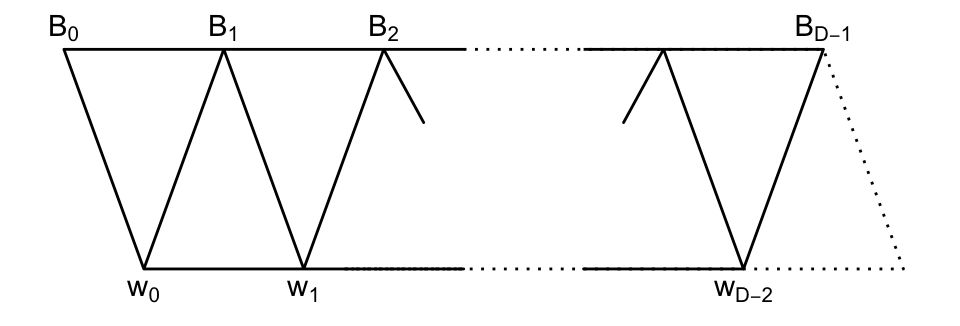
\includegraphics{t-algebra_files/figure-latex/unnamed-chunk-10-1} \end{center}

Now,
\[\Psi(x,y) = \Psi(x,w) = \Psi(x,z)\]
from the first case.
\end{proof}

\begin{lemma}
\protect\hypertarget{lem:aplus-aminus}{}\label{lem:aplus-aminus}With the above notation, the following hold.

\((i)\) \(A^+: = R^{-1}E^*_2A_2E^*_1 - \Psi E^*_1\), and

\((ii)\) \(A^- = \tilde{A}A^+ - \left(\frac{a_2}{c_2}-\Psi\right)E^*_1 + \Psi(\tilde{J} - \tilde{A} - E^*_1)\)

are both generalized adjacency matrices for the subgraph induced on the first subconstituent with respect to \(x\).

Moreover, \(A^+\), \(A^-\) have \(0\) diagonal.
\end{lemma}

\begin{proof}
Pick vertices \(y,z\in X\) such that \(\partial(x,y) = \partial(x,z) = 1\).

Show that \(A^+_{yz}\), \(A^-_{yz}\) are both \(0\) if \(\partial(y,z) = 0\) or \(2\).

Since \(A^+_{yz} = R^{-1}E^*_2A_2E^*_1\hat{y} - \Psi E^*_1\hat{y} = \delta^+_{11}\),
\[A^+_{yz} = \langle A^+\hat{y}, \hat{z}\rangle = \langle \delta^+_{11},\hat{z}\rangle = 0,\]
if \(\partial(y,z) = 0\) or \(2\).

Since
\begin{align}
A^-\hat{y} & = \tilde{A}A^+\hat{y} - \left(\frac{a_2}{c_2}-\Psi\right)E^*_1\hat{y} + \Psi(\tilde{J} - \tilde{A} - E^*_1)\hat{y}\\
& = \tilde{A}\delta^+_{11} - \left(\frac{a_2}{c_2}-\Psi\right)\hat{y} + \Psi\delta_{12}\\
& = \delta^-_{11},
\end{align}
\[A^-_{yz} = \langle A^-\hat{y}, \hat{z}\rangle = \langle \delta^-_{11}, \hat{z}\rangle = 0,\]
if \(\partial(y,z) = 0\) or \(2\).

Since \(E^*_1TE^*_1 = \mathrm{Span}(\tilde{J},E^*_1, \tilde{A}, \tilde{A}^2, \ldots)\) by Lemma \ref{lem:e1starte1star}.

\(A^+, A^-\) are both generalized matrices for the adjacency subgraph induced on the first subconstituent concerning \(x\).
\end{proof}

Similarly,
\[E^*_1TE^*_1 \ni \tilde{J}, E^*_1, \tilde{A}, A^+, A^-,\]
and \(\dim E^*_1TE^*_1 \leq 5\).

Fact: With the above assumption,
\[E^*_1TE^*_1 = \mathrm{Span}(\tilde{J}, E^*_1, \tilde{A}, A^+, A^-)\]
(may not be independent).

\begin{lemma}
\protect\hypertarget{lem:tyx-equals-txy}{}\label{lem:tyx-equals-txy}If \(\partial(x,y) = 1\), then
\[T(y)\hat{y} = T(x)\hat{y}.\]
\end{lemma}

\begin{proof}
\begin{align}
T(x)\hat{x} & = T(x)E^*_1\hat{y}\\
& = M(E^*_0+E^*_1)T(x)E^*_1\hat{y} \quad (\text{as $\Gamma$ is thin})\\
& = M\hat{x} + ME^*_1TE^*_1\hat{y}\\
& = M\hat{x} + M\mathrm{Span}(\tilde{J}, E^*_1, \tilde{A}, A^+, A^-)\hat{y}\\
& = M\hat{x} + M\mathrm{Span}(\delta_{12}+\delta_{11}+\delta_{10}, \delta_{10}, \delta_{11}, \delta^+_{11}, \delta^-_{11})\\
& = M\mathrm{Span}(\delta_{01}, \delta_{10}, \delta_{11}, \delta^+_{11}, \delta^-_{11}).
\end{align}

But the identity of these conditions does not change if we interchange \(x\) and \(y\).

Hence,
\[T(y)\hat{y} = T(x)\hat{y}.\]
This proves the lemma.
\end{proof}

\hypertarget{lec40}{%
\chapter{Structure of 1-Thin DRG}\label{lec40}}

\textbf{Friday, May 7, 1993}

\begin{lemma}
\protect\hypertarget{lem:endpoint-at-most-one}{}\label{lem:endpoint-at-most-one}With the above notation, let \(W\) denota a thin irreducible \(T\)-module of endpoint \(0\) or \(1\). Pick \(0\neq v\in E^*_1V\). Then the following hold.

\((i)\) Eigenvalue for \(\tilde{J}\) is \(0\) if \(r(W)=1\), and \(k\) if \(r(W) = 0\).

\((ii)\) Eigenvalue for \(E^*_1\) is \(1\) if \(r(W)=1\), and \(1\) if \(r(W) = 0\).

\((iii)\) Eigenvalue for \(\tilde{A}\) is \(a_0(W)\) if \(r(W)=1\), and \(a_1\) if \(r(W) = 0\).

\((iv)\) Eigenvalue for \(A^+\) is \(a^+(W) = \frac{\gamma_1}{c_2}-1-\Psi\) if \(r(W)=1\), and \(\frac{a_2}{c_2}-\Psi\) if \(r(W) = 0\).

\((v)\) Eigenvalue for \(A^-\) is \(a^-(W) = a_0(W)\left(\frac{\gamma_1}{c_2}-1-2\Psi\right)-\frac{a_2}{c_2}\) if \(r(W)=1\),

where
\[\gamma_0 = 1+a_0(W), \text{ and } \gamma_1 = \frac{c_2b_2\gamma_0}{b_1+\gamma_0(a_1+2-c_2)-\gamma^2_0}\]
as in Theorem \ref{lem:thin-endpoint1}. (The eigenvalue for \(A^-\) on \(v\) will be discussed later in this lecture.)
\end{lemma}

\begin{proof}
\leavevmode

\((i)-(iii)\) Clear.

\((iv)\) We have

\begin{align}
A^+ & = R^{-1}E^*_2A_2E^*_1 - \Psi E^*_1,\\
A_2 & = \frac{A^2-a_1A - kI}{c_2},\\
E^*_2A_2E^*_1 & = E^*_2\left(\frac{A^2-a_1A - kI}{c_2}\right)E^*_1\\
& = \frac{1}{c_2}(RF + FR - a_1R)E^*_1.
\end{align}

If \(r(W) = 1\),
\begin{align}
A^+v & = \frac{1}{c_2}(R^{-1}RFv + R^{-1}FRv - a_1R^{-1}Rv) - \Psi v\\
& = \frac{1}{c_2}(R^{-1}Ra_0(W)v + R^{-1}a_1(W)Rv - a_1R^{-1}Rv) - \Psi v\\
& = \frac{1}{c_2}\left(a_0(W) + a_1(W) - a_1) - \Psi\right)v.
\end{align}
But,
\[a_1(W) = \gamma_1 - \gamma_0 + a_1 + 1 - c_2, \quad \gamma_0 = a_0(W) + 1\]
by Theorem \ref{thm:endpoint1}.

So,
\begin{align}
A^+v & = \left(\frac{1}{c_2}(a_0(W) + \gamma_1 - \gamma_0 + a_1 + 1 - c_2 - a_1) - \Psi)\right)v\\
& = \left(\frac{\gamma_1}{c_2}-1-\Psi\right)v.
\end{align}

If \(r(W) = 0\),
\begin{align}
A^+v & = \frac{1}{c_2}(R^{-1}RFv + R^{-1}FRv - a_1R^{-1}Rv) - \Psi v\\
& = \frac{1}{c_2}(R^{-1}Ra_1v + R^{-1}a_2Rv - a_1R^{-1}Rv) - \Psi v\\
& = \left(\frac{a_2}{c_2}-\Psi\right)v.
\end{align}

\((v)\) Immediate from \((iv)\), and

\[A^- = \tilde{A}A^+ - \left(\frac{a_2}{c_2} - \Psi\right)E^*_1 + \Psi(\tilde{J}-\tilde{A}-E^*_1).\]

\textbf{HS MEMO}

If \(r(W) =1\),
\begin{align}
A^-v & = \left(a_0(W)\left(\frac{\gamma_1}{c_2}-1-\Psi\right) - \left(\frac{c_2}{a_2}-\Psi\right) + \Psi(-a_0(W)-1)\right) v\\
& = \left(a_0(W)\left(\frac{\gamma_1}{c_2}-1-2\Psi\right) - \frac{c_2}{a_2}\right)v.
\end{align}
If \(r(W) = 0\),
\begin{align}
A^-v & = \left(a_1\left(\frac{a_2}{c_2}-\Psi\right) - \left(\frac{a_2}{c_2}-\Psi\right) + \Psi(k-a_1-1)\right) v\\
& = \left((a_1-1)\frac{a_2}{c_2}+ (k-2a_1)\Psi\right)v.
\end{align}

This completes the proof.

\end{proof}

Let \(W_1, W_2, W_3, W_4\) denote \(4\) possible isomorphism classes of \(T\)-modules of endpoint \(1\). Then \(a_0(W_1), a_0(W_2), a_0(W_3), a_0(W_4)\) are roots of a fourth degree polynomial whose coefficients are determined from intersection numbers of \(\Gamma\).

So, \(a_0(W_1), a_0(W_2), a_0(W_3), a_0(W_4)\) are determined by intersection numbers.

Let \(\widetilde{m_i}\) denote the multiplicity of \(W_i\) \((1\leq i\leq 4\)), which is equal to the multiplicity of \(a_0(W)\) as eigenvalue \(1\) of \(\tilde{A}|_{(E^*_1V)_{new}}\).

\begin{lemma}
\protect\hypertarget{lem:tilde-mi}{}\label{lem:tilde-mi}

With the above notation, we have the following.

\((i)\) \(\tilde{m}_1\), \(\tilde{m}_2\), \(\tilde{m}_3\), \(\tilde{m}_4\) are determined from intersection numbers and \(\Psi\).

\((ii)\) \(\tilde{m}_i\) is independent of vertex \(x\). \((1\leq i\leq 4)\).

\((iii)\) \(\ell:= \dim E^*_1TE^*_1\) is independent of \(x\).

\end{lemma}

\begin{proof}
\leavevmode

\((i)\) Let \(e_i\in E^*_1TE^*_1\) \((1\leq i\leq 4)\) denote the orthogonal projection on to the maximal eigenspace of \((E^*_1V)_{new}\) corresponding to \(\lambda_i\). (\(e=0\) if and only if \(\lambda_i\) does not appear.) Set

\[e_0 = \frac{1}{k}\tilde{J}.\]
Then eigenvalues for each \(e_1, e_1, e_3, e_4\) are as follows.
\[\begin{array}{|c|ccccc|} \hline
\text{} & e_0 & e_1 & e_2 & e_3 & e_4\\
\hline
\tilde{J} & k & 0 & 0 & 0 & 0\\
E^*_1 & 1 & 1 & 1 & 1 & 1 \\
\tilde{A} & a_1 & a_0(W_1) & a_0(W_2) & a_0(W_3) & a_0(W_4)\\
A^+ & \frac{a_2}{c_2}-\Psi & a^+(W_1)  & a^+(W_2)  & a^+(W_3)  & a^+(W_4)\\
A^- & \star & a^-(W_1)  & a^-(W_2)  & a^-(W_3)  & a^-(W_4)\\
\hline
\end{array}\]

Observe that \(e^2_i = e_i\), \(\mathrm{trace} \:e_i = \mathrm{rank}\:e_i = \tilde{m}_i\) \((1\leq i\leq 4)\), and \(\mathrm{trace}\: e_0 = \mathrm{rank}\:e_0 = 1\).

By taking the trace of \(\tilde{J}, E^*_1, \tilde{A}, A^+, A^-\), we have
\begin{align}
k & = k,\\
k & = 1 + \tilde{m}_1 + \tilde{m}_2 + \tilde{m}_3 + \tilde{m}_4,\\
0 & = a_1 + a_0(W_1)\tilde{m}_1 + a_0(W_2)\tilde{m}_2 + a_0(W_3)\tilde{m}_3 + a_0(W_4)\tilde{m}_4,\\
0 & = \left(\frac{a_2}{c_2}-\Psi\right) + a^+(W_1)\tilde{m}_1 + a^+(W_2)\tilde{m}_2 + a^+(W_3)\tilde{m}_3 + a^+(W_4)\tilde{m}_4,\\
0 & = \left(\star\right) + a^-(W_1)\tilde{m}_1 + a^-(W_2)\tilde{m}_2 + a^-(W_3)\tilde{m}_3 + a^-(W_4)\tilde{m}_4.
\end{align}

The coefficient matrix for \(\tilde{m}_1,\tilde{m}_2, \tilde{m}_3,\tilde{m}_4\) is nonsingular (this is what you need to check and show).

\textbf{HS MEMO}

Complutation is not completed.

\((ii)\) \(\Psi\) is independent of base vertex \(x\).

\((iii)\) We have

\begin{align}
\dim E^*_1TE^*_1 & = |\{i\mid 1\leq i\leq 4, \; e_i\neq 0\}| + 1\\
& = |\{i\mid 1\leq i\leq 4, \; \tilde{m}_i\neq 0\}| + 1.
\end{align}

This completes the proof of the lemma.

\end{proof}

Let \(\Gamma = (X, E)\) be thin distance regular of diameter \(D\geq 5\), and \(Q\)-polynomial with respect to \(E_0, E_1, \ldots, E_D\).

Fix vertices \(x,y\in X\) with \(\partial(x,y) = 1\),
\[E^*_{ij} \equiv E^*_i(x)E^*_j(y), \quad \delta_{ij} = E^*_{ij}\delta.\]
We saw
\[T(x)\hat{y} = T(y)\hat{x}.\]
Hence,
\[H := T(x)\hat{y} = T(y)\hat{x}\]
is a \(T(x,y)\) module.
\(T(x,y) \subseteq \mathrm{Mat}_X(\mathbb{C})\) is generated by \(M\), \(M^*(x)\), \(M^*(y)\).

\begin{lemma}
\protect\hypertarget{lem:h}{}\label{lem:h}

With the above notation, we have the following.

\((i)\) \(E^*_{i,i+1}H = \mathrm{Span}(\delta_{i,i+1}) \quad (0\leq i\leq D-1)\).

\((ii)\) \(E^*_{i+1,i}H = \mathrm{Span}(\delta_{i+1,i}) \quad (0\leq i\leq D-1)\).

\((iii)\) \(E^*_{i,i}H = \ell-2 \leq 3 \quad (1\leq i\leq D-1)\).

\end{lemma}

\begin{proof}
\leavevmode

\((i)\) \(\supseteq\): We have

\[\delta_{i,i+1} = E^*_iA_{i+1}\hat{y} \in T(x)\hat{y} = H.\]

\(\subseteq\): Pick \(h\in E^*_{i,i+1}H\). Then \(h = R^{i-1}v\), where \(v = (R^{-1})^{i-1}h\in E^*_1V\).

So, \(v\in \mathrm{Span}(\delta_{12}, \delta_{11}, \delta_{10}, \delta^+_{11}, \delta^-_{11})\).

\textbf{HS MEMO}

\begin{align}
v &\in E^*_1V \cap T(x)\hat{y}\\
& = E^*_1T(x)E^*_1\hat{y}\\
& = \mathrm{Span}(\tilde{J}, E^*_1, \tilde{A}, A^+, A^-)\hat{y}\\
& = \mathrm{Span}(\delta_{10}+ \delta_{11}+ \delta_{12}, \delta_{10}, \delta_{11}, \delta^+_{11}, \delta^-_{11})\\
& = \mathrm{Span}(\delta_{10}, \delta_{11},  \delta_{12}, \delta^+_{11}, \delta^-_{11}).
\end{align}

Hence, there exists \(\alpha \in \mathbb{C}\) such that
\[v-\alpha \delta_{12}  \in \mathrm{Span}(\delta_{10}, \delta_{11}, \delta^+_{11}, \delta^-_{11}) = E^*_{11}H + E^*_{10}H.\]
So,
\[v-\alpha(\delta_{12} + \delta_{11} + \delta_{10}) \in E^*_{11}H + E^*_{10}H.\]
\begin{align}
E^*_{ii}H + E^*_{i,i-1}H & \ni R^{i-1}(v-\alpha(\delta_{12}+\delta_{11}+\delta_{10}))\\
& = h - \alpha'(\delta_{i,i+1}+\delta_{ii}+\delta_{i,i-1}).
\end{align}
Hence,
\[h-\alpha'\delta_{i,i+1}\in (E^*_{ii}H + E^*_{i,i-1}H)\cap E^*_{i,i+1}H.\]
Thus,
\[h = \alpha'\delta_{i,i+1} \in \mathrm{Span}(\delta_{i,i+1}).\]

\((ii)\) By symmetry, we have the assertion.

\((iii)\) \(E^*_i H = E^*_{i,i+1}H + E^*_{i,i}H + E^*_{i,i-1}H\), and \(\dim E^*_iH = \ell\), \(\dim E^*_{i,i+1}H =1\), and \(\dim E^*_{i,i-1}H = 1\).

Hence, \(\dim E^*_{i,i}H = \ell -2\).

\end{proof}

\textbf{HS MEMO}

Since \(H = T(x)\hat{y} \subseteq T(x)E^*_{1}(x)V\), and
\[(R^{-1})^{i-1}: E^*_iH \to E^*_1H\]
is one-to-one and onto if \(i\leq D\).

\begin{theorem}
\protect\hypertarget{thm:zi}{}\label{thm:zi}Let \(\Gamma = (X, E)\) be thin distance regular of diameter \(D\geq 5\), and \(Q\)-polynomial with respect to \(E_0, E_1, \ldots, E_D\).

Pick \(i\) \((2\leq i\leq D)\), and pick \(x, y, z\in X\) such that \(\partial(x,y) =1\), \(\partial(y,z) = i-1\), \(\partial(x,z) = i\).

Then,
\[z_i = |\{w\mid w\in W, \partial(x,w) =1, \partial(y,w)=1, \partial(z,w)=i-1\}|\]
is independent of \(x, y, z\).
\end{theorem}

\begin{proof}
Observe that \(z_i\) is the \(zx\) entry in
\[\Delta = E^*_{i-1}(y)A_{i-1}E^*_1(y)AE^*_1(y)\]
as
\[\Delta \hat{x} = \sum_{z\in X, \partial(x,z)=i, \partial(y,z)=i-1}z_i(x,y,z)\hat{z}.\]
Hence, \(z_i(x,y,z)\) is independent of \(z\).

So, \(z_i(x,y,z)\) is determined by intersection numbers and \(\Psi = \Psi(x,y)\), which is independent of \(x, y\) as well.
\end{proof}

\hypertarget{appendix-appendix}{%
\appendix}


\hypertarget{prob}{%
\chapter{Open Problems}\label{prob}}

\textbf{Some Open Problems Concerning Distance-Regular Graphs, the Thin Condition, and the \(Q\)-Polynomial Property}

Paul Terwilliger

\hfill\break

The questions below are unsolved as of May, 1993 (to my knowledge). A complete solution (or even a significant partial solution in some cases) to any one of these problems would be publishable. I have tried to estimate the level of difficulty of each problem listed below. A \(\star\) means I believe the problem is relatively easy in the sense that it can be solved using ideas from the course. There are no conceptual gaps to overcome that I am aware of (but the calculations might be quite difficult, however!). A \(\star\star\)\(\star\star\) means I have no idea how to begin to attack the problem. I am only mentioning problems of this kind to give you an idea about what is known in this field.

\hfill\break
\emph{Dist}: \(\Gamma\) is distance-transitive.

\hfill\break
\emph{Q}: \(\Gamma\) is \(Q\)-polynomial with respect to the ordering \(E_0, E_1, \ldots, E_D\) of the primitive idempotents.

\hfill\break
\emph{Bip}: \(\Gamma\) is bipartite.

\hfill\break
\emph{Th}: \(\Gamma\) is thin (over the field of complex numbers).

\hfill\break
\emph{Few1}: The subgraph induced on the first subconstituent of \(\Gamma\) with respect to \(x\) has at most \(5\) distince eigenvalues.

\hfill\break
\emph{Few2}: The subgraph induced on the second subconstituent of \(\Gamma\) with respect to \(x\) has at most \(16\) distinct eigenvalues.

\hfill\break
\emph{Z}: For all integers \(i\) \((2\leq i\leq D)\), and all triples \(u, v, w\) (\(u,v, w\in X)\) such that \(\partial(u,v) = 1\), \(\partial(v,w) = i-1\), and \(\partial(v,w) = i\), the number

\[z_i:=|\{y\mid y\in X, \partial(y,u) = \partial(y,v) =1, \partial(y,w) = i-1\}|\]
is a constant that does not depend on \(u,v,w\).

The following implications are known:

\(\quad\) \emph{Q} \(+\) \emph{Bip} \(\to\) \emph{TH}, \(\quad\) \emph{Q} \(+\) \emph{TH} \(\to\) \emph{Few1}, \emph{Few2}, \emph{Z}.

\((1)\) \(\star\star\)\(\star\star\) Classify all the distance-regular graphs (with sufficiently large diameter). If necessary, assume some combination of the above properties. (My personal goal is to classify all the graphs \(\Gamma\) satisfying \emph{Q}, \emph{TH}. I expect this will take a number of years.)

\hfill\break
\((2)\) \(\star\star\) Assume \emph{Q}, \emph{Bip}, and classify \(\Gamma\).

\hfill\break
\((3)\) \(\star\) Find generalization to the theorems of the course for non-regular, bipartite distance-regular graphs.

\hfill\break
\((4)\) \(\star\) Assume, \emph{Q}, and let \(W\) denote an irreducible \(T\)-module with endpoint \(1\) that is not thin. Find a nice basis for \(W\) and find the matrices representing the adjacency matrix \(A\) and the dual adjacency matrix \(A^*\) with respect to this basis. Perhaps assume classical parameters. Theorem \ref{thm:rfl-relations}, and Lemma \ref{lem:inverse-of-r} should be useful.

\hfill\break
\((5)\) \(\star\) Is it true that \(\Gamma\) is thin over the field of complex numbers if and only if \(\Gamma\) is thin over the field of real numbers? What does it mean for \(\Gamma\) to be thin over the field of rational numbers? The examples suggest that if \(\Gamma\) is thin over the complex numbers then it is already thin over the rational numbers. If this is true, it would be nice to have a proof. For the moment, suppose it is not true. Assume \(\Gamma\) is thin over the field of complex numbers, and define the \emph{splitting field} of \(\Gamma\) to be the minimal extension of the rational field over which \(\Gamma\) is thin. Then the elements of the Galois group of the splitting field act on the standard module, and permute the isomorphism classes of irreducible \(T\)-modules. How are the isomorphism classes of \(T\)-modules involved related? Can the permutations be nontrivial?

\hfill\break
\((6)\) \(\star\star\) Assume \emph{Q}, and assume there is a second \(Q\)-polynomial ordering of the primitive idempotent. Prove \emph{TH}. I believe in this case the first subconstituent has at most \(4\) distinct eigenvalues, and the constant \(\Psi\) from class if determined by the intersection numbers. It may be possible to classify all such \(\Gamma\).

\hfill\break
\((7)\) \(\star\star\) Assume \emph{Q}, and assume there is a second \(P\)-polynomial ordering of the distance matrices. I believe the same thing happens as in \((6)\) above.

\hfill\break
\((8)\) \(\star\star\) A path \(y = y_0, y_1, \ldots, y_t = z\) in \(\Gamma\) is said to be \emph{geodetic} whenever \(\partial(y,z)=t\). Let us say a subset \(\Delta\) of \(X\) is \emph{geodetically closed} whenever all vertices on all geodetic paths with endpoints in \(\Delta\) are also in \(\Delta\). For any vertices \(y,z\in X\), observe there exists a unique minimal geodetically closed subset containing \(y,z\), denoted \([yz]\).

If the diameter of \([yz]\) equals \(\partial(y,z)\), we say \([yz]\) is a subspace. Furthermore, show the subgraph induced on \([yz]\) is distance-regular, and satisfies \emph{Q}, \emph{TH}. If this proves not to be the case, find a simple additional assumption on \(\Gamma\) under which it is true. (It seems to hold for the known examples). I believe these subspaces are the key to an eventual classification of the graphs satisfying \emph{Q}, \emph{TH} (and possibly all distance-regular graphs with sufficiently large diameter). In the examples, the partially ordered set of all subspaces, ordered by reverse inclusion, is some classical geometry. There are many classification theorems in the area of finite projective geometry. My hope is that given any \(\Gamma\), the partially ordered set of all subspaces is some highly regular geometry that can be classified using one of these theorems, leading us to a classification of the original \(\Gamma\). (By the way, I intend to explore this area in the course I am teaching next fall on partiallly ordered sets).

\hfill\break
\((9)\) \(\star\star\) Assume \emph{Q}, \emph{TH}. Find a nice basis for \(E^*_2TE^*_2\) in a way that generalized what we did in class for \(E^*_1TE^*_1\).

\hfill\break
\((10)\) \(\star\) Assume \emph{B}, \emph{TH}, and that the dimension of \(E^*_2TE^*_2\) is at most \(4\). Show that \emph{Q} holds. Find a nice basis for \(E^*_2TE^*_2\).

\hfill\break
\((11)\) It is not hard to show that in general

\begin{align}
c_i\geq c_{i-1} & \quad (1\leq i\leq D),\\
b_i \leq b_{i-1} & \quad (0\leq i\leq D-1).
\end{align}
It is known that if \(\Gamma\) has at least one cyle \(y1, y2, y3, y4, y1\) such that \(\partial(y1,y3) = \partial(y2,y4)=2\) then
\[c_i - c_{i-1} + b_{i-1} - b_i \geq a_1 + 2 \quad (1\leq i\leq D).\]
This bound has proved to be quite fndamental. For example, the graphs \(\Gamma\) where equality holds for all \(i\) all satisfy \emph{Q}, and in fact they are precisely the graphs of type IIA or IIC (refereng to p.10, 11 in the thick paper I handed out in class). These graphs have all been classified. I have some papers describing some more general bounds of the above sort, but they are unsatisfactory in the sense that the class of graphs for which equality is attained is not interesting, and may even be empty. Hence one problem (\(\star\star\)) is to find a bound that controls the growth of the \(c_i\)'s and the decrease of the \(b_i\)'s, where equality is attained for some nice, large class of graphs. Ideally, this class would contain all the known examples of \(\Gamma\) with sufficiently large diameter, or perhaps all the graphs \(\Gamma\) satisfying \emph{Q} \(+\) \emph{TH}. Specific proble (\(\star\)): Assume \emph{Z} and redo the arguments in the above-mentioned papers. Dramatic improvements in the bounds obtained are expected (I did not realise the significance of \emph{Z} and redo the arguments in the above-mentioned papers). Since \emph{Q} \(+\) \emph{TH} \(\to\) \emph{Z}, the new bounds are expected to give important feasibility conditions on the intersection numbers of any \(\Gamma\) satisfying \emph{Q} and \emph{TH}.

\hfill\break
\((12)\) \(\star\) Explore the class of graphs that are \(Q\)-polynomial with respect to each vertex. but not assumed to be distance-regular. Are these graphs in fact distance-regular or bi-distance-regular? (This result would be very esthetically pleasing to me, since as we have seen, the sibling property of being thin does not imply distance-regularity or bi-distance-regularity). If the answer to the above question is ``no'', just what sort of regularity do these graphs have? For a graph that is \(Q\)-polynomial with respect to each vertex, how must the orderings of the primitive idempotents associated with adjacent vertices be related? Is it possible for a distance-regular graph to be \(Q\)-polynomial with respect to each vertex, but still not be \(Q\)-polynomial? (This is a completely new area. Up until now, the \(Q\)-polynomial property was only defined for distance-regular graphs.)

\hfill\break
\((13)\) \(\star\star\) To what extent do the polynomial relations on \(R\), \(L\), \(F\) given in Theorem \ref{thm:rfl-relations} actually characterize the \(Q\)-polynomial property? For example, suppose

\(\quad (i)\) \(L^2FE^*_i, LFLE^*_i, FL^2E^*_i, L^2E^*_i\) are linearly dependent for all \(i\) \((2\leq i\leq D)\).

\(\quad (ii)\) \(FLRE^*_i, FRLE^*_i\) are linearly dependent for all \(i\) \((0\leq i\leq D)\), and

\(\quad (iii)\) \(RL^2E^*_i, LRLE^*_i, L^2RE^*_i, LF^2E^*_i, FLFE^*_i, LFE^*_i, F^2LE^*_i, FLE^*_i, LE^*_i\) are linearly dependent, for all \(i\) \((1\leq i \leq D)\).

Then does \emph{Q} hold? what if we assume \emph{TH}? If not, what other graphs can one get? are they ``almost'' \(Q\)-polynomial in some sense (pserhaps many Krein parameters vanish, but not quite enough to imply \(Q\)). What is the essential assumption about the coefficients in the above dependencies that is needed to insure \emph{Q}.

\hfill\break
\((14)\) \(\star\star\)\(\star\) Assume \emph{Q} and \emph{TH}. Find the abstract structure of the Norton algebra \(N\). My intuition says that this structure can be computed in terms of the intersection numbers and a small list of additional parameters such as \(\psi\). The examples suggest that \(N\) is ``almost associative'' in some sense. Specific problem (\(\star\)) Find the precise structure of the Norton algebra for the examples \(J(d,n)\), \(J_q(d,n)\), \(\ldots\), and find some pattern. The dual of Theorem \ref{thm:rfl-relations} is relevent to this problem. My intuition says that the idempotents of \(N\) should correspond to the subspaces of \(\Gamma\) referred to in problem 8, and that somehow the multiplication operation in \(N\) should be related to the meet and join operations in the geometry of subspaces referred to in that problem.

\hfill\break
\((15)\) \(\star\star\) Assume \emph{Q} and \emph{TH}, and pick \(y\in X\). Show

\[T(x)\hat{y} = T(y)\hat{x}.\]
(I can show this for \(\partial(x,y)=1\).) If the above line holds, then apparently \(H:=T(x)\hat{y} = T(y)\hat{x}\) is a module for the algebra \(T(x,y)\) generated by the Bose-Mesner algebra \(M\), the dual Bose-Mesner algebra \(M^*(x)\), and \(M^*(y)\). Observe the elements of \(M^*(x)\), \(M^*(y)\) mutually commute, and in fact that the maximal common engenspaces of \(M^*(x)\), \(M^*(y)\) are the \(E^*_{ij}V\) \((0\leq i,j\leq D)\), where \(E^*_{ij} = E^*_i(x)E^*_j(y)\). Find a nice orthogonal basis for each \(E^*_{ij}H\). Observe the union \(B\) of these bases is a basis for \(H\). Find the matrices representing \(A\), \(A^*(x)\), \(A^*(y)\) with respect to \(B\). Choose \(B\) so that the entries in these matrices are nice, factorable expressions in the intersection numbers and whatever other parameters are needed. In the case \(\partial(x,y)=1\), these entries can be deteermined from the intersection numbers and the parameter \(\psi\). If \(\partial(x,y)\geq 2\), presumably there are some more free parameters analoguous to \(\psi\) that play a role. My intuition says that as a \(T(x,y)\)-module, \(H\) is determined from the intersection numbers of \(\Gamma\) and \(t\) free parameters, where \(t = \partial(x,y)\).

\hfill\break
\((16)\) \(\star\star\) Does \emph{TH} and \emph{Few1} imply \emph{Z}? If not, what extra assumption is needes?

\hfill\break
\((17)\) \(\star\star\) Does \emph{TH}, \emph{Few1}, \emph{Few2}, imply \emph{Q}? If not, what extra assumption is needed?

\hfill\break
\((18)\) \(\star\star\) Let \(\Gamma\) be an arbitrary grarph, not assumed to be distance-regular. Conjecture: \(\Gamma\) is thin if and only if for all integers \(i,j,k\), and all vertices \(x,y,z\in X\) such that \(\partial(x,y) = \partial(x,z) = i\), the number of vertices \(w\in X\) with \(\partial(w,x) = j\), \(\partial(w,y) = 1\), \(\partial(w,z) = k\) equals the number of vertices \(w'\in X\) with \(\partial(w',x) = j\), \(\partial(w',z)=1\), \(\partial(w',y)=k\). If \(\Gamma\) assumed to be distance-regular, then the conjecrure is true and there is a long proof in the thick paper I handed out in class (Theorem 5.1 (iii)) . A short, slick proof (assuming distance-regularity or not) is very much needed. If the conjecture turns out not to be true in the bi-distance-regular case, find some similar combinatorial characterization of the thin property.

There are a number of additional problems in section 7 of the thick paper I handed out in class. Essentially all the known examples of thin, \(Q\)-polynomial distance-regular graphs are listed in section 6 of that paper.

For each of the above problems, I have a good deal of background information to communicate, but unfortunately in most cases it is not in published form! If you tell me what problem you want to focus on, I can tailor a series of lectures this summer towards communicating what I know on the subject. But one key point: Often ``I don't know what I know''. If you are constantly asking probing questions of me it makes my job a lot easier: it often reminds me of information that is relevant that I had forgotten, or that I had forgotten was relevant.

\hypertarget{table}{%
\chapter{Comparison Table}\label{table}}

We list Definitions, Theorems, Lemmas, etc. with the numbers in the original handwritten note.

\begin{longtable}[]{@{}
  >{\raggedright\arraybackslash}p{(\columnwidth - 4\tabcolsep) * \real{0.1154}}
  >{\raggedright\arraybackslash}p{(\columnwidth - 4\tabcolsep) * \real{0.6795}}
  >{\raggedright\arraybackslash}p{(\columnwidth - 4\tabcolsep) * \real{0.2051}}@{}}
\toprule()
\begin{minipage}[b]{\linewidth}\raggedright
Chapter
\end{minipage} & \begin{minipage}[b]{\linewidth}\raggedright
New Numbering
\end{minipage} & \begin{minipage}[b]{\linewidth}\raggedright
Old Numbering
\end{minipage} \\
\midrule()
\endhead
1 & Example \ref{exm:four-vertex-graph} & Example \\
& Example \ref{exm:adjacency-matrix} & Example \\
& Definition \ref{def:regular} & Definition \\
& Lemma \ref{lem:largestev} & Lemma 1 \\
& Definition \ref{def:path} & Definition \\
& Definition \ref{def:distance} & Definition \\
& Definition \ref{def:connected} & Definition \\
& Definition \ref{def:diameter} & Definition \\
& Definition \ref{def:t-algebra} & Definition \\
& Definition \ref{def:module} & Definition \\
& Lemma \ref{lem:complete-reducibility} & Lemma 2 \\
2 & Definition \ref{def:reducible} & Definition \\
& Definition \ref{def:bipartite-mat} & Definition \\
& Theorem \ref{thm:pf} & Theorem 3 \\
& Lemma \ref{lem:pfl} & Lemma 4 \\
& Definition \ref{def:bipartite} & Definition \\
& Corollary \ref{cor:spec} & Corollary 5 \\
3 & Definition \ref{def:isom} & Definition \\
& Definition \ref{def:auto} & Definition \\
& Definition \ref{def:transitive} & Definition \\
& Definition \ref{def:cayley} & Definition \\
& Example \ref{exm:cyclic6} & Example \\
& Example \ref{exm:k6minus1} & Example \\
& Example \ref{exm:d6} & Example \\
& Theorem \ref{thm:cayley-graph} & Theorem 6 \\
& Definition \ref{def:character} & Definition \\
& Example \ref{exm:cyclic3} & Example \\
& Lemma \ref{lem:charactergroup} & Lemma 7 \\
4 & Theorem \ref{thm:charcter-group} & Theorem 8 \\
& Example \ref{exm:character-cyclic6} & Example \\
& Example \ref{exm:hd2} & Example \\
& Definition \ref{def:rd} & Definition \\
& Lemma \ref{lem:irreducible} & Lemma 9 \\
5 & Definition \ref{def:isomorphic-modules} & Definition \\
& Theorem \ref{thm:hd2-modules} & Theorem 10 \\
6 & Theorem \ref{thm:hd2-modules2} & Theorem 11 \\
& Definition \ref{def:thin-dualthin} & Definition \\
& Definition \ref{def:q-polynomial-graph} & Definition \\
7 & Definition \ref{def:johnson} & Definition \\
& Example \ref{exm:j42} & Example \\
& Lemma \ref{lem:ev-johnson} & Lemma 12 \\
& Theorem \ref{thm:thin-condition} & Theorem 13 \\
8 & Lemma \ref{lem:property-g} & Lemma 14 \\
9 & Lemma \ref{lem:thin-module-structure} & Lemma 15 \\
& Corollary \ref{cor:thin-is-dualthin} & Corollary 16 \\
& Lemma \ref{lem:measure-wi} & Lemma 17 \\
& Definiton \ref{def:measure} & Definition \\
10 & Lemma \ref{lem:orthogonality} & Lemma 18 \\
& Lemma \ref{lem:determined-by-m} & Lemma 19 \\
& Corollary \ref{cor:isomorphic} & Corollary 20 \\
11 & Lemma \ref{lem:principal-module} & Lemma 21 \\
& Lemma \ref{lem:baiparite-principal} & Lemma 22 \\
12 & Lemma \ref{lem:distance-reguarity} & Lemma 23 \\
& Theorem \ref{thm:two-thin-modules} & Theorem 24 \\
13 & Lemma \ref{lem:two-principal-modules} & Lemma 25 \\
& Theorem \ref{thm:distance-regular-x} & Theorem 26 \\
& Proposition \ref{prp:dim-diameter} & Proposition 27 \\
14 & Lemma \ref{lem:basic-data} & Lemma 28 \\
& Lemma \ref{lem:thin-endpoint1} & Lemma 29 \\
15 & Definition \ref{def:complete-graph} & Definition \\
& Lemma \ref{lem:sedond-and-largest-ev} & Lemma 30 \\
16 & Definition \ref{def:ith-incidence} & Definition \\
& Lemma \ref{lem:incidence-matrices} & Lemma 31 \\
& Theorem \ref{thm:endpoint1} & Theorem 32 \\
& Lemma \ref{lem:aixigi} & Lemma 33* \\
17 & Definition \ref{def:association-scheme} & Definition \\
& Definition \ref{def:incidencemat-of-as} & Definition \\
& Example \ref{exm:dr} & Example 1 \\
& Example \ref{exm:gen-tr} & Example 2 \\
& Exercise \ref{exr:gen-tr-case} & Exercise \\
& Example \ref{exm:centralizer-alg} & Example 3 \\
18 & Lemma \ref{lem:dr-scheme} & Lemma 33 \\
19 & Lemma \ref{lem:ei} & Lemma 34 \\
& Definition \ref{def:dual-bose-mesner} & Definition: \\
20 & Lemma \ref{lem:pij-qij} & Lemma 34-a \\
& Lemma \ref{lem:phijqhij} & Lemma 34-b \\
& Lemma \ref{lem:vanishing-condition} & Lemma 35 \\
& Corollary \ref{cor:qhij} & Corollary 36 \\
& Lemma \ref{lem:vector-function-product} & Lemma 37 \\
21 & Lemma \ref{lem:norton-algebra} & Lemma 38 \\
& Lemma \ref{lem:autom-of-norton-algebra} & Lemma 39 \\
22 & Lemma \ref{lem:phijqhij2} & Lemma 40 \\
& Definition \ref{def:q-polynomial} & Definition \\
& Lemma \ref{lem:q-conditions} & Lemma 41 \\
23 & Theorem \ref{thm:q-polynomial-space} & Theorem 42 \\
& Definition \ref{def:representation-of-y} & Definition \\
& Example \ref{exm:representation-of-hd2} & Example \\
24 & Definition \ref{def:equivalence-of-representation} & Definition \\
& Lemma \ref{lem:rep-of-scheme} & Lemma 43 \\
& Definition \ref{def:q-poly-representation} & Definition \\
& Theorem \ref{thm:balanced} & Theorem 44 \\
26 & Corollary \ref{cor:beta} & Corollary 45 \\
& Lemma \ref{lem:dual-eigenvalues} & Lemma 46 \\
27 & Theorem \ref{thm:p-and-q} & Theorem 47 \\
& Definition \ref{def:qbinomial} & Definition \\
& Definition \ref{def:classical} & Definition \\
& Lemma \ref{lem:classical-parameters} & Lemma 48 \\
& Example \ref{exm:classical-parameters} & Example \\
28 & Lemma \ref{lem:EV} & Lemma 49 \\
& Conjecture \ref{cnj:EV} & Conjecture \\
29 & Theorem \ref{thm:aastar} & Theorem 50 \\
30 & Theorem \ref{thm:rfl-relations} & Theorem 51 \\
& Lemma \ref{lem:epm-gpm} & Lemma 52 \\
& Corollary \ref{cor:fr2lr2r2l} & Corollary 53 \\
31 & Lemma \ref{lem:inverse-of-r} & Lemma 54 \\
32 & Lemma \ref{lem:action-of-r} & Lemma 55 \\
& Lemma \ref{lem:action-on-estar1v-new} & Lemma 56 \\
& Lemma \ref{lem:generator-endpoint1-mod} & Lemma 57 \\
33 & Lemma \ref{lem:mezerostarm} & Lemma 58 \\
& Lemma \ref{lem:eonemmstar} & Lemma 59 \\
& Lemma \ref{lem:tildej-tildea} & Lemma 60 \\
& Lemma \ref{lem:e1starte1star} & Lemma 61 \\
34 & Lemma \ref{lem:mvplusmstarvstar} & Lemma 62 \\
& Lemma \ref{lem:tv} & Lemma 63 \\
& Lemma \ref{lem:tv-thin} & Lemma 64 \\
35 & Theorem \ref{thm:dim5} & Theorem 65 \\
36 & Conjecture \ref{cnj:q-polynomial} & Conjecture \\
& Conjecture \ref{cnj:unimodality} & Conjecture \\
& Conjecture \ref{cnj:not-thin} & Conjecture \\
37 & Lemma \ref{lem:1-thin-condition} & Lemma 66 \\
& Definition \ref{def:generalized-adjacency-matrix} & Definition \\
& Example \ref{exm:generalized-adjacecy-matrix} & Example \\
& Lemma \ref{lem:generalized-adjacecy-matrix} & Lemma 67 \\
38 & Lemma \ref{lem:e11star-to-e22star} & Lemma 68 \\
& Definition \ref{def:Psi} & Definition \\
& Lemma \ref{lem:map-e11star-to-e22star} & Lemma 69 \\
39 & Lemma \ref{lem:delta-minus11} & Lemma 70 \\
& Lemma \ref{lem:psi} & Lemma 71 \\
& Lemma \ref{lem:aplus-aminus} & Lemma 72 \\
& Lemma \ref{lem:tyx-equals-txy} & Lemma 73 \\
40 & Lemma \ref{lem:endpoint-at-most-one} & Lemma 74 \\
& Lemma \ref{lem:tilde-mi} & Lemma 75 \\
& Lemma \ref{lem:h} & Lemma 76 \\
& Theorem \ref{thm:zi} & Theorem 77 \\
& & \\
\bottomrule()
\end{longtable}

\hypertarget{memo}{%
\chapter{Technical Memo}\label{memo}}

This note is created by \texttt{bookdown} package on RStudio.

For \texttt{bookdown} See \citep{xie2015}, \citep{xie2017}, \citep{xie2018}.

\textbf{The following is a memo.}

A. Install R and R Studio with necessary packages if needed

B. Create and setup ssh key by \texttt{ssh-keygen}

C. Setup Git-GitHub connection

\begin{enumerate}
\def\labelenumi{\arabic{enumi}.}
\tightlist
\item
  Create a GitHub account if needed\\
\item
  Set ssh key by copying the value of the public SSH key to the clipboard using \texttt{pbcopy} and paste it into SSH Keys in the GitHub account
\end{enumerate}

D. Remote Repository

\begin{enumerate}
\def\labelenumi{\arabic{enumi}.}
\tightlist
\item
  Log-in to the GitHub account
\item
  Go to RStudio/bookdown-demo repository: \url{https://github.com/rstudio/bookdown-demo}
\item
  Use This Template
\item
  Input Repository Name
\item
  Select Public - default
\item
  Create a repository from the template
\item
  Set Pages: Branch main, docs
\end{enumerate}

E. Local Repository

\begin{enumerate}
\def\labelenumi{\arabic{enumi}.}
\tightlist
\item
  Copy: Code \textgreater{} Clone \textgreater{} SSH from the GitHub repository
\item
  Create a new project by Version Control Git
\item
  Change directory name \texttt{\_book} to \texttt{docs}
\item
  Edit YAMLs
\end{enumerate}

All source files are in the
\href{https://github.com/icu-hsuzuki/t-algebra}{GitHub Repository}.

\hypertarget{to-do-list}{%
\section{To Do List}\label{to-do-list}}

\begin{itemize}
\tightlist
\item
  Environment \texttt{align} in ePub\_book.
\end{itemize}

It may be better to give up ePub book mode.

\begin{itemize}
\tightlist
\item
  \url{https://github.com/rstudio/bookdown/issues/530}
\item
  See also bookdown ePub version page 33. I could not retrieve the same. (See page 32 as well.)
\end{itemize}

\begin{align}
A & = B\\
& = C
\end{align}

\begin{eqnarray*}
A &=& B\\
& = & C
\end{eqnarray*}

\[
\begin{array}{lcl}
A & \!\!=\!\! & B\\
& \!\!=\!\! & C
\end{array}
\]
\begin{equation}
\begin{split}
A & = B\\
& = C
\end{split}
\label{eq:var-beta}
\end{equation}

\begin{itemize}
\tightlist
\item
  Shaded Box using \texttt{frame} with environment \texttt{hs} in PDF
\item
  Controlling top icons
\item
  My template of \texttt{bookdown}
\end{itemize}

\textbf{Minor}

\begin{itemize}
\tightlist
\item
  Difference in numbering; HTML and PDF
\item
  \texttt{bs4\_book} format
\item
  \texttt{bookdown} template and \texttt{doc} directory
\item
  Style of citation in PDF
\end{itemize}

  \bibliography{book.bib,packages.bib}

\printindex

\end{document}
